% Generálva: html/build_tex.js. Fordítás: pdflatex vagy xelatex (kétszer), vagy tectonic.
% ==================================================================
%  Infokommunikáció tankönyvek közös preambuluma (a tankönyvsablon alapján)
%  Fordítás: pdflatex, xelatex vagy lualatex (kétszer), illetve tectonic
% ==================================================================
\documentclass[a4paper,11pt,twoside,openany]{book}
\usepackage{iftex}
\ifPDFTeX
  \usepackage[T1]{fontenc}
  \usepackage[utf8]{inputenc}
  \usepackage{lmodern}
  \usepackage{textcomp}
\else
  \usepackage{fontspec}
\fi
\usepackage[magyar]{babel}
\usepackage{microtype}
\usepackage[a4paper,inner=24mm,outer=20mm,top=24mm,bottom=26mm]{geometry}
\usepackage{amsmath,amssymb,mathtools}
\usepackage{icomma}
\usepackage{xcolor}
\usepackage{tikz}
\usetikzlibrary{arrows.meta,calc,decorations.pathreplacing,positioning,patterns}
\usepackage{pgfplots}
\pgfplotsset{compat=1.18}
\usepackage{tabularx,booktabs,array,longtable}
\usepackage{enumitem}
\usepackage[most]{tcolorbox}
\usepackage{fancyhdr}
\usepackage{titlesec}
\usepackage{cancel}
\usepackage{adjustbox}
\usepackage[hidelinks]{hyperref}

% ---------- színek: csak a behelyettesítés jelzésére ----------
\definecolor{cA}{RGB}{29,95,196}    % kék
\definecolor{cB}{RGB}{192,84,0}     % narancs
\definecolor{cC}{RGB}{122,61,179}   % lila
\definecolor{cD}{RGB}{11,125,112}   % kékeszöld
\definecolor{cE}{RGB}{180,36,90}    % bíbor
\definecolor{cR}{RGB}{28,122,49}    % zöld: eredmény
\definecolor{keret}{gray}{0.35}
\definecolor{hatter}{gray}{0.95}
\newcommand{\ca}[1]{{\color{cA}#1}}
\newcommand{\cb}[1]{{\color{cB}#1}}
\newcommand{\cc}[1]{{\color{cC}#1}}
\newcommand{\cd}[1]{{\color{cD}#1}}
\newcommand{\ce}[1]{{\color{cE}#1}}
\newcommand{\res}[1]{{\color{cR}\boxed{#1}}}
\newcommand{\bh}[2]{\mbox{\(#1\;\longmapsto\;#2\)}\hspace{1.4em plus 0.5em}\allowbreak}
\newcommand{\behely}[1]{\par\smallskip{\raggedright\noindent\hangindent=2em\hangafter=1{\small\sffamily\textbf{Behelyettesítés:}}\hspace{0.8em}#1\par}\smallskip}
% a megoldási sor jellege (tétel, behelyettesítés, ...) és megjegyzése
\newcommand{\jegyzet}[2]{\par\vspace{-2pt}{\centering\footnotesize{\sffamily\scshape #1}\if\relax\detokenize{#2}\relax\else\quad #2\fi\par}\smallskip}

% ---------- matematikai rövidítések ----------
\newcommand{\ld}{\operatorname{ld}}
\newcommand{\arctg}{\operatorname{arctg}}
\newcommand{\tg}{\operatorname{tg}}
\newcommand{\sinc}{\operatorname{sinc}}
\newcommand{\F}{\mathcal{F}}
\newcommand{\eff}{_{\mathrm{eff}}}
\newcommand{\un}[1]{\,\mathrm{#1}}
\newcommand{\vect}[1]{\mathbf{#1}}
\renewcommand{\Re}{\operatorname{Re}}
\renewcommand{\Im}{\operatorname{Im}}

% ---------- dobozok ----------
\tcbset{base/.style={enhanced,breakable,sharp corners,boxrule=0.5pt,colframe=keret,colback=white,
  fonttitle=\sffamily\bfseries\small,coltitle=black,colbacktitle=hatter,left=3mm,right=3mm,top=1.5mm,bottom=1.5mm,
  before skip=8pt,after skip=8pt}}
\newtcolorbox{feladat}[1]{base,title={#1},colframe=black,boxrule=0.8pt}
\newtcolorbox{keresunk}{base,title={Mit keresünk?}}
\newtcolorbox{jeloles}{base,title={Jelölések ebben a feladatban}}
\newtcolorbox{elmelet}[1][Elméleti háttér]{base,title={#1}}
\newtcolorbox{eredmeny}{base,title={Eredmény},colframe=cR,colbacktitle=cR!10}
\newtcolorbox{figyelem}[1][Figyelem]{base,title={#1},colframe=cB,colbacktitle=cB!10}
\newtcolorbox{tipp}[1][Tipp]{base,title={#1},colframe=cA,colbacktitle=cA!8}
\newtcolorbox{rajz}[1][Rajz: ezt kell felrajzolni]{base,title={#1},colframe=cD,colbacktitle=cD!8}

% jelöléstáblázat egy feladathoz
\newenvironment{jeltabla}{\par\noindent\small\renewcommand{\arraystretch}{1.25}\tabularx{\dimexpr\linewidth-3pt\relax}{@{}>{\raggedright\arraybackslash}p{2.6cm}X>{\raggedright\arraybackslash}p{2.6cm}@{}}\toprule
\textbf{Jel} & \textbf{Jelentése ebben a feladatban} & \textbf{Érték, egység}\\\midrule}{\bottomrule\endtabularx\par}

% lépés
\newcounter{lepes}[section]
\newcommand{\lepes}[1]{\par\medskip\stepcounter{lepes}\noindent{\sffamily\bfseries\small\arabic{lepes}. lépés: #1}\par\nopagebreak\smallskip}

% ---------- TikZ: tollal rajzolható stílus ----------
\tikzset{
  toll/.style={line width=0.7pt,line cap=round,line join=round},
  vekony/.style={line width=0.4pt},
  szagg/.style={line width=0.5pt,dash pattern=on 3pt off 2pt},
  tengely/.style={line width=0.6pt,-{Stealth[length=2.2mm]}},
  nyil/.style={line width=0.6pt,-{Stealth[length=2mm]}},
  blokk/.style={draw,line width=0.7pt,minimum width=12mm,minimum height=8mm,font=\small},
}
\pgfplotsset{tollplot/.style={axis lines=middle,axis line style={line width=0.6pt,-{Stealth[length=2mm]}},
  every axis plot/.append style={line width=0.8pt,black},tick style={black},ticklabel style={font=\footnotesize},
  label style={font=\small},xlabel style={anchor=west},ylabel style={anchor=south},
  /pgf/number format/use comma,clip=false}}

% ---------- fejléc ----------
\pagestyle{fancy}
\fancyhf{}
\fancyhead[LE,RO]{\small\thepage}
\fancyhead[LO]{\small\sffamily\nouppercase{\leftmark}}
\renewcommand{\headrulewidth}{0.3pt}
\titleformat{\chapter}[display]{\normalfont\sffamily\bfseries}{\large\thechapter.\ \chaptertitlename}{4pt}{\LARGE}
\renewcommand{\chaptermark}[1]{\markboth{\thechapter.\ #1}{}}
\titlespacing*{\chapter}{0pt}{0pt}{18pt}
\titleformat{\section}{\normalfont\sffamily\bfseries\large}{\thesection}{0.8em}{}
\titleformat{\subsection}{\normalfont\sffamily\bfseries}{\thesubsection}{0.8em}{}
% a szakaszok a saját számukat (2.4, A1) a címükben hordozzák
\setcounter{secnumdepth}{0}
\setcounter{tocdepth}{1}
\setlist{itemsep=2pt,topsep=4pt}
\setlength{\parindent}{0pt}
\setlength{\parskip}{4pt}
\allowdisplaybreaks
\emergencystretch=2em
\raggedbottom

\fancyhead[RE]{\small\sffamily 5-ösöm példatár}
\begin{document}
\frontmatter
\begin{titlepage}
\centering
\vspace*{30mm}
{\sffamily\large BME VIK, BMEVITMAB03\par}
\vspace{8mm}
{\sffamily\bfseries\Huge 5-ösöm példatár\par}
\vspace{6mm}
{\sffamily\Large Gyakorlati tankönyv\par}
\vspace{6mm}
{\large Az „5-ösöm lesz Infokommból” gyűjtemény minden feladata témakörönként\par}
\vspace{14mm}
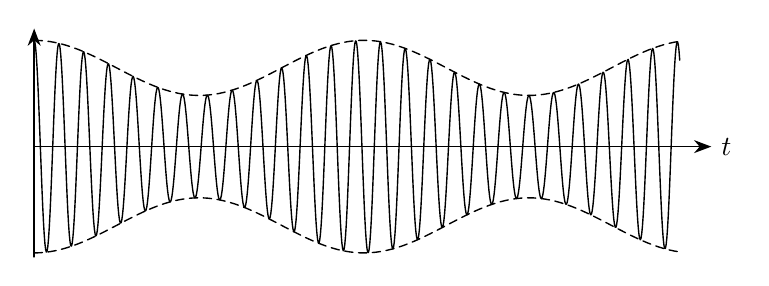
\begin{tikzpicture}[toll,x=1cm,y=1cm]
\draw[tengely] (0,-1.4) -- (0,1.5);\draw[tengely] (0,0) -- (8.6,0) node[right] {$t$};
\draw[szagg,domain=0:8.2,samples=120] plot (\x,{1+0.35*cos(\x*1.5 r)});\draw[szagg,domain=0:8.2,samples=120] plot (\x,{-1-0.35*cos(\x*1.5 r)});
\draw[line width=0.5pt,domain=0:8.2,samples=900] plot (\x,{(1+0.35*cos(\x*1.5 r))*cos(\x*20 r)});
\end{tikzpicture}
\vfill
{\small Az „5-ösöm lesz Infokommból” hallgatói gyűjtemény és a beszkennelt oktatói megoldások alapján, minden eredmény újraszámolva.\par}
\vspace{8mm}
{\small 2026. november\par}
\end{titlepage}
\chapter*{Hogyan használd ezt a könyvet}
Minden feladat ugyanúgy épül fel, hogy vizsgán is ugyanebben a rendben tudj gondolkodni.
\begin{enumerate}
\item \textbf{Feladat.} A feladat szövege, alatta a forrása (vizsga, gyűjtemény, oldal).
\item \textbf{Mit keresünk?} Minden részkérdésnél leírom, melyik mennyiséget keressük, és mit jelent.
\item \textbf{Jelölések ebben a feladatban.} Minden jel jelentése abban a környezetben, ahol épp használjuk, és ha a feladat megadja, az értéke is. Ugyanaz a betű a tárgyban több dolgot is jelenthet (a $k$ lehet Nyquist-zóna sorszáma, felharmonikus sorszáma vagy erősítési tényező), ezért ezt minden feladatnál újra rögzítem.
\item \textbf{Megoldás lépésenként.} Minden matematikai sor alatt kis kapitálissal áll a sor jellege (\textsc{tétel}, \textsc{behelyettesítés}, \textsc{számérték}, \ldots) és egy rövid megjegyzés arról, honnan jön.
\item \textbf{Eredmény}, és szükség esetén \textbf{Figyelem} doboz a tipikus hibákkal, illetve a forrásban talált tévedésekkel (\textbf{Javítás}).
\end{enumerate}

\section*{A színek jelentése}
A könyv fekete-fehér, egyedül a behelyettesítést jelzem színekkel. A feladat által megadott mennyiségek közül legfeljebb ötnek saját színe van: a jelöléstáblában, a képletben a jele, a behelyettesítésnél az értéke ugyanabban a színben jelenik meg. Így ránézésre látszik, mi hova kerül.
\begin{center}
\ca{kék}\quad \cb{narancs}\quad \cc{lila}\quad \cd{kékeszöld}\quad \ce{bíbor}
\end{center}
\behely{\bh{\ca{f_H}}{\ca{75\un{kHz}}}}
\[
f_s\ge2\,\ca{f_H}=2\cdot\ca{75}=150\un{kHz}
\]

\section*{Az ábrákról}
Ahol a feladat rajzot kér, a \textbf{Rajz: ezt kell felrajzolni} doboz pontos ábrát ad, alatta pontokba szedve, hogy kézzel mit kell feltüntetni (tengelyek, jellegzetes értékek, burkoló). Minden ábra papíron egyetlen tollal is megrajzolható.

\section*{Ellenőrzés}
Minden számértéket független szkript számolt újra (\texttt{html/check}). A források hibáit a Javítás doboz és a hibajegyzék (\texttt{03\_Hibajegyzek.md}) rögzíti.

\tableofcontents
\mainmatter
\chapter*{Jelölések jegyzéke}\addcontentsline{toc}{chapter}{Jelölések jegyzéke}\markboth{Jelölések jegyzéke}{}
A tárgyban kevés betűre sok mennyiség jut, ezért ugyanaz a jel a különböző témakörökben mást jelenthet. Az alábbi jegyzék a témakörök alapjelentéseit sorolja fel. Ha egy feladatban más a jelentés, azt a feladat „Jelölések ebben a feladatban” táblázata mondja meg, és az a mérvadó.

{\small\renewcommand{\arraystretch}{1.2}\begin{longtable}{@{}>{\raggedright\arraybackslash}p{2.4cm}>{\raggedright\arraybackslash}p{8.2cm}>{\raggedright\arraybackslash}p{3.8cm}@{}}\toprule
\textbf{Jel} & \textbf{Jelentés} & \textbf{Témakör}\\\midrule\endhead
$a$ & egy kiszolgáló kihasználtsága & VoIP, Erlang\\
$A$ & a modulátor szorzója & AM, FM\\
$A$ & a spektrum értéke 0 Hz-en & PAM, ISI\\
$A$ & felajánlott forgalom & VoIP, Erlang\\
$A_h$ & hatásos felület & Rádió\\
$A_{h,T}$ & az adóantenna hatásos felülete & Rádió\\
$a_k$ & a k-adik szimbólum amplitúdója & PAM, ISI\\
$a_\mathrm{sz}$ & szakaszcsillapítás & Rádió\\
$\alpha$ & lekerekítési tényező & QAM, PSK\\
$B$ & B paraméter a képletben & AM, FM\\
$B$ & a rendelkezésre álló sávszélesség & QAM, PSK\\
$B$ & a jel sávszélessége & Mintavétel\\
$B$ & a generátormátrix paritásrésze & Kódolás\\
$B$ & kék színjel & Hang, látás\\
$B$ & a csatorna sávszélessége & Műsorszórás\\
$B$ & egy hívás sávigénye & VoIP, Erlang\\
$\mathbf B$ & a generátormátrix paritásrésze & Kódolás\\
$B_\text{be}$ & a bemenő szűrő sávja & Mintavétel\\
$B_\text{ki}$ & a kimenő szűrő sávja & Mintavétel\\
$B_{\min}$ & a legkisebb sávszélesség & QAM, PSK\\
$B_\text{össz}$ & a jel teljes sávszélessége a pozitív frekvenciákon & Mintavétel\\
$B_v$ & a modulált jel sávszélessége & AM, FM\\
$\hat c$ & a javított (becsült) kódszó & Kódolás\\
$\hat{\mathbf c}$ & a javított (becsült) kódszó & Kódolás\\
$C$ & csúcstényező & AM, FM\\
$\mathcal C$ & a kód, a kódszavak halmaza & Kódolás\\
$C_1$ & az első kód & Kódolás\\
$C_b$ & kék színkülönbségi jel & Hang, látás\\
$c_k$ & a függőleges koordináta & QAM, PSK\\
$C_r$ & vörös színkülönbségi jel & Hang, látás\\
$d$ & átmérő & Rádió\\
$d_k$ & a vízszintes koordináta & QAM, PSK\\
$d_k$ & a k-adik szimbólum & PAM, ISI\\
$d_{\min}$ & kódtávolság, két kódszó legkisebb eltérése & Kódolás\\
$\hat{\mathbf e}$ & a becsült hibavektor & Kódolás\\
$f$ & a bemenő jel frekvenciája & Mintavétel\\
$f$ & vivőfrekvencia & Rádió\\
$f$ & frekvencia & Hang, látás\\
$F$ & vivőfrekvencia & AM, FM\\
$\mathcal F$ & a forrás (forrás ABC) & Kódolás\\
$f_0$ & a 0-s bit frekvenciája & QAM, PSK\\
$f_1$ & az 1-es bit frekvenciája & QAM, PSK\\
$f_1$ & a lapos rész vége & PAM, ISI\\
$f_2$ & ahol a spektrum eléri a nullát & PAM, ISI\\
$f_{AA}$ & a bemenő (antialiasing) szűrő határfrekvenciája & Mintavétel\\
$f_c$ & vivőfrekvencia & AM, FM\\
$f_D$ & frekvencialöket & AM, FM\\
$f_H$ & a jel legnagyobb frekvenciája & Mintavétel\\
$f_\mathrm{KF}$ & középfrekvencia & Rádió\\
$f_L$ & a jel legkisebb frekvenciája & Mintavétel\\
$f_m$ & a moduláló jel frekvenciája & AM, FM\\
$f_m$ & a moduláló (mérő)jel frekvenciája & Rádió\\
$f_\text{osc}$ & az oszcillátor frekvenciája & Rádió\\
$f_R$ & a visszaállító szűrő határfrekvenciája & Mintavétel\\
$f_s$ & mintavételi frekvencia & AM, FM\\
$f_s$ & mintavételi frekvencia (minta/s) & Kódolás\\
$f_{s,\min}$ & a legkisebb mintavételi frekvencia & Mintavétel\\
$f_t$ & tükörfrekvencia & Rádió\\
$f_v$ & vivőfrekvencia & AM, FM\\
$f_v$ & a venni kívánt adó frekvenciája & Műsorszórás\\
$G$ & antennanyereség & Rádió\\
$G$ & generátormátrix & Kódolás\\
$G$ & zöld színjel & Hang, látás\\
$\mathbf G$ & generátormátrix & Kódolás\\
$G_2$ & a második kód generátormátrixa & Kódolás\\
$G_R$ & a vevőantenna nyeresége & Rádió\\
$G_T$ & az adóantenna nyeresége & Rádió\\
$\Gamma$ & a talaj reflexiós tényezője & Rádió\\
$GI$ & a védőintervallum aránya & Műsorszórás\\
$h$ & átlagos tartási idő & VoIP, Erlang\\
$H$ & a szűrő átvitele & Mintavétel\\
$h_0$ & az elemi jel a saját mintavételi pillanatában & PAM, ISI\\
$h_1$ & az elemi jel egy jelzési idővel később & PAM, ISI\\
$H_\text{be}(f)$ & a bemenő szűrő átvitele & Mintavétel\\
$h_R$ & a vevőantenna magassága & Rádió\\
$h_T$ & az adóantenna magassága & Rádió\\
$H_V$ & a vevőszűrő átvitele & PAM, ISI\\
$H_V(f)$ & a vevőszűrő átvitele & PAM, ISI\\
$H(f)$ & az elemi jel spektruma & PAM, ISI\\
$H(f)$ & a szűrő átviteli függvénye & Mintavétel\\
$H(\mathcal F^2)$ & a szimbólumpárok entrópiája & Kódolás\\
$h(t)$ & elemi jel & PAM, ISI\\
$H^T$ & a paritásellenőrző mátrix transzponáltja & Kódolás\\
$\mathbf H^{\mathsf T}$ & a paritásellenőrző mátrix transzponáltja & Kódolás\\
$I$ & hangintenzitás & Hang, látás\\
$k$ & erősítési tényező & QAM, PSK\\
$k$ & az üzenet hossza bitben & Kódolás\\
$l$ & kódszóhossz & Kódolás\\
$L$ & átlagos kódszóhossz egy szimbólumra & Kódolás\\
$L$ & hangnyomásszint & Hang, látás\\
$\bar L$ & átlagos kódszóhossz & Kódolás\\
$L_1$ & kódszóhossz az első forrásnál & Kódolás\\
$L_1$ & a szint az első helyen & Hang, látás\\
$L_2$ & kódszóhossz a második forrásnál & Kódolás\\
$L_2$ & a szint a második helyen & Hang, látás\\
$l_a$ & az a kódszavának hossza & Kódolás\\
$l_b$ & a b kódszavának hossza & Kódolás\\
$l_c$ & a c kódszavának hossza & Kódolás\\
$l_\text{fej}$ & a fejrészek hossza & VoIP, Erlang\\
$l_i$ & az i-edik kódszó hossza & Kódolás\\
$L_N$ & hangosságszint (phon) & Hang, látás\\
$l_p$ & egy beszédszegmens hossza & VoIP, Erlang\\
$L'$ & a vevő bal kimenete & Műsorszórás\\
$L^{(2)}$ & egy szimbólumpár kódszavának hossza & Kódolás\\
$\lambda$ & hullámhossz & Rádió\\
$\lambda$ & hívásintenzitás & VoIP, Erlang\\
$m$ & modulációs mélység & AM, FM\\
$M$ & a konstelláció pontjainak száma & QAM, PSK\\
$M$ & az összegjel (L+R) & Műsorszórás\\
$\mu(t)$ & modulációs tartalom (a fázis eltérése a vivőétől) & AM, FM\\
$n$ & a kvantáló bitszáma & Mintavétel\\
$n$ & a kódszó hossza bitben & Kódolás\\
$n$ & szegmensek száma csomagonként & VoIP, Erlang\\
$N$ & a forrás szimbólumainak száma & Kódolás\\
$N$ & az OFDM-vivők száma & Műsorszórás\\
$N$ & a klaszter cellaszáma (FRF) & GSM\\
$N$ & kiszolgálók száma & VoIP, Erlang\\
$N_1$ & az első forrás szimbólumainak száma & Kódolás\\
$N_2$ & a második forrás szimbólumainak száma & Kódolás\\
$N_\text{hasznos}$ & az adatot vivő vivők száma & Műsorszórás\\
$n_{\min}$ & a legkisebb kódszóhossz & Kódolás\\
$p$ & egy bit hibavalószínűsége & Kódolás\\
$p$ & hangnyomás & Hang, látás\\
$P$ & átlagteljesítmény & AM, FM\\
$P$ & a jel teljesítménye & Mintavétel\\
$P$ & elektromos teljesítmény & Hang, látás\\
$p_0$ & a hallásküszöb hangnyomása & Hang, látás\\
$p_1$ & a keresett hangnyomás & Hang, látás\\
$p_a$ & az a szimbólum valószínűsége & Kódolás\\
$p_A$ & az A szimbólum valószínűsége & Kódolás\\
$P_a$ & az a) elrendezés átlagteljesítménye & QAM, PSK\\
$p_b$ & a b szimbólum valószínűsége & Kódolás\\
$p_B$ & a B szimbólum valószínűsége & Kódolás\\
$P_b$ & a b) elrendezés átlagteljesítménye & QAM, PSK\\
$P_b$ & blokkolási valószínűség & VoIP, Erlang\\
$p_C$ & a C szimbólum valószínűsége & Kódolás\\
$P_c$ & a c) elrendezés átlagteljesítménye & QAM, PSK\\
$P_R$ & vett teljesítmény & Rádió\\
$P_{R,\min}$ & a vevő érzékenysége (a legkisebb vehető teljesítmény) & Rádió\\
$P_T$ & adóteljesítmény & Rádió\\
$p(0)$ & a 0 szint valószínűsége & Kódolás\\
$P(0)$ & annak valószínűsége, hogy egy bit sem hibás & Kódolás\\
$P(1)$ & annak valószínűsége, hogy pontosan 1 bit hibás & Kódolás\\
$P(2)$ & annak valószínűsége, hogy pontosan 2 bit hibás & Kódolás\\
$p(\pm1)$ & a $\pm$1 szint valószínűsége & Kódolás\\
$p(\pm2)$ & a $\pm$2 szint valószínűsége & Kódolás\\
$p(\pm3)$ & a $\pm$3 szint valószínűsége & Kódolás\\
$\Phi_D$ & fázislöket & AM, FM\\
$r$ & az adó és a vevő távolsága & Rádió\\
$r$ & szimbólumsebesség (szimbólum/s) & Kódolás\\
$R$ & terhelő ellenállás & AM, FM\\
$R$ & az ellenállás & Mintavétel\\
$R$ & a parabola sugara & Rádió\\
$R$ & vörös színjel & Hang, látás\\
$r_0$ & a zónahatár távolsága & Rádió\\
$r_1$ & az első távolság & Hang, látás\\
$r_2$ & a második távolság & Hang, látás\\
$r_{\max}$ & a legnagyobb távolság & Rádió\\
$R_s$ & szimbólumsebesség & QAM, PSK\\
$R'$ & a vevő jobb kimenete & Műsorszórás\\
$RC$ & a burkolódemodulátor időállandója & AM, FM\\
$s$ & szindróma & Kódolás\\
$\hat s$ & a modulált jel csúcsértéke & AM, FM\\
$S$ & a különbségi (L$-$R) jel & Műsorszórás\\
$s_0$ & a teljesítménysűrűség & Mintavétel\\
$s_\mathrm{FM}(t)$ & az FM-jel & AM, FM\\
$s_m(t)$ & a moduláló jel & AM, FM\\
$s(t)$ & a modulált jel & AM, FM\\
$\text{SNR}$ & jel-zaj viszony & AM, FM\\
$\Delta\text{SNR}$ & a jel-zaj viszony változása & AM, FM\\
$T$ & jelzési (bit-) idő & QAM, PSK\\
$T$ & jelzési idő & PAM, ISI\\
$T$ & mintavételi idő & Mintavétel\\
$t_0$ & a mintavétel helye a jelzési időn belül & PAM, ISI\\
$T_0$ & a moduláló jel félperiódusa & AM, FM\\
$T_0$ & a mintavétel helye a jelzési időn belül & PAM, ISI\\
$T_0$ & hasznos szimbólumidő & Műsorszórás\\
$T_1$ & első mintavételi idő & Mintavétel\\
$T_2$ & második mintavételi idő & Mintavétel\\
$T_m$ & a moduláló jel periódusideje & AM, FM\\
$\hat u$ & a becsült üzenet & Kódolás\\
$\hat{\mathbf u}$ & a becsült üzenet & Kódolás\\
$U$ & a modulált jel amplitúdója & AM, FM\\
$U$ & a jel amplitúdója & QAM, PSK\\
$U$ & a bemenő jel amplitúdója & Mintavétel\\
$U_0$ & egyenszint (a burkoló középértéke) & AM, FM\\
$U_{6{,}2}$ & a kimenő 6,2 kHz-es összetevő amplitúdója & Mintavétel\\
$U_m$ & a burkoló kilengése & AM, FM\\
$v$ & bitsebesség & QAM, PSK\\
$v$ & a vett szó & Kódolás\\
$\mathbf v$ & a vett szó & Kódolás\\
$v_\text{cs}$ & csomagsebesség & VoIP, Erlang\\
$v_\text{forrás}$ & a kodek bitsebessége & VoIP, Erlang\\
$v_\text{nettó}$ & nettó bitsebesség & Műsorszórás\\
$V(\lambda)$ & láthatósági függvény & Hang, látás\\
$\varphi$ & fázishiba & QAM, PSK\\
$\varphi_{\max}$ & a megengedett fázishiba & QAM, PSK\\
$\hat x$ & a jel csúcsértéke & AM, FM\\
$x(t)$ & a moduláló jel & AM, FM\\
$x(t)$ & a PAM-jel & PAM, ISI\\
$Y$ & világossági jel & Hang, látás\\
\bottomrule\end{longtable}}
% Generálva: html/build_tex.js (o01.js). Kézzel ne szerkeszd, a forrás a html/data mappa.
\setcounter{chapter}{0}
\chapter{\texorpdfstring{Analóg moduláció (AM, FM, szögmoduláció)}{Analóg moduláció (AM, FM, szögmoduláció)}}\label{f1}
A gyűjtemény első fejezete: csúcstényező, FM-jel képletből és oszcilloszkópról, AM-jel rajza és spektruma. Minden példa elején ott van, mit jelentenek a jelek, és minden szám mellett, honnan jön.

\section{Alapok, egyszerűen}
\subsection{\texorpdfstring{A1. Jelölések ebben a fejezetben}{A1. Jelölések ebben a fejezetben}}\label{b1-jel}
\par\noindent{\small\renewcommand{\arraystretch}{1.25}\begin{tabularx}{\linewidth}{@{}>{\raggedright\arraybackslash}X>{\raggedright\arraybackslash}X>{\raggedright\arraybackslash}X@{}}\toprule
\textbf{Jel} & \textbf{Jelentés} & \textbf{Egység}\\\midrule
undefined & vivőfrekvencia: a modulálatlan vivő frekvenciája & Hz\\
undefined & a moduláló (az átvinni kívánt) jel frekvenciája & Hz\\
undefined & a vivő amplitúdója (AM-nél a burkoló középértéke) & V\\
undefined & a burkoló kilengése a középérték körül (AM) & V\\
undefined & modulációs mélység, undefined & 1 vagy \%\\
undefined & modulációs tartalom szögmodulációnál: ennyivel tér el a jel fázisa a vivőétől & rad\\
undefined & fázislöket: undefined legnagyobb abszolút értéke & rad\\
undefined & frekvencialöket: a pillanatnyi frekvencia legnagyobb eltérése undefined-től & Hz\\
undefined & a modulált jel sávszélessége & Hz\\
undefined & csúcstényező: csúcsérték osztva az effektív értékkel & 1\\
undefined & átlagteljesítmény, ha nincs más megadva, 1 $\Omega$-on: undefined & W\\
\bottomrule\end{tabularx}}\par

\subsection{\texorpdfstring{A2. AM-DSB: képlet, spektrum, teljesítmény}{A2. AM-DSB: képlet, spektrum, teljesítmény}}\label{b1-am}
\begin{center}\adjustbox{max width=\linewidth}{$\displaystyle s(t)=\left[U_v+U_m\cos(2\pi f_mt)\right]\cos(2\pi f_vt)$}\end{center}

A szögletes zárójel a \textbf{burkoló}: $U_v-U_m$ és $U_v+U_m$ között ingadozik. A jel csúcsértéke ezért $U_v+U_m=U_v(1+m)$.

A spektrum a $\cos a\cos b=\tfrac12\left[\cos(a-b)+\cos(a+b)\right]$ azonosságból jön:

\begin{center}\adjustbox{max width=\linewidth}{$\displaystyle s(t)=U_v\cos2\pi f_vt+\frac{U_m}{2}\cos2\pi(f_v-f_m)t+\frac{U_m}{2}\cos2\pi(f_v+f_m)t$}\end{center}

Három vonal: a vivő $U_v$ amplitúdóval, és a két oldalsáv egyenként $U_m/2$-vel. Egy $A$ amplitúdójú szinusz teljesítménye 1 $\Omega$-on $A^2/2$ (mert $\sin^2$ átlaga $1/2$), a különböző frekvenciájú vonalak teljesítménye összeadódik.

Burkolódemodulátor (dióda, utána párhuzamos RC) akkor használható, ha $m\le1$, azaz a burkoló nem megy nulla alá. Az RC-taggal szemben két feltétel van: a kondenzátor tartsa a feszültséget két vivőcsúcs között ($RC\gg1/f_v$), de kövesse a burkoló változását ($RC\ll1/f_m$).

\subsection{\texorpdfstring{A3. Szögmoduláció: PM és FM}{A3. Szögmoduláció: PM és FM}}\label{b1-fm}
\begin{center}\adjustbox{max width=\linewidth}{$\displaystyle s(t)=U\cos\left(2\pi f_vt+\mu(t)\right)$}\end{center}

Az amplitúdó állandó, a fázis változik. \textbf{PM}-nél maga $\mu(t)$ arányos a moduláló jellel, \textbf{FM}-nél a deriváltja, $\mu'(t)$. A pillanatnyi frekvencia $f(t)=f_v+\tfrac1{2\pi}\mu'(t)$, ezért

\begin{center}\adjustbox{max width=\linewidth}{$\displaystyle \Phi_D=\max|\mu(t)|\qquad f_D=\frac1{2\pi}\max|\mu'(t)|$}\end{center}

Szinuszos modulációnál $\mu(t)=\Phi_D\sin(2\pi f_mt)$, a deriváltja $2\pi f_m\Phi_D\cos(2\pi f_mt)$, így $f_D=\Phi_Df_m$. A sávszélességet a \textbf{Carson-szabály} becsüli (ebben van a teljesítmény kb. 98\%-a):

\begin{center}\adjustbox{max width=\linewidth}{$\displaystyle B_v\approx2(f_D+f_m)$}\end{center}

A szögmodulált jel teljesítménye $U^2/2$, a modulációtól független, a csúcstényezője $\sqrt2$, mint bármely állandó amplitúdójú szinuszé.

% ------------------------------------------------------------------
\section{\texorpdfstring{1.1. feladat: $3\sin+4\cos$ csúcstényezője, maximuma, teljesítménye}{1.1. feladat: 3sin+4cos csúcstényezője, maximuma, teljesítménye}}\label{o1_01}
\setcounter{lepes}{0}
\begin{feladat}{1.1. feladat}
Határozza meg az $x(t)=3\sin(2\pi Ft)+4\cos(2\pi Ft)$ jel csúcstényezőjét, maximális értékét és teljesítményét!

{\footnotesize\sffamily Forrás: 5-ösöm 2. oldal $\cdot$ 5o\_02\_1. Címkék: beugró, javítás}
\end{feladat}
\begin{keresunk}
\begin{itemize}
\item $C$: csúcstényező, $\hat x/x_\text{eff}$
\item $\hat x$: a jel legnagyobb értéke
\item $P$: átlagteljesítmény (1 $\Omega$-on, $P=x_\text{eff}^2$)
\end{itemize}
\end{keresunk}
\begin{jeloles}
\begin{jeltabla}
$F$ & vivőfrekvencia & \\
$C$ & csúcstényező & \emph{keresett}\\
$\hat x$ & a jel csúcsértéke & \emph{keresett}\\
$P$ & átlagteljesítmény & \emph{keresett}\\
$A$ & az összevont szinusz amplitúdója & \\
$\omega$ & körfrekvencia, $\omega=2\pi F$ & \\
$\varphi$ & az összevont szinusz kezdőfázisa & \\
\end{jeltabla}
\par\smallskip\textbf{Adott még:}
\begin{itemize}
\item $x(t)$: két azonos, $F$ frekvenciájú tag összege, a szinuszos tag amplitúdója 3, a koszinuszosé 4 (a feladatból)
\item $F$: a két tag közös frekvenciája. Az értéke nem kell, az eredmény nem függ tőle
\end{itemize}
\end{jeloles}
\begin{elmelet}[Miért így? Egyszerűen]
\textbf{Miért lehet egyetlen szinusszá összevonni?}\par Két azonos frekvenciájú szinuszos jel összege mindig ugyanolyan frekvenciájú szinusz, csak más amplitúdóval és fázissal. Ebből a csúcsérték közvetlenül leolvasható.
\end{elmelet}

\lepes{Összevonás egyetlen szinusszá}
Keressük $A\sin(\omega t+\varphi)$ alakban, $\omega=2\pi F$. Az addíciós tétellel kifejtjük, és a $\sin\omega t$, illetve $\cos\omega t$ együtthatóit egyeztetjük a feladatbeli 3-mal és 4-gyel.

\begin{center}\adjustbox{max width=\linewidth}{$\displaystyle A\sin(\omega t+\varphi)=A\cos\varphi\,\sin\omega t+A\sin\varphi\,\cos\omega t$}\end{center}
\jegyzet{tétel}{addíciós tétel}

\begin{center}\adjustbox{max width=\linewidth}{$\displaystyle A\cos\varphi=3\qquad A\sin\varphi=4$}\end{center}
\jegyzet{átalakítás}{a feladat együtthatóival egyeztetve}

\begin{center}\adjustbox{max width=\linewidth}{$\displaystyle A^2(\cos^2\varphi+\sin^2\varphi)=3^2+4^2\ \Rightarrow\ A=\sqrt{25}=5$}\end{center}
\jegyzet{átalakítás}{a két egyenletet négyzetre emelve és összeadva}

\begin{center}\adjustbox{max width=\linewidth}{$\displaystyle \mathrm{tg}\,\varphi=\tfrac43\ \Rightarrow\ \varphi=53{,}1^{\circ}$}\end{center}
\jegyzet{számérték}{a fázis az eredményhez nem kell}

\lepes{b) A maximális érték}
$5\sin(\omega t+\varphi)$ legnagyobb értéke ott van, ahol a szinusz 1.

\begin{center}\adjustbox{max width=\linewidth}{$\displaystyle \hat x=5\cdot1=5$}\end{center}
\jegyzet{számérték}{}

\lepes{c) A teljesítmény}
Egy $A$ amplitúdójú szinusz négyzetének átlaga $A^2/2$, mert $\sin^2$ átlaga egy perióduson $1/2$.

\begin{center}\adjustbox{max width=\linewidth}{$\displaystyle P=\overline{x^2}=\frac{A^2}{2}=\frac{5^2}{2}=12{,}5\ \text{W}$}\end{center}
\jegyzet{definíció}{1 $\Omega$-on, $A=5$ az első lépésből}

\begin{center}\adjustbox{max width=\linewidth}{$\displaystyle \frac{3^2}{2}+\frac{4^2}{2}=4{,}5+8=12{,}5$}\end{center}
\jegyzet{ellenőrzés}{a $\sin$ és a $\cos$ szorzatának átlaga 0, ezért a két tag teljesítménye összeadódik}

\lepes{a) A csúcstényező}
Az effektív érték a teljesítmény gyöke, a csúcstényező a csúcsérték és az effektív érték hányadosa.

\begin{center}\adjustbox{max width=\linewidth}{$\displaystyle x_\text{eff}=\sqrt{P}=\sqrt{12{,}5}=3{,}54$}\end{center}
\jegyzet{definíció}{$P$ a c) részből}

\begin{center}\adjustbox{max width=\linewidth}{$\displaystyle C=\frac{\hat x}{x_\text{eff}}=\frac{5}{3{,}54}=1{,}414=\sqrt2$}\end{center}
\jegyzet{számérték}{$\hat x$ a b) részből}
\begin{eredmeny}

\begin{center}\adjustbox{max width=\linewidth}{$\displaystyle \text{a) }C=\sqrt2\qquad\text{b) }\hat x=5\qquad\text{c) }P=12{,}5\ \text{W (1 }\Omega\text{-on)}$}\end{center}
\end{eredmeny}
\begin{tipp}[Ellenőrzés]
\begin{itemize}
\item Bármely szinuszos jel csúcstényezője $\sqrt2$, az amplitúdótól függetlenül. Mivel az összeg is szinusz, $C=\sqrt2$ számolás nélkül is várható volt.
\end{itemize}
\end{tipp}
\begin{figyelem}[Tipikus hibák]
\begin{itemize}
\item A maximumot ott keresni, ahol $\sin=\cos$ (45\textdegree{}-nál): ott $3/\sqrt2+4/\sqrt2=4{,}95$, ez kisebb 5-nél. A maximum $\varphi=53{,}1^{\circ}$-nál van.
\end{itemize}
\end{figyelem}


% ------------------------------------------------------------------
\section{\texorpdfstring{1.2. feladat: FM-jel képletből: 500 kHz, 5 rad}{1.2. feladat: FM-jel képletből: 500 kHz, 5 rad}}\label{o1_02}
\setcounter{lepes}{0}
\begin{feladat}{1.2. feladat}
$s_m(t)=3\cos(3\pi t+2)$ bemenetre $s_\mathrm{FM}(t)=5\cos(1000\pi t+9+5\sin(3\pi t+2))$, $t$ ms-ban. a) Vivőfrekvencia és fázislöket? b) Demodulátor blokkvázlata?

{\footnotesize\sffamily Forrás: 5-ösöm 2. oldal $\cdot$ 5o\_02\_2. Címkék: vizsga}
\end{feladat}
\begin{keresunk}
\begin{itemize}
\item a) $f_v$: vivőfrekvencia, és $\Phi_D$: fázislöket (a fázis legnagyobb eltérése a vivőétől, rad)
\item b) a demodulátor felépítése
\end{itemize}
\end{keresunk}
\begin{jeloles}
\begin{jeltabla}
$f_v$ & vivőfrekvencia & \emph{keresett}\\
$\Phi_D$ & fázislöket & \emph{keresett}\\
$U$ & a modulált jel amplitúdója & \\
$\varphi_0$ & kezdőfázis & \\
$\mu$ & a modulációs tartalom (a fázis eltérése a vivőétől), $\mu$(t) & \\
$f_m$ & a moduláló jel frekvenciája & \\
$f_D$ & frekvencialöket & \\
$B_v$ & a modulált jel sávszélessége & \\
$f$ & a pillanatnyi frekvencia & \\
\end{jeltabla}
\par\smallskip\textbf{Adott még:}
\begin{itemize}
\item $t$ ms-ban: a $t$ együtthatói rad/ms-ban értendők
\end{itemize}
\end{jeloles}

\lepes{A képlet összevetése az általános alakkal}
Az általános alak $U\cos(2\pi f_vt+\varphi_0+\mu(t))$. A koszinusz argumentumában három rész van: a $t$-vel arányos tag a vivőé, az állandó (9 rad) csak egy kezdőfázis, a $t$-től függő maradék a modulációs tartalom.

\begin{center}\adjustbox{max width=\linewidth}{$\displaystyle U=5\ \text{V}\qquad\varphi_0=9\ \text{rad}\qquad\mu(t)=5\sin(3\pi t+2)$}\end{center}
\jegyzet{definíció}{leolvasva $s_\mathrm{FM}$-ből}

\lepes{a) A vivőfrekvencia}
A vivő tagja $2\pi f_vt$. Ezt egyeztetjük $1000\pi t$-vel. Mivel $t$ ms-ban van, a kapott frekvencia kHz-ben értendő.

\begin{center}\adjustbox{max width=\linewidth}{$\displaystyle 2\pi f_vt=1000\pi t\ \Rightarrow\ f_v=\frac{1000\pi}{2\pi}=500\ \tfrac1{\text{ms}}=500\ \text{kHz}$}\end{center}
\jegyzet{átalakítás}{$1/\text{ms}=1$ kHz}

\lepes{a) A fázislöket}
A fázislöket $\mu(t)$ legnagyobb abszolút értéke. A szinusz legnagyobb értéke 1.

\begin{center}\adjustbox{max width=\linewidth}{$\displaystyle \Phi_D=\max|5\sin(3\pi t+2)|=5\ \text{rad}$}\end{center}
\jegyzet{definíció}{}

\lepes{Kiegészítés: FM-e, és mekkora a frekvencialöket?}
A moduláló jel frekvenciája a $3\pi t$ tagból jön. A fázis deriváltja koszinusz, ugyanazzal az argumentummal, mint $s_m(t)$, tehát a derivált arányos a moduláló jellel: ez FM.

\begin{center}\adjustbox{max width=\linewidth}{$\displaystyle 2\pi f_m=3\pi\ \Rightarrow\ f_m=1{,}5\ \text{kHz}$}\end{center}
\jegyzet{átalakítás}{a $3\pi t$ tagból, szintén kHz}

\begin{center}\adjustbox{max width=\linewidth}{$\displaystyle \mu'(t)=5\cdot3\pi\cos(3\pi t+2)=5\pi\,s_m(t)$}\end{center}
\jegyzet{deriválás}{arányos $s_m(t)$-vel: FM}

\begin{center}\adjustbox{max width=\linewidth}{$\displaystyle f_D=\frac{\max|\mu'|}{2\pi}=\frac{15\pi}{2\pi}=7{,}5\ \text{kHz}=\Phi_Df_m$}\end{center}
\jegyzet{számérték}{}

\begin{center}\adjustbox{max width=\linewidth}{$\displaystyle B_v\approx2(f_D+f_m)=2(7{,}5+1{,}5)=18\ \text{kHz}$}\end{center}
\jegyzet{tétel}{Carson-szabály}

\lepes{b) A demodulátor}
Számláló típusú FM-demodulátor: \textbf{nullátmenet-detektor} (minden nullátmenetnél jelez) $\to$ \textbf{impulzusgenerátor} (minden jelzésre egy azonos alakú impulzust ad) $\to$ \textbf{aluláteresztő szűrő} (átlagol). Minél nagyobb a pillanatnyi frekvencia, annál sűrűbbek a nullátmenetek, annál nagyobb az átlag: a kimenet arányos $f(t)-f_v$-vel, azaz a moduláló jellel.

\begin{rajz}
\textbf{Számláló típusú FM-demodulátor}\par
\begin{center}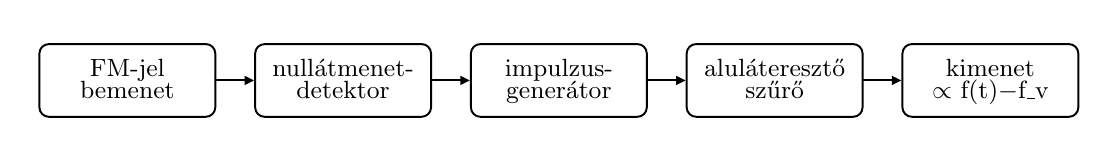
\begin{tikzpicture}[x=0.01490cm,y=-0.01490cm,line cap=round,line join=round]
\useasboundingbox (0,0) rectangle (906,90);
\path[draw=black,line width=0.7pt,rounded corners=0.12cm] (10,14) rectangle (160,76);
\node[anchor=base,inner sep=0pt,font=\small] at (85,41.5) {FM-jel};
\node[anchor=base,inner sep=0pt,font=\small] at (85,60.5) {bemenet};
\path[draw=black,line width=0.7pt] (160,45) -- (186,45);
\path[fill=black,draw=none] (193,45) -- (185,41) -- (185,49) -- cycle;
\path[draw=black,line width=0.7pt,rounded corners=0.12cm] (194,14) rectangle (344,76);
\node[anchor=base,inner sep=0pt,font=\small] at (269,41.5) {nullátmenet-};
\node[anchor=base,inner sep=0pt,font=\small] at (269,60.5) {detektor};
\path[draw=black,line width=0.7pt] (344,45) -- (370,45);
\path[fill=black,draw=none] (377,45) -- (369,41) -- (369,49) -- cycle;
\path[draw=black,line width=0.7pt,rounded corners=0.12cm] (378,14) rectangle (528,76);
\node[anchor=base,inner sep=0pt,font=\small] at (453,41.5) {impulzus-};
\node[anchor=base,inner sep=0pt,font=\small] at (453,60.5) {generátor};
\path[draw=black,line width=0.7pt] (528,45) -- (554,45);
\path[fill=black,draw=none] (561,45) -- (553,41) -- (553,49) -- cycle;
\path[draw=black,line width=0.7pt,rounded corners=0.12cm] (562,14) rectangle (712,76);
\node[anchor=base,inner sep=0pt,font=\small] at (637,41.5) {aluláteresztő};
\node[anchor=base,inner sep=0pt,font=\small] at (637,60.5) {szűrő};
\path[draw=black,line width=0.7pt] (712,45) -- (738,45);
\path[fill=black,draw=none] (745,45) -- (737,41) -- (737,49) -- cycle;
\path[draw=black,line width=0.7pt,rounded corners=0.12cm] (746,14) rectangle (896,76);
\node[anchor=base,inner sep=0pt,font=\small] at (821,41.5) {kimenet};
\node[anchor=base,inner sep=0pt,font=\small] at (821,60.5) {$\propto$ f(t)$-$f\_v};
\end{tikzpicture}\end{center}
\begin{itemize}
\item Négy doboz, balról jobbra. A nullátmenet-detektor minden nullátmenetnél jelez, az impulzusgenerátor minden jelzésre egy azonos alakú impulzust ad, az aluláteresztő átlagol.
\item A kimenet annál nagyobb, minél sűrűbbek a nullátmenetek, vagyis a pillanatnyi frekvenciával arányos.
\end{itemize}
\end{rajz}
\begin{eredmeny}

\begin{center}\adjustbox{max width=\linewidth}{$\displaystyle \text{a) }f_v=500\ \text{kHz},\ \Phi_D=5\ \text{rad}\quad(f_D=7{,}5\ \text{kHz},\ B_v\approx18\ \text{kHz})\qquad\text{b) számláló típusú demodulátor}$}\end{center}
\end{eredmeny}
\begin{figyelem}[Tipikus hibák]
\begin{itemize}
\item A 9 rad-os állandót löketnek venni: az csak kezdőfázis, nem változik az idővel.
\item Elfelejteni, hogy $t$ ms-ban van: $1000\pi/(2\pi)=500$ ekkor kHz, nem Hz.
\end{itemize}
\end{figyelem}


% ------------------------------------------------------------------
\section{\texorpdfstring{1.3. feladat: Milyen moduláció? 250 kHz, 18 kHz-es sáv}{1.3. feladat: Milyen moduláció? 250 kHz, 18 kHz-es sáv}}\label{o1_03}
\setcounter{lepes}{0}
\begin{feladat}{1.3. feladat}
$s_m(t)=3\cos(3\pi t+2)$ V bemenetre $s(t)=4\cos(500\pi t+21+5\sin(3\pi t+2))$ V ($t$ ms-ban). a) Moduláció fajtája? b) Amplitúdók? c) Fázis- és frekvencialöket? d) Vivő és sávszélesség?

{\footnotesize\sffamily Forrás: 5-ösöm 3. oldal $\cdot$ 5o\_03\_1 (gépelt megoldás). Címkék: vizsga}
\end{feladat}
\begin{keresunk}
\begin{itemize}
\item a) FM vagy PM
\item b) a moduláló és a modulált jel amplitúdója
\item c) $\Phi_D$ (fázislöket, rad) és $f_D$ (frekvencialöket, kHz)
\item d) $f_v$ (vivőfrekvencia) és $B_v$ (sávszélesség)
\end{itemize}
\end{keresunk}
\begin{jeloles}
\begin{jeltabla}
$\Phi_D$ & fázislöket & \emph{keresett}\\
$f_D$ & frekvencialöket & \emph{keresett}\\
$f_v$ & vivőfrekvencia & \emph{keresett}\\
$B_v$ & a modulált jel sávszélessége & \emph{keresett}\\
$\mu$ & a modulációs tartalom (a fázis eltérése a vivőétől), $\mu$(t) & \\
$\hat s_m$ & a moduláló jel csúcsértéke & \\
$\hat s$ & a modulált jel csúcsértéke & \\
$f_m$ & a moduláló jel frekvenciája & \\
\end{jeltabla}
\end{jeloles}
\begin{elmelet}[Miért így? Egyszerűen]
\textbf{Miért FM és nem PM?}\par A moduláló jel koszinusz, a modulációs tartalom szinusz ugyanazzal az argumentummal: a tartalom \textbf{deriváltja} (koszinusz) arányos a moduláló jellel. PM-nél maga a tartalom lenne koszinusz.
\end{elmelet}

\lepes{a) A moduláció fajtája}
A koszinusz argumentumának $t$-től függő, nem lineáris része a modulációs tartalom.

\begin{center}\adjustbox{max width=\linewidth}{$\displaystyle \mu(t)=5\sin(3\pi t+2)$}\end{center}
\jegyzet{definíció}{leolvasva $s(t)$-ből, a 21 rad csak kezdőfázis}

\begin{center}\adjustbox{max width=\linewidth}{$\displaystyle \mu'(t)=15\pi\cos(3\pi t+2)=5\pi\cdot s_m(t)$}\end{center}
\jegyzet{deriválás}{arányos $s_m$-mel: \textbf{FM}}

\lepes{b) Amplitúdók}
A koszinuszok előtti szorzók.

\begin{center}\adjustbox{max width=\linewidth}{$\displaystyle \hat s_m=3\ \text{V}\qquad\hat s=4\ \text{V}$}\end{center}
\jegyzet{számérték}{a feladat képleteiből}

\lepes{c) Löketek}
A moduláló frekvencia a $3\pi t$ tagból: $2\pi f_m=3\pi$, $t$ ms-ban, tehát kHz.

\begin{center}\adjustbox{max width=\linewidth}{$\displaystyle f_m=\frac{3\pi}{2\pi}=1{,}5\ \text{kHz}$}\end{center}
\jegyzet{átalakítás}{}

\begin{center}\adjustbox{max width=\linewidth}{$\displaystyle \Phi_D=\max|\mu|=5\ \text{rad}$}\end{center}
\jegyzet{definíció}{a szinusz legnagyobb értéke 1}

\begin{center}\adjustbox{max width=\linewidth}{$\displaystyle f_D=\frac{\max|\mu'|}{2\pi}=\frac{5\cdot3\pi}{2\pi}=7{,}5\ \text{kHz}$}\end{center}
\jegyzet{definíció}{ugyanez $\Phi_Df_m=5\cdot1{,}5$}

\lepes{d) Vivő és sávszélesség}
A vivő tagja $500\pi t$. A sávszélességet a Carson-szabály adja, mert szinuszos modulációjú FM-jelről van szó.

\begin{center}\adjustbox{max width=\linewidth}{$\displaystyle 2\pi f_v=500\pi\ \Rightarrow\ f_v=250\ \text{kHz}$}\end{center}
\jegyzet{átalakítás}{}

\begin{center}\adjustbox{max width=\linewidth}{$\displaystyle B_v\approx2(f_D+f_m)=2(7{,}5+1{,}5)=18\ \text{kHz}$}\end{center}
\jegyzet{tétel}{$f_D$ és $f_m$ a c) részből}
\begin{eredmeny}

\begin{center}\adjustbox{max width=\linewidth}{$\displaystyle \text{a) FM}\quad\text{b) 3 V és 4 V}\quad\text{c) }\Phi_D=5\ \text{rad},\ f_D=7{,}5\ \text{kHz}\quad\text{d) }f_v=250\ \text{kHz},\ B_v\approx18\ \text{kHz}$}\end{center}
\end{eredmeny}


% ------------------------------------------------------------------
\section{\texorpdfstring{1.4. feladat: AM-DSB: 60 kHz, 20\%, 1,8 V csúcs}{1.4. feladat: AM-DSB: 60 kHz, 20, 1,8 V csúcs}}\label{o1_04}
\setcounter{lepes}{0}
\begin{feladat}{1.4. feladat}
60 kHz-es vivő, 10 kHz-es szinusz, $m=20\%$, csúcsérték 1,8 V. a) Rajz (200 \textmu{}s). b) Időfüggvény, komponensek, a moduláló jel amplitúdója. c) Demodulátor és specifikációja.

{\footnotesize\sffamily Forrás: 5-ösöm 3. oldal $\cdot$ 5o\_03\_2. Címkék: vizsga}
\end{feladat}
\begin{keresunk}
\begin{itemize}
\item a) a jel rajza 200 \textmu{}s hosszan
\item b) $s(t)$ (a modulált jel), a spektrumvonalak, $U_m$ (a burkoló kilengése)
\item c) a demodulátor és az $RC$ (a burkolódemodulátor időállandója) időállandó
\end{itemize}
\end{keresunk}
\begin{jeloles}
\begin{jeltabla}
$\ca{f_v}$ & vivőfrekvencia & $60$\,kHz\\
$\cb{f_m}$ & a moduláló jel frekvenciája & $10$\,kHz\\
$\cc{m}$ & modulációs mélység & $0{,}2$\\
$\hat s$ & a modulált jel csúcsértéke & \\
$U_m$ & a burkoló kilengése & \emph{keresett}\\
$RC$ & a burkolódemodulátor időállandója & \emph{keresett}\\
$U_v$ & a vivő amplitúdója & \\
$a$ & tetszőleges szög (az azonosság első változója) & \\
$b$ & tetszőleges szög (az azonosság második változója) & \\
$T_m$ & a moduláló jel periódusideje & \\
$T_v$ & a vivő periódusideje & \\
\end{jeltabla}
\end{jeloles}

\lepes{A modell}
AM-DSB szinuszos modulációval (A2). A burkoló legnagyobb értéke $U_v+U_m=U_v(1+{\cc{m}})$, és a jel csúcsértéke ezzel egyezik, mert a vivő ott is eléri az 1-et.

\begin{center}\adjustbox{max width=\linewidth}{$\displaystyle s(t)=\left[U_v+U_m\cos(2\pi f_mt)\right]\cos(2\pi f_vt),\qquad U_m=mU_v$}\end{center}
\jegyzet{definíció}{}

\lepes{b) Amplitúdók}
A csúcsértékből és ${\cc{m}}$-ből kifejezzük $U_v$-t, abból $U_m$-et.
\behely{\bh{\cc{m}}{\cc{0{,}2}}}

\begin{center}\adjustbox{max width=\linewidth}{$\displaystyle U_v(1+{\cc{0{,}2}})=1{,}8\ \Rightarrow\ U_v=\frac{1{,}8}{1{,}2}=1{,}5\ \text{V}$}\end{center}
\jegyzet{behelyettesítés}{$\hat s=1{,}8$ V és $m=0{,}2$ a feladatból}

\begin{center}\adjustbox{max width=\linewidth}{$\displaystyle U_m=mU_v={\cc{0{,}2}}\cdot1{,}5=0{,}3\ \text{V}$}\end{center}
\jegyzet{számérték}{a moduláló jel amplitúdója a burkolón}

\lepes{b) Időfüggvény}
A frekvenciák kHz-ben vannak, ezért az időt ms-ban írjuk, így a szorzat egység nélküli.
\behely{\bh{\ca{f_v}}{\ca{60\un{kHz}}}}

\begin{center}\adjustbox{max width=\linewidth}{$\displaystyle s(t)=\left[1{,}5+0{,}3\cos(2\pi\cdot10\,t)\right]\cos(2\pi\cdot{\ca{60}}\,t)\ \text{V},\quad[t]=\text{ms}$}\end{center}
\jegyzet{behelyettesítés}{}

\lepes{b) Spektrum}
A $\cos a\cos b=\tfrac12[\cos(a-b)+\cos(a+b)]$ azonosság a $0{,}3\cos\cdot\cos$ szorzatból két oldalsávot csinál, mindegyik $U_m/2$ amplitúdóval.

\begin{center}\adjustbox{max width=\linewidth}{$\displaystyle 0{,}3\cos(2\pi\cdot10t)\cos(2\pi\cdot{\ca{60}}t)=0{,}15\cos(2\pi\cdot50t)+0{,}15\cos(2\pi\cdot70t)$}\end{center}
\jegyzet{tétel}{}

\begin{center}\adjustbox{max width=\linewidth}{$\displaystyle {\ca{60}}\ \text{kHz: }1{,}5\ \text{V}\qquad50\ \text{és}\ 70\ \text{kHz: }0{,}15\ \text{V}$}\end{center}
\jegyzet{számérték}{$f_v$ és $f_v\pm f_m$}

\lepes{a) A rajz}
200 \textmu{}s-ba ennyi periódus fér. A burkoló $U_v-U_m=1{,}2$ V és $U_v+U_m=1{,}8$ V között ingadozik, a jel a burkoló és a tükörképe között rezeg.

\begin{center}\adjustbox{max width=\linewidth}{$\displaystyle T_m=\frac1{10\ \text{kHz}}=100\ \mu\text{s}\ \Rightarrow\ 2\ \text{moduláló periódus}$}\end{center}
\jegyzet{számérték}{}

\begin{center}\adjustbox{max width=\linewidth}{$\displaystyle T_v=\frac1{60\ \text{kHz}}=16{,}7\ \mu\text{s}\ \Rightarrow\ \frac{200}{16{,}7}=12\ \text{vivőperiódus}$}\end{center}
\jegyzet{számérték}{}

\lepes{c) Demodulátor}
Mivel ${\cc{m}}={\cc{0{,}2}}\le1$, a burkoló sosem megy nulla alá, ezért burkolódemodulátor (dióda + párhuzamos RC) használható. Az RC két vivőcsúcs között tartsa a feszültséget, de a burkolót kövesse.

\begin{center}\adjustbox{max width=\linewidth}{$\displaystyle T_v=16{,}7\ \mu\text{s}\ \ll\ RC\ \ll\ T_m=100\ \mu\text{s}$}\end{center}
\jegyzet{közelítés}{$T_v$ és $T_m$ az előző lépésből}

\begin{center}\adjustbox{max width=\linewidth}{$\displaystyle RC\approx\sqrt{16{,}7\cdot100}\ \mu\text{s}\approx40\ \mu\text{s}$}\end{center}
\jegyzet{számérték}{a két határ mértani közepe jó választás}

\begin{rajz}
\textbf{Időfüggvény, 200 \textmu{}s}\par
\begin{center}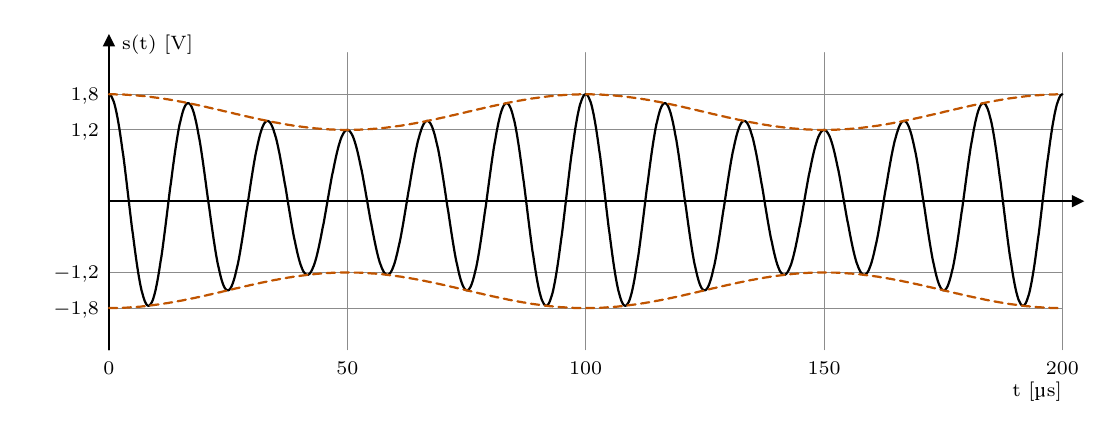
\begin{tikzpicture}[x=0.01985cm,y=-0.01985cm,line cap=round,line join=round]
\useasboundingbox (0,0) rectangle (680,240);
\path[draw=black!45,line width=0.35pt] (52,206) -- (52,16);
\path[draw=black!45,line width=0.35pt] (204.5,206) -- (204.5,16);
\path[draw=black!45,line width=0.35pt] (357,206) -- (357,16);
\path[draw=black!45,line width=0.35pt] (509.5,206) -- (509.5,16);
\path[draw=black!45,line width=0.35pt] (662,206) -- (662,16);
\path[draw=black!45,line width=0.35pt] (52,42.6) -- (662,42.6);
\path[draw=black!45,line width=0.35pt] (52,65.4) -- (662,65.4);
\path[draw=black!45,line width=0.35pt] (52,156.6) -- (662,156.6);
\path[draw=black!45,line width=0.35pt] (52,179.4) -- (662,179.4);
\path[draw=black,line width=0.7pt] (52,111) -- (670,111);
\path[fill=black,draw=none] (676,111) -- (668,107) -- (668,115) -- cycle;
\path[draw=black,line width=0.7pt] (52,206) -- (52,10);
\path[fill=black,draw=none] (52,4) -- (48,12) -- (56,12) -- cycle;
\node[anchor=base,inner sep=0pt,font=\scriptsize] at (52,222) {0};
\node[anchor=base,inner sep=0pt,font=\scriptsize] at (204.5,222) {50};
\node[anchor=base,inner sep=0pt,font=\scriptsize] at (357,222) {100};
\node[anchor=base,inner sep=0pt,font=\scriptsize] at (509.5,222) {150};
\node[anchor=base,inner sep=0pt,font=\scriptsize] at (662,222) {200};
\node[anchor=base east,inner sep=0pt,font=\scriptsize] at (46,46.6) {1,8};
\node[anchor=base east,inner sep=0pt,font=\scriptsize] at (46,69.4) {1,2};
\node[anchor=base east,inner sep=0pt,font=\scriptsize] at (46,160.6) {$-$1,2};
\node[anchor=base east,inner sep=0pt,font=\scriptsize] at (46,183.4) {$-$1,8};
\node[anchor=base east,inner sep=0pt,font=\scriptsize] at (662,236) {t [\textmu{}s]};
\node[anchor=base west,inner sep=0pt,font=\scriptsize] at (60,14) {s(t) [V]};
\path[draw=black,line width=0.8pt] (52,42.6) -- (52.5,42.7) -- (53,43.1) -- (53.5,43.8) -- (54,44.8) -- (54.5,46) -- (55.1,47.4) -- (55.6,49.1) -- (56.1,51.1) -- (56.6,53.3) -- (57.1,55.7) -- (57.6,58.4) -- (58.1,61.2) -- (58.6,64.2) -- (59.1,67.5) -- (59.6,70.9) -- (60.1,74.4) -- (60.6,78.1) -- (61.2,82) -- (61.7,85.9) -- (62.2,89.9) -- (62.7,94.1) -- (63.2,98.2) -- (63.7,102.5) -- (64.2,106.7) -- (64.7,111) -- (65.2,115.3) -- (65.7,119.5) -- (66.2,123.7) -- (66.7,127.9) -- (67.3,132) -- (67.8,136) -- (68.3,139.9) -- (68.8,143.6) -- (69.3,147.3) -- (69.8,150.8) -- (70.3,154.1) -- (70.8,157.2) -- (71.3,160.2) -- (71.8,163) -- (72.3,165.5) -- (72.8,167.9) -- (73.4,170) -- (73.9,171.9) -- (74.4,173.5) -- (74.9,174.9) -- (75.4,176) -- (75.9,176.9) -- (76.4,177.5) -- (76.9,177.8) -- (77.4,177.9) -- (77.9,177.7) -- (78.4,177.2) -- (78.9,176.5) -- (79.5,175.5) -- (80,174.3) -- (80.5,172.8) -- (81,171.1) -- (81.5,169.2) -- (82,167) -- (82.5,164.6) -- (83,162) -- (83.5,159.2) -- (84,156.2) -- (84.5,153) -- (85,149.7) -- (85.6,146.2) -- (86.1,142.7) -- (86.6,138.9) -- (87.1,135.1) -- (87.6,131.2) -- (88.1,127.3) -- (88.6,123.2) -- (89.1,119.2) -- (89.6,115.1) -- (90.1,111) -- (90.6,106.9) -- (91.1,102.9) -- (91.7,98.9) -- (92.2,94.9) -- (92.7,91) -- (93.2,87.2) -- (93.7,83.6) -- (94.2,80) -- (94.7,76.6) -- (95.2,73.3) -- (95.7,70.2) -- (96.2,67.2) -- (96.7,64.4) -- (97.2,61.8) -- (97.8,59.5) -- (98.3,57.3) -- (98.8,55.3) -- (99.3,53.6) -- (99.8,52.1) -- (100.3,50.9) -- (100.8,49.9) -- (101.3,49.1) -- (101.8,48.6) -- (102.3,48.3) -- (102.8,48.3) -- (103.3,48.5) -- (103.9,49) -- (104.4,49.7) -- (104.9,50.7) -- (105.4,51.9) -- (105.9,53.3) -- (106.4,54.9) -- (106.9,56.8) -- (107.4,58.9) -- (107.9,61.1) -- (108.4,63.6) -- (108.9,66.2) -- (109.4,69) -- (110,72) -- (110.5,75.1) -- (111,78.3) -- (111.5,81.7) -- (112,85.1) -- (112.5,88.7) -- (113,92.3) -- (113.5,96) -- (114,99.7) -- (114.5,103.5) -- (115,107.2) -- (115.5,111) -- (116.1,114.8) -- (116.6,118.5) -- (117.1,122.2) -- (117.6,125.8) -- (118.1,129.3) -- (118.6,132.8) -- (119.1,136.2) -- (119.6,139.4) -- (120.1,142.6) -- (120.6,145.6) -- (121.1,148.4) -- (121.6,151.1) -- (122.2,153.6) -- (122.7,155.9) -- (123.2,158.1) -- (123.7,160) -- (124.2,161.8) -- (124.7,163.3) -- (125.2,164.7) -- (125.7,165.8) -- (126.2,166.7) -- (126.7,167.3) -- (127.2,167.8) -- (127.7,168) -- (128.3,168) -- (128.8,167.8) -- (129.3,167.3) -- (129.8,166.6) -- (130.3,165.7) -- (130.8,164.6) -- (131.3,163.3) -- (131.8,161.8) -- (132.3,160.1) -- (132.8,158.2) -- (133.3,156.1) -- (133.8,153.9) -- (134.4,151.5) -- (134.9,149) -- (135.4,146.3) -- (135.9,143.5) -- (136.4,140.5) -- (136.9,137.5) -- (137.4,134.4) -- (137.9,131.2) -- (138.4,127.9) -- (138.9,124.6) -- (139.4,121.2) -- (139.9,117.8) -- (140.5,114.4) -- (141,111) -- (141.5,107.6) -- (142,104.3) -- (142.5,100.9) -- (143,97.7) -- (143.5,94.5) -- (144,91.4) -- (144.5,88.3) -- (145,85.4) -- (145.5,82.6) -- (146,79.9) -- (146.6,77.3) -- (147.1,74.9) -- (147.6,72.7) -- (148.1,70.6) -- (148.6,68.6) -- (149.1,66.9) -- (149.6,65.3) -- (150.1,63.9) -- (150.6,62.7) -- (151.1,61.7) -- (151.6,60.9) -- (152.1,60.3) -- (152.7,59.9) -- (153.2,59.7) -- (153.7,59.7) -- (154.2,59.9) -- (154.7,60.3) -- (155.2,60.9) -- (155.7,61.7) -- (156.2,62.7) -- (156.7,63.9) -- (157.2,65.2) -- (157.7,66.8) -- (158.2,68.4) -- (158.8,70.3) -- (159.3,72.3) -- (159.8,74.5) -- (160.3,76.8) -- (160.8,79.2) -- (161.3,81.7) -- (161.8,84.4) -- (162.3,87.1) -- (162.8,89.9) -- (163.3,92.8) -- (163.8,95.7) -- (164.3,98.7) -- (164.9,101.8) -- (165.4,104.8) -- (165.9,107.9) -- (166.4,111) -- (166.9,114.1) -- (167.4,117.1) -- (167.9,120.1) -- (168.4,123.1) -- (168.9,126) -- (169.4,128.8) -- (169.9,131.6) -- (170.4,134.3) -- (171,136.8) -- (171.5,139.3) -- (172,141.6) -- (172.5,143.9) -- (173,145.9) -- (173.5,147.9) -- (174,149.7) -- (174.5,151.3) -- (175,152.7) -- (175.5,154) -- (176,155.2) -- (176.5,156.1) -- (177.1,156.9) -- (177.6,157.5) -- (178.1,157.9) -- (178.6,158.1) -- (179.1,158.1) -- (179.6,158) -- (180.1,157.6) -- (180.6,157.1) -- (181.1,156.4) -- (181.6,155.5) -- (182.1,154.5) -- (182.6,153.3) -- (183.2,151.9) -- (183.7,150.4) -- (184.2,148.7) -- (184.7,146.9) -- (185.2,144.9) -- (185.7,142.8) -- (186.2,140.6) -- (186.7,138.2) -- (187.2,135.8) -- (187.7,133.3) -- (188.2,130.7) -- (188.7,128) -- (189.3,125.3) -- (189.8,122.5) -- (190.3,119.6) -- (190.8,116.8) -- (191.3,113.9) -- (191.8,111) -- (192.3,108.1) -- (192.8,105.2) -- (193.3,102.4) -- (193.8,99.6) -- (194.3,96.8) -- (194.8,94.1) -- (195.4,91.5) -- (195.9,88.9) -- (196.4,86.5) -- (196.9,84.1) -- (197.4,81.9) -- (197.9,79.7) -- (198.4,77.7) -- (198.9,75.8) -- (199.4,74.1) -- (199.9,72.5) -- (200.4,71) -- (200.9,69.7) -- (201.5,68.6) -- (202,67.6) -- (202.5,66.8) -- (203,66.2) -- (203.5,65.8) -- (204,65.5) -- (204.5,65.4) -- (205,65.5) -- (205.5,65.8) -- (206,66.2) -- (206.5,66.8) -- (207,67.6) -- (207.6,68.6) -- (208.1,69.7) -- (208.6,71) -- (209.1,72.5) -- (209.6,74.1) -- (210.1,75.8) -- (210.6,77.7) -- (211.1,79.7) -- (211.6,81.9) -- (212.1,84.1) -- (212.6,86.5) -- (213.1,88.9) -- (213.7,91.5) -- (214.2,94.1) -- (214.7,96.8) -- (215.2,99.6) -- (215.7,102.4) -- (216.2,105.2) -- (216.7,108.1) -- (217.2,111) -- (217.7,113.9) -- (218.2,116.8) -- (218.7,119.6) -- (219.2,122.5) -- (219.8,125.3) -- (220.3,128) -- (220.8,130.7) -- (221.3,133.3) -- (221.8,135.8) -- (222.3,138.2) -- (222.8,140.6) -- (223.3,142.8) -- (223.8,144.9) -- (224.3,146.9) -- (224.8,148.7) -- (225.3,150.4) -- (225.9,151.9) -- (226.4,153.3) -- (226.9,154.5) -- (227.4,155.5) -- (227.9,156.4) -- (228.4,157.1) -- (228.9,157.6) -- (229.4,158) -- (229.9,158.1) -- (230.4,158.1) -- (230.9,157.9) -- (231.4,157.5) -- (232,156.9) -- (232.5,156.1) -- (233,155.2) -- (233.5,154) -- (234,152.7) -- (234.5,151.3) -- (235,149.7) -- (235.5,147.9) -- (236,145.9) -- (236.5,143.9) -- (237,141.6) -- (237.5,139.3) -- (238.1,136.8) -- (238.6,134.3) -- (239.1,131.6) -- (239.6,128.8) -- (240.1,126) -- (240.6,123.1) -- (241.1,120.1) -- (241.6,117.1) -- (242.1,114.1) -- (242.6,111) -- (243.1,107.9) -- (243.6,104.8) -- (244.2,101.8) -- (244.7,98.7) -- (245.2,95.7) -- (245.7,92.8) -- (246.2,89.9) -- (246.7,87.1) -- (247.2,84.4) -- (247.7,81.7) -- (248.2,79.2) -- (248.7,76.8) -- (249.2,74.5) -- (249.7,72.3) -- (250.3,70.3) -- (250.8,68.4) -- (251.3,66.8) -- (251.8,65.2) -- (252.3,63.9) -- (252.8,62.7) -- (253.3,61.7) -- (253.8,60.9) -- (254.3,60.3) -- (254.8,59.9) -- (255.3,59.7) -- (255.8,59.7) -- (256.4,59.9) -- (256.9,60.3) -- (257.4,60.9) -- (257.9,61.7) -- (258.4,62.7) -- (258.9,63.9) -- (259.4,65.3) -- (259.9,66.9) -- (260.4,68.6) -- (260.9,70.6) -- (261.4,72.7) -- (261.9,74.9) -- (262.5,77.3) -- (263,79.9) -- (263.5,82.6) -- (264,85.4) -- (264.5,88.3) -- (265,91.4) -- (265.5,94.5) -- (266,97.7) -- (266.5,100.9) -- (267,104.3) -- (267.5,107.6) -- (268,111) -- (268.5,114.4) -- (269.1,117.8) -- (269.6,121.2) -- (270.1,124.6) -- (270.6,127.9) -- (271.1,131.2) -- (271.6,134.4) -- (272.1,137.5) -- (272.6,140.5) -- (273.1,143.5) -- (273.6,146.3) -- (274.1,149) -- (274.7,151.5) -- (275.2,153.9) -- (275.7,156.1) -- (276.2,158.2) -- (276.7,160.1) -- (277.2,161.8) -- (277.7,163.3) -- (278.2,164.6) -- (278.7,165.7) -- (279.2,166.6) -- (279.7,167.3) -- (280.2,167.8) -- (280.8,168) -- (281.3,168) -- (281.8,167.8) -- (282.3,167.3) -- (282.8,166.7) -- (283.3,165.8) -- (283.8,164.7) -- (284.3,163.3) -- (284.8,161.8) -- (285.3,160) -- (285.8,158.1) -- (286.3,155.9) -- (286.9,153.6) -- (287.4,151.1) -- (287.9,148.4) -- (288.4,145.6) -- (288.9,142.6) -- (289.4,139.4) -- (289.9,136.2) -- (290.4,132.8) -- (290.9,129.3) -- (291.4,125.8) -- (291.9,122.2) -- (292.4,118.5) -- (293,114.8) -- (293.5,111) -- (294,107.2) -- (294.5,103.5) -- (295,99.7) -- (295.5,96) -- (296,92.3) -- (296.5,88.7) -- (297,85.1) -- (297.5,81.7) -- (298,78.3) -- (298.5,75.1) -- (299.1,72) -- (299.6,69) -- (300.1,66.2) -- (300.6,63.6) -- (301.1,61.1) -- (301.6,58.9) -- (302.1,56.8) -- (302.6,54.9) -- (303.1,53.3) -- (303.6,51.9) -- (304.1,50.7) -- (304.6,49.7) -- (305.2,49) -- (305.7,48.5) -- (306.2,48.3) -- (306.7,48.3) -- (307.2,48.6) -- (307.7,49.1) -- (308.2,49.9) -- (308.7,50.9) -- (309.2,52.1) -- (309.7,53.6) -- (310.2,55.3) -- (310.7,57.3) -- (311.3,59.5) -- (311.8,61.8) -- (312.3,64.4) -- (312.8,67.2) -- (313.3,70.2) -- (313.8,73.3) -- (314.3,76.6) -- (314.8,80) -- (315.3,83.6) -- (315.8,87.2) -- (316.3,91) -- (316.8,94.9) -- (317.4,98.9) -- (317.9,102.9) -- (318.4,106.9) -- (318.9,111) -- (319.4,115.1) -- (319.9,119.2) -- (320.4,123.2) -- (320.9,127.3) -- (321.4,131.2) -- (321.9,135.1) -- (322.4,138.9) -- (322.9,142.7) -- (323.5,146.2) -- (324,149.7) -- (324.5,153) -- (325,156.2) -- (325.5,159.2) -- (326,162) -- (326.5,164.6) -- (327,167) -- (327.5,169.2) -- (328,171.1) -- (328.5,172.8) -- (329,174.3) -- (329.6,175.5) -- (330.1,176.5) -- (330.6,177.2) -- (331.1,177.7) -- (331.6,177.9) -- (332.1,177.8) -- (332.6,177.5) -- (333.1,176.9) -- (333.6,176) -- (334.1,174.9) -- (334.6,173.5) -- (335.1,171.9) -- (335.7,170) -- (336.2,167.9) -- (336.7,165.5) -- (337.2,163) -- (337.7,160.2) -- (338.2,157.2) -- (338.7,154.1) -- (339.2,150.8) -- (339.7,147.3) -- (340.2,143.6) -- (340.7,139.9) -- (341.2,136) -- (341.8,132) -- (342.3,127.9) -- (342.8,123.7) -- (343.3,119.5) -- (343.8,115.3) -- (344.3,111) -- (344.8,106.7) -- (345.3,102.5) -- (345.8,98.2) -- (346.3,94.1) -- (346.8,89.9) -- (347.3,85.9) -- (347.8,82) -- (348.4,78.1) -- (348.9,74.4) -- (349.4,70.9) -- (349.9,67.5) -- (350.4,64.2) -- (350.9,61.2) -- (351.4,58.4) -- (351.9,55.7) -- (352.4,53.3) -- (352.9,51.1) -- (353.4,49.1) -- (354,47.4) -- (354.5,46) -- (355,44.8) -- (355.5,43.8) -- (356,43.1) -- (356.5,42.7) -- (357,42.6) -- (357.5,42.7) -- (358,43.1) -- (358.5,43.8) -- (359,44.8) -- (359.5,46) -- (360.1,47.4) -- (360.6,49.1) -- (361.1,51.1) -- (361.6,53.3) -- (362.1,55.7) -- (362.6,58.4) -- (363.1,61.2) -- (363.6,64.2) -- (364.1,67.5) -- (364.6,70.9) -- (365.1,74.4) -- (365.6,78.1) -- (366.2,82) -- (366.7,85.9) -- (367.2,89.9) -- (367.7,94.1) -- (368.2,98.2) -- (368.7,102.5) -- (369.2,106.7) -- (369.7,111) -- (370.2,115.3) -- (370.7,119.5) -- (371.2,123.7) -- (371.7,127.9) -- (372.3,132) -- (372.8,136) -- (373.3,139.9) -- (373.8,143.6) -- (374.3,147.3) -- (374.8,150.8) -- (375.3,154.1) -- (375.8,157.2) -- (376.3,160.2) -- (376.8,163) -- (377.3,165.5) -- (377.8,167.9) -- (378.4,170) -- (378.9,171.9) -- (379.4,173.5) -- (379.9,174.9) -- (380.4,176) -- (380.9,176.9) -- (381.4,177.5) -- (381.9,177.8) -- (382.4,177.9) -- (382.9,177.7) -- (383.4,177.2) -- (383.9,176.5) -- (384.5,175.5) -- (385,174.3) -- (385.5,172.8) -- (386,171.1) -- (386.5,169.2) -- (387,167) -- (387.5,164.6) -- (388,162) -- (388.5,159.2) -- (389,156.2) -- (389.5,153) -- (390,149.7) -- (390.6,146.2) -- (391.1,142.7) -- (391.6,138.9) -- (392.1,135.1) -- (392.6,131.2) -- (393.1,127.3) -- (393.6,123.2) -- (394.1,119.2) -- (394.6,115.1) -- (395.1,111) -- (395.6,106.9) -- (396.1,102.9) -- (396.7,98.9) -- (397.2,94.9) -- (397.7,91) -- (398.2,87.2) -- (398.7,83.6) -- (399.2,80) -- (399.7,76.6) -- (400.2,73.3) -- (400.7,70.2) -- (401.2,67.2) -- (401.7,64.4) -- (402.2,61.8) -- (402.8,59.5) -- (403.3,57.3) -- (403.8,55.3) -- (404.3,53.6) -- (404.8,52.1) -- (405.3,50.9) -- (405.8,49.9) -- (406.3,49.1) -- (406.8,48.6) -- (407.3,48.3) -- (407.8,48.3) -- (408.3,48.5) -- (408.8,49) -- (409.4,49.7) -- (409.9,50.7) -- (410.4,51.9) -- (410.9,53.3) -- (411.4,54.9) -- (411.9,56.8) -- (412.4,58.9) -- (412.9,61.1) -- (413.4,63.6) -- (413.9,66.2) -- (414.4,69) -- (415,72) -- (415.5,75.1) -- (416,78.3) -- (416.5,81.7) -- (417,85.1) -- (417.5,88.7) -- (418,92.3) -- (418.5,96) -- (419,99.7) -- (419.5,103.5) -- (420,107.2) -- (420.5,111) -- (421.1,114.8) -- (421.6,118.5) -- (422.1,122.2) -- (422.6,125.8) -- (423.1,129.3) -- (423.6,132.8) -- (424.1,136.2) -- (424.6,139.4) -- (425.1,142.6) -- (425.6,145.6) -- (426.1,148.4) -- (426.6,151.1) -- (427.2,153.6) -- (427.7,155.9) -- (428.2,158.1) -- (428.7,160) -- (429.2,161.8) -- (429.7,163.3) -- (430.2,164.7) -- (430.7,165.8) -- (431.2,166.7) -- (431.7,167.3) -- (432.2,167.8) -- (432.7,168) -- (433.3,168) -- (433.8,167.8) -- (434.3,167.3) -- (434.8,166.6) -- (435.3,165.7) -- (435.8,164.6) -- (436.3,163.3) -- (436.8,161.8) -- (437.3,160.1) -- (437.8,158.2) -- (438.3,156.1) -- (438.8,153.9) -- (439.4,151.5) -- (439.9,149) -- (440.4,146.3) -- (440.9,143.5) -- (441.4,140.5) -- (441.9,137.5) -- (442.4,134.4) -- (442.9,131.2) -- (443.4,127.9) -- (443.9,124.6) -- (444.4,121.2) -- (444.9,117.8) -- (445.5,114.4) -- (446,111) -- (446.5,107.6) -- (447,104.3) -- (447.5,100.9) -- (448,97.7) -- (448.5,94.5) -- (449,91.4) -- (449.5,88.3) -- (450,85.4) -- (450.5,82.6) -- (451,79.9) -- (451.6,77.3) -- (452.1,74.9) -- (452.6,72.7) -- (453.1,70.6) -- (453.6,68.6) -- (454.1,66.9) -- (454.6,65.3) -- (455.1,63.9) -- (455.6,62.7) -- (456.1,61.7) -- (456.6,60.9) -- (457.1,60.3) -- (457.7,59.9) -- (458.2,59.7) -- (458.7,59.7) -- (459.2,59.9) -- (459.7,60.3) -- (460.2,60.9) -- (460.7,61.7) -- (461.2,62.7) -- (461.7,63.9) -- (462.2,65.2) -- (462.7,66.8) -- (463.2,68.4) -- (463.8,70.3) -- (464.3,72.3) -- (464.8,74.5) -- (465.3,76.8) -- (465.8,79.2) -- (466.3,81.7) -- (466.8,84.4) -- (467.3,87.1) -- (467.8,89.9) -- (468.3,92.8) -- (468.8,95.7) -- (469.3,98.7) -- (469.9,101.8) -- (470.4,104.8) -- (470.9,107.9) -- (471.4,111) -- (471.9,114.1) -- (472.4,117.1) -- (472.9,120.1) -- (473.4,123.1) -- (473.9,126) -- (474.4,128.8) -- (474.9,131.6) -- (475.4,134.3) -- (476,136.8) -- (476.5,139.3) -- (477,141.6) -- (477.5,143.9) -- (478,145.9) -- (478.5,147.9) -- (479,149.7) -- (479.5,151.3) -- (480,152.7) -- (480.5,154) -- (481,155.2) -- (481.5,156.1) -- (482.1,156.9) -- (482.6,157.5) -- (483.1,157.9) -- (483.6,158.1) -- (484.1,158.1) -- (484.6,158) -- (485.1,157.6) -- (485.6,157.1) -- (486.1,156.4) -- (486.6,155.5) -- (487.1,154.5) -- (487.6,153.3) -- (488.2,151.9) -- (488.7,150.4) -- (489.2,148.7) -- (489.7,146.9) -- (490.2,144.9) -- (490.7,142.8) -- (491.2,140.6) -- (491.7,138.2) -- (492.2,135.8) -- (492.7,133.3) -- (493.2,130.7) -- (493.7,128) -- (494.3,125.3) -- (494.8,122.5) -- (495.3,119.6) -- (495.8,116.8) -- (496.3,113.9) -- (496.8,111) -- (497.3,108.1) -- (497.8,105.2) -- (498.3,102.4) -- (498.8,99.6) -- (499.3,96.8) -- (499.8,94.1) -- (500.4,91.5) -- (500.9,88.9) -- (501.4,86.5) -- (501.9,84.1) -- (502.4,81.9) -- (502.9,79.7) -- (503.4,77.7) -- (503.9,75.8) -- (504.4,74.1) -- (504.9,72.5) -- (505.4,71) -- (505.9,69.7) -- (506.5,68.6) -- (507,67.6) -- (507.5,66.8) -- (508,66.2) -- (508.5,65.8) -- (509,65.5) -- (509.5,65.4) -- (510,65.5) -- (510.5,65.8) -- (511,66.2) -- (511.5,66.8) -- (512,67.6) -- (512.6,68.6) -- (513.1,69.7) -- (513.6,71) -- (514.1,72.5) -- (514.6,74.1) -- (515.1,75.8) -- (515.6,77.7) -- (516.1,79.7) -- (516.6,81.9) -- (517.1,84.1) -- (517.6,86.5) -- (518.1,88.9) -- (518.7,91.5) -- (519.2,94.1) -- (519.7,96.8) -- (520.2,99.6) -- (520.7,102.4) -- (521.2,105.2) -- (521.7,108.1) -- (522.2,111) -- (522.7,113.9) -- (523.2,116.8) -- (523.7,119.6) -- (524.2,122.5) -- (524.8,125.3) -- (525.3,128) -- (525.8,130.7) -- (526.3,133.3) -- (526.8,135.8) -- (527.3,138.2) -- (527.8,140.6) -- (528.3,142.8) -- (528.8,144.9) -- (529.3,146.9) -- (529.8,148.7) -- (530.3,150.4) -- (530.9,151.9) -- (531.4,153.3) -- (531.9,154.5) -- (532.4,155.5) -- (532.9,156.4) -- (533.4,157.1) -- (533.9,157.6) -- (534.4,158) -- (534.9,158.1) -- (535.4,158.1) -- (535.9,157.9) -- (536.4,157.5) -- (537,156.9) -- (537.5,156.1) -- (538,155.2) -- (538.5,154) -- (539,152.7) -- (539.5,151.3) -- (540,149.7) -- (540.5,147.9) -- (541,145.9) -- (541.5,143.9) -- (542,141.6) -- (542.5,139.3) -- (543.1,136.8) -- (543.6,134.3) -- (544.1,131.6) -- (544.6,128.8) -- (545.1,126) -- (545.6,123.1) -- (546.1,120.1) -- (546.6,117.1) -- (547.1,114.1) -- (547.6,111) -- (548.1,107.9) -- (548.6,104.8) -- (549.2,101.8) -- (549.7,98.7) -- (550.2,95.7) -- (550.7,92.8) -- (551.2,89.9) -- (551.7,87.1) -- (552.2,84.4) -- (552.7,81.7) -- (553.2,79.2) -- (553.7,76.8) -- (554.2,74.5) -- (554.7,72.3) -- (555.3,70.3) -- (555.8,68.4) -- (556.3,66.8) -- (556.8,65.2) -- (557.3,63.9) -- (557.8,62.7) -- (558.3,61.7) -- (558.8,60.9) -- (559.3,60.3) -- (559.8,59.9) -- (560.3,59.7) -- (560.8,59.7) -- (561.3,59.9) -- (561.9,60.3) -- (562.4,60.9) -- (562.9,61.7) -- (563.4,62.7) -- (563.9,63.9) -- (564.4,65.3) -- (564.9,66.9) -- (565.4,68.6) -- (565.9,70.6) -- (566.4,72.7) -- (566.9,74.9) -- (567.4,77.3) -- (568,79.9) -- (568.5,82.6) -- (569,85.4) -- (569.5,88.3) -- (570,91.4) -- (570.5,94.5) -- (571,97.7) -- (571.5,100.9) -- (572,104.3) -- (572.5,107.6) -- (573,111) -- (573.6,114.4) -- (574.1,117.8) -- (574.6,121.2) -- (575.1,124.6) -- (575.6,127.9) -- (576.1,131.2) -- (576.6,134.4) -- (577.1,137.5) -- (577.6,140.5) -- (578.1,143.5) -- (578.6,146.3) -- (579.1,149) -- (579.7,151.5) -- (580.2,153.9) -- (580.7,156.1) -- (581.2,158.2) -- (581.7,160.1) -- (582.2,161.8) -- (582.7,163.3) -- (583.2,164.6) -- (583.7,165.7) -- (584.2,166.6) -- (584.7,167.3) -- (585.2,167.8) -- (585.8,168) -- (586.3,168) -- (586.8,167.8) -- (587.3,167.3) -- (587.8,166.7) -- (588.3,165.8) -- (588.8,164.7) -- (589.3,163.3) -- (589.8,161.8) -- (590.3,160) -- (590.8,158.1) -- (591.3,155.9) -- (591.9,153.6) -- (592.4,151.1) -- (592.9,148.4) -- (593.4,145.6) -- (593.9,142.6) -- (594.4,139.4) -- (594.9,136.2) -- (595.4,132.8) -- (595.9,129.3) -- (596.4,125.8) -- (596.9,122.2) -- (597.4,118.5) -- (598,114.8) -- (598.5,111) -- (599,107.2) -- (599.5,103.5) -- (600,99.7) -- (600.5,96) -- (601,92.3) -- (601.5,88.7) -- (602,85.1) -- (602.5,81.7) -- (603,78.3) -- (603.5,75.1) -- (604.1,72) -- (604.6,69) -- (605.1,66.2) -- (605.6,63.6) -- (606.1,61.1) -- (606.6,58.9) -- (607.1,56.8) -- (607.6,54.9) -- (608.1,53.3) -- (608.6,51.9) -- (609.1,50.7) -- (609.6,49.7) -- (610.2,49) -- (610.7,48.5) -- (611.2,48.3) -- (611.7,48.3) -- (612.2,48.6) -- (612.7,49.1) -- (613.2,49.9) -- (613.7,50.9) -- (614.2,52.1) -- (614.7,53.6) -- (615.2,55.3) -- (615.7,57.3) -- (616.3,59.5) -- (616.8,61.8) -- (617.3,64.4) -- (617.8,67.2) -- (618.3,70.2) -- (618.8,73.3) -- (619.3,76.6) -- (619.8,80) -- (620.3,83.6) -- (620.8,87.2) -- (621.3,91) -- (621.8,94.9) -- (622.4,98.9) -- (622.9,102.9) -- (623.4,106.9) -- (623.9,111) -- (624.4,115.1) -- (624.9,119.2) -- (625.4,123.2) -- (625.9,127.3) -- (626.4,131.2) -- (626.9,135.1) -- (627.4,138.9) -- (627.9,142.7) -- (628.4,146.2) -- (629,149.7) -- (629.5,153) -- (630,156.2) -- (630.5,159.2) -- (631,162) -- (631.5,164.6) -- (632,167) -- (632.5,169.2) -- (633,171.1) -- (633.5,172.8) -- (634,174.3) -- (634.6,175.5) -- (635.1,176.5) -- (635.6,177.2) -- (636.1,177.7) -- (636.6,177.9) -- (637.1,177.8) -- (637.6,177.5) -- (638.1,176.9) -- (638.6,176) -- (639.1,174.9) -- (639.6,173.5) -- (640.1,171.9) -- (640.7,170) -- (641.2,167.9) -- (641.7,165.5) -- (642.2,163) -- (642.7,160.2) -- (643.2,157.2) -- (643.7,154.1) -- (644.2,150.8) -- (644.7,147.3) -- (645.2,143.6) -- (645.7,139.9) -- (646.2,136) -- (646.8,132) -- (647.3,127.9) -- (647.8,123.7) -- (648.3,119.5) -- (648.8,115.3) -- (649.3,111) -- (649.8,106.7) -- (650.3,102.5) -- (650.8,98.2) -- (651.3,94.1) -- (651.8,89.9) -- (652.3,85.9) -- (652.9,82) -- (653.4,78.1) -- (653.9,74.4) -- (654.4,70.9) -- (654.9,67.5) -- (655.4,64.2) -- (655.9,61.2) -- (656.4,58.4) -- (656.9,55.7) -- (657.4,53.3) -- (657.9,51.1) -- (658.4,49.1) -- (659,47.4) -- (659.5,46) -- (660,44.8) -- (660.5,43.8) -- (661,43.1) -- (661.5,42.7) -- (662,42.6);
\path[draw=cB,line width=0.8pt,dash pattern=on 3pt off 2pt] (52,42.6) -- (52.8,42.6) -- (53.5,42.6) -- (54.3,42.6) -- (55.1,42.6) -- (55.8,42.6) -- (56.6,42.7) -- (57.3,42.7) -- (58.1,42.7) -- (58.9,42.7) -- (59.6,42.7) -- (60.4,42.8) -- (61.2,42.8) -- (61.9,42.8) -- (62.7,42.9) -- (63.4,42.9) -- (64.2,43) -- (65,43) -- (65.7,43.1) -- (66.5,43.1) -- (67.3,43.2) -- (68,43.2) -- (68.8,43.3) -- (69.5,43.3) -- (70.3,43.4) -- (71.1,43.5) -- (71.8,43.5) -- (72.6,43.6) -- (73.4,43.7) -- (74.1,43.8) -- (74.9,43.8) -- (75.6,43.9) -- (76.4,44) -- (77.2,44.1) -- (77.9,44.2) -- (78.7,44.3) -- (79.5,44.4) -- (80.2,44.5) -- (81,44.6) -- (81.7,44.7) -- (82.5,44.8) -- (83.3,44.9) -- (84,45) -- (84.8,45.1) -- (85.6,45.2) -- (86.3,45.3) -- (87.1,45.4) -- (87.8,45.6) -- (88.6,45.7) -- (89.4,45.8) -- (90.1,45.9) -- (90.9,46.1) -- (91.7,46.2) -- (92.4,46.3) -- (93.2,46.5) -- (93.9,46.6) -- (94.7,46.7) -- (95.5,46.9) -- (96.2,47) -- (97,47.2) -- (97.8,47.3) -- (98.5,47.4) -- (99.3,47.6) -- (100,47.7) -- (100.8,47.9) -- (101.6,48) -- (102.3,48.2) -- (103.1,48.4) -- (103.9,48.5) -- (104.6,48.7) -- (105.4,48.8) -- (106.1,49) -- (106.9,49.1) -- (107.7,49.3) -- (108.4,49.5) -- (109.2,49.6) -- (110,49.8) -- (110.7,50) -- (111.5,50.1) -- (112.2,50.3) -- (113,50.5) -- (113.8,50.6) -- (114.5,50.8) -- (115.3,51) -- (116.1,51.2) -- (116.8,51.3) -- (117.6,51.5) -- (118.3,51.7) -- (119.1,51.9) -- (119.9,52) -- (120.6,52.2) -- (121.4,52.4) -- (122.2,52.6) -- (122.9,52.7) -- (123.7,52.9) -- (124.4,53.1) -- (125.2,53.3) -- (126,53.5) -- (126.7,53.6) -- (127.5,53.8) -- (128.3,54) -- (129,54.2) -- (129.8,54.4) -- (130.5,54.5) -- (131.3,54.7) -- (132.1,54.9) -- (132.8,55.1) -- (133.6,55.3) -- (134.4,55.4) -- (135.1,55.6) -- (135.9,55.8) -- (136.6,56) -- (137.4,56.1) -- (138.2,56.3) -- (138.9,56.5) -- (139.7,56.7) -- (140.5,56.8) -- (141.2,57) -- (142,57.2) -- (142.7,57.4) -- (143.5,57.5) -- (144.3,57.7) -- (145,57.9) -- (145.8,58) -- (146.6,58.2) -- (147.3,58.4) -- (148.1,58.5) -- (148.8,58.7) -- (149.6,58.9) -- (150.4,59) -- (151.1,59.2) -- (151.9,59.3) -- (152.7,59.5) -- (153.4,59.6) -- (154.2,59.8) -- (154.9,60) -- (155.7,60.1) -- (156.5,60.3) -- (157.2,60.4) -- (158,60.6) -- (158.8,60.7) -- (159.5,60.8) -- (160.3,61) -- (161,61.1) -- (161.8,61.3) -- (162.6,61.4) -- (163.3,61.5) -- (164.1,61.7) -- (164.9,61.8) -- (165.6,61.9) -- (166.4,62.1) -- (167.1,62.2) -- (167.9,62.3) -- (168.7,62.4) -- (169.4,62.6) -- (170.2,62.7) -- (171,62.8) -- (171.7,62.9) -- (172.5,63) -- (173.2,63.1) -- (174,63.2) -- (174.8,63.3) -- (175.5,63.4) -- (176.3,63.5) -- (177.1,63.6) -- (177.8,63.7) -- (178.6,63.8) -- (179.3,63.9) -- (180.1,64) -- (180.9,64.1) -- (181.6,64.2) -- (182.4,64.2) -- (183.2,64.3) -- (183.9,64.4) -- (184.7,64.5) -- (185.4,64.5) -- (186.2,64.6) -- (187,64.7) -- (187.7,64.7) -- (188.5,64.8) -- (189.3,64.8) -- (190,64.9) -- (190.8,64.9) -- (191.5,65) -- (192.3,65) -- (193.1,65.1) -- (193.8,65.1) -- (194.6,65.2) -- (195.4,65.2) -- (196.1,65.2) -- (196.9,65.3) -- (197.6,65.3) -- (198.4,65.3) -- (199.2,65.3) -- (199.9,65.3) -- (200.7,65.4) -- (201.5,65.4) -- (202.2,65.4) -- (203,65.4) -- (203.7,65.4) -- (204.5,65.4) -- (205.3,65.4) -- (206,65.4) -- (206.8,65.4) -- (207.6,65.4) -- (208.3,65.4) -- (209.1,65.3) -- (209.8,65.3) -- (210.6,65.3) -- (211.4,65.3) -- (212.1,65.3) -- (212.9,65.2) -- (213.7,65.2) -- (214.4,65.2) -- (215.2,65.1) -- (215.9,65.1) -- (216.7,65) -- (217.5,65) -- (218.2,64.9) -- (219,64.9) -- (219.8,64.8) -- (220.5,64.8) -- (221.3,64.7) -- (222,64.7) -- (222.8,64.6) -- (223.6,64.5) -- (224.3,64.5) -- (225.1,64.4) -- (225.9,64.3) -- (226.6,64.2) -- (227.4,64.2) -- (228.1,64.1) -- (228.9,64) -- (229.7,63.9) -- (230.4,63.8) -- (231.2,63.7) -- (232,63.6) -- (232.7,63.5) -- (233.5,63.4) -- (234.2,63.3) -- (235,63.2) -- (235.8,63.1) -- (236.5,63) -- (237.3,62.9) -- (238.1,62.8) -- (238.8,62.7) -- (239.6,62.6) -- (240.3,62.4) -- (241.1,62.3) -- (241.9,62.2) -- (242.6,62.1) -- (243.4,61.9) -- (244.2,61.8) -- (244.9,61.7) -- (245.7,61.5) -- (246.4,61.4) -- (247.2,61.3) -- (248,61.1) -- (248.7,61) -- (249.5,60.8) -- (250.3,60.7) -- (251,60.6) -- (251.8,60.4) -- (252.5,60.3) -- (253.3,60.1) -- (254.1,60) -- (254.8,59.8) -- (255.6,59.6) -- (256.4,59.5) -- (257.1,59.3) -- (257.9,59.2) -- (258.6,59) -- (259.4,58.9) -- (260.2,58.7) -- (260.9,58.5) -- (261.7,58.4) -- (262.5,58.2) -- (263.2,58) -- (264,57.9) -- (264.7,57.7) -- (265.5,57.5) -- (266.3,57.4) -- (267,57.2) -- (267.8,57) -- (268.5,56.8) -- (269.3,56.7) -- (270.1,56.5) -- (270.8,56.3) -- (271.6,56.1) -- (272.4,56) -- (273.1,55.8) -- (273.9,55.6) -- (274.7,55.4) -- (275.4,55.3) -- (276.2,55.1) -- (276.9,54.9) -- (277.7,54.7) -- (278.5,54.5) -- (279.2,54.4) -- (280,54.2) -- (280.8,54) -- (281.5,53.8) -- (282.3,53.6) -- (283,53.5) -- (283.8,53.3) -- (284.6,53.1) -- (285.3,52.9) -- (286.1,52.7) -- (286.9,52.6) -- (287.6,52.4) -- (288.4,52.2) -- (289.1,52) -- (289.9,51.9) -- (290.7,51.7) -- (291.4,51.5) -- (292.2,51.3) -- (293,51.2) -- (293.7,51) -- (294.5,50.8) -- (295.2,50.6) -- (296,50.5) -- (296.8,50.3) -- (297.5,50.1) -- (298.3,50) -- (299.1,49.8) -- (299.8,49.6) -- (300.6,49.5) -- (301.3,49.3) -- (302.1,49.1) -- (302.9,49) -- (303.6,48.8) -- (304.4,48.7) -- (305.2,48.5) -- (305.9,48.4) -- (306.7,48.2) -- (307.4,48) -- (308.2,47.9) -- (309,47.7) -- (309.7,47.6) -- (310.5,47.4) -- (311.3,47.3) -- (312,47.2) -- (312.8,47) -- (313.5,46.9) -- (314.3,46.7) -- (315.1,46.6) -- (315.8,46.5) -- (316.6,46.3) -- (317.4,46.2) -- (318.1,46.1) -- (318.9,45.9) -- (319.6,45.8) -- (320.4,45.7) -- (321.2,45.6) -- (321.9,45.4) -- (322.7,45.3) -- (323.5,45.2) -- (324.2,45.1) -- (325,45) -- (325.7,44.9) -- (326.5,44.8) -- (327.3,44.7) -- (328,44.6) -- (328.8,44.5) -- (329.6,44.4) -- (330.3,44.3) -- (331.1,44.2) -- (331.8,44.1) -- (332.6,44) -- (333.4,43.9) -- (334.1,43.8) -- (334.9,43.8) -- (335.7,43.7) -- (336.4,43.6) -- (337.2,43.5) -- (337.9,43.5) -- (338.7,43.4) -- (339.5,43.3) -- (340.2,43.3) -- (341,43.2) -- (341.8,43.2) -- (342.5,43.1) -- (343.3,43.1) -- (344,43) -- (344.8,43) -- (345.6,42.9) -- (346.3,42.9) -- (347.1,42.8) -- (347.8,42.8) -- (348.6,42.8) -- (349.4,42.7) -- (350.1,42.7) -- (350.9,42.7) -- (351.7,42.7) -- (352.4,42.7) -- (353.2,42.6) -- (354,42.6) -- (354.7,42.6) -- (355.5,42.6) -- (356.2,42.6) -- (357,42.6) -- (357.8,42.6) -- (358.5,42.6) -- (359.3,42.6) -- (360.1,42.6) -- (360.8,42.6) -- (361.6,42.7) -- (362.3,42.7) -- (363.1,42.7) -- (363.9,42.7) -- (364.6,42.7) -- (365.4,42.8) -- (366.2,42.8) -- (366.9,42.8) -- (367.7,42.9) -- (368.4,42.9) -- (369.2,43) -- (370,43) -- (370.7,43.1) -- (371.5,43.1) -- (372.3,43.2) -- (373,43.2) -- (373.8,43.3) -- (374.5,43.3) -- (375.3,43.4) -- (376.1,43.5) -- (376.8,43.5) -- (377.6,43.6) -- (378.4,43.7) -- (379.1,43.8) -- (379.9,43.8) -- (380.6,43.9) -- (381.4,44) -- (382.2,44.1) -- (382.9,44.2) -- (383.7,44.3) -- (384.5,44.4) -- (385.2,44.5) -- (386,44.6) -- (386.7,44.7) -- (387.5,44.8) -- (388.3,44.9) -- (389,45) -- (389.8,45.1) -- (390.6,45.2) -- (391.3,45.3) -- (392.1,45.4) -- (392.8,45.6) -- (393.6,45.7) -- (394.4,45.8) -- (395.1,45.9) -- (395.9,46.1) -- (396.7,46.2) -- (397.4,46.3) -- (398.2,46.5) -- (398.9,46.6) -- (399.7,46.7) -- (400.5,46.9) -- (401.2,47) -- (402,47.2) -- (402.8,47.3) -- (403.5,47.4) -- (404.3,47.6) -- (405,47.7) -- (405.8,47.9) -- (406.6,48) -- (407.3,48.2) -- (408.1,48.4) -- (408.8,48.5) -- (409.6,48.7) -- (410.4,48.8) -- (411.1,49) -- (411.9,49.1) -- (412.7,49.3) -- (413.4,49.5) -- (414.2,49.6) -- (415,49.8) -- (415.7,50) -- (416.5,50.1) -- (417.2,50.3) -- (418,50.5) -- (418.8,50.6) -- (419.5,50.8) -- (420.3,51) -- (421.1,51.2) -- (421.8,51.3) -- (422.6,51.5) -- (423.3,51.7) -- (424.1,51.9) -- (424.9,52) -- (425.6,52.2) -- (426.4,52.4) -- (427.2,52.6) -- (427.9,52.7) -- (428.7,52.9) -- (429.4,53.1) -- (430.2,53.3) -- (431,53.5) -- (431.7,53.6) -- (432.5,53.8) -- (433.3,54) -- (434,54.2) -- (434.8,54.4) -- (435.5,54.5) -- (436.3,54.7) -- (437.1,54.9) -- (437.8,55.1) -- (438.6,55.3) -- (439.4,55.4) -- (440.1,55.6) -- (440.9,55.8) -- (441.6,56) -- (442.4,56.1) -- (443.2,56.3) -- (443.9,56.5) -- (444.7,56.7) -- (445.5,56.8) -- (446.2,57) -- (447,57.2) -- (447.7,57.4) -- (448.5,57.5) -- (449.3,57.7) -- (450,57.9) -- (450.8,58) -- (451.6,58.2) -- (452.3,58.4) -- (453.1,58.5) -- (453.8,58.7) -- (454.6,58.9) -- (455.4,59) -- (456.1,59.2) -- (456.9,59.3) -- (457.7,59.5) -- (458.4,59.6) -- (459.2,59.8) -- (459.9,60) -- (460.7,60.1) -- (461.5,60.3) -- (462.2,60.4) -- (463,60.6) -- (463.8,60.7) -- (464.5,60.8) -- (465.3,61) -- (466,61.1) -- (466.8,61.3) -- (467.6,61.4) -- (468.3,61.5) -- (469.1,61.7) -- (469.9,61.8) -- (470.6,61.9) -- (471.4,62.1) -- (472.1,62.2) -- (472.9,62.3) -- (473.7,62.4) -- (474.4,62.6) -- (475.2,62.7) -- (476,62.8) -- (476.7,62.9) -- (477.5,63) -- (478.2,63.1) -- (479,63.2) -- (479.8,63.3) -- (480.5,63.4) -- (481.3,63.5) -- (482.1,63.6) -- (482.8,63.7) -- (483.6,63.8) -- (484.3,63.9) -- (485.1,64) -- (485.9,64.1) -- (486.6,64.2) -- (487.4,64.2) -- (488.2,64.3) -- (488.9,64.4) -- (489.7,64.5) -- (490.4,64.5) -- (491.2,64.6) -- (492,64.7) -- (492.7,64.7) -- (493.5,64.8) -- (494.3,64.8) -- (495,64.9) -- (495.8,64.9) -- (496.5,65) -- (497.3,65) -- (498.1,65.1) -- (498.8,65.1) -- (499.6,65.2) -- (500.4,65.2) -- (501.1,65.2) -- (501.9,65.3) -- (502.6,65.3) -- (503.4,65.3) -- (504.2,65.3) -- (504.9,65.3) -- (505.7,65.4) -- (506.5,65.4) -- (507.2,65.4) -- (508,65.4) -- (508.7,65.4) -- (509.5,65.4) -- (510.3,65.4) -- (511,65.4) -- (511.8,65.4) -- (512.6,65.4) -- (513.3,65.4) -- (514.1,65.3) -- (514.8,65.3) -- (515.6,65.3) -- (516.4,65.3) -- (517.1,65.3) -- (517.9,65.2) -- (518.7,65.2) -- (519.4,65.2) -- (520.2,65.1) -- (520.9,65.1) -- (521.7,65) -- (522.5,65) -- (523.2,64.9) -- (524,64.9) -- (524.8,64.8) -- (525.5,64.8) -- (526.3,64.7) -- (527,64.7) -- (527.8,64.6) -- (528.6,64.5) -- (529.3,64.5) -- (530.1,64.4) -- (530.9,64.3) -- (531.6,64.2) -- (532.4,64.2) -- (533.1,64.1) -- (533.9,64) -- (534.7,63.9) -- (535.4,63.8) -- (536.2,63.7) -- (537,63.6) -- (537.7,63.5) -- (538.5,63.4) -- (539.2,63.3) -- (540,63.2) -- (540.8,63.1) -- (541.5,63) -- (542.3,62.9) -- (543.1,62.8) -- (543.8,62.7) -- (544.6,62.6) -- (545.3,62.4) -- (546.1,62.3) -- (546.9,62.2) -- (547.6,62.1) -- (548.4,61.9) -- (549.2,61.8) -- (549.9,61.7) -- (550.7,61.5) -- (551.4,61.4) -- (552.2,61.3) -- (553,61.1) -- (553.7,61) -- (554.5,60.8) -- (555.3,60.7) -- (556,60.6) -- (556.8,60.4) -- (557.5,60.3) -- (558.3,60.1) -- (559.1,60) -- (559.8,59.8) -- (560.6,59.6) -- (561.3,59.5) -- (562.1,59.3) -- (562.9,59.2) -- (563.6,59) -- (564.4,58.9) -- (565.2,58.7) -- (565.9,58.5) -- (566.7,58.4) -- (567.4,58.2) -- (568.2,58) -- (569,57.9) -- (569.7,57.7) -- (570.5,57.5) -- (571.3,57.4) -- (572,57.2) -- (572.8,57) -- (573.6,56.8) -- (574.3,56.7) -- (575.1,56.5) -- (575.8,56.3) -- (576.6,56.1) -- (577.4,56) -- (578.1,55.8) -- (578.9,55.6) -- (579.7,55.4) -- (580.4,55.3) -- (581.2,55.1) -- (581.9,54.9) -- (582.7,54.7) -- (583.5,54.5) -- (584.2,54.4) -- (585,54.2) -- (585.8,54) -- (586.5,53.8) -- (587.3,53.6) -- (588,53.5) -- (588.8,53.3) -- (589.6,53.1) -- (590.3,52.9) -- (591.1,52.7) -- (591.9,52.6) -- (592.6,52.4) -- (593.4,52.2) -- (594.1,52) -- (594.9,51.9) -- (595.7,51.7) -- (596.4,51.5) -- (597.2,51.3) -- (598,51.2) -- (598.7,51) -- (599.5,50.8) -- (600.2,50.6) -- (601,50.5) -- (601.8,50.3) -- (602.5,50.1) -- (603.3,50) -- (604.1,49.8) -- (604.8,49.6) -- (605.6,49.5) -- (606.3,49.3) -- (607.1,49.1) -- (607.9,49) -- (608.6,48.8) -- (609.4,48.7) -- (610.2,48.5) -- (610.9,48.4) -- (611.7,48.2) -- (612.4,48) -- (613.2,47.9) -- (614,47.7) -- (614.7,47.6) -- (615.5,47.4) -- (616.3,47.3) -- (617,47.2) -- (617.8,47) -- (618.5,46.9) -- (619.3,46.7) -- (620.1,46.6) -- (620.8,46.5) -- (621.6,46.3) -- (622.4,46.2) -- (623.1,46.1) -- (623.9,45.9) -- (624.6,45.8) -- (625.4,45.7) -- (626.2,45.6) -- (626.9,45.4) -- (627.7,45.3) -- (628.4,45.2) -- (629.2,45.1) -- (630,45) -- (630.7,44.9) -- (631.5,44.8) -- (632.3,44.7) -- (633,44.6) -- (633.8,44.5) -- (634.6,44.4) -- (635.3,44.3) -- (636.1,44.2) -- (636.8,44.1) -- (637.6,44) -- (638.4,43.9) -- (639.1,43.8) -- (639.9,43.8) -- (640.7,43.7) -- (641.4,43.6) -- (642.2,43.5) -- (642.9,43.5) -- (643.7,43.4) -- (644.5,43.3) -- (645.2,43.3) -- (646,43.2) -- (646.8,43.2) -- (647.5,43.1) -- (648.3,43.1) -- (649,43) -- (649.8,43) -- (650.6,42.9) -- (651.3,42.9) -- (652.1,42.8) -- (652.9,42.8) -- (653.6,42.8) -- (654.4,42.7) -- (655.1,42.7) -- (655.9,42.7) -- (656.7,42.7) -- (657.4,42.7) -- (658.2,42.6) -- (659,42.6) -- (659.7,42.6) -- (660.5,42.6) -- (661.2,42.6) -- (662,42.6);
\path[draw=cB,line width=0.8pt,dash pattern=on 3pt off 2pt] (52,179.4) -- (52.8,179.4) -- (53.5,179.4) -- (54.3,179.4) -- (55.1,179.4) -- (55.8,179.4) -- (56.6,179.3) -- (57.3,179.3) -- (58.1,179.3) -- (58.9,179.3) -- (59.6,179.3) -- (60.4,179.2) -- (61.2,179.2) -- (61.9,179.2) -- (62.7,179.1) -- (63.4,179.1) -- (64.2,179) -- (65,179) -- (65.7,178.9) -- (66.5,178.9) -- (67.3,178.8) -- (68,178.8) -- (68.8,178.7) -- (69.5,178.7) -- (70.3,178.6) -- (71.1,178.5) -- (71.8,178.5) -- (72.6,178.4) -- (73.4,178.3) -- (74.1,178.2) -- (74.9,178.2) -- (75.6,178.1) -- (76.4,178) -- (77.2,177.9) -- (77.9,177.8) -- (78.7,177.7) -- (79.5,177.6) -- (80.2,177.5) -- (81,177.4) -- (81.7,177.3) -- (82.5,177.2) -- (83.3,177.1) -- (84,177) -- (84.8,176.9) -- (85.6,176.8) -- (86.3,176.7) -- (87.1,176.6) -- (87.8,176.4) -- (88.6,176.3) -- (89.4,176.2) -- (90.1,176.1) -- (90.9,175.9) -- (91.7,175.8) -- (92.4,175.7) -- (93.2,175.5) -- (93.9,175.4) -- (94.7,175.3) -- (95.5,175.1) -- (96.2,175) -- (97,174.8) -- (97.8,174.7) -- (98.5,174.6) -- (99.3,174.4) -- (100,174.3) -- (100.8,174.1) -- (101.6,174) -- (102.3,173.8) -- (103.1,173.6) -- (103.9,173.5) -- (104.6,173.3) -- (105.4,173.2) -- (106.1,173) -- (106.9,172.9) -- (107.7,172.7) -- (108.4,172.5) -- (109.2,172.4) -- (110,172.2) -- (110.7,172) -- (111.5,171.9) -- (112.2,171.7) -- (113,171.5) -- (113.8,171.4) -- (114.5,171.2) -- (115.3,171) -- (116.1,170.8) -- (116.8,170.7) -- (117.6,170.5) -- (118.3,170.3) -- (119.1,170.1) -- (119.9,170) -- (120.6,169.8) -- (121.4,169.6) -- (122.2,169.4) -- (122.9,169.3) -- (123.7,169.1) -- (124.4,168.9) -- (125.2,168.7) -- (126,168.5) -- (126.7,168.4) -- (127.5,168.2) -- (128.3,168) -- (129,167.8) -- (129.8,167.6) -- (130.5,167.5) -- (131.3,167.3) -- (132.1,167.1) -- (132.8,166.9) -- (133.6,166.7) -- (134.4,166.6) -- (135.1,166.4) -- (135.9,166.2) -- (136.6,166) -- (137.4,165.9) -- (138.2,165.7) -- (138.9,165.5) -- (139.7,165.3) -- (140.5,165.2) -- (141.2,165) -- (142,164.8) -- (142.7,164.6) -- (143.5,164.5) -- (144.3,164.3) -- (145,164.1) -- (145.8,164) -- (146.6,163.8) -- (147.3,163.6) -- (148.1,163.5) -- (148.8,163.3) -- (149.6,163.1) -- (150.4,163) -- (151.1,162.8) -- (151.9,162.7) -- (152.7,162.5) -- (153.4,162.4) -- (154.2,162.2) -- (154.9,162) -- (155.7,161.9) -- (156.5,161.7) -- (157.2,161.6) -- (158,161.4) -- (158.8,161.3) -- (159.5,161.2) -- (160.3,161) -- (161,160.9) -- (161.8,160.7) -- (162.6,160.6) -- (163.3,160.5) -- (164.1,160.3) -- (164.9,160.2) -- (165.6,160.1) -- (166.4,159.9) -- (167.1,159.8) -- (167.9,159.7) -- (168.7,159.6) -- (169.4,159.4) -- (170.2,159.3) -- (171,159.2) -- (171.7,159.1) -- (172.5,159) -- (173.2,158.9) -- (174,158.8) -- (174.8,158.7) -- (175.5,158.6) -- (176.3,158.5) -- (177.1,158.4) -- (177.8,158.3) -- (178.6,158.2) -- (179.3,158.1) -- (180.1,158) -- (180.9,157.9) -- (181.6,157.8) -- (182.4,157.8) -- (183.2,157.7) -- (183.9,157.6) -- (184.7,157.5) -- (185.4,157.5) -- (186.2,157.4) -- (187,157.3) -- (187.7,157.3) -- (188.5,157.2) -- (189.3,157.2) -- (190,157.1) -- (190.8,157.1) -- (191.5,157) -- (192.3,157) -- (193.1,156.9) -- (193.8,156.9) -- (194.6,156.8) -- (195.4,156.8) -- (196.1,156.8) -- (196.9,156.7) -- (197.6,156.7) -- (198.4,156.7) -- (199.2,156.7) -- (199.9,156.7) -- (200.7,156.6) -- (201.5,156.6) -- (202.2,156.6) -- (203,156.6) -- (203.7,156.6) -- (204.5,156.6) -- (205.3,156.6) -- (206,156.6) -- (206.8,156.6) -- (207.6,156.6) -- (208.3,156.6) -- (209.1,156.7) -- (209.8,156.7) -- (210.6,156.7) -- (211.4,156.7) -- (212.1,156.7) -- (212.9,156.8) -- (213.7,156.8) -- (214.4,156.8) -- (215.2,156.9) -- (215.9,156.9) -- (216.7,157) -- (217.5,157) -- (218.2,157.1) -- (219,157.1) -- (219.8,157.2) -- (220.5,157.2) -- (221.3,157.3) -- (222,157.3) -- (222.8,157.4) -- (223.6,157.5) -- (224.3,157.5) -- (225.1,157.6) -- (225.9,157.7) -- (226.6,157.8) -- (227.4,157.8) -- (228.1,157.9) -- (228.9,158) -- (229.7,158.1) -- (230.4,158.2) -- (231.2,158.3) -- (232,158.4) -- (232.7,158.5) -- (233.5,158.6) -- (234.2,158.7) -- (235,158.8) -- (235.8,158.9) -- (236.5,159) -- (237.3,159.1) -- (238.1,159.2) -- (238.8,159.3) -- (239.6,159.4) -- (240.3,159.6) -- (241.1,159.7) -- (241.9,159.8) -- (242.6,159.9) -- (243.4,160.1) -- (244.2,160.2) -- (244.9,160.3) -- (245.7,160.5) -- (246.4,160.6) -- (247.2,160.7) -- (248,160.9) -- (248.7,161) -- (249.5,161.2) -- (250.3,161.3) -- (251,161.4) -- (251.8,161.6) -- (252.5,161.7) -- (253.3,161.9) -- (254.1,162) -- (254.8,162.2) -- (255.6,162.4) -- (256.4,162.5) -- (257.1,162.7) -- (257.9,162.8) -- (258.6,163) -- (259.4,163.1) -- (260.2,163.3) -- (260.9,163.5) -- (261.7,163.6) -- (262.5,163.8) -- (263.2,164) -- (264,164.1) -- (264.7,164.3) -- (265.5,164.5) -- (266.3,164.6) -- (267,164.8) -- (267.8,165) -- (268.5,165.2) -- (269.3,165.3) -- (270.1,165.5) -- (270.8,165.7) -- (271.6,165.9) -- (272.4,166) -- (273.1,166.2) -- (273.9,166.4) -- (274.7,166.6) -- (275.4,166.7) -- (276.2,166.9) -- (276.9,167.1) -- (277.7,167.3) -- (278.5,167.5) -- (279.2,167.6) -- (280,167.8) -- (280.8,168) -- (281.5,168.2) -- (282.3,168.4) -- (283,168.5) -- (283.8,168.7) -- (284.6,168.9) -- (285.3,169.1) -- (286.1,169.3) -- (286.9,169.4) -- (287.6,169.6) -- (288.4,169.8) -- (289.1,170) -- (289.9,170.1) -- (290.7,170.3) -- (291.4,170.5) -- (292.2,170.7) -- (293,170.8) -- (293.7,171) -- (294.5,171.2) -- (295.2,171.4) -- (296,171.5) -- (296.8,171.7) -- (297.5,171.9) -- (298.3,172) -- (299.1,172.2) -- (299.8,172.4) -- (300.6,172.5) -- (301.3,172.7) -- (302.1,172.9) -- (302.9,173) -- (303.6,173.2) -- (304.4,173.3) -- (305.2,173.5) -- (305.9,173.6) -- (306.7,173.8) -- (307.4,174) -- (308.2,174.1) -- (309,174.3) -- (309.7,174.4) -- (310.5,174.6) -- (311.3,174.7) -- (312,174.8) -- (312.8,175) -- (313.5,175.1) -- (314.3,175.3) -- (315.1,175.4) -- (315.8,175.5) -- (316.6,175.7) -- (317.4,175.8) -- (318.1,175.9) -- (318.9,176.1) -- (319.6,176.2) -- (320.4,176.3) -- (321.2,176.4) -- (321.9,176.6) -- (322.7,176.7) -- (323.5,176.8) -- (324.2,176.9) -- (325,177) -- (325.7,177.1) -- (326.5,177.2) -- (327.3,177.3) -- (328,177.4) -- (328.8,177.5) -- (329.6,177.6) -- (330.3,177.7) -- (331.1,177.8) -- (331.8,177.9) -- (332.6,178) -- (333.4,178.1) -- (334.1,178.2) -- (334.9,178.2) -- (335.7,178.3) -- (336.4,178.4) -- (337.2,178.5) -- (337.9,178.5) -- (338.7,178.6) -- (339.5,178.7) -- (340.2,178.7) -- (341,178.8) -- (341.8,178.8) -- (342.5,178.9) -- (343.3,178.9) -- (344,179) -- (344.8,179) -- (345.6,179.1) -- (346.3,179.1) -- (347.1,179.2) -- (347.8,179.2) -- (348.6,179.2) -- (349.4,179.3) -- (350.1,179.3) -- (350.9,179.3) -- (351.7,179.3) -- (352.4,179.3) -- (353.2,179.4) -- (354,179.4) -- (354.7,179.4) -- (355.5,179.4) -- (356.2,179.4) -- (357,179.4) -- (357.8,179.4) -- (358.5,179.4) -- (359.3,179.4) -- (360.1,179.4) -- (360.8,179.4) -- (361.6,179.3) -- (362.3,179.3) -- (363.1,179.3) -- (363.9,179.3) -- (364.6,179.3) -- (365.4,179.2) -- (366.2,179.2) -- (366.9,179.2) -- (367.7,179.1) -- (368.4,179.1) -- (369.2,179) -- (370,179) -- (370.7,178.9) -- (371.5,178.9) -- (372.3,178.8) -- (373,178.8) -- (373.8,178.7) -- (374.5,178.7) -- (375.3,178.6) -- (376.1,178.5) -- (376.8,178.5) -- (377.6,178.4) -- (378.4,178.3) -- (379.1,178.2) -- (379.9,178.2) -- (380.6,178.1) -- (381.4,178) -- (382.2,177.9) -- (382.9,177.8) -- (383.7,177.7) -- (384.5,177.6) -- (385.2,177.5) -- (386,177.4) -- (386.7,177.3) -- (387.5,177.2) -- (388.3,177.1) -- (389,177) -- (389.8,176.9) -- (390.6,176.8) -- (391.3,176.7) -- (392.1,176.6) -- (392.8,176.4) -- (393.6,176.3) -- (394.4,176.2) -- (395.1,176.1) -- (395.9,175.9) -- (396.7,175.8) -- (397.4,175.7) -- (398.2,175.5) -- (398.9,175.4) -- (399.7,175.3) -- (400.5,175.1) -- (401.2,175) -- (402,174.8) -- (402.8,174.7) -- (403.5,174.6) -- (404.3,174.4) -- (405,174.3) -- (405.8,174.1) -- (406.6,174) -- (407.3,173.8) -- (408.1,173.6) -- (408.8,173.5) -- (409.6,173.3) -- (410.4,173.2) -- (411.1,173) -- (411.9,172.9) -- (412.7,172.7) -- (413.4,172.5) -- (414.2,172.4) -- (415,172.2) -- (415.7,172) -- (416.5,171.9) -- (417.2,171.7) -- (418,171.5) -- (418.8,171.4) -- (419.5,171.2) -- (420.3,171) -- (421.1,170.8) -- (421.8,170.7) -- (422.6,170.5) -- (423.3,170.3) -- (424.1,170.1) -- (424.9,170) -- (425.6,169.8) -- (426.4,169.6) -- (427.2,169.4) -- (427.9,169.3) -- (428.7,169.1) -- (429.4,168.9) -- (430.2,168.7) -- (431,168.5) -- (431.7,168.4) -- (432.5,168.2) -- (433.3,168) -- (434,167.8) -- (434.8,167.6) -- (435.5,167.5) -- (436.3,167.3) -- (437.1,167.1) -- (437.8,166.9) -- (438.6,166.7) -- (439.4,166.6) -- (440.1,166.4) -- (440.9,166.2) -- (441.6,166) -- (442.4,165.9) -- (443.2,165.7) -- (443.9,165.5) -- (444.7,165.3) -- (445.5,165.2) -- (446.2,165) -- (447,164.8) -- (447.7,164.6) -- (448.5,164.5) -- (449.3,164.3) -- (450,164.1) -- (450.8,164) -- (451.6,163.8) -- (452.3,163.6) -- (453.1,163.5) -- (453.8,163.3) -- (454.6,163.1) -- (455.4,163) -- (456.1,162.8) -- (456.9,162.7) -- (457.7,162.5) -- (458.4,162.4) -- (459.2,162.2) -- (459.9,162) -- (460.7,161.9) -- (461.5,161.7) -- (462.2,161.6) -- (463,161.4) -- (463.8,161.3) -- (464.5,161.2) -- (465.3,161) -- (466,160.9) -- (466.8,160.7) -- (467.6,160.6) -- (468.3,160.5) -- (469.1,160.3) -- (469.9,160.2) -- (470.6,160.1) -- (471.4,159.9) -- (472.1,159.8) -- (472.9,159.7) -- (473.7,159.6) -- (474.4,159.4) -- (475.2,159.3) -- (476,159.2) -- (476.7,159.1) -- (477.5,159) -- (478.2,158.9) -- (479,158.8) -- (479.8,158.7) -- (480.5,158.6) -- (481.3,158.5) -- (482.1,158.4) -- (482.8,158.3) -- (483.6,158.2) -- (484.3,158.1) -- (485.1,158) -- (485.9,157.9) -- (486.6,157.8) -- (487.4,157.8) -- (488.2,157.7) -- (488.9,157.6) -- (489.7,157.5) -- (490.4,157.5) -- (491.2,157.4) -- (492,157.3) -- (492.7,157.3) -- (493.5,157.2) -- (494.3,157.2) -- (495,157.1) -- (495.8,157.1) -- (496.5,157) -- (497.3,157) -- (498.1,156.9) -- (498.8,156.9) -- (499.6,156.8) -- (500.4,156.8) -- (501.1,156.8) -- (501.9,156.7) -- (502.6,156.7) -- (503.4,156.7) -- (504.2,156.7) -- (504.9,156.7) -- (505.7,156.6) -- (506.5,156.6) -- (507.2,156.6) -- (508,156.6) -- (508.7,156.6) -- (509.5,156.6) -- (510.3,156.6) -- (511,156.6) -- (511.8,156.6) -- (512.6,156.6) -- (513.3,156.6) -- (514.1,156.7) -- (514.8,156.7) -- (515.6,156.7) -- (516.4,156.7) -- (517.1,156.7) -- (517.9,156.8) -- (518.7,156.8) -- (519.4,156.8) -- (520.2,156.9) -- (520.9,156.9) -- (521.7,157) -- (522.5,157) -- (523.2,157.1) -- (524,157.1) -- (524.8,157.2) -- (525.5,157.2) -- (526.3,157.3) -- (527,157.3) -- (527.8,157.4) -- (528.6,157.5) -- (529.3,157.5) -- (530.1,157.6) -- (530.9,157.7) -- (531.6,157.8) -- (532.4,157.8) -- (533.1,157.9) -- (533.9,158) -- (534.7,158.1) -- (535.4,158.2) -- (536.2,158.3) -- (537,158.4) -- (537.7,158.5) -- (538.5,158.6) -- (539.2,158.7) -- (540,158.8) -- (540.8,158.9) -- (541.5,159) -- (542.3,159.1) -- (543.1,159.2) -- (543.8,159.3) -- (544.6,159.4) -- (545.3,159.6) -- (546.1,159.7) -- (546.9,159.8) -- (547.6,159.9) -- (548.4,160.1) -- (549.2,160.2) -- (549.9,160.3) -- (550.7,160.5) -- (551.4,160.6) -- (552.2,160.7) -- (553,160.9) -- (553.7,161) -- (554.5,161.2) -- (555.3,161.3) -- (556,161.4) -- (556.8,161.6) -- (557.5,161.7) -- (558.3,161.9) -- (559.1,162) -- (559.8,162.2) -- (560.6,162.4) -- (561.3,162.5) -- (562.1,162.7) -- (562.9,162.8) -- (563.6,163) -- (564.4,163.1) -- (565.2,163.3) -- (565.9,163.5) -- (566.7,163.6) -- (567.4,163.8) -- (568.2,164) -- (569,164.1) -- (569.7,164.3) -- (570.5,164.5) -- (571.3,164.6) -- (572,164.8) -- (572.8,165) -- (573.6,165.2) -- (574.3,165.3) -- (575.1,165.5) -- (575.8,165.7) -- (576.6,165.9) -- (577.4,166) -- (578.1,166.2) -- (578.9,166.4) -- (579.7,166.6) -- (580.4,166.7) -- (581.2,166.9) -- (581.9,167.1) -- (582.7,167.3) -- (583.5,167.5) -- (584.2,167.6) -- (585,167.8) -- (585.8,168) -- (586.5,168.2) -- (587.3,168.4) -- (588,168.5) -- (588.8,168.7) -- (589.6,168.9) -- (590.3,169.1) -- (591.1,169.3) -- (591.9,169.4) -- (592.6,169.6) -- (593.4,169.8) -- (594.1,170) -- (594.9,170.1) -- (595.7,170.3) -- (596.4,170.5) -- (597.2,170.7) -- (598,170.8) -- (598.7,171) -- (599.5,171.2) -- (600.2,171.4) -- (601,171.5) -- (601.8,171.7) -- (602.5,171.9) -- (603.3,172) -- (604.1,172.2) -- (604.8,172.4) -- (605.6,172.5) -- (606.3,172.7) -- (607.1,172.9) -- (607.9,173) -- (608.6,173.2) -- (609.4,173.3) -- (610.2,173.5) -- (610.9,173.6) -- (611.7,173.8) -- (612.4,174) -- (613.2,174.1) -- (614,174.3) -- (614.7,174.4) -- (615.5,174.6) -- (616.3,174.7) -- (617,174.8) -- (617.8,175) -- (618.5,175.1) -- (619.3,175.3) -- (620.1,175.4) -- (620.8,175.5) -- (621.6,175.7) -- (622.4,175.8) -- (623.1,175.9) -- (623.9,176.1) -- (624.6,176.2) -- (625.4,176.3) -- (626.2,176.4) -- (626.9,176.6) -- (627.7,176.7) -- (628.4,176.8) -- (629.2,176.9) -- (630,177) -- (630.7,177.1) -- (631.5,177.2) -- (632.3,177.3) -- (633,177.4) -- (633.8,177.5) -- (634.6,177.6) -- (635.3,177.7) -- (636.1,177.8) -- (636.8,177.9) -- (637.6,178) -- (638.4,178.1) -- (639.1,178.2) -- (639.9,178.2) -- (640.7,178.3) -- (641.4,178.4) -- (642.2,178.5) -- (642.9,178.5) -- (643.7,178.6) -- (644.5,178.7) -- (645.2,178.7) -- (646,178.8) -- (646.8,178.8) -- (647.5,178.9) -- (648.3,178.9) -- (649,179) -- (649.8,179) -- (650.6,179.1) -- (651.3,179.1) -- (652.1,179.2) -- (652.9,179.2) -- (653.6,179.2) -- (654.4,179.3) -- (655.1,179.3) -- (655.9,179.3) -- (656.7,179.3) -- (657.4,179.3) -- (658.2,179.4) -- (659,179.4) -- (659.7,179.4) -- (660.5,179.4) -- (661.2,179.4) -- (662,179.4);
\end{tikzpicture}\end{center}
\begin{itemize}
\item A tengelyek: vízszintesen $t$ \textmu{}s-ban, függőlegesen $s(t)$ V-ban. Előbb a burkolót (szaggatott) rajzold meg, utána a vivőt közéjük.
\item A burkoló $1,2$ V és $1,8$ V között ingadozik ($U\pm U_m$), a tükörképe a negatív oldalon van. A jel csúcsai a burkolót érintik.
\item Periódusok: $T_m=1/10\ \text{kHz}=100$ \textmu{}s, $T_v=1/60\ \text{kHz}=16,7$ \textmu{}s. 200 \textmu{}s alatt 2 moduláló és 12 vivőperiódus fér el.
\end{itemize}

\textbf{Spektrum}\par
\begin{center}\begin{tikzpicture}[x=0.01985cm,y=-0.01985cm,line cap=round,line join=round]
\useasboundingbox (0,0) rectangle (680,190);
\path[draw=black!45,line width=0.35pt] (218.4,156) -- (218.4,16);
\path[draw=black!45,line width=0.35pt] (357,156) -- (357,16);
\path[draw=black!45,line width=0.35pt] (495.6,156) -- (495.6,16);
\path[draw=black,line width=0.7pt] (52,156) -- (670,156);
\path[fill=black,draw=none] (676,156) -- (668,152) -- (668,160) -- cycle;
\path[draw=black,line width=0.7pt] (52,156) -- (52,10);
\path[fill=black,draw=none] (52,4) -- (48,12) -- (56,12) -- cycle;
\node[anchor=base,inner sep=0pt,font=\scriptsize] at (218.4,172) {50};
\node[anchor=base,inner sep=0pt,font=\scriptsize] at (357,172) {60};
\node[anchor=base,inner sep=0pt,font=\scriptsize] at (495.6,172) {70};
\node[anchor=base east,inner sep=0pt,font=\scriptsize] at (662,186) {f [kHz]};
\node[anchor=base west,inner sep=0pt,font=\scriptsize] at (60,14) {amplitúdó [V]};
\path[draw=cB,line width=0.8pt,line width=0.99pt] (218.4,156) -- (218.4,145.2);
\path[fill=cB,draw=none] (218.4,145.2) circle[radius=0.069cm];
\node[anchor=base,inner sep=0pt,font=\footnotesize] at (218.4,137.2) {0,15 V};
\path[draw=black,line width=0.8pt,line width=0.99pt] (357,156) -- (357,48.3);
\path[fill=black,draw=none] (357,48.3) circle[radius=0.069cm];
\node[anchor=base,inner sep=0pt,font=\footnotesize] at (357,40.3) {1,5 V};
\path[draw=cB,line width=0.8pt,line width=0.99pt] (495.6,156) -- (495.6,145.2);
\path[fill=cB,draw=none] (495.6,145.2) circle[radius=0.069cm];
\node[anchor=base,inner sep=0pt,font=\footnotesize] at (495.6,137.2) {0,15 V};
\end{tikzpicture}\end{center}
\begin{itemize}
\item Három vonal: a vivő 60 kHz-en 1,5 V, az oldalsávok 50 és 70 kHz-en $U_m/2=0{,}15$ V.
\end{itemize}
\end{rajz}
\begin{eredmeny}

\begin{center}\adjustbox{max width=\linewidth}{$\displaystyle \text{b) }s(t)=\left[1{,}5+0{,}3\cos(2\pi\cdot10t)\right]\cos(2\pi\cdot60t)\ \text{V},\ U_m=0{,}3\ \text{V},\ 60\ \text{kHz }1{,}5\ \text{V},\ 50\text{ és }70\ \text{kHz }0{,}15\ \text{V}$}\end{center}

\begin{center}\adjustbox{max width=\linewidth}{$\displaystyle \text{c) burkolódemodulátor},\ 16{,}7\ \mu\text{s}\ll RC\ll100\ \mu\text{s},\ \text{pl. }40\ \mu\text{s}$}\end{center}
\end{eredmeny}
\begin{tipp}[Ellenőrzés]
\begin{itemize}
\item A gyűjtemény kézi rajzán 200 \textmu{}s alatt kevesebb vivőperiódus látszik, helyesen 12.
\end{itemize}
\end{tipp}


% ------------------------------------------------------------------
\section{\texorpdfstring{1.5. feladat: AM-DSB: 80 kHz, 25\%, 2,5 V csúcs}{1.5. feladat: AM-DSB: 80 kHz, 25, 2,5 V csúcs}}\label{o1_05}
\setcounter{lepes}{0}
\begin{feladat}{1.5. feladat}
80 kHz-es vivő, 20 kHz-es szinusz, csúcsérték 2,5 V, $m=25\%$. a) Rajz (50 \textmu{}s). b) Időfüggvény, időegység, komponensek.

{\footnotesize\sffamily Forrás: 5-ösöm 8. oldal $\cdot$ 5o\_08\_3. Címkék: vizsga}
\end{feladat}
\begin{keresunk}
\begin{itemize}
\item a) rajz 50 \textmu{}s hosszan
\item b) $s(t)$ (a modulált jel), az idő egysége, a spektrumvonalak
\end{itemize}
\end{keresunk}
\begin{jeloles}
\begin{jeltabla}
$\ca{f_v}$ & vivőfrekvencia & $80$\,kHz\\
$\cb{f_m}$ & a moduláló jel frekvenciája & $20$\,kHz\\
$\hat s$ & a modulált jel csúcsértéke & \\
$\cc{m}$ & modulációs mélység & $0{,}25$\\
$U_v$ & a vivő amplitúdója & \\
$U_m$ & a burkoló kilengése, $mU_v$ & \\
$T_m$ & a moduláló jel periódusideje & \\
$T_v$ & a vivő periódusideje & \\
\end{jeltabla}
\end{jeloles}

\lepes{Amplitúdók}
A burkoló legnagyobb értéke $U_v+U_m=U_v(1+{\cc{m}})$, és a vivő ott is eléri az 1-et, ezért ez a jel csúcsértéke. Ebből kifejezzük $U_v$-t, majd $U_m=mU_v$.
\behely{\bh{\cc{m}}{\cc{0{,}25}}}

\begin{center}\adjustbox{max width=\linewidth}{$\displaystyle U_v(1+{\cc{0{,}25}})=2{,}5\ \Rightarrow\ U_v=\frac{2{,}5}{1{,}25}=2\ \text{V}$}\end{center}
\jegyzet{behelyettesítés}{}

\begin{center}\adjustbox{max width=\linewidth}{$\displaystyle U_m=mU_v={\cc{0{,}25}}\cdot2=0{,}5\ \text{V}$}\end{center}
\jegyzet{számérték}{}

\lepes{b) Időfüggvény és időegység}
A frekvenciák kHz-ben vannak, ezért $t$ ms-ban: így $2\pi\cdot{\ca{80}}\,t$ radiánban jön ki.
\behely{\bh{\ca{f_v}}{\ca{80\un{kHz}}} \bh{\cb{f_m}}{\cb{20\un{kHz}}}}

\begin{center}\adjustbox{max width=\linewidth}{$\displaystyle s(t)=\left[2+0{,}5\sin(2\pi\cdot{\cb{20}}\,t)\right]\cos(2\pi\cdot{\ca{80}}\,t)\ \text{V},\quad[t]=\text{ms}$}\end{center}
\jegyzet{behelyettesítés}{a moduláló szinusz fázisa szabadon választható}

\lepes{b) Komponensek}
Az oldalsávok ${\ca{f_v}}\pm {\cb{f_m}}$-en vannak, $U_m/2$ amplitúdóval (A2).

\begin{center}\adjustbox{max width=\linewidth}{$\displaystyle {\ca{80}}\ \text{kHz: }2\ \text{V}\qquad60\ \text{és}\ 100\ \text{kHz: }\frac{0{,}5}2={\cc{0{,}25}}\ \text{V}$}\end{center}
\jegyzet{számérték}{}

\lepes{a) A rajz}
A burkoló $2-0{,}5=1{,}5$ V és $2+0{,}5=2{,}5$ V között ingadozik.

\begin{center}\adjustbox{max width=\linewidth}{$\displaystyle T_m=\frac1{20\ \text{kHz}}=50\ \mu\text{s}\qquad T_v=\frac1{80\ \text{kHz}}=12{,}5\ \mu\text{s}$}\end{center}
\jegyzet{számérték}{50 \textmu{}s alatt 1 moduláló és 4 vivőperiódus}

\begin{rajz}
\textbf{Időfüggvény, 50 \textmu{}s}\par
\begin{center}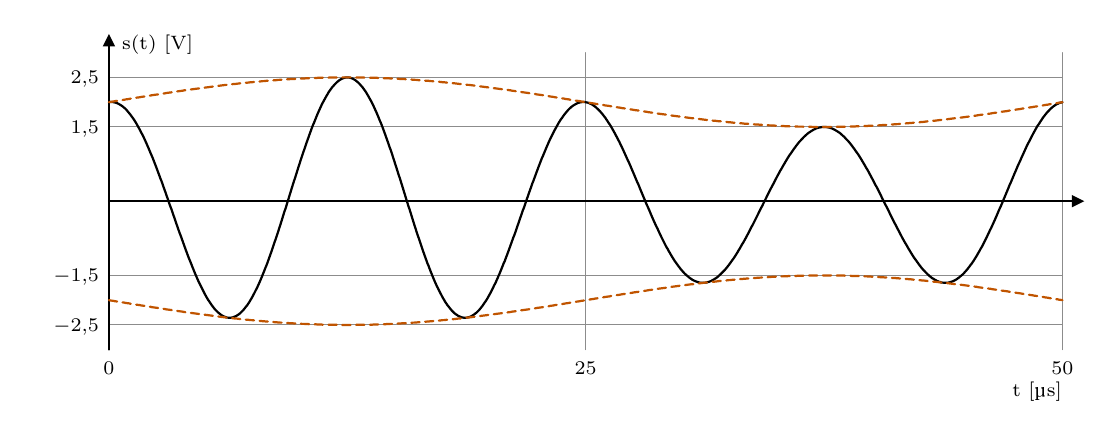
\begin{tikzpicture}[x=0.01985cm,y=-0.01985cm,line cap=round,line join=round]
\useasboundingbox (0,0) rectangle (680,240);
\path[draw=black!45,line width=0.35pt] (52,206) -- (52,16);
\path[draw=black!45,line width=0.35pt] (357,206) -- (357,16);
\path[draw=black!45,line width=0.35pt] (662,206) -- (662,16);
\path[draw=black!45,line width=0.35pt] (52,31.8) -- (662,31.8);
\path[draw=black!45,line width=0.35pt] (52,63.5) -- (662,63.5);
\path[draw=black!45,line width=0.35pt] (52,158.5) -- (662,158.5);
\path[draw=black!45,line width=0.35pt] (52,190.2) -- (662,190.2);
\path[draw=black,line width=0.7pt] (52,111) -- (670,111);
\path[fill=black,draw=none] (676,111) -- (668,107) -- (668,115) -- cycle;
\path[draw=black,line width=0.7pt] (52,206) -- (52,10);
\path[fill=black,draw=none] (52,4) -- (48,12) -- (56,12) -- cycle;
\node[anchor=base,inner sep=0pt,font=\scriptsize] at (52,222) {0};
\node[anchor=base,inner sep=0pt,font=\scriptsize] at (357,222) {25};
\node[anchor=base,inner sep=0pt,font=\scriptsize] at (662,222) {50};
\node[anchor=base east,inner sep=0pt,font=\scriptsize] at (46,35.8) {2,5};
\node[anchor=base east,inner sep=0pt,font=\scriptsize] at (46,67.5) {1,5};
\node[anchor=base east,inner sep=0pt,font=\scriptsize] at (46,162.5) {$-$1,5};
\node[anchor=base east,inner sep=0pt,font=\scriptsize] at (46,194.2) {$-$2,5};
\node[anchor=base east,inner sep=0pt,font=\scriptsize] at (662,236) {t [\textmu{}s]};
\node[anchor=base west,inner sep=0pt,font=\scriptsize] at (60,14) {s(t) [V]};
\path[draw=black,line width=0.8pt] (52,47.7) -- (52.5,47.6) -- (53,47.6) -- (53.5,47.5) -- (54,47.6) -- (54.5,47.6) -- (55.1,47.7) -- (55.6,47.8) -- (56.1,47.9) -- (56.6,48.1) -- (57.1,48.2) -- (57.6,48.5) -- (58.1,48.7) -- (58.6,49) -- (59.1,49.3) -- (59.6,49.6) -- (60.1,49.9) -- (60.6,50.3) -- (61.2,50.7) -- (61.7,51.2) -- (62.2,51.6) -- (62.7,52.1) -- (63.2,52.6) -- (63.7,53.2) -- (64.2,53.8) -- (64.7,54.4) -- (65.2,55) -- (65.7,55.6) -- (66.2,56.3) -- (66.7,57) -- (67.3,57.8) -- (67.8,58.5) -- (68.3,59.3) -- (68.8,60.1) -- (69.3,60.9) -- (69.8,61.8) -- (70.3,62.7) -- (70.8,63.6) -- (71.3,64.5) -- (71.8,65.4) -- (72.3,66.4) -- (72.8,67.4) -- (73.4,68.4) -- (73.9,69.5) -- (74.4,70.5) -- (74.9,71.6) -- (75.4,72.7) -- (75.9,73.8) -- (76.4,75) -- (76.9,76.1) -- (77.4,77.3) -- (77.9,78.5) -- (78.4,79.7) -- (78.9,80.9) -- (79.5,82.2) -- (80,83.4) -- (80.5,84.7) -- (81,86) -- (81.5,87.3) -- (82,88.6) -- (82.5,89.9) -- (83,91.3) -- (83.5,92.6) -- (84,94) -- (84.5,95.3) -- (85,96.7) -- (85.6,98.1) -- (86.1,99.5) -- (86.6,100.9) -- (87.1,102.4) -- (87.6,103.8) -- (88.1,105.2) -- (88.6,106.7) -- (89.1,108.1) -- (89.6,109.5) -- (90.1,111) -- (90.6,112.5) -- (91.1,113.9) -- (91.7,115.4) -- (92.2,116.8) -- (92.7,118.3) -- (93.2,119.8) -- (93.7,121.2) -- (94.2,122.7) -- (94.7,124.1) -- (95.2,125.6) -- (95.7,127) -- (96.2,128.5) -- (96.7,129.9) -- (97.2,131.4) -- (97.8,132.8) -- (98.3,134.2) -- (98.8,135.6) -- (99.3,137) -- (99.8,138.4) -- (100.3,139.8) -- (100.8,141.2) -- (101.3,142.6) -- (101.8,143.9) -- (102.3,145.3) -- (102.8,146.6) -- (103.3,147.9) -- (103.9,149.3) -- (104.4,150.5) -- (104.9,151.8) -- (105.4,153.1) -- (105.9,154.3) -- (106.4,155.6) -- (106.9,156.8) -- (107.4,158) -- (107.9,159.1) -- (108.4,160.3) -- (108.9,161.4) -- (109.4,162.6) -- (110,163.7) -- (110.5,164.7) -- (111,165.8) -- (111.5,166.8) -- (112,167.8) -- (112.5,168.8) -- (113,169.8) -- (113.5,170.7) -- (114,171.6) -- (114.5,172.5) -- (115,173.4) -- (115.5,174.2) -- (116.1,175) -- (116.6,175.8) -- (117.1,176.5) -- (117.6,177.3) -- (118.1,178) -- (118.6,178.6) -- (119.1,179.3) -- (119.6,179.9) -- (120.1,180.5) -- (120.6,181) -- (121.1,181.5) -- (121.6,182) -- (122.2,182.5) -- (122.7,182.9) -- (123.2,183.3) -- (123.7,183.7) -- (124.2,184) -- (124.7,184.3) -- (125.2,184.6) -- (125.7,184.8) -- (126.2,185) -- (126.7,185.2) -- (127.2,185.3) -- (127.7,185.5) -- (128.3,185.5) -- (128.8,185.6) -- (129.3,185.6) -- (129.8,185.6) -- (130.3,185.5) -- (130.8,185.4) -- (131.3,185.3) -- (131.8,185.1) -- (132.3,184.9) -- (132.8,184.7) -- (133.3,184.5) -- (133.8,184.2) -- (134.4,183.8) -- (134.9,183.5) -- (135.4,183.1) -- (135.9,182.7) -- (136.4,182.2) -- (136.9,181.7) -- (137.4,181.2) -- (137.9,180.7) -- (138.4,180.1) -- (138.9,179.5) -- (139.4,178.8) -- (139.9,178.2) -- (140.5,177.5) -- (141,176.7) -- (141.5,176) -- (142,175.2) -- (142.5,174.3) -- (143,173.5) -- (143.5,172.6) -- (144,171.7) -- (144.5,170.7) -- (145,169.8) -- (145.5,168.8) -- (146,167.8) -- (146.6,166.7) -- (147.1,165.6) -- (147.6,164.5) -- (148.1,163.4) -- (148.6,162.3) -- (149.1,161.1) -- (149.6,159.9) -- (150.1,158.7) -- (150.6,157.4) -- (151.1,156.2) -- (151.6,154.9) -- (152.1,153.6) -- (152.7,152.2) -- (153.2,150.9) -- (153.7,149.5) -- (154.2,148.1) -- (154.7,146.7) -- (155.2,145.3) -- (155.7,143.9) -- (156.2,142.4) -- (156.7,141) -- (157.2,139.5) -- (157.7,138) -- (158.2,136.5) -- (158.8,134.9) -- (159.3,133.4) -- (159.8,131.8) -- (160.3,130.3) -- (160.8,128.7) -- (161.3,127.1) -- (161.8,125.6) -- (162.3,124) -- (162.8,122.4) -- (163.3,120.7) -- (163.8,119.1) -- (164.3,117.5) -- (164.9,115.9) -- (165.4,114.3) -- (165.9,112.6) -- (166.4,111) -- (166.9,109.4) -- (167.4,107.7) -- (167.9,106.1) -- (168.4,104.5) -- (168.9,102.8) -- (169.4,101.2) -- (169.9,99.6) -- (170.4,98) -- (171,96.3) -- (171.5,94.7) -- (172,93.1) -- (172.5,91.5) -- (173,89.9) -- (173.5,88.3) -- (174,86.8) -- (174.5,85.2) -- (175,83.7) -- (175.5,82.1) -- (176,80.6) -- (176.5,79.1) -- (177.1,77.6) -- (177.6,76.1) -- (178.1,74.6) -- (178.6,73.1) -- (179.1,71.7) -- (179.6,70.3) -- (180.1,68.8) -- (180.6,67.5) -- (181.1,66.1) -- (181.6,64.7) -- (182.1,63.4) -- (182.6,62.1) -- (183.2,60.8) -- (183.7,59.5) -- (184.2,58.3) -- (184.7,57) -- (185.2,55.8) -- (185.7,54.6) -- (186.2,53.5) -- (186.7,52.4) -- (187.2,51.3) -- (187.7,50.2) -- (188.2,49.1) -- (188.7,48.1) -- (189.3,47.1) -- (189.8,46.1) -- (190.3,45.2) -- (190.8,44.3) -- (191.3,43.4) -- (191.8,42.6) -- (192.3,41.7) -- (192.8,40.9) -- (193.3,40.2) -- (193.8,39.5) -- (194.3,38.8) -- (194.8,38.1) -- (195.4,37.5) -- (195.9,36.9) -- (196.4,36.3) -- (196.9,35.8) -- (197.4,35.3) -- (197.9,34.8) -- (198.4,34.4) -- (198.9,34) -- (199.4,33.6) -- (199.9,33.3) -- (200.4,33) -- (200.9,32.7) -- (201.5,32.5) -- (202,32.3) -- (202.5,32.1) -- (203,32) -- (203.5,31.9) -- (204,31.9) -- (204.5,31.8) -- (205,31.9) -- (205.5,31.9) -- (206,32) -- (206.5,32.1) -- (207,32.3) -- (207.6,32.5) -- (208.1,32.7) -- (208.6,33) -- (209.1,33.3) -- (209.6,33.6) -- (210.1,34) -- (210.6,34.4) -- (211.1,34.8) -- (211.6,35.3) -- (212.1,35.8) -- (212.6,36.3) -- (213.1,36.9) -- (213.7,37.5) -- (214.2,38.1) -- (214.7,38.8) -- (215.2,39.5) -- (215.7,40.2) -- (216.2,40.9) -- (216.7,41.7) -- (217.2,42.6) -- (217.7,43.4) -- (218.2,44.3) -- (218.7,45.2) -- (219.2,46.1) -- (219.8,47.1) -- (220.3,48.1) -- (220.8,49.1) -- (221.3,50.2) -- (221.8,51.3) -- (222.3,52.4) -- (222.8,53.5) -- (223.3,54.6) -- (223.8,55.8) -- (224.3,57) -- (224.8,58.3) -- (225.3,59.5) -- (225.9,60.8) -- (226.4,62.1) -- (226.9,63.4) -- (227.4,64.7) -- (227.9,66.1) -- (228.4,67.5) -- (228.9,68.8) -- (229.4,70.3) -- (229.9,71.7) -- (230.4,73.1) -- (230.9,74.6) -- (231.4,76.1) -- (232,77.6) -- (232.5,79.1) -- (233,80.6) -- (233.5,82.1) -- (234,83.7) -- (234.5,85.2) -- (235,86.8) -- (235.5,88.3) -- (236,89.9) -- (236.5,91.5) -- (237,93.1) -- (237.5,94.7) -- (238.1,96.3) -- (238.6,98) -- (239.1,99.6) -- (239.6,101.2) -- (240.1,102.8) -- (240.6,104.5) -- (241.1,106.1) -- (241.6,107.7) -- (242.1,109.4) -- (242.6,111) -- (243.1,112.6) -- (243.6,114.3) -- (244.2,115.9) -- (244.7,117.5) -- (245.2,119.1) -- (245.7,120.7) -- (246.2,122.4) -- (246.7,124) -- (247.2,125.6) -- (247.7,127.1) -- (248.2,128.7) -- (248.7,130.3) -- (249.2,131.8) -- (249.7,133.4) -- (250.3,134.9) -- (250.8,136.5) -- (251.3,138) -- (251.8,139.5) -- (252.3,141) -- (252.8,142.4) -- (253.3,143.9) -- (253.8,145.3) -- (254.3,146.7) -- (254.8,148.1) -- (255.3,149.5) -- (255.8,150.9) -- (256.4,152.2) -- (256.9,153.6) -- (257.4,154.9) -- (257.9,156.2) -- (258.4,157.4) -- (258.9,158.7) -- (259.4,159.9) -- (259.9,161.1) -- (260.4,162.3) -- (260.9,163.4) -- (261.4,164.5) -- (261.9,165.6) -- (262.5,166.7) -- (263,167.8) -- (263.5,168.8) -- (264,169.8) -- (264.5,170.7) -- (265,171.7) -- (265.5,172.6) -- (266,173.5) -- (266.5,174.3) -- (267,175.2) -- (267.5,176) -- (268,176.7) -- (268.5,177.5) -- (269.1,178.2) -- (269.6,178.8) -- (270.1,179.5) -- (270.6,180.1) -- (271.1,180.7) -- (271.6,181.2) -- (272.1,181.7) -- (272.6,182.2) -- (273.1,182.7) -- (273.6,183.1) -- (274.1,183.5) -- (274.7,183.8) -- (275.2,184.2) -- (275.7,184.5) -- (276.2,184.7) -- (276.7,184.9) -- (277.2,185.1) -- (277.7,185.3) -- (278.2,185.4) -- (278.7,185.5) -- (279.2,185.6) -- (279.7,185.6) -- (280.2,185.6) -- (280.8,185.5) -- (281.3,185.5) -- (281.8,185.3) -- (282.3,185.2) -- (282.8,185) -- (283.3,184.8) -- (283.8,184.6) -- (284.3,184.3) -- (284.8,184) -- (285.3,183.7) -- (285.8,183.3) -- (286.3,182.9) -- (286.9,182.5) -- (287.4,182) -- (287.9,181.5) -- (288.4,181) -- (288.9,180.5) -- (289.4,179.9) -- (289.9,179.3) -- (290.4,178.6) -- (290.9,178) -- (291.4,177.3) -- (291.9,176.5) -- (292.4,175.8) -- (293,175) -- (293.5,174.2) -- (294,173.4) -- (294.5,172.5) -- (295,171.6) -- (295.5,170.7) -- (296,169.8) -- (296.5,168.8) -- (297,167.8) -- (297.5,166.8) -- (298,165.8) -- (298.5,164.7) -- (299.1,163.7) -- (299.6,162.6) -- (300.1,161.4) -- (300.6,160.3) -- (301.1,159.1) -- (301.6,158) -- (302.1,156.8) -- (302.6,155.6) -- (303.1,154.3) -- (303.6,153.1) -- (304.1,151.8) -- (304.6,150.5) -- (305.2,149.3) -- (305.7,147.9) -- (306.2,146.6) -- (306.7,145.3) -- (307.2,143.9) -- (307.7,142.6) -- (308.2,141.2) -- (308.7,139.8) -- (309.2,138.4) -- (309.7,137) -- (310.2,135.6) -- (310.7,134.2) -- (311.3,132.8) -- (311.8,131.4) -- (312.3,129.9) -- (312.8,128.5) -- (313.3,127) -- (313.8,125.6) -- (314.3,124.1) -- (314.8,122.7) -- (315.3,121.2) -- (315.8,119.8) -- (316.3,118.3) -- (316.8,116.8) -- (317.4,115.4) -- (317.9,113.9) -- (318.4,112.5) -- (318.9,111) -- (319.4,109.5) -- (319.9,108.1) -- (320.4,106.7) -- (320.9,105.2) -- (321.4,103.8) -- (321.9,102.4) -- (322.4,100.9) -- (322.9,99.5) -- (323.5,98.1) -- (324,96.7) -- (324.5,95.3) -- (325,94) -- (325.5,92.6) -- (326,91.3) -- (326.5,89.9) -- (327,88.6) -- (327.5,87.3) -- (328,86) -- (328.5,84.7) -- (329,83.4) -- (329.6,82.2) -- (330.1,80.9) -- (330.6,79.7) -- (331.1,78.5) -- (331.6,77.3) -- (332.1,76.1) -- (332.6,75) -- (333.1,73.8) -- (333.6,72.7) -- (334.1,71.6) -- (334.6,70.5) -- (335.1,69.5) -- (335.7,68.4) -- (336.2,67.4) -- (336.7,66.4) -- (337.2,65.4) -- (337.7,64.5) -- (338.2,63.6) -- (338.7,62.7) -- (339.2,61.8) -- (339.7,60.9) -- (340.2,60.1) -- (340.7,59.3) -- (341.2,58.5) -- (341.8,57.8) -- (342.3,57) -- (342.8,56.3) -- (343.3,55.6) -- (343.8,55) -- (344.3,54.4) -- (344.8,53.8) -- (345.3,53.2) -- (345.8,52.6) -- (346.3,52.1) -- (346.8,51.6) -- (347.3,51.2) -- (347.8,50.7) -- (348.4,50.3) -- (348.9,49.9) -- (349.4,49.6) -- (349.9,49.3) -- (350.4,49) -- (350.9,48.7) -- (351.4,48.5) -- (351.9,48.2) -- (352.4,48.1) -- (352.9,47.9) -- (353.4,47.8) -- (354,47.7) -- (354.5,47.6) -- (355,47.6) -- (355.5,47.5) -- (356,47.6) -- (356.5,47.6) -- (357,47.7) -- (357.5,47.8) -- (358,47.9) -- (358.5,48) -- (359,48.2) -- (359.5,48.4) -- (360.1,48.7) -- (360.6,48.9) -- (361.1,49.2) -- (361.6,49.5) -- (362.1,49.9) -- (362.6,50.2) -- (363.1,50.6) -- (363.6,51) -- (364.1,51.5) -- (364.6,51.9) -- (365.1,52.4) -- (365.6,53) -- (366.2,53.5) -- (366.7,54.1) -- (367.2,54.7) -- (367.7,55.3) -- (368.2,55.9) -- (368.7,56.6) -- (369.2,57.2) -- (369.7,57.9) -- (370.2,58.7) -- (370.7,59.4) -- (371.2,60.2) -- (371.7,61) -- (372.3,61.8) -- (372.8,62.6) -- (373.3,63.4) -- (373.8,64.3) -- (374.3,65.2) -- (374.8,66.1) -- (375.3,67) -- (375.8,67.9) -- (376.3,68.9) -- (376.8,69.8) -- (377.3,70.8) -- (377.8,71.8) -- (378.4,72.8) -- (378.9,73.9) -- (379.4,74.9) -- (379.9,75.9) -- (380.4,77) -- (380.9,78.1) -- (381.4,79.2) -- (381.9,80.3) -- (382.4,81.4) -- (382.9,82.5) -- (383.4,83.6) -- (383.9,84.8) -- (384.5,85.9) -- (385,87.1) -- (385.5,88.2) -- (386,89.4) -- (386.5,90.6) -- (387,91.8) -- (387.5,92.9) -- (388,94.1) -- (388.5,95.3) -- (389,96.5) -- (389.5,97.7) -- (390,98.9) -- (390.6,100.1) -- (391.1,101.3) -- (391.6,102.6) -- (392.1,103.8) -- (392.6,105) -- (393.1,106.2) -- (393.6,107.4) -- (394.1,108.6) -- (394.6,109.8) -- (395.1,111) -- (395.6,112.2) -- (396.1,113.4) -- (396.7,114.6) -- (397.2,115.8) -- (397.7,116.9) -- (398.2,118.1) -- (398.7,119.3) -- (399.2,120.5) -- (399.7,121.6) -- (400.2,122.8) -- (400.7,123.9) -- (401.2,125) -- (401.7,126.1) -- (402.2,127.2) -- (402.8,128.3) -- (403.3,129.4) -- (403.8,130.5) -- (404.3,131.6) -- (404.8,132.6) -- (405.3,133.7) -- (405.8,134.7) -- (406.3,135.7) -- (406.8,136.7) -- (407.3,137.7) -- (407.8,138.7) -- (408.3,139.7) -- (408.8,140.6) -- (409.4,141.5) -- (409.9,142.5) -- (410.4,143.4) -- (410.9,144.2) -- (411.4,145.1) -- (411.9,146) -- (412.4,146.8) -- (412.9,147.6) -- (413.4,148.4) -- (413.9,149.2) -- (414.4,149.9) -- (415,150.7) -- (415.5,151.4) -- (416,152.1) -- (416.5,152.8) -- (417,153.4) -- (417.5,154.1) -- (418,154.7) -- (418.5,155.3) -- (419,155.9) -- (419.5,156.4) -- (420,157) -- (420.5,157.5) -- (421.1,158) -- (421.6,158.5) -- (422.1,158.9) -- (422.6,159.3) -- (423.1,159.8) -- (423.6,160.1) -- (424.1,160.5) -- (424.6,160.8) -- (425.1,161.2) -- (425.6,161.5) -- (426.1,161.7) -- (426.6,162) -- (427.2,162.2) -- (427.7,162.4) -- (428.2,162.6) -- (428.7,162.7) -- (429.2,162.9) -- (429.7,163) -- (430.2,163.1) -- (430.7,163.1) -- (431.2,163.2) -- (431.7,163.2) -- (432.2,163.2) -- (432.7,163.2) -- (433.3,163.1) -- (433.8,163.1) -- (434.3,163) -- (434.8,162.9) -- (435.3,162.7) -- (435.8,162.6) -- (436.3,162.4) -- (436.8,162.2) -- (437.3,162) -- (437.8,161.7) -- (438.3,161.4) -- (438.8,161.2) -- (439.4,160.8) -- (439.9,160.5) -- (440.4,160.2) -- (440.9,159.8) -- (441.4,159.4) -- (441.9,159) -- (442.4,158.5) -- (442.9,158.1) -- (443.4,157.6) -- (443.9,157.1) -- (444.4,156.6) -- (444.9,156.1) -- (445.5,155.5) -- (446,155) -- (446.5,154.4) -- (447,153.8) -- (447.5,153.2) -- (448,152.5) -- (448.5,151.9) -- (449,151.2) -- (449.5,150.5) -- (450,149.8) -- (450.5,149.1) -- (451,148.4) -- (451.6,147.6) -- (452.1,146.9) -- (452.6,146.1) -- (453.1,145.3) -- (453.6,144.5) -- (454.1,143.7) -- (454.6,142.8) -- (455.1,142) -- (455.6,141.2) -- (456.1,140.3) -- (456.6,139.4) -- (457.1,138.5) -- (457.7,137.6) -- (458.2,136.7) -- (458.7,135.8) -- (459.2,134.9) -- (459.7,134) -- (460.2,133) -- (460.7,132.1) -- (461.2,131.1) -- (461.7,130.1) -- (462.2,129.2) -- (462.7,128.2) -- (463.2,127.2) -- (463.8,126.2) -- (464.3,125.2) -- (464.8,124.2) -- (465.3,123.2) -- (465.8,122.2) -- (466.3,121.2) -- (466.8,120.2) -- (467.3,119.2) -- (467.8,118.1) -- (468.3,117.1) -- (468.8,116.1) -- (469.3,115.1) -- (469.9,114.1) -- (470.4,113) -- (470.9,112) -- (471.4,111) -- (471.9,110) -- (472.4,109) -- (472.9,107.9) -- (473.4,106.9) -- (473.9,105.9) -- (474.4,104.9) -- (474.9,103.9) -- (475.4,102.9) -- (476,101.9) -- (476.5,100.9) -- (477,100) -- (477.5,99) -- (478,98) -- (478.5,97) -- (479,96.1) -- (479.5,95.1) -- (480,94.2) -- (480.5,93.3) -- (481,92.3) -- (481.5,91.4) -- (482.1,90.5) -- (482.6,89.6) -- (483.1,88.7) -- (483.6,87.8) -- (484.1,87) -- (484.6,86.1) -- (485.1,85.3) -- (485.6,84.4) -- (486.1,83.6) -- (486.6,82.8) -- (487.1,82) -- (487.6,81.2) -- (488.2,80.5) -- (488.7,79.7) -- (489.2,79) -- (489.7,78.3) -- (490.2,77.5) -- (490.7,76.9) -- (491.2,76.2) -- (491.7,75.5) -- (492.2,74.9) -- (492.7,74.2) -- (493.2,73.6) -- (493.7,73) -- (494.3,72.4) -- (494.8,71.8) -- (495.3,71.3) -- (495.8,70.8) -- (496.3,70.2) -- (496.8,69.7) -- (497.3,69.3) -- (497.8,68.8) -- (498.3,68.4) -- (498.8,67.9) -- (499.3,67.5) -- (499.8,67.1) -- (500.4,66.8) -- (500.9,66.4) -- (501.4,66.1) -- (501.9,65.8) -- (502.4,65.5) -- (502.9,65.2) -- (503.4,65) -- (503.9,64.7) -- (504.4,64.5) -- (504.9,64.3) -- (505.4,64.2) -- (505.9,64) -- (506.5,63.9) -- (507,63.8) -- (507.5,63.7) -- (508,63.6) -- (508.5,63.5) -- (509,63.5) -- (509.5,63.5) -- (510,63.5) -- (510.5,63.5) -- (511,63.6) -- (511.5,63.7) -- (512,63.8) -- (512.6,63.9) -- (513.1,64) -- (513.6,64.2) -- (514.1,64.3) -- (514.6,64.5) -- (515.1,64.7) -- (515.6,65) -- (516.1,65.2) -- (516.6,65.5) -- (517.1,65.8) -- (517.6,66.1) -- (518.1,66.4) -- (518.7,66.8) -- (519.2,67.1) -- (519.7,67.5) -- (520.2,67.9) -- (520.7,68.4) -- (521.2,68.8) -- (521.7,69.3) -- (522.2,69.7) -- (522.7,70.2) -- (523.2,70.8) -- (523.7,71.3) -- (524.2,71.8) -- (524.8,72.4) -- (525.3,73) -- (525.8,73.6) -- (526.3,74.2) -- (526.8,74.9) -- (527.3,75.5) -- (527.8,76.2) -- (528.3,76.9) -- (528.8,77.5) -- (529.3,78.3) -- (529.8,79) -- (530.3,79.7) -- (530.9,80.5) -- (531.4,81.2) -- (531.9,82) -- (532.4,82.8) -- (532.9,83.6) -- (533.4,84.4) -- (533.9,85.3) -- (534.4,86.1) -- (534.9,87) -- (535.4,87.8) -- (535.9,88.7) -- (536.4,89.6) -- (537,90.5) -- (537.5,91.4) -- (538,92.3) -- (538.5,93.3) -- (539,94.2) -- (539.5,95.1) -- (540,96.1) -- (540.5,97) -- (541,98) -- (541.5,99) -- (542,100) -- (542.5,100.9) -- (543.1,101.9) -- (543.6,102.9) -- (544.1,103.9) -- (544.6,104.9) -- (545.1,105.9) -- (545.6,106.9) -- (546.1,107.9) -- (546.6,109) -- (547.1,110) -- (547.6,111) -- (548.1,112) -- (548.6,113) -- (549.2,114.1) -- (549.7,115.1) -- (550.2,116.1) -- (550.7,117.1) -- (551.2,118.1) -- (551.7,119.2) -- (552.2,120.2) -- (552.7,121.2) -- (553.2,122.2) -- (553.7,123.2) -- (554.2,124.2) -- (554.7,125.2) -- (555.3,126.2) -- (555.8,127.2) -- (556.3,128.2) -- (556.8,129.2) -- (557.3,130.1) -- (557.8,131.1) -- (558.3,132.1) -- (558.8,133) -- (559.3,134) -- (559.8,134.9) -- (560.3,135.8) -- (560.8,136.7) -- (561.3,137.6) -- (561.9,138.5) -- (562.4,139.4) -- (562.9,140.3) -- (563.4,141.2) -- (563.9,142) -- (564.4,142.8) -- (564.9,143.7) -- (565.4,144.5) -- (565.9,145.3) -- (566.4,146.1) -- (566.9,146.9) -- (567.4,147.6) -- (568,148.4) -- (568.5,149.1) -- (569,149.8) -- (569.5,150.5) -- (570,151.2) -- (570.5,151.9) -- (571,152.5) -- (571.5,153.2) -- (572,153.8) -- (572.5,154.4) -- (573,155) -- (573.6,155.5) -- (574.1,156.1) -- (574.6,156.6) -- (575.1,157.1) -- (575.6,157.6) -- (576.1,158.1) -- (576.6,158.5) -- (577.1,159) -- (577.6,159.4) -- (578.1,159.8) -- (578.6,160.2) -- (579.1,160.5) -- (579.7,160.8) -- (580.2,161.2) -- (580.7,161.4) -- (581.2,161.7) -- (581.7,162) -- (582.2,162.2) -- (582.7,162.4) -- (583.2,162.6) -- (583.7,162.7) -- (584.2,162.9) -- (584.7,163) -- (585.2,163.1) -- (585.8,163.1) -- (586.3,163.2) -- (586.8,163.2) -- (587.3,163.2) -- (587.8,163.2) -- (588.3,163.1) -- (588.8,163.1) -- (589.3,163) -- (589.8,162.9) -- (590.3,162.7) -- (590.8,162.6) -- (591.3,162.4) -- (591.9,162.2) -- (592.4,162) -- (592.9,161.7) -- (593.4,161.5) -- (593.9,161.2) -- (594.4,160.8) -- (594.9,160.5) -- (595.4,160.1) -- (595.9,159.8) -- (596.4,159.3) -- (596.9,158.9) -- (597.4,158.5) -- (598,158) -- (598.5,157.5) -- (599,157) -- (599.5,156.4) -- (600,155.9) -- (600.5,155.3) -- (601,154.7) -- (601.5,154.1) -- (602,153.4) -- (602.5,152.8) -- (603,152.1) -- (603.5,151.4) -- (604.1,150.7) -- (604.6,149.9) -- (605.1,149.2) -- (605.6,148.4) -- (606.1,147.6) -- (606.6,146.8) -- (607.1,146) -- (607.6,145.1) -- (608.1,144.2) -- (608.6,143.4) -- (609.1,142.5) -- (609.6,141.5) -- (610.2,140.6) -- (610.7,139.7) -- (611.2,138.7) -- (611.7,137.7) -- (612.2,136.7) -- (612.7,135.7) -- (613.2,134.7) -- (613.7,133.7) -- (614.2,132.6) -- (614.7,131.6) -- (615.2,130.5) -- (615.7,129.4) -- (616.3,128.3) -- (616.8,127.2) -- (617.3,126.1) -- (617.8,125) -- (618.3,123.9) -- (618.8,122.8) -- (619.3,121.6) -- (619.8,120.5) -- (620.3,119.3) -- (620.8,118.1) -- (621.3,116.9) -- (621.8,115.8) -- (622.4,114.6) -- (622.9,113.4) -- (623.4,112.2) -- (623.9,111) -- (624.4,109.8) -- (624.9,108.6) -- (625.4,107.4) -- (625.9,106.2) -- (626.4,105) -- (626.9,103.8) -- (627.4,102.6) -- (627.9,101.3) -- (628.4,100.1) -- (629,98.9) -- (629.5,97.7) -- (630,96.5) -- (630.5,95.3) -- (631,94.1) -- (631.5,92.9) -- (632,91.8) -- (632.5,90.6) -- (633,89.4) -- (633.5,88.2) -- (634,87.1) -- (634.6,85.9) -- (635.1,84.8) -- (635.6,83.6) -- (636.1,82.5) -- (636.6,81.4) -- (637.1,80.3) -- (637.6,79.2) -- (638.1,78.1) -- (638.6,77) -- (639.1,75.9) -- (639.6,74.9) -- (640.1,73.9) -- (640.7,72.8) -- (641.2,71.8) -- (641.7,70.8) -- (642.2,69.8) -- (642.7,68.9) -- (643.2,67.9) -- (643.7,67) -- (644.2,66.1) -- (644.7,65.2) -- (645.2,64.3) -- (645.7,63.4) -- (646.2,62.6) -- (646.8,61.8) -- (647.3,61) -- (647.8,60.2) -- (648.3,59.4) -- (648.8,58.7) -- (649.3,57.9) -- (649.8,57.2) -- (650.3,56.6) -- (650.8,55.9) -- (651.3,55.3) -- (651.8,54.7) -- (652.3,54.1) -- (652.9,53.5) -- (653.4,53) -- (653.9,52.4) -- (654.4,51.9) -- (654.9,51.5) -- (655.4,51) -- (655.9,50.6) -- (656.4,50.2) -- (656.9,49.9) -- (657.4,49.5) -- (657.9,49.2) -- (658.4,48.9) -- (659,48.7) -- (659.5,48.4) -- (660,48.2) -- (660.5,48) -- (661,47.9) -- (661.5,47.8) -- (662,47.7);
\path[draw=cB,line width=0.8pt,dash pattern=on 3pt off 2pt] (52,47.7) -- (52.8,47.5) -- (53.5,47.4) -- (54.3,47.3) -- (55.1,47.2) -- (55.8,47) -- (56.6,46.9) -- (57.3,46.8) -- (58.1,46.7) -- (58.9,46.5) -- (59.6,46.4) -- (60.4,46.3) -- (61.2,46.2) -- (61.9,46.1) -- (62.7,45.9) -- (63.4,45.8) -- (64.2,45.7) -- (65,45.6) -- (65.7,45.4) -- (66.5,45.3) -- (67.3,45.2) -- (68,45.1) -- (68.8,44.9) -- (69.5,44.8) -- (70.3,44.7) -- (71.1,44.6) -- (71.8,44.5) -- (72.6,44.3) -- (73.4,44.2) -- (74.1,44.1) -- (74.9,44) -- (75.6,43.8) -- (76.4,43.7) -- (77.2,43.6) -- (77.9,43.5) -- (78.7,43.4) -- (79.5,43.2) -- (80.2,43.1) -- (81,43) -- (81.7,42.9) -- (82.5,42.8) -- (83.3,42.7) -- (84,42.5) -- (84.8,42.4) -- (85.6,42.3) -- (86.3,42.2) -- (87.1,42.1) -- (87.8,42) -- (88.6,41.8) -- (89.4,41.7) -- (90.1,41.6) -- (90.9,41.5) -- (91.7,41.4) -- (92.4,41.3) -- (93.2,41.2) -- (93.9,41) -- (94.7,40.9) -- (95.5,40.8) -- (96.2,40.7) -- (97,40.6) -- (97.8,40.5) -- (98.5,40.4) -- (99.3,40.3) -- (100,40.1) -- (100.8,40) -- (101.6,39.9) -- (102.3,39.8) -- (103.1,39.7) -- (103.9,39.6) -- (104.6,39.5) -- (105.4,39.4) -- (106.1,39.3) -- (106.9,39.2) -- (107.7,39.1) -- (108.4,39) -- (109.2,38.9) -- (110,38.8) -- (110.7,38.7) -- (111.5,38.6) -- (112.2,38.5) -- (113,38.4) -- (113.8,38.3) -- (114.5,38.2) -- (115.3,38.1) -- (116.1,38) -- (116.8,37.9) -- (117.6,37.8) -- (118.3,37.7) -- (119.1,37.6) -- (119.9,37.5) -- (120.6,37.4) -- (121.4,37.3) -- (122.2,37.2) -- (122.9,37.1) -- (123.7,37) -- (124.4,36.9) -- (125.2,36.8) -- (126,36.7) -- (126.7,36.6) -- (127.5,36.6) -- (128.3,36.5) -- (129,36.4) -- (129.8,36.3) -- (130.5,36.2) -- (131.3,36.1) -- (132.1,36) -- (132.8,36) -- (133.6,35.9) -- (134.4,35.8) -- (135.1,35.7) -- (135.9,35.6) -- (136.6,35.5) -- (137.4,35.5) -- (138.2,35.4) -- (138.9,35.3) -- (139.7,35.2) -- (140.5,35.2) -- (141.2,35.1) -- (142,35) -- (142.7,34.9) -- (143.5,34.9) -- (144.3,34.8) -- (145,34.7) -- (145.8,34.6) -- (146.6,34.6) -- (147.3,34.5) -- (148.1,34.4) -- (148.8,34.4) -- (149.6,34.3) -- (150.4,34.2) -- (151.1,34.2) -- (151.9,34.1) -- (152.7,34) -- (153.4,34) -- (154.2,33.9) -- (154.9,33.9) -- (155.7,33.8) -- (156.5,33.7) -- (157.2,33.7) -- (158,33.6) -- (158.8,33.6) -- (159.5,33.5) -- (160.3,33.4) -- (161,33.4) -- (161.8,33.3) -- (162.6,33.3) -- (163.3,33.2) -- (164.1,33.2) -- (164.9,33.1) -- (165.6,33.1) -- (166.4,33) -- (167.1,33) -- (167.9,32.9) -- (168.7,32.9) -- (169.4,32.9) -- (170.2,32.8) -- (171,32.8) -- (171.7,32.7) -- (172.5,32.7) -- (173.2,32.6) -- (174,32.6) -- (174.8,32.6) -- (175.5,32.5) -- (176.3,32.5) -- (177.1,32.5) -- (177.8,32.4) -- (178.6,32.4) -- (179.3,32.4) -- (180.1,32.3) -- (180.9,32.3) -- (181.6,32.3) -- (182.4,32.2) -- (183.2,32.2) -- (183.9,32.2) -- (184.7,32.2) -- (185.4,32.1) -- (186.2,32.1) -- (187,32.1) -- (187.7,32.1) -- (188.5,32) -- (189.3,32) -- (190,32) -- (190.8,32) -- (191.5,32) -- (192.3,32) -- (193.1,31.9) -- (193.8,31.9) -- (194.6,31.9) -- (195.4,31.9) -- (196.1,31.9) -- (196.9,31.9) -- (197.6,31.9) -- (198.4,31.9) -- (199.2,31.9) -- (199.9,31.9) -- (200.7,31.8) -- (201.5,31.8) -- (202.2,31.8) -- (203,31.8) -- (203.7,31.8) -- (204.5,31.8) -- (205.3,31.8) -- (206,31.8) -- (206.8,31.8) -- (207.6,31.8) -- (208.3,31.8) -- (209.1,31.9) -- (209.8,31.9) -- (210.6,31.9) -- (211.4,31.9) -- (212.1,31.9) -- (212.9,31.9) -- (213.7,31.9) -- (214.4,31.9) -- (215.2,31.9) -- (215.9,31.9) -- (216.7,32) -- (217.5,32) -- (218.2,32) -- (219,32) -- (219.8,32) -- (220.5,32) -- (221.3,32.1) -- (222,32.1) -- (222.8,32.1) -- (223.6,32.1) -- (224.3,32.2) -- (225.1,32.2) -- (225.9,32.2) -- (226.6,32.2) -- (227.4,32.3) -- (228.1,32.3) -- (228.9,32.3) -- (229.7,32.4) -- (230.4,32.4) -- (231.2,32.4) -- (232,32.5) -- (232.7,32.5) -- (233.5,32.5) -- (234.2,32.6) -- (235,32.6) -- (235.8,32.6) -- (236.5,32.7) -- (237.3,32.7) -- (238.1,32.8) -- (238.8,32.8) -- (239.6,32.9) -- (240.3,32.9) -- (241.1,32.9) -- (241.9,33) -- (242.6,33) -- (243.4,33.1) -- (244.2,33.1) -- (244.9,33.2) -- (245.7,33.2) -- (246.4,33.3) -- (247.2,33.3) -- (248,33.4) -- (248.7,33.4) -- (249.5,33.5) -- (250.3,33.6) -- (251,33.6) -- (251.8,33.7) -- (252.5,33.7) -- (253.3,33.8) -- (254.1,33.9) -- (254.8,33.9) -- (255.6,34) -- (256.4,34) -- (257.1,34.1) -- (257.9,34.2) -- (258.6,34.2) -- (259.4,34.3) -- (260.2,34.4) -- (260.9,34.4) -- (261.7,34.5) -- (262.5,34.6) -- (263.2,34.6) -- (264,34.7) -- (264.7,34.8) -- (265.5,34.9) -- (266.3,34.9) -- (267,35) -- (267.8,35.1) -- (268.5,35.2) -- (269.3,35.2) -- (270.1,35.3) -- (270.8,35.4) -- (271.6,35.5) -- (272.4,35.5) -- (273.1,35.6) -- (273.9,35.7) -- (274.7,35.8) -- (275.4,35.9) -- (276.2,36) -- (276.9,36) -- (277.7,36.1) -- (278.5,36.2) -- (279.2,36.3) -- (280,36.4) -- (280.8,36.5) -- (281.5,36.6) -- (282.3,36.6) -- (283,36.7) -- (283.8,36.8) -- (284.6,36.9) -- (285.3,37) -- (286.1,37.1) -- (286.9,37.2) -- (287.6,37.3) -- (288.4,37.4) -- (289.1,37.5) -- (289.9,37.6) -- (290.7,37.7) -- (291.4,37.8) -- (292.2,37.9) -- (293,38) -- (293.7,38.1) -- (294.5,38.2) -- (295.2,38.3) -- (296,38.4) -- (296.8,38.5) -- (297.5,38.6) -- (298.3,38.7) -- (299.1,38.8) -- (299.8,38.9) -- (300.6,39) -- (301.3,39.1) -- (302.1,39.2) -- (302.9,39.3) -- (303.6,39.4) -- (304.4,39.5) -- (305.2,39.6) -- (305.9,39.7) -- (306.7,39.8) -- (307.4,39.9) -- (308.2,40) -- (309,40.1) -- (309.7,40.3) -- (310.5,40.4) -- (311.3,40.5) -- (312,40.6) -- (312.8,40.7) -- (313.5,40.8) -- (314.3,40.9) -- (315.1,41) -- (315.8,41.2) -- (316.6,41.3) -- (317.4,41.4) -- (318.1,41.5) -- (318.9,41.6) -- (319.6,41.7) -- (320.4,41.8) -- (321.2,42) -- (321.9,42.1) -- (322.7,42.2) -- (323.5,42.3) -- (324.2,42.4) -- (325,42.5) -- (325.7,42.7) -- (326.5,42.8) -- (327.3,42.9) -- (328,43) -- (328.8,43.1) -- (329.6,43.2) -- (330.3,43.4) -- (331.1,43.5) -- (331.8,43.6) -- (332.6,43.7) -- (333.4,43.8) -- (334.1,44) -- (334.9,44.1) -- (335.7,44.2) -- (336.4,44.3) -- (337.2,44.5) -- (337.9,44.6) -- (338.7,44.7) -- (339.5,44.8) -- (340.2,44.9) -- (341,45.1) -- (341.8,45.2) -- (342.5,45.3) -- (343.3,45.4) -- (344,45.6) -- (344.8,45.7) -- (345.6,45.8) -- (346.3,45.9) -- (347.1,46.1) -- (347.8,46.2) -- (348.6,46.3) -- (349.4,46.4) -- (350.1,46.5) -- (350.9,46.7) -- (351.7,46.8) -- (352.4,46.9) -- (353.2,47) -- (354,47.2) -- (354.7,47.3) -- (355.5,47.4) -- (356.2,47.5) -- (357,47.7) -- (357.8,47.8) -- (358.5,47.9) -- (359.3,48) -- (360.1,48.2) -- (360.8,48.3) -- (361.6,48.4) -- (362.3,48.5) -- (363.1,48.7) -- (363.9,48.8) -- (364.6,48.9) -- (365.4,49) -- (366.2,49.2) -- (366.9,49.3) -- (367.7,49.4) -- (368.4,49.5) -- (369.2,49.7) -- (370,49.8) -- (370.7,49.9) -- (371.5,50) -- (372.3,50.1) -- (373,50.3) -- (373.8,50.4) -- (374.5,50.5) -- (375.3,50.6) -- (376.1,50.8) -- (376.8,50.9) -- (377.6,51) -- (378.4,51.1) -- (379.1,51.2) -- (379.9,51.4) -- (380.6,51.5) -- (381.4,51.6) -- (382.2,51.7) -- (382.9,51.8) -- (383.7,52) -- (384.5,52.1) -- (385.2,52.2) -- (386,52.3) -- (386.7,52.4) -- (387.5,52.6) -- (388.3,52.7) -- (389,52.8) -- (389.8,52.9) -- (390.6,53) -- (391.3,53.1) -- (392.1,53.3) -- (392.8,53.4) -- (393.6,53.5) -- (394.4,53.6) -- (395.1,53.7) -- (395.9,53.8) -- (396.7,54) -- (397.4,54.1) -- (398.2,54.2) -- (398.9,54.3) -- (399.7,54.4) -- (400.5,54.5) -- (401.2,54.6) -- (402,54.7) -- (402.8,54.9) -- (403.5,55) -- (404.3,55.1) -- (405,55.2) -- (405.8,55.3) -- (406.6,55.4) -- (407.3,55.5) -- (408.1,55.6) -- (408.8,55.7) -- (409.6,55.8) -- (410.4,55.9) -- (411.1,56) -- (411.9,56.2) -- (412.7,56.3) -- (413.4,56.4) -- (414.2,56.5) -- (415,56.6) -- (415.7,56.7) -- (416.5,56.8) -- (417.2,56.9) -- (418,57) -- (418.8,57.1) -- (419.5,57.2) -- (420.3,57.3) -- (421.1,57.4) -- (421.8,57.5) -- (422.6,57.6) -- (423.3,57.7) -- (424.1,57.8) -- (424.9,57.9) -- (425.6,57.9) -- (426.4,58) -- (427.2,58.1) -- (427.9,58.2) -- (428.7,58.3) -- (429.4,58.4) -- (430.2,58.5) -- (431,58.6) -- (431.7,58.7) -- (432.5,58.8) -- (433.3,58.9) -- (434,59) -- (434.8,59) -- (435.5,59.1) -- (436.3,59.2) -- (437.1,59.3) -- (437.8,59.4) -- (438.6,59.5) -- (439.4,59.5) -- (440.1,59.6) -- (440.9,59.7) -- (441.6,59.8) -- (442.4,59.9) -- (443.2,59.9) -- (443.9,60) -- (444.7,60.1) -- (445.5,60.2) -- (446.2,60.3) -- (447,60.3) -- (447.7,60.4) -- (448.5,60.5) -- (449.3,60.5) -- (450,60.6) -- (450.8,60.7) -- (451.6,60.8) -- (452.3,60.8) -- (453.1,60.9) -- (453.8,61) -- (454.6,61) -- (455.4,61.1) -- (456.1,61.2) -- (456.9,61.2) -- (457.7,61.3) -- (458.4,61.4) -- (459.2,61.4) -- (459.9,61.5) -- (460.7,61.5) -- (461.5,61.6) -- (462.2,61.7) -- (463,61.7) -- (463.8,61.8) -- (464.5,61.8) -- (465.3,61.9) -- (466,61.9) -- (466.8,62) -- (467.6,62) -- (468.3,62.1) -- (469.1,62.1) -- (469.9,62.2) -- (470.6,62.2) -- (471.4,62.3) -- (472.1,62.3) -- (472.9,62.4) -- (473.7,62.4) -- (474.4,62.5) -- (475.2,62.5) -- (476,62.6) -- (476.7,62.6) -- (477.5,62.6) -- (478.2,62.7) -- (479,62.7) -- (479.8,62.8) -- (480.5,62.8) -- (481.3,62.8) -- (482.1,62.9) -- (482.8,62.9) -- (483.6,62.9) -- (484.3,63) -- (485.1,63) -- (485.9,63) -- (486.6,63.1) -- (487.4,63.1) -- (488.2,63.1) -- (488.9,63.1) -- (489.7,63.2) -- (490.4,63.2) -- (491.2,63.2) -- (492,63.2) -- (492.7,63.3) -- (493.5,63.3) -- (494.3,63.3) -- (495,63.3) -- (495.8,63.3) -- (496.5,63.4) -- (497.3,63.4) -- (498.1,63.4) -- (498.8,63.4) -- (499.6,63.4) -- (500.4,63.4) -- (501.1,63.4) -- (501.9,63.5) -- (502.6,63.5) -- (503.4,63.5) -- (504.2,63.5) -- (504.9,63.5) -- (505.7,63.5) -- (506.5,63.5) -- (507.2,63.5) -- (508,63.5) -- (508.7,63.5) -- (509.5,63.5) -- (510.3,63.5) -- (511,63.5) -- (511.8,63.5) -- (512.6,63.5) -- (513.3,63.5) -- (514.1,63.5) -- (514.8,63.5) -- (515.6,63.5) -- (516.4,63.5) -- (517.1,63.5) -- (517.9,63.4) -- (518.7,63.4) -- (519.4,63.4) -- (520.2,63.4) -- (520.9,63.4) -- (521.7,63.4) -- (522.5,63.4) -- (523.2,63.3) -- (524,63.3) -- (524.8,63.3) -- (525.5,63.3) -- (526.3,63.3) -- (527,63.2) -- (527.8,63.2) -- (528.6,63.2) -- (529.3,63.2) -- (530.1,63.1) -- (530.9,63.1) -- (531.6,63.1) -- (532.4,63.1) -- (533.1,63) -- (533.9,63) -- (534.7,63) -- (535.4,62.9) -- (536.2,62.9) -- (537,62.9) -- (537.7,62.8) -- (538.5,62.8) -- (539.2,62.8) -- (540,62.7) -- (540.8,62.7) -- (541.5,62.6) -- (542.3,62.6) -- (543.1,62.6) -- (543.8,62.5) -- (544.6,62.5) -- (545.3,62.4) -- (546.1,62.4) -- (546.9,62.3) -- (547.6,62.3) -- (548.4,62.2) -- (549.2,62.2) -- (549.9,62.1) -- (550.7,62.1) -- (551.4,62) -- (552.2,62) -- (553,61.9) -- (553.7,61.9) -- (554.5,61.8) -- (555.3,61.8) -- (556,61.7) -- (556.8,61.7) -- (557.5,61.6) -- (558.3,61.5) -- (559.1,61.5) -- (559.8,61.4) -- (560.6,61.4) -- (561.3,61.3) -- (562.1,61.2) -- (562.9,61.2) -- (563.6,61.1) -- (564.4,61) -- (565.2,61) -- (565.9,60.9) -- (566.7,60.8) -- (567.4,60.8) -- (568.2,60.7) -- (569,60.6) -- (569.7,60.5) -- (570.5,60.5) -- (571.3,60.4) -- (572,60.3) -- (572.8,60.3) -- (573.6,60.2) -- (574.3,60.1) -- (575.1,60) -- (575.8,59.9) -- (576.6,59.9) -- (577.4,59.8) -- (578.1,59.7) -- (578.9,59.6) -- (579.7,59.5) -- (580.4,59.5) -- (581.2,59.4) -- (581.9,59.3) -- (582.7,59.2) -- (583.5,59.1) -- (584.2,59) -- (585,59) -- (585.8,58.9) -- (586.5,58.8) -- (587.3,58.7) -- (588,58.6) -- (588.8,58.5) -- (589.6,58.4) -- (590.3,58.3) -- (591.1,58.2) -- (591.9,58.1) -- (592.6,58) -- (593.4,57.9) -- (594.1,57.9) -- (594.9,57.8) -- (595.7,57.7) -- (596.4,57.6) -- (597.2,57.5) -- (598,57.4) -- (598.7,57.3) -- (599.5,57.2) -- (600.2,57.1) -- (601,57) -- (601.8,56.9) -- (602.5,56.8) -- (603.3,56.7) -- (604.1,56.6) -- (604.8,56.5) -- (605.6,56.4) -- (606.3,56.3) -- (607.1,56.2) -- (607.9,56) -- (608.6,55.9) -- (609.4,55.8) -- (610.2,55.7) -- (610.9,55.6) -- (611.7,55.5) -- (612.4,55.4) -- (613.2,55.3) -- (614,55.2) -- (614.7,55.1) -- (615.5,55) -- (616.3,54.9) -- (617,54.7) -- (617.8,54.6) -- (618.5,54.5) -- (619.3,54.4) -- (620.1,54.3) -- (620.8,54.2) -- (621.6,54.1) -- (622.4,54) -- (623.1,53.8) -- (623.9,53.7) -- (624.6,53.6) -- (625.4,53.5) -- (626.2,53.4) -- (626.9,53.3) -- (627.7,53.1) -- (628.4,53) -- (629.2,52.9) -- (630,52.8) -- (630.7,52.7) -- (631.5,52.6) -- (632.3,52.4) -- (633,52.3) -- (633.8,52.2) -- (634.6,52.1) -- (635.3,52) -- (636.1,51.8) -- (636.8,51.7) -- (637.6,51.6) -- (638.4,51.5) -- (639.1,51.4) -- (639.9,51.2) -- (640.7,51.1) -- (641.4,51) -- (642.2,50.9) -- (642.9,50.8) -- (643.7,50.6) -- (644.5,50.5) -- (645.2,50.4) -- (646,50.3) -- (646.8,50.1) -- (647.5,50) -- (648.3,49.9) -- (649,49.8) -- (649.8,49.7) -- (650.6,49.5) -- (651.3,49.4) -- (652.1,49.3) -- (652.9,49.2) -- (653.6,49) -- (654.4,48.9) -- (655.1,48.8) -- (655.9,48.7) -- (656.7,48.5) -- (657.4,48.4) -- (658.2,48.3) -- (659,48.2) -- (659.7,48) -- (660.5,47.9) -- (661.2,47.8) -- (662,47.7);
\path[draw=cB,line width=0.8pt,dash pattern=on 3pt off 2pt] (52,174.3) -- (52.8,174.5) -- (53.5,174.6) -- (54.3,174.7) -- (55.1,174.8) -- (55.8,175) -- (56.6,175.1) -- (57.3,175.2) -- (58.1,175.3) -- (58.9,175.5) -- (59.6,175.6) -- (60.4,175.7) -- (61.2,175.8) -- (61.9,175.9) -- (62.7,176.1) -- (63.4,176.2) -- (64.2,176.3) -- (65,176.4) -- (65.7,176.6) -- (66.5,176.7) -- (67.3,176.8) -- (68,176.9) -- (68.8,177.1) -- (69.5,177.2) -- (70.3,177.3) -- (71.1,177.4) -- (71.8,177.5) -- (72.6,177.7) -- (73.4,177.8) -- (74.1,177.9) -- (74.9,178) -- (75.6,178.2) -- (76.4,178.3) -- (77.2,178.4) -- (77.9,178.5) -- (78.7,178.6) -- (79.5,178.8) -- (80.2,178.9) -- (81,179) -- (81.7,179.1) -- (82.5,179.2) -- (83.3,179.3) -- (84,179.5) -- (84.8,179.6) -- (85.6,179.7) -- (86.3,179.8) -- (87.1,179.9) -- (87.8,180) -- (88.6,180.2) -- (89.4,180.3) -- (90.1,180.4) -- (90.9,180.5) -- (91.7,180.6) -- (92.4,180.7) -- (93.2,180.8) -- (93.9,181) -- (94.7,181.1) -- (95.5,181.2) -- (96.2,181.3) -- (97,181.4) -- (97.8,181.5) -- (98.5,181.6) -- (99.3,181.7) -- (100,181.9) -- (100.8,182) -- (101.6,182.1) -- (102.3,182.2) -- (103.1,182.3) -- (103.9,182.4) -- (104.6,182.5) -- (105.4,182.6) -- (106.1,182.7) -- (106.9,182.8) -- (107.7,182.9) -- (108.4,183) -- (109.2,183.1) -- (110,183.2) -- (110.7,183.3) -- (111.5,183.4) -- (112.2,183.5) -- (113,183.6) -- (113.8,183.7) -- (114.5,183.8) -- (115.3,183.9) -- (116.1,184) -- (116.8,184.1) -- (117.6,184.2) -- (118.3,184.3) -- (119.1,184.4) -- (119.9,184.5) -- (120.6,184.6) -- (121.4,184.7) -- (122.2,184.8) -- (122.9,184.9) -- (123.7,185) -- (124.4,185.1) -- (125.2,185.2) -- (126,185.3) -- (126.7,185.4) -- (127.5,185.4) -- (128.3,185.5) -- (129,185.6) -- (129.8,185.7) -- (130.5,185.8) -- (131.3,185.9) -- (132.1,186) -- (132.8,186) -- (133.6,186.1) -- (134.4,186.2) -- (135.1,186.3) -- (135.9,186.4) -- (136.6,186.5) -- (137.4,186.5) -- (138.2,186.6) -- (138.9,186.7) -- (139.7,186.8) -- (140.5,186.8) -- (141.2,186.9) -- (142,187) -- (142.7,187.1) -- (143.5,187.1) -- (144.3,187.2) -- (145,187.3) -- (145.8,187.4) -- (146.6,187.4) -- (147.3,187.5) -- (148.1,187.6) -- (148.8,187.6) -- (149.6,187.7) -- (150.4,187.8) -- (151.1,187.8) -- (151.9,187.9) -- (152.7,188) -- (153.4,188) -- (154.2,188.1) -- (154.9,188.1) -- (155.7,188.2) -- (156.5,188.3) -- (157.2,188.3) -- (158,188.4) -- (158.8,188.4) -- (159.5,188.5) -- (160.3,188.6) -- (161,188.6) -- (161.8,188.7) -- (162.6,188.7) -- (163.3,188.8) -- (164.1,188.8) -- (164.9,188.9) -- (165.6,188.9) -- (166.4,189) -- (167.1,189) -- (167.9,189.1) -- (168.7,189.1) -- (169.4,189.1) -- (170.2,189.2) -- (171,189.2) -- (171.7,189.3) -- (172.5,189.3) -- (173.2,189.4) -- (174,189.4) -- (174.8,189.4) -- (175.5,189.5) -- (176.3,189.5) -- (177.1,189.5) -- (177.8,189.6) -- (178.6,189.6) -- (179.3,189.6) -- (180.1,189.7) -- (180.9,189.7) -- (181.6,189.7) -- (182.4,189.8) -- (183.2,189.8) -- (183.9,189.8) -- (184.7,189.8) -- (185.4,189.9) -- (186.2,189.9) -- (187,189.9) -- (187.7,189.9) -- (188.5,190) -- (189.3,190) -- (190,190) -- (190.8,190) -- (191.5,190) -- (192.3,190) -- (193.1,190.1) -- (193.8,190.1) -- (194.6,190.1) -- (195.4,190.1) -- (196.1,190.1) -- (196.9,190.1) -- (197.6,190.1) -- (198.4,190.1) -- (199.2,190.1) -- (199.9,190.1) -- (200.7,190.2) -- (201.5,190.2) -- (202.2,190.2) -- (203,190.2) -- (203.7,190.2) -- (204.5,190.2) -- (205.3,190.2) -- (206,190.2) -- (206.8,190.2) -- (207.6,190.2) -- (208.3,190.2) -- (209.1,190.1) -- (209.8,190.1) -- (210.6,190.1) -- (211.4,190.1) -- (212.1,190.1) -- (212.9,190.1) -- (213.7,190.1) -- (214.4,190.1) -- (215.2,190.1) -- (215.9,190.1) -- (216.7,190) -- (217.5,190) -- (218.2,190) -- (219,190) -- (219.8,190) -- (220.5,190) -- (221.3,189.9) -- (222,189.9) -- (222.8,189.9) -- (223.6,189.9) -- (224.3,189.8) -- (225.1,189.8) -- (225.9,189.8) -- (226.6,189.8) -- (227.4,189.7) -- (228.1,189.7) -- (228.9,189.7) -- (229.7,189.6) -- (230.4,189.6) -- (231.2,189.6) -- (232,189.5) -- (232.7,189.5) -- (233.5,189.5) -- (234.2,189.4) -- (235,189.4) -- (235.8,189.4) -- (236.5,189.3) -- (237.3,189.3) -- (238.1,189.2) -- (238.8,189.2) -- (239.6,189.1) -- (240.3,189.1) -- (241.1,189.1) -- (241.9,189) -- (242.6,189) -- (243.4,188.9) -- (244.2,188.9) -- (244.9,188.8) -- (245.7,188.8) -- (246.4,188.7) -- (247.2,188.7) -- (248,188.6) -- (248.7,188.6) -- (249.5,188.5) -- (250.3,188.4) -- (251,188.4) -- (251.8,188.3) -- (252.5,188.3) -- (253.3,188.2) -- (254.1,188.1) -- (254.8,188.1) -- (255.6,188) -- (256.4,188) -- (257.1,187.9) -- (257.9,187.8) -- (258.6,187.8) -- (259.4,187.7) -- (260.2,187.6) -- (260.9,187.6) -- (261.7,187.5) -- (262.5,187.4) -- (263.2,187.4) -- (264,187.3) -- (264.7,187.2) -- (265.5,187.1) -- (266.3,187.1) -- (267,187) -- (267.8,186.9) -- (268.5,186.8) -- (269.3,186.8) -- (270.1,186.7) -- (270.8,186.6) -- (271.6,186.5) -- (272.4,186.5) -- (273.1,186.4) -- (273.9,186.3) -- (274.7,186.2) -- (275.4,186.1) -- (276.2,186) -- (276.9,186) -- (277.7,185.9) -- (278.5,185.8) -- (279.2,185.7) -- (280,185.6) -- (280.8,185.5) -- (281.5,185.4) -- (282.3,185.4) -- (283,185.3) -- (283.8,185.2) -- (284.6,185.1) -- (285.3,185) -- (286.1,184.9) -- (286.9,184.8) -- (287.6,184.7) -- (288.4,184.6) -- (289.1,184.5) -- (289.9,184.4) -- (290.7,184.3) -- (291.4,184.2) -- (292.2,184.1) -- (293,184) -- (293.7,183.9) -- (294.5,183.8) -- (295.2,183.7) -- (296,183.6) -- (296.8,183.5) -- (297.5,183.4) -- (298.3,183.3) -- (299.1,183.2) -- (299.8,183.1) -- (300.6,183) -- (301.3,182.9) -- (302.1,182.8) -- (302.9,182.7) -- (303.6,182.6) -- (304.4,182.5) -- (305.2,182.4) -- (305.9,182.3) -- (306.7,182.2) -- (307.4,182.1) -- (308.2,182) -- (309,181.9) -- (309.7,181.7) -- (310.5,181.6) -- (311.3,181.5) -- (312,181.4) -- (312.8,181.3) -- (313.5,181.2) -- (314.3,181.1) -- (315.1,181) -- (315.8,180.8) -- (316.6,180.7) -- (317.4,180.6) -- (318.1,180.5) -- (318.9,180.4) -- (319.6,180.3) -- (320.4,180.2) -- (321.2,180) -- (321.9,179.9) -- (322.7,179.8) -- (323.5,179.7) -- (324.2,179.6) -- (325,179.5) -- (325.7,179.3) -- (326.5,179.2) -- (327.3,179.1) -- (328,179) -- (328.8,178.9) -- (329.6,178.8) -- (330.3,178.6) -- (331.1,178.5) -- (331.8,178.4) -- (332.6,178.3) -- (333.4,178.2) -- (334.1,178) -- (334.9,177.9) -- (335.7,177.8) -- (336.4,177.7) -- (337.2,177.5) -- (337.9,177.4) -- (338.7,177.3) -- (339.5,177.2) -- (340.2,177.1) -- (341,176.9) -- (341.8,176.8) -- (342.5,176.7) -- (343.3,176.6) -- (344,176.4) -- (344.8,176.3) -- (345.6,176.2) -- (346.3,176.1) -- (347.1,175.9) -- (347.8,175.8) -- (348.6,175.7) -- (349.4,175.6) -- (350.1,175.5) -- (350.9,175.3) -- (351.7,175.2) -- (352.4,175.1) -- (353.2,175) -- (354,174.8) -- (354.7,174.7) -- (355.5,174.6) -- (356.2,174.5) -- (357,174.3) -- (357.8,174.2) -- (358.5,174.1) -- (359.3,174) -- (360.1,173.8) -- (360.8,173.7) -- (361.6,173.6) -- (362.3,173.5) -- (363.1,173.3) -- (363.9,173.2) -- (364.6,173.1) -- (365.4,173) -- (366.2,172.8) -- (366.9,172.7) -- (367.7,172.6) -- (368.4,172.5) -- (369.2,172.3) -- (370,172.2) -- (370.7,172.1) -- (371.5,172) -- (372.3,171.9) -- (373,171.7) -- (373.8,171.6) -- (374.5,171.5) -- (375.3,171.4) -- (376.1,171.2) -- (376.8,171.1) -- (377.6,171) -- (378.4,170.9) -- (379.1,170.8) -- (379.9,170.6) -- (380.6,170.5) -- (381.4,170.4) -- (382.2,170.3) -- (382.9,170.2) -- (383.7,170) -- (384.5,169.9) -- (385.2,169.8) -- (386,169.7) -- (386.7,169.6) -- (387.5,169.4) -- (388.3,169.3) -- (389,169.2) -- (389.8,169.1) -- (390.6,169) -- (391.3,168.9) -- (392.1,168.7) -- (392.8,168.6) -- (393.6,168.5) -- (394.4,168.4) -- (395.1,168.3) -- (395.9,168.2) -- (396.7,168) -- (397.4,167.9) -- (398.2,167.8) -- (398.9,167.7) -- (399.7,167.6) -- (400.5,167.5) -- (401.2,167.4) -- (402,167.3) -- (402.8,167.1) -- (403.5,167) -- (404.3,166.9) -- (405,166.8) -- (405.8,166.7) -- (406.6,166.6) -- (407.3,166.5) -- (408.1,166.4) -- (408.8,166.3) -- (409.6,166.2) -- (410.4,166.1) -- (411.1,166) -- (411.9,165.8) -- (412.7,165.7) -- (413.4,165.6) -- (414.2,165.5) -- (415,165.4) -- (415.7,165.3) -- (416.5,165.2) -- (417.2,165.1) -- (418,165) -- (418.8,164.9) -- (419.5,164.8) -- (420.3,164.7) -- (421.1,164.6) -- (421.8,164.5) -- (422.6,164.4) -- (423.3,164.3) -- (424.1,164.2) -- (424.9,164.1) -- (425.6,164.1) -- (426.4,164) -- (427.2,163.9) -- (427.9,163.8) -- (428.7,163.7) -- (429.4,163.6) -- (430.2,163.5) -- (431,163.4) -- (431.7,163.3) -- (432.5,163.2) -- (433.3,163.1) -- (434,163) -- (434.8,163) -- (435.5,162.9) -- (436.3,162.8) -- (437.1,162.7) -- (437.8,162.6) -- (438.6,162.5) -- (439.4,162.5) -- (440.1,162.4) -- (440.9,162.3) -- (441.6,162.2) -- (442.4,162.1) -- (443.2,162.1) -- (443.9,162) -- (444.7,161.9) -- (445.5,161.8) -- (446.2,161.7) -- (447,161.7) -- (447.7,161.6) -- (448.5,161.5) -- (449.3,161.5) -- (450,161.4) -- (450.8,161.3) -- (451.6,161.2) -- (452.3,161.2) -- (453.1,161.1) -- (453.8,161) -- (454.6,161) -- (455.4,160.9) -- (456.1,160.8) -- (456.9,160.8) -- (457.7,160.7) -- (458.4,160.6) -- (459.2,160.6) -- (459.9,160.5) -- (460.7,160.5) -- (461.5,160.4) -- (462.2,160.3) -- (463,160.3) -- (463.8,160.2) -- (464.5,160.2) -- (465.3,160.1) -- (466,160.1) -- (466.8,160) -- (467.6,160) -- (468.3,159.9) -- (469.1,159.9) -- (469.9,159.8) -- (470.6,159.8) -- (471.4,159.7) -- (472.1,159.7) -- (472.9,159.6) -- (473.7,159.6) -- (474.4,159.5) -- (475.2,159.5) -- (476,159.4) -- (476.7,159.4) -- (477.5,159.4) -- (478.2,159.3) -- (479,159.3) -- (479.8,159.2) -- (480.5,159.2) -- (481.3,159.2) -- (482.1,159.1) -- (482.8,159.1) -- (483.6,159.1) -- (484.3,159) -- (485.1,159) -- (485.9,159) -- (486.6,158.9) -- (487.4,158.9) -- (488.2,158.9) -- (488.9,158.9) -- (489.7,158.8) -- (490.4,158.8) -- (491.2,158.8) -- (492,158.8) -- (492.7,158.7) -- (493.5,158.7) -- (494.3,158.7) -- (495,158.7) -- (495.8,158.7) -- (496.5,158.6) -- (497.3,158.6) -- (498.1,158.6) -- (498.8,158.6) -- (499.6,158.6) -- (500.4,158.6) -- (501.1,158.6) -- (501.9,158.5) -- (502.6,158.5) -- (503.4,158.5) -- (504.2,158.5) -- (504.9,158.5) -- (505.7,158.5) -- (506.5,158.5) -- (507.2,158.5) -- (508,158.5) -- (508.7,158.5) -- (509.5,158.5) -- (510.3,158.5) -- (511,158.5) -- (511.8,158.5) -- (512.6,158.5) -- (513.3,158.5) -- (514.1,158.5) -- (514.8,158.5) -- (515.6,158.5) -- (516.4,158.5) -- (517.1,158.5) -- (517.9,158.6) -- (518.7,158.6) -- (519.4,158.6) -- (520.2,158.6) -- (520.9,158.6) -- (521.7,158.6) -- (522.5,158.6) -- (523.2,158.7) -- (524,158.7) -- (524.8,158.7) -- (525.5,158.7) -- (526.3,158.7) -- (527,158.8) -- (527.8,158.8) -- (528.6,158.8) -- (529.3,158.8) -- (530.1,158.9) -- (530.9,158.9) -- (531.6,158.9) -- (532.4,158.9) -- (533.1,159) -- (533.9,159) -- (534.7,159) -- (535.4,159.1) -- (536.2,159.1) -- (537,159.1) -- (537.7,159.2) -- (538.5,159.2) -- (539.2,159.2) -- (540,159.3) -- (540.8,159.3) -- (541.5,159.4) -- (542.3,159.4) -- (543.1,159.4) -- (543.8,159.5) -- (544.6,159.5) -- (545.3,159.6) -- (546.1,159.6) -- (546.9,159.7) -- (547.6,159.7) -- (548.4,159.8) -- (549.2,159.8) -- (549.9,159.9) -- (550.7,159.9) -- (551.4,160) -- (552.2,160) -- (553,160.1) -- (553.7,160.1) -- (554.5,160.2) -- (555.3,160.2) -- (556,160.3) -- (556.8,160.3) -- (557.5,160.4) -- (558.3,160.5) -- (559.1,160.5) -- (559.8,160.6) -- (560.6,160.6) -- (561.3,160.7) -- (562.1,160.8) -- (562.9,160.8) -- (563.6,160.9) -- (564.4,161) -- (565.2,161) -- (565.9,161.1) -- (566.7,161.2) -- (567.4,161.2) -- (568.2,161.3) -- (569,161.4) -- (569.7,161.5) -- (570.5,161.5) -- (571.3,161.6) -- (572,161.7) -- (572.8,161.7) -- (573.6,161.8) -- (574.3,161.9) -- (575.1,162) -- (575.8,162.1) -- (576.6,162.1) -- (577.4,162.2) -- (578.1,162.3) -- (578.9,162.4) -- (579.7,162.5) -- (580.4,162.5) -- (581.2,162.6) -- (581.9,162.7) -- (582.7,162.8) -- (583.5,162.9) -- (584.2,163) -- (585,163) -- (585.8,163.1) -- (586.5,163.2) -- (587.3,163.3) -- (588,163.4) -- (588.8,163.5) -- (589.6,163.6) -- (590.3,163.7) -- (591.1,163.8) -- (591.9,163.9) -- (592.6,164) -- (593.4,164.1) -- (594.1,164.1) -- (594.9,164.2) -- (595.7,164.3) -- (596.4,164.4) -- (597.2,164.5) -- (598,164.6) -- (598.7,164.7) -- (599.5,164.8) -- (600.2,164.9) -- (601,165) -- (601.8,165.1) -- (602.5,165.2) -- (603.3,165.3) -- (604.1,165.4) -- (604.8,165.5) -- (605.6,165.6) -- (606.3,165.7) -- (607.1,165.8) -- (607.9,166) -- (608.6,166.1) -- (609.4,166.2) -- (610.2,166.3) -- (610.9,166.4) -- (611.7,166.5) -- (612.4,166.6) -- (613.2,166.7) -- (614,166.8) -- (614.7,166.9) -- (615.5,167) -- (616.3,167.1) -- (617,167.3) -- (617.8,167.4) -- (618.5,167.5) -- (619.3,167.6) -- (620.1,167.7) -- (620.8,167.8) -- (621.6,167.9) -- (622.4,168) -- (623.1,168.2) -- (623.9,168.3) -- (624.6,168.4) -- (625.4,168.5) -- (626.2,168.6) -- (626.9,168.7) -- (627.7,168.9) -- (628.4,169) -- (629.2,169.1) -- (630,169.2) -- (630.7,169.3) -- (631.5,169.4) -- (632.3,169.6) -- (633,169.7) -- (633.8,169.8) -- (634.6,169.9) -- (635.3,170) -- (636.1,170.2) -- (636.8,170.3) -- (637.6,170.4) -- (638.4,170.5) -- (639.1,170.6) -- (639.9,170.8) -- (640.7,170.9) -- (641.4,171) -- (642.2,171.1) -- (642.9,171.2) -- (643.7,171.4) -- (644.5,171.5) -- (645.2,171.6) -- (646,171.7) -- (646.8,171.9) -- (647.5,172) -- (648.3,172.1) -- (649,172.2) -- (649.8,172.3) -- (650.6,172.5) -- (651.3,172.6) -- (652.1,172.7) -- (652.9,172.8) -- (653.6,173) -- (654.4,173.1) -- (655.1,173.2) -- (655.9,173.3) -- (656.7,173.5) -- (657.4,173.6) -- (658.2,173.7) -- (659,173.8) -- (659.7,174) -- (660.5,174.1) -- (661.2,174.2) -- (662,174.3);
\end{tikzpicture}\end{center}
\begin{itemize}
\item A tengelyek: vízszintesen $t$ \textmu{}s-ban, függőlegesen $s(t)$ V-ban. Előbb a burkolót (szaggatott) rajzold meg, utána a vivőt közéjük.
\item A burkoló $1,5$ V és $2,5$ V között ingadozik ($U\pm U_m$), a tükörképe a negatív oldalon van. A jel csúcsai a burkolót érintik.
\item Periódusok: $T_m=1/20\ \text{kHz}=50$ \textmu{}s, $T_v=1/80\ \text{kHz}=12,5$ \textmu{}s. 50 \textmu{}s alatt 1 moduláló és 4 vivőperiódus fér el.
\item A moduláló itt szinusz, ezért a burkoló $t=0$-ban a középértéken (2 V) indul, és felfelé megy.
\end{itemize}
\end{rajz}
\begin{eredmeny}

\begin{center}\adjustbox{max width=\linewidth}{$\displaystyle \text{b) }s(t)=\left[2+0{,}5\sin(2\pi\cdot20t)\right]\cos(2\pi\cdot80t)\ \text{V},\ t\ \text{ms-ban}\qquad80\ \text{kHz }2\ \text{V},\ 60\text{ és }100\ \text{kHz }0{,}25\ \text{V}$}\end{center}
\end{eredmeny}


% ------------------------------------------------------------------
\section{\texorpdfstring{1.6. feladat: Az oszcilloszkópos FM-jel: a löket becslése}{1.6. feladat: Az oszcilloszkópos FM-jel: a löket becslése}}\label{o1_06}
\setcounter{lepes}{0}
\begin{feladat}{1.6. feladat}
Agilent-képernyő: állandó amplitúdójú, változó sűrűségű jel (Freq = 50 kHz, Pk-Pk = 14,8 V), felette 2,5 kHz-es moduláló szinusz, 100 \textmu{}s/osztás. a) Miért nem AM-DSB? b) Miért nem AM-SSB/SC? c) Tételezzük fel, hogy FM: mekkora a löket? d) Demodulátor? e) Sávszélesség? f) Csúcstényező?

{\footnotesize\sffamily Forrás: 5-ösöm 4\ldots{}5. oldal $\cdot$ 5o\_04\_1. Címkék: vizsga, javítás, nehezebb}
\end{feladat}
\begin{keresunk}
\begin{itemize}
\item a), b) érvek
\item c) $f_D$: frekvencialöket (kHz) és $\Phi_D$: fázislöket (rad)
\item d) demodulátor
\item e) $B_v$: sávszélesség
\item f) $C$: csúcstényező
\end{itemize}
\end{keresunk}
\begin{jeloles}
\begin{jeltabla}
$\ca{f_v}$ & vivőfrekvencia & $50$\,kHz\\
$\cb{U}$ & a modulált jel amplitúdója & $7{,}4$\,V\\
$\cc{f_m}$ & a moduláló jel frekvenciája & $2{,}5$\,kHz\\
$\cd{T_m}$ & a moduláló jel periódusideje & $400$\,\textmu{}s\\
$f_D$ & frekvencialöket & \emph{keresett}\\
$\Phi_D$ & fázislöket & \emph{keresett}\\
$B_v$ & a modulált jel sávszélessége & \emph{keresett}\\
$C$ & csúcstényező & \emph{keresett}\\
$T_0$ & a moduláló jel félperiódusa & \\
$f_\text{ritka}$ & a ritka szakasz átlagos frekvenciája & \\
$f_\text{sűrű}$ & a sűrű szakasz átlagos frekvenciája & \\
$f_\text{átl}$ & a vivőtől mért átlagos frekvenciaeltérés egy félperiódusban & \\
$f$ & a pillanatnyi frekvencia, f(t) & \\
\end{jeltabla}
\par\smallskip\textbf{Adott még:}
\begin{itemize}
\item a képről számolva: a moduláló egyik félperiódusa (200 \textmu{}s) alatt kb. 8 ritka, a másik alatt kb. 12 sűrű vivőperiódus
\end{itemize}
\end{jeloles}

\lepes{a) Miért nem AM-DSB?}
Az AM-DSB jel burkolója a moduláló jellel együtt változik. Itt az amplitúdó végig 7,4 V, viszont a nullátmenetek sűrűsége változik: a frekvencia ingadozik, nem az amplitúdó.

\lepes{b) Miért nem AM-SSB/SC?}
Az SSB/SC csak eltolja a moduláló jel összetevőit. Egyetlen 2,5 kHz-es szinuszból egyetlen, ${\ca{f_v}}\pm{\cc{2{,}5}}$ kHz-es, \textbf{állandó frekvenciájú} szinusz lenne, aminek a sűrűsége nem ingadozhat.

\lepes{c) Az átlagos frekvencia a két félperiódusban}
Megszámoljuk a vivőperiódusokat a moduláló jel egy-egy félperiódusa ($T_0=200$ \textmu{}s) alatt. Ellenőrzésképpen a teljes 400 \textmu{}s alatt $8+12=20$ periódus van, ez 50 kHz, egyezik a műszerrel.

\begin{center}\adjustbox{max width=\linewidth}{$\displaystyle f_\text{ritka}=\frac{8}{200\ \mu\text{s}}=40\ \text{kHz}\qquad f_\text{sűrű}=\frac{12}{200\ \mu\text{s}}=60\ \text{kHz}$}\end{center}
\jegyzet{számérték}{a képről leolvasott darabszámokból}

\begin{center}\adjustbox{max width=\linewidth}{$\displaystyle \Delta f_\text{átl}=60-{\ca{50}}={\ca{50}}-40=10\ \text{kHz}$}\end{center}
\jegyzet{számérték}{átlagos eltérés a vivőtől egy félperiódusban}

\lepes{c) A csúcslöket az átlagos eltérésből}
FM-nél a pillanatnyi frekvencia szinuszosan ingadozik: $f(t)={\ca{f_v}}+f_D\sin(2\pi f_mt)$. Egy félperióduson a $|\sin|$ átlaga $2/\pi$, ezért az átlagos eltérés a csúcslöket $2/\pi$-szerese. Ebből $f_D$ kifejezhető.

\begin{center}\adjustbox{max width=\linewidth}{$\displaystyle \frac1{T_0}\int_0^{T_0}\sin\frac{\pi t}{T_0}\,dt=\frac2\pi\ \Rightarrow\ \Delta f_\text{átl}=\frac2\pi f_D$}\end{center}
\jegyzet{tétel}{}

\begin{center}\adjustbox{max width=\linewidth}{$\displaystyle f_D=\frac\pi2\cdot\Delta f_\text{átl}=\frac\pi2\cdot10=15{,}7\ \text{kHz}$}\end{center}
\jegyzet{átalakítás}{a leolvasásból}

\begin{center}\adjustbox{max width=\linewidth}{$\displaystyle \Phi_D=\frac{f_D}{f_m}=\frac{15{,}7}{2{,}5}=6{,}3\ \text{rad}$}\end{center}
\jegyzet{számérték}{$f_D=\Phi_Df_m$ (A3)}

\lepes{c) A valódi érték és a leolvasás pontossága}
Az oktató megjegyzése szerint a generátort ő állította be, $f_D=25$ kHz-re. Ebből visszaszámolva a félperiódusonkénti darabszám $10\mp3{,}2$, azaz kb. 7 és 13. A 8 és 12 tehát durva leolvasás, és egy-egy periódus tévedés is nagyot változtat az eredményen: a módszer csak a nagyságrendet adja.

\begin{center}\adjustbox{max width=\linewidth}{$\displaystyle f_vT_0\mp\frac2\pi f_DT_0=10\mp\frac2\pi\cdot25\cdot0{,}2=10\mp3{,}2$}\end{center}
\jegyzet{behelyettesítés}{$f_v=50$ kHz, $T_0=0{,}2$ ms, $f_D=25$ kHz}

\begin{center}\adjustbox{max width=\linewidth}{$\displaystyle \Phi_D=\frac{25}{2{,}5}=10\ \text{rad}$}\end{center}
\jegyzet{számérték}{a beállított értékkel}

\lepes{d) Demodulátor}
FM-demodulátor kell: számláló típusú (nullátmenet-detektor $\to$ impulzusgenerátor $\to$ aluláteresztő), vagy deriváló + burkolódetektor (a deriválás után a burkoló arányos a pillanatnyi frekvenciával), vagy fázistolós szorzó.

\lepes{e) Sávszélesség}
Carson-szabály a beállított lökettel.

\begin{center}\adjustbox{max width=\linewidth}{$\displaystyle B_v\approx2(f_D+{\cc{f_m}})=2(25+{\cc{2{,}5}})=55\ \text{kHz}$}\end{center}
\jegyzet{tétel}{a leolvasott 15,7 kHz-cel 36 kHz jönne ki}

\lepes{f) Csúcstényező}
A jel állandó amplitúdójú szinusz (csak a fázisa változik), ezért a csúcsérték 7,4 V, az effektív érték ${\cb{7{,}4}}/\sqrt2$ V.

\begin{center}\adjustbox{max width=\linewidth}{$\displaystyle C=\frac{7{,}4}{7{,}4/\sqrt2}=\sqrt2$}\end{center}
\jegyzet{definíció}{}

\begin{rajz}
\textbf{A moduláló jel (a képernyő felső csatornája)}\par
\begin{center}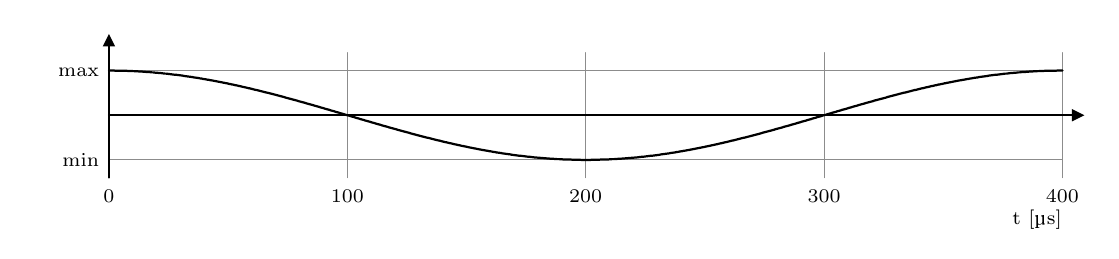
\begin{tikzpicture}[x=0.01985cm,y=-0.01985cm,line cap=round,line join=round]
\useasboundingbox (0,0) rectangle (680,130);
\path[draw=black!45,line width=0.35pt] (52,96) -- (52,16);
\path[draw=black!45,line width=0.35pt] (204.5,96) -- (204.5,16);
\path[draw=black!45,line width=0.35pt] (357,96) -- (357,16);
\path[draw=black!45,line width=0.35pt] (509.5,96) -- (509.5,16);
\path[draw=black!45,line width=0.35pt] (662,96) -- (662,16);
\path[draw=black!45,line width=0.35pt] (52,27.4) -- (662,27.4);
\path[draw=black!45,line width=0.35pt] (52,84.6) -- (662,84.6);
\path[draw=black,line width=0.7pt] (52,56) -- (670,56);
\path[fill=black,draw=none] (676,56) -- (668,52) -- (668,60) -- cycle;
\path[draw=black,line width=0.7pt] (52,96) -- (52,10);
\path[fill=black,draw=none] (52,4) -- (48,12) -- (56,12) -- cycle;
\node[anchor=base,inner sep=0pt,font=\scriptsize] at (52,112) {0};
\node[anchor=base,inner sep=0pt,font=\scriptsize] at (204.5,112) {100};
\node[anchor=base,inner sep=0pt,font=\scriptsize] at (357,112) {200};
\node[anchor=base,inner sep=0pt,font=\scriptsize] at (509.5,112) {300};
\node[anchor=base,inner sep=0pt,font=\scriptsize] at (662,112) {400};
\node[anchor=base east,inner sep=0pt,font=\scriptsize] at (46,31.4) {max};
\node[anchor=base east,inner sep=0pt,font=\scriptsize] at (46,88.6) {min};
\node[anchor=base east,inner sep=0pt,font=\scriptsize] at (662,126) {t [\textmu{}s]};
\path[draw=black,line width=0.8pt] (52,27.4) -- (52.8,27.4) -- (53.5,27.4) -- (54.3,27.4) -- (55.1,27.4) -- (55.8,27.5) -- (56.6,27.5) -- (57.3,27.5) -- (58.1,27.5) -- (58.9,27.5) -- (59.6,27.5) -- (60.4,27.5) -- (61.2,27.6) -- (61.9,27.6) -- (62.7,27.6) -- (63.4,27.6) -- (64.2,27.7) -- (65,27.7) -- (65.7,27.7) -- (66.5,27.7) -- (67.3,27.8) -- (68,27.8) -- (68.8,27.9) -- (69.5,27.9) -- (70.3,27.9) -- (71.1,28) -- (71.8,28) -- (72.6,28.1) -- (73.4,28.1) -- (74.1,28.2) -- (74.9,28.2) -- (75.6,28.3) -- (76.4,28.3) -- (77.2,28.4) -- (77.9,28.4) -- (78.7,28.5) -- (79.5,28.6) -- (80.2,28.6) -- (81,28.7) -- (81.7,28.8) -- (82.5,28.8) -- (83.3,28.9) -- (84,29) -- (84.8,29) -- (85.6,29.1) -- (86.3,29.2) -- (87.1,29.3) -- (87.8,29.4) -- (88.6,29.4) -- (89.4,29.5) -- (90.1,29.6) -- (90.9,29.7) -- (91.7,29.8) -- (92.4,29.9) -- (93.2,30) -- (93.9,30.1) -- (94.7,30.1) -- (95.5,30.2) -- (96.2,30.3) -- (97,30.4) -- (97.8,30.5) -- (98.5,30.6) -- (99.3,30.7) -- (100,30.9) -- (100.8,31) -- (101.6,31.1) -- (102.3,31.2) -- (103.1,31.3) -- (103.9,31.4) -- (104.6,31.5) -- (105.4,31.6) -- (106.1,31.8) -- (106.9,31.9) -- (107.7,32) -- (108.4,32.1) -- (109.2,32.2) -- (110,32.4) -- (110.7,32.5) -- (111.5,32.6) -- (112.2,32.8) -- (113,32.9) -- (113.8,33) -- (114.5,33.2) -- (115.3,33.3) -- (116.1,33.4) -- (116.8,33.6) -- (117.6,33.7) -- (118.3,33.8) -- (119.1,34) -- (119.9,34.1) -- (120.6,34.3) -- (121.4,34.4) -- (122.2,34.6) -- (122.9,34.7) -- (123.7,34.9) -- (124.4,35) -- (125.2,35.2) -- (126,35.3) -- (126.7,35.5) -- (127.5,35.6) -- (128.3,35.8) -- (129,36) -- (129.8,36.1) -- (130.5,36.3) -- (131.3,36.4) -- (132.1,36.6) -- (132.8,36.8) -- (133.6,36.9) -- (134.4,37.1) -- (135.1,37.3) -- (135.9,37.4) -- (136.6,37.6) -- (137.4,37.8) -- (138.2,38) -- (138.9,38.1) -- (139.7,38.3) -- (140.5,38.5) -- (141.2,38.7) -- (142,38.8) -- (142.7,39) -- (143.5,39.2) -- (144.3,39.4) -- (145,39.6) -- (145.8,39.8) -- (146.6,39.9) -- (147.3,40.1) -- (148.1,40.3) -- (148.8,40.5) -- (149.6,40.7) -- (150.4,40.9) -- (151.1,41.1) -- (151.9,41.3) -- (152.7,41.5) -- (153.4,41.6) -- (154.2,41.8) -- (154.9,42) -- (155.7,42.2) -- (156.5,42.4) -- (157.2,42.6) -- (158,42.8) -- (158.8,43) -- (159.5,43.2) -- (160.3,43.4) -- (161,43.6) -- (161.8,43.8) -- (162.6,44) -- (163.3,44.2) -- (164.1,44.4) -- (164.9,44.7) -- (165.6,44.9) -- (166.4,45.1) -- (167.1,45.3) -- (167.9,45.5) -- (168.7,45.7) -- (169.4,45.9) -- (170.2,46.1) -- (171,46.3) -- (171.7,46.5) -- (172.5,46.7) -- (173.2,47) -- (174,47.2) -- (174.8,47.4) -- (175.5,47.6) -- (176.3,47.8) -- (177.1,48) -- (177.8,48.2) -- (178.6,48.5) -- (179.3,48.7) -- (180.1,48.9) -- (180.9,49.1) -- (181.6,49.3) -- (182.4,49.5) -- (183.2,49.8) -- (183.9,50) -- (184.7,50.2) -- (185.4,50.4) -- (186.2,50.6) -- (187,50.9) -- (187.7,51.1) -- (188.5,51.3) -- (189.3,51.5) -- (190,51.8) -- (190.8,52) -- (191.5,52.2) -- (192.3,52.4) -- (193.1,52.6) -- (193.8,52.9) -- (194.6,53.1) -- (195.4,53.3) -- (196.1,53.5) -- (196.9,53.8) -- (197.6,54) -- (198.4,54.2) -- (199.2,54.4) -- (199.9,54.7) -- (200.7,54.9) -- (201.5,55.1) -- (202.2,55.3) -- (203,55.6) -- (203.7,55.8) -- (204.5,56) -- (205.3,56.2) -- (206,56.4) -- (206.8,56.7) -- (207.6,56.9) -- (208.3,57.1) -- (209.1,57.3) -- (209.8,57.6) -- (210.6,57.8) -- (211.4,58) -- (212.1,58.2) -- (212.9,58.5) -- (213.7,58.7) -- (214.4,58.9) -- (215.2,59.1) -- (215.9,59.4) -- (216.7,59.6) -- (217.5,59.8) -- (218.2,60) -- (219,60.2) -- (219.8,60.5) -- (220.5,60.7) -- (221.3,60.9) -- (222,61.1) -- (222.8,61.4) -- (223.6,61.6) -- (224.3,61.8) -- (225.1,62) -- (225.9,62.2) -- (226.6,62.5) -- (227.4,62.7) -- (228.1,62.9) -- (228.9,63.1) -- (229.7,63.3) -- (230.4,63.5) -- (231.2,63.8) -- (232,64) -- (232.7,64.2) -- (233.5,64.4) -- (234.2,64.6) -- (235,64.8) -- (235.8,65) -- (236.5,65.3) -- (237.3,65.5) -- (238.1,65.7) -- (238.8,65.9) -- (239.6,66.1) -- (240.3,66.3) -- (241.1,66.5) -- (241.9,66.7) -- (242.6,66.9) -- (243.4,67.1) -- (244.2,67.3) -- (244.9,67.6) -- (245.7,67.8) -- (246.4,68) -- (247.2,68.2) -- (248,68.4) -- (248.7,68.6) -- (249.5,68.8) -- (250.3,69) -- (251,69.2) -- (251.8,69.4) -- (252.5,69.6) -- (253.3,69.8) -- (254.1,70) -- (254.8,70.2) -- (255.6,70.4) -- (256.4,70.5) -- (257.1,70.7) -- (257.9,70.9) -- (258.6,71.1) -- (259.4,71.3) -- (260.2,71.5) -- (260.9,71.7) -- (261.7,71.9) -- (262.5,72.1) -- (263.2,72.2) -- (264,72.4) -- (264.7,72.6) -- (265.5,72.8) -- (266.3,73) -- (267,73.2) -- (267.8,73.3) -- (268.5,73.5) -- (269.3,73.7) -- (270.1,73.9) -- (270.8,74) -- (271.6,74.2) -- (272.4,74.4) -- (273.1,74.6) -- (273.9,74.7) -- (274.7,74.9) -- (275.4,75.1) -- (276.2,75.2) -- (276.9,75.4) -- (277.7,75.6) -- (278.5,75.7) -- (279.2,75.9) -- (280,76) -- (280.8,76.2) -- (281.5,76.4) -- (282.3,76.5) -- (283,76.7) -- (283.8,76.8) -- (284.6,77) -- (285.3,77.1) -- (286.1,77.3) -- (286.9,77.4) -- (287.6,77.6) -- (288.4,77.7) -- (289.1,77.9) -- (289.9,78) -- (290.7,78.2) -- (291.4,78.3) -- (292.2,78.4) -- (293,78.6) -- (293.7,78.7) -- (294.5,78.8) -- (295.2,79) -- (296,79.1) -- (296.8,79.2) -- (297.5,79.4) -- (298.3,79.5) -- (299.1,79.6) -- (299.8,79.8) -- (300.6,79.9) -- (301.3,80) -- (302.1,80.1) -- (302.9,80.2) -- (303.6,80.4) -- (304.4,80.5) -- (305.2,80.6) -- (305.9,80.7) -- (306.7,80.8) -- (307.4,80.9) -- (308.2,81) -- (309,81.1) -- (309.7,81.3) -- (310.5,81.4) -- (311.3,81.5) -- (312,81.6) -- (312.8,81.7) -- (313.5,81.8) -- (314.3,81.9) -- (315.1,81.9) -- (315.8,82) -- (316.6,82.1) -- (317.4,82.2) -- (318.1,82.3) -- (318.9,82.4) -- (319.6,82.5) -- (320.4,82.6) -- (321.2,82.6) -- (321.9,82.7) -- (322.7,82.8) -- (323.5,82.9) -- (324.2,83) -- (325,83) -- (325.7,83.1) -- (326.5,83.2) -- (327.3,83.2) -- (328,83.3) -- (328.8,83.4) -- (329.6,83.4) -- (330.3,83.5) -- (331.1,83.6) -- (331.8,83.6) -- (332.6,83.7) -- (333.4,83.7) -- (334.1,83.8) -- (334.9,83.8) -- (335.7,83.9) -- (336.4,83.9) -- (337.2,84) -- (337.9,84) -- (338.7,84.1) -- (339.5,84.1) -- (340.2,84.1) -- (341,84.2) -- (341.8,84.2) -- (342.5,84.3) -- (343.3,84.3) -- (344,84.3) -- (344.8,84.3) -- (345.6,84.4) -- (346.3,84.4) -- (347.1,84.4) -- (347.8,84.4) -- (348.6,84.5) -- (349.4,84.5) -- (350.1,84.5) -- (350.9,84.5) -- (351.7,84.5) -- (352.4,84.5) -- (353.2,84.5) -- (354,84.6) -- (354.7,84.6) -- (355.5,84.6) -- (356.2,84.6) -- (357,84.6) -- (357.8,84.6) -- (358.5,84.6) -- (359.3,84.6) -- (360.1,84.6) -- (360.8,84.5) -- (361.6,84.5) -- (362.3,84.5) -- (363.1,84.5) -- (363.9,84.5) -- (364.6,84.5) -- (365.4,84.5) -- (366.2,84.4) -- (366.9,84.4) -- (367.7,84.4) -- (368.4,84.4) -- (369.2,84.3) -- (370,84.3) -- (370.7,84.3) -- (371.5,84.3) -- (372.3,84.2) -- (373,84.2) -- (373.8,84.1) -- (374.5,84.1) -- (375.3,84.1) -- (376.1,84) -- (376.8,84) -- (377.6,83.9) -- (378.4,83.9) -- (379.1,83.8) -- (379.9,83.8) -- (380.6,83.7) -- (381.4,83.7) -- (382.2,83.6) -- (382.9,83.6) -- (383.7,83.5) -- (384.5,83.4) -- (385.2,83.4) -- (386,83.3) -- (386.7,83.2) -- (387.5,83.2) -- (388.3,83.1) -- (389,83) -- (389.8,83) -- (390.6,82.9) -- (391.3,82.8) -- (392.1,82.7) -- (392.8,82.6) -- (393.6,82.6) -- (394.4,82.5) -- (395.1,82.4) -- (395.9,82.3) -- (396.7,82.2) -- (397.4,82.1) -- (398.2,82) -- (398.9,81.9) -- (399.7,81.9) -- (400.5,81.8) -- (401.2,81.7) -- (402,81.6) -- (402.8,81.5) -- (403.5,81.4) -- (404.3,81.3) -- (405,81.1) -- (405.8,81) -- (406.6,80.9) -- (407.3,80.8) -- (408.1,80.7) -- (408.8,80.6) -- (409.6,80.5) -- (410.4,80.4) -- (411.1,80.2) -- (411.9,80.1) -- (412.7,80) -- (413.4,79.9) -- (414.2,79.8) -- (415,79.6) -- (415.7,79.5) -- (416.5,79.4) -- (417.2,79.2) -- (418,79.1) -- (418.8,79) -- (419.5,78.8) -- (420.3,78.7) -- (421.1,78.6) -- (421.8,78.4) -- (422.6,78.3) -- (423.3,78.2) -- (424.1,78) -- (424.9,77.9) -- (425.6,77.7) -- (426.4,77.6) -- (427.2,77.4) -- (427.9,77.3) -- (428.7,77.1) -- (429.4,77) -- (430.2,76.8) -- (431,76.7) -- (431.7,76.5) -- (432.5,76.4) -- (433.3,76.2) -- (434,76) -- (434.8,75.9) -- (435.5,75.7) -- (436.3,75.6) -- (437.1,75.4) -- (437.8,75.2) -- (438.6,75.1) -- (439.4,74.9) -- (440.1,74.7) -- (440.9,74.6) -- (441.6,74.4) -- (442.4,74.2) -- (443.2,74) -- (443.9,73.9) -- (444.7,73.7) -- (445.5,73.5) -- (446.2,73.3) -- (447,73.2) -- (447.7,73) -- (448.5,72.8) -- (449.3,72.6) -- (450,72.4) -- (450.8,72.2) -- (451.6,72.1) -- (452.3,71.9) -- (453.1,71.7) -- (453.8,71.5) -- (454.6,71.3) -- (455.4,71.1) -- (456.1,70.9) -- (456.9,70.7) -- (457.7,70.5) -- (458.4,70.4) -- (459.2,70.2) -- (459.9,70) -- (460.7,69.8) -- (461.5,69.6) -- (462.2,69.4) -- (463,69.2) -- (463.8,69) -- (464.5,68.8) -- (465.3,68.6) -- (466,68.4) -- (466.8,68.2) -- (467.6,68) -- (468.3,67.8) -- (469.1,67.6) -- (469.9,67.3) -- (470.6,67.1) -- (471.4,66.9) -- (472.1,66.7) -- (472.9,66.5) -- (473.7,66.3) -- (474.4,66.1) -- (475.2,65.9) -- (476,65.7) -- (476.7,65.5) -- (477.5,65.3) -- (478.2,65) -- (479,64.8) -- (479.8,64.6) -- (480.5,64.4) -- (481.3,64.2) -- (482.1,64) -- (482.8,63.8) -- (483.6,63.5) -- (484.3,63.3) -- (485.1,63.1) -- (485.9,62.9) -- (486.6,62.7) -- (487.4,62.5) -- (488.2,62.2) -- (488.9,62) -- (489.7,61.8) -- (490.4,61.6) -- (491.2,61.4) -- (492,61.1) -- (492.7,60.9) -- (493.5,60.7) -- (494.3,60.5) -- (495,60.2) -- (495.8,60) -- (496.5,59.8) -- (497.3,59.6) -- (498.1,59.4) -- (498.8,59.1) -- (499.6,58.9) -- (500.4,58.7) -- (501.1,58.5) -- (501.9,58.2) -- (502.6,58) -- (503.4,57.8) -- (504.2,57.6) -- (504.9,57.3) -- (505.7,57.1) -- (506.5,56.9) -- (507.2,56.7) -- (508,56.4) -- (508.7,56.2) -- (509.5,56) -- (510.3,55.8) -- (511,55.6) -- (511.8,55.3) -- (512.6,55.1) -- (513.3,54.9) -- (514.1,54.7) -- (514.8,54.4) -- (515.6,54.2) -- (516.4,54) -- (517.1,53.8) -- (517.9,53.5) -- (518.7,53.3) -- (519.4,53.1) -- (520.2,52.9) -- (520.9,52.6) -- (521.7,52.4) -- (522.5,52.2) -- (523.2,52) -- (524,51.8) -- (524.8,51.5) -- (525.5,51.3) -- (526.3,51.1) -- (527,50.9) -- (527.8,50.6) -- (528.6,50.4) -- (529.3,50.2) -- (530.1,50) -- (530.9,49.8) -- (531.6,49.5) -- (532.4,49.3) -- (533.1,49.1) -- (533.9,48.9) -- (534.7,48.7) -- (535.4,48.5) -- (536.2,48.2) -- (537,48) -- (537.7,47.8) -- (538.5,47.6) -- (539.2,47.4) -- (540,47.2) -- (540.8,47) -- (541.5,46.7) -- (542.3,46.5) -- (543.1,46.3) -- (543.8,46.1) -- (544.6,45.9) -- (545.3,45.7) -- (546.1,45.5) -- (546.9,45.3) -- (547.6,45.1) -- (548.4,44.9) -- (549.2,44.7) -- (549.9,44.4) -- (550.7,44.2) -- (551.4,44) -- (552.2,43.8) -- (553,43.6) -- (553.7,43.4) -- (554.5,43.2) -- (555.3,43) -- (556,42.8) -- (556.8,42.6) -- (557.5,42.4) -- (558.3,42.2) -- (559.1,42) -- (559.8,41.8) -- (560.6,41.6) -- (561.3,41.5) -- (562.1,41.3) -- (562.9,41.1) -- (563.6,40.9) -- (564.4,40.7) -- (565.2,40.5) -- (565.9,40.3) -- (566.7,40.1) -- (567.4,39.9) -- (568.2,39.8) -- (569,39.6) -- (569.7,39.4) -- (570.5,39.2) -- (571.3,39) -- (572,38.8) -- (572.8,38.7) -- (573.6,38.5) -- (574.3,38.3) -- (575.1,38.1) -- (575.8,38) -- (576.6,37.8) -- (577.4,37.6) -- (578.1,37.4) -- (578.9,37.3) -- (579.7,37.1) -- (580.4,36.9) -- (581.2,36.8) -- (581.9,36.6) -- (582.7,36.4) -- (583.5,36.3) -- (584.2,36.1) -- (585,36) -- (585.8,35.8) -- (586.5,35.6) -- (587.3,35.5) -- (588,35.3) -- (588.8,35.2) -- (589.6,35) -- (590.3,34.9) -- (591.1,34.7) -- (591.9,34.6) -- (592.6,34.4) -- (593.4,34.3) -- (594.1,34.1) -- (594.9,34) -- (595.7,33.8) -- (596.4,33.7) -- (597.2,33.6) -- (598,33.4) -- (598.7,33.3) -- (599.5,33.2) -- (600.2,33) -- (601,32.9) -- (601.8,32.8) -- (602.5,32.6) -- (603.3,32.5) -- (604.1,32.4) -- (604.8,32.2) -- (605.6,32.1) -- (606.3,32) -- (607.1,31.9) -- (607.9,31.8) -- (608.6,31.6) -- (609.4,31.5) -- (610.2,31.4) -- (610.9,31.3) -- (611.7,31.2) -- (612.4,31.1) -- (613.2,31) -- (614,30.9) -- (614.7,30.7) -- (615.5,30.6) -- (616.3,30.5) -- (617,30.4) -- (617.8,30.3) -- (618.5,30.2) -- (619.3,30.1) -- (620.1,30.1) -- (620.8,30) -- (621.6,29.9) -- (622.4,29.8) -- (623.1,29.7) -- (623.9,29.6) -- (624.6,29.5) -- (625.4,29.4) -- (626.2,29.4) -- (626.9,29.3) -- (627.7,29.2) -- (628.4,29.1) -- (629.2,29) -- (630,29) -- (630.7,28.9) -- (631.5,28.8) -- (632.3,28.8) -- (633,28.7) -- (633.8,28.6) -- (634.6,28.6) -- (635.3,28.5) -- (636.1,28.4) -- (636.8,28.4) -- (637.6,28.3) -- (638.4,28.3) -- (639.1,28.2) -- (639.9,28.2) -- (640.7,28.1) -- (641.4,28.1) -- (642.2,28) -- (642.9,28) -- (643.7,27.9) -- (644.5,27.9) -- (645.2,27.9) -- (646,27.8) -- (646.8,27.8) -- (647.5,27.7) -- (648.3,27.7) -- (649,27.7) -- (649.8,27.7) -- (650.6,27.6) -- (651.3,27.6) -- (652.1,27.6) -- (652.9,27.6) -- (653.6,27.5) -- (654.4,27.5) -- (655.1,27.5) -- (655.9,27.5) -- (656.7,27.5) -- (657.4,27.5) -- (658.2,27.5) -- (659,27.4) -- (659.7,27.4) -- (660.5,27.4) -- (661.2,27.4) -- (662,27.4);
\end{tikzpicture}\end{center}

\textbf{Az FM-jel (alsó csatorna), f\_D = 25 kHz}\par
\begin{center}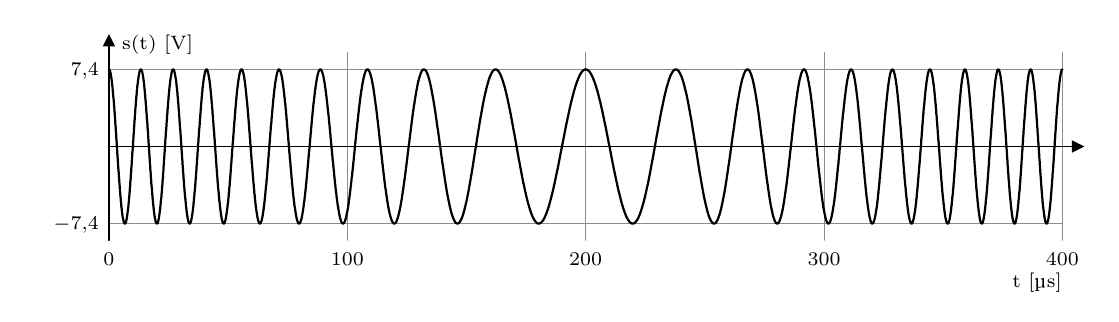
\begin{tikzpicture}[x=0.01985cm,y=-0.01985cm,line cap=round,line join=round]
\useasboundingbox (0,0) rectangle (680,170);
\path[draw=black!45,line width=0.35pt] (52,136) -- (52,16);
\path[draw=black!45,line width=0.35pt] (204.5,136) -- (204.5,16);
\path[draw=black!45,line width=0.35pt] (357,136) -- (357,16);
\path[draw=black!45,line width=0.35pt] (509.5,136) -- (509.5,16);
\path[draw=black!45,line width=0.35pt] (662,136) -- (662,16);
\path[draw=black!45,line width=0.35pt] (52,26.7) -- (662,26.7);
\path[draw=black!45,line width=0.35pt] (52,125.3) -- (662,125.3);
\path[draw=black,line width=0.7pt] (52,76) -- (670,76);
\path[fill=black,draw=none] (676,76) -- (668,72) -- (668,80) -- cycle;
\path[draw=black,line width=0.7pt] (52,136) -- (52,10);
\path[fill=black,draw=none] (52,4) -- (48,12) -- (56,12) -- cycle;
\node[anchor=base,inner sep=0pt,font=\scriptsize] at (52,152) {0};
\node[anchor=base,inner sep=0pt,font=\scriptsize] at (204.5,152) {100};
\node[anchor=base,inner sep=0pt,font=\scriptsize] at (357,152) {200};
\node[anchor=base,inner sep=0pt,font=\scriptsize] at (509.5,152) {300};
\node[anchor=base,inner sep=0pt,font=\scriptsize] at (662,152) {400};
\node[anchor=base east,inner sep=0pt,font=\scriptsize] at (46,30.7) {7,4};
\node[anchor=base east,inner sep=0pt,font=\scriptsize] at (46,129.3) {$-$7,4};
\node[anchor=base east,inner sep=0pt,font=\scriptsize] at (662,166) {t [\textmu{}s]};
\node[anchor=base west,inner sep=0pt,font=\scriptsize] at (60,14) {s(t) [V]};
\path[draw=black,line width=0.8pt] (52,26.7) -- (52.2,26.7) -- (52.3,26.9) -- (52.5,27.2) -- (52.6,27.5) -- (52.8,28) -- (52.9,28.6) -- (53.1,29.3) -- (53.2,30.1) -- (53.4,31) -- (53.5,32) -- (53.7,33.1) -- (53.8,34.3) -- (54,35.6) -- (54.1,37) -- (54.3,38.5) -- (54.4,40) -- (54.6,41.7) -- (54.7,43.4) -- (54.9,45.2) -- (55.1,47) -- (55.2,48.9) -- (55.4,50.9) -- (55.5,52.9) -- (55.7,55) -- (55.8,57.1) -- (56,59.3) -- (56.1,61.5) -- (56.3,63.7) -- (56.4,66) -- (56.6,68.3) -- (56.7,70.6) -- (56.9,72.9) -- (57,75.2) -- (57.2,77.5) -- (57.3,79.9) -- (57.5,82.2) -- (57.6,84.5) -- (57.8,86.7) -- (57.9,89) -- (58.1,91.2) -- (58.3,93.4) -- (58.4,95.6) -- (58.6,97.7) -- (58.7,99.7) -- (58.9,101.8) -- (59,103.7) -- (59.2,105.6) -- (59.3,107.4) -- (59.5,109.2) -- (59.6,110.9) -- (59.8,112.5) -- (59.9,114) -- (60.1,115.4) -- (60.2,116.8) -- (60.4,118) -- (60.5,119.2) -- (60.7,120.3) -- (60.8,121.3) -- (61,122.1) -- (61.2,122.9) -- (61.3,123.6) -- (61.5,124.1) -- (61.6,124.6) -- (61.8,124.9) -- (61.9,125.2) -- (62.1,125.3) -- (62.2,125.3) -- (62.4,125.2) -- (62.5,125) -- (62.7,124.7) -- (62.8,124.3) -- (63,123.8) -- (63.1,123.2) -- (63.3,122.5) -- (63.4,121.6) -- (63.6,120.7) -- (63.7,119.7) -- (63.9,118.5) -- (64,117.3) -- (64.2,116) -- (64.4,114.6) -- (64.5,113.1) -- (64.7,111.6) -- (64.8,109.9) -- (65,108.2) -- (65.1,106.4) -- (65.3,104.5) -- (65.4,102.6) -- (65.6,100.6) -- (65.7,98.6) -- (65.9,96.5) -- (66,94.4) -- (66.2,92.2) -- (66.3,90) -- (66.5,87.8) -- (66.6,85.5) -- (66.8,83.2) -- (66.9,80.9) -- (67.1,78.6) -- (67.3,76.3) -- (67.4,74) -- (67.6,71.7) -- (67.7,69.4) -- (67.9,67.1) -- (68,64.8) -- (68.2,62.6) -- (68.3,60.4) -- (68.5,58.2) -- (68.6,56.1) -- (68.8,54) -- (68.9,51.9) -- (69.1,49.9) -- (69.2,48) -- (69.4,46.1) -- (69.5,44.3) -- (69.7,42.6) -- (69.8,40.9) -- (70,39.3) -- (70.1,37.8) -- (70.3,36.4) -- (70.5,35.1) -- (70.6,33.8) -- (70.8,32.7) -- (70.9,31.6) -- (71.1,30.7) -- (71.2,29.8) -- (71.4,29) -- (71.5,28.4) -- (71.7,27.8) -- (71.8,27.4) -- (72,27) -- (72.1,26.8) -- (72.3,26.7) -- (72.4,26.7) -- (72.6,26.8) -- (72.7,27) -- (72.9,27.3) -- (73,27.7) -- (73.2,28.2) -- (73.4,28.8) -- (73.5,29.5) -- (73.7,30.4) -- (73.8,31.3) -- (74,32.3) -- (74.1,33.4) -- (74.3,34.6) -- (74.4,36) -- (74.6,37.3) -- (74.7,38.8) -- (74.9,40.4) -- (75,42) -- (75.2,43.7) -- (75.3,45.5) -- (75.5,47.3) -- (75.6,49.2) -- (75.8,51.2) -- (75.9,53.2) -- (76.1,55.3) -- (76.2,57.4) -- (76.4,59.5) -- (76.6,61.7) -- (76.7,63.9) -- (76.9,66.2) -- (77,68.4) -- (77.2,70.7) -- (77.3,73) -- (77.5,75.3) -- (77.6,77.6) -- (77.8,79.9) -- (77.9,82.2) -- (78.1,84.4) -- (78.2,86.7) -- (78.4,88.9) -- (78.5,91.1) -- (78.7,93.3) -- (78.8,95.4) -- (79,97.5) -- (79.1,99.6) -- (79.3,101.5) -- (79.5,103.5) -- (79.6,105.4) -- (79.8,107.2) -- (79.9,108.9) -- (80.1,110.6) -- (80.2,112.2) -- (80.4,113.7) -- (80.5,115.1) -- (80.7,116.5) -- (80.8,117.8) -- (81,118.9) -- (81.1,120) -- (81.3,121) -- (81.4,121.9) -- (81.6,122.7) -- (81.7,123.4) -- (81.9,124) -- (82,124.4) -- (82.2,124.8) -- (82.3,125.1) -- (82.5,125.3) -- (82.7,125.3) -- (82.8,125.3) -- (83,125.1) -- (83.1,124.9) -- (83.3,124.5) -- (83.4,124.1) -- (83.6,123.5) -- (83.7,122.8) -- (83.9,122.1) -- (84,121.2) -- (84.2,120.2) -- (84.3,119.2) -- (84.5,118) -- (84.6,116.8) -- (84.8,115.5) -- (84.9,114.1) -- (85.1,112.6) -- (85.2,111) -- (85.4,109.4) -- (85.6,107.7) -- (85.7,105.9) -- (85.9,104) -- (86,102.1) -- (86.2,100.2) -- (86.3,98.2) -- (86.5,96.1) -- (86.6,94) -- (86.8,91.9) -- (86.9,89.7) -- (87.1,87.5) -- (87.2,85.3) -- (87.4,83) -- (87.5,80.8) -- (87.7,78.5) -- (87.8,76.2) -- (88,74) -- (88.1,71.7) -- (88.3,69.4) -- (88.4,67.2) -- (88.6,65) -- (88.8,62.8) -- (88.9,60.6) -- (89.1,58.5) -- (89.2,56.4) -- (89.4,54.3) -- (89.5,52.3) -- (89.7,50.3) -- (89.8,48.4) -- (90,46.6) -- (90.1,44.8) -- (90.3,43.1) -- (90.4,41.4) -- (90.6,39.8) -- (90.7,38.3) -- (90.9,36.9) -- (91,35.6) -- (91.2,34.3) -- (91.3,33.1) -- (91.5,32.1) -- (91.7,31.1) -- (91.8,30.2) -- (92,29.4) -- (92.1,28.7) -- (92.3,28.1) -- (92.4,27.6) -- (92.6,27.2) -- (92.7,26.9) -- (92.9,26.8) -- (93,26.7) -- (93.2,26.7) -- (93.3,26.8) -- (93.5,27) -- (93.6,27.4) -- (93.8,27.8) -- (93.9,28.3) -- (94.1,28.9) -- (94.2,29.7) -- (94.4,30.5) -- (94.5,31.4) -- (94.7,32.4) -- (94.9,33.5) -- (95,34.7) -- (95.2,36) -- (95.3,37.3) -- (95.5,38.8) -- (95.6,40.3) -- (95.8,41.9) -- (95.9,43.5) -- (96.1,45.3) -- (96.2,47) -- (96.4,48.9) -- (96.5,50.8) -- (96.7,52.8) -- (96.8,54.8) -- (97,56.8) -- (97.1,58.9) -- (97.3,61) -- (97.4,63.2) -- (97.6,65.3) -- (97.8,67.5) -- (97.9,69.7) -- (98.1,72) -- (98.2,74.2) -- (98.4,76.4) -- (98.5,78.7) -- (98.7,80.9) -- (98.8,83.1) -- (99,85.3) -- (99.1,87.5) -- (99.3,89.7) -- (99.4,91.8) -- (99.6,93.9) -- (99.7,96) -- (99.9,98) -- (100,100) -- (100.2,101.9) -- (100.3,103.8) -- (100.5,105.6) -- (100.6,107.3) -- (100.8,109) -- (101,110.6) -- (101.1,112.2) -- (101.3,113.7) -- (101.4,115.1) -- (101.6,116.4) -- (101.7,117.6) -- (101.9,118.8) -- (102,119.8) -- (102.2,120.8) -- (102.3,121.7) -- (102.5,122.5) -- (102.6,123.2) -- (102.8,123.8) -- (102.9,124.3) -- (103.1,124.7) -- (103.2,125) -- (103.4,125.2) -- (103.5,125.3) -- (103.7,125.3) -- (103.9,125.2) -- (104,125) -- (104.2,124.8) -- (104.3,124.4) -- (104.5,123.9) -- (104.6,123.3) -- (104.8,122.6) -- (104.9,121.8) -- (105.1,121) -- (105.2,120) -- (105.4,119) -- (105.5,117.9) -- (105.7,116.7) -- (105.8,115.4) -- (106,114) -- (106.1,112.5) -- (106.3,111) -- (106.4,109.4) -- (106.6,107.8) -- (106.7,106.1) -- (106.9,104.3) -- (107.1,102.5) -- (107.2,100.6) -- (107.4,98.6) -- (107.5,96.7) -- (107.7,94.6) -- (107.8,92.6) -- (108,90.5) -- (108.1,88.4) -- (108.3,86.2) -- (108.4,84.1) -- (108.6,81.9) -- (108.7,79.7) -- (108.9,77.5) -- (109,75.3) -- (109.2,73.1) -- (109.3,71) -- (109.5,68.8) -- (109.6,66.6) -- (109.8,64.5) -- (110,62.4) -- (110.1,60.3) -- (110.3,58.2) -- (110.4,56.2) -- (110.6,54.2) -- (110.7,52.3) -- (110.9,50.4) -- (111,48.5) -- (111.2,46.7) -- (111.3,45) -- (111.5,43.3) -- (111.6,41.7) -- (111.8,40.2) -- (111.9,38.7) -- (112.1,37.3) -- (112.2,36) -- (112.4,34.8) -- (112.5,33.6) -- (112.7,32.6) -- (112.8,31.6) -- (113,30.7) -- (113.2,29.9) -- (113.3,29.1) -- (113.5,28.5) -- (113.6,28) -- (113.8,27.5) -- (113.9,27.2) -- (114.1,26.9) -- (114.2,26.7) -- (114.4,26.7) -- (114.5,26.7) -- (114.7,26.8) -- (114.8,27) -- (115,27.4) -- (115.1,27.8) -- (115.3,28.3) -- (115.4,28.9) -- (115.6,29.5) -- (115.7,30.3) -- (115.9,31.2) -- (116.1,32.1) -- (116.2,33.1) -- (116.4,34.3) -- (116.5,35.4) -- (116.7,36.7) -- (116.8,38.1) -- (117,39.5) -- (117.1,40.9) -- (117.3,42.5) -- (117.4,44.1) -- (117.6,45.8) -- (117.7,47.5) -- (117.9,49.3) -- (118,51.1) -- (118.2,53) -- (118.3,54.9) -- (118.5,56.9) -- (118.6,58.9) -- (118.8,60.9) -- (118.9,63) -- (119.1,65.1) -- (119.3,67.2) -- (119.4,69.3) -- (119.6,71.4) -- (119.7,73.6) -- (119.9,75.7) -- (120,77.9) -- (120.2,80) -- (120.3,82.1) -- (120.5,84.2) -- (120.6,86.3) -- (120.8,88.4) -- (120.9,90.5) -- (121.1,92.5) -- (121.2,94.5) -- (121.4,96.5) -- (121.5,98.4) -- (121.7,100.3) -- (121.8,102.1) -- (122,103.9) -- (122.2,105.6) -- (122.3,107.3) -- (122.5,108.9) -- (122.6,110.5) -- (122.8,112) -- (122.9,113.4) -- (123.1,114.7) -- (123.2,116) -- (123.4,117.2) -- (123.5,118.3) -- (123.7,119.4) -- (123.8,120.4) -- (124,121.3) -- (124.1,122.1) -- (124.3,122.8) -- (124.4,123.4) -- (124.6,123.9) -- (124.7,124.4) -- (124.9,124.8) -- (125,125) -- (125.2,125.2) -- (125.4,125.3) -- (125.5,125.3) -- (125.7,125.2) -- (125.8,125.1) -- (126,124.8) -- (126.1,124.4) -- (126.3,124) -- (126.4,123.5) -- (126.6,122.8) -- (126.7,122.1) -- (126.9,121.4) -- (127,120.5) -- (127.2,119.5) -- (127.3,118.5) -- (127.5,117.4) -- (127.6,116.2) -- (127.8,115) -- (127.9,113.6) -- (128.1,112.3) -- (128.3,110.8) -- (128.4,109.3) -- (128.6,107.7) -- (128.7,106.1) -- (128.9,104.4) -- (129,102.6) -- (129.2,100.9) -- (129.3,99) -- (129.5,97.2) -- (129.6,95.3) -- (129.8,93.3) -- (129.9,91.3) -- (130.1,89.3) -- (130.2,87.3) -- (130.4,85.3) -- (130.5,83.2) -- (130.7,81.2) -- (130.8,79.1) -- (131,77) -- (131.1,74.9) -- (131.3,72.8) -- (131.5,70.8) -- (131.6,68.7) -- (131.8,66.7) -- (131.9,64.6) -- (132.1,62.6) -- (132.2,60.6) -- (132.4,58.7) -- (132.5,56.8) -- (132.7,54.9) -- (132.8,53) -- (133,51.2) -- (133.1,49.4) -- (133.3,47.7) -- (133.4,46) -- (133.6,44.4) -- (133.7,42.9) -- (133.9,41.4) -- (134,39.9) -- (134.2,38.6) -- (134.4,37.2) -- (134.5,36) -- (134.7,34.8) -- (134.8,33.7) -- (135,32.7) -- (135.1,31.8) -- (135.3,30.9) -- (135.4,30.1) -- (135.6,29.4) -- (135.7,28.7) -- (135.9,28.2) -- (136,27.7) -- (136.2,27.4) -- (136.3,27.1) -- (136.5,26.8) -- (136.6,26.7) -- (136.8,26.7) -- (136.9,26.7) -- (137.1,26.8) -- (137.2,27) -- (137.4,27.3) -- (137.6,27.7) -- (137.7,28.2) -- (137.9,28.7) -- (138,29.3) -- (138.2,30) -- (138.3,30.8) -- (138.5,31.7) -- (138.6,32.6) -- (138.8,33.6) -- (138.9,34.7) -- (139.1,35.8) -- (139.2,37.1) -- (139.4,38.3) -- (139.5,39.7) -- (139.7,41.1) -- (139.8,42.6) -- (140,44.1) -- (140.1,45.6) -- (140.3,47.3) -- (140.5,48.9) -- (140.6,50.6) -- (140.8,52.4) -- (140.9,54.2) -- (141.1,56) -- (141.2,57.9) -- (141.4,59.8) -- (141.5,61.7) -- (141.7,63.7) -- (141.8,65.6) -- (142,67.6) -- (142.1,69.6) -- (142.3,71.6) -- (142.4,73.6) -- (142.6,75.6) -- (142.7,77.6) -- (142.9,79.6) -- (143,81.6) -- (143.2,83.6) -- (143.3,85.6) -- (143.5,87.5) -- (143.7,89.5) -- (143.8,91.4) -- (144,93.3) -- (144.1,95.1) -- (144.3,97) -- (144.4,98.8) -- (144.6,100.5) -- (144.7,102.2) -- (144.9,103.9) -- (145,105.5) -- (145.2,107.1) -- (145.3,108.6) -- (145.5,110.1) -- (145.6,111.5) -- (145.8,112.9) -- (145.9,114.1) -- (146.1,115.4) -- (146.2,116.5) -- (146.4,117.6) -- (146.6,118.7) -- (146.7,119.6) -- (146.9,120.5) -- (147,121.3) -- (147.2,122.1) -- (147.3,122.8) -- (147.5,123.3) -- (147.6,123.9) -- (147.8,124.3) -- (147.9,124.7) -- (148.1,125) -- (148.2,125.2) -- (148.4,125.3) -- (148.5,125.3) -- (148.7,125.3) -- (148.8,125.2) -- (149,125) -- (149.1,124.7) -- (149.3,124.4) -- (149.4,124) -- (149.6,123.5) -- (149.8,122.9) -- (149.9,122.3) -- (150.1,121.5) -- (150.2,120.8) -- (150.4,119.9) -- (150.5,119) -- (150.7,118) -- (150.8,116.9) -- (151,115.8) -- (151.1,114.6) -- (151.3,113.3) -- (151.4,112) -- (151.6,110.7) -- (151.7,109.3) -- (151.9,107.8) -- (152,106.3) -- (152.2,104.7) -- (152.3,103.1) -- (152.5,101.5) -- (152.7,99.8) -- (152.8,98.1) -- (153,96.3) -- (153.1,94.5) -- (153.3,92.7) -- (153.4,90.9) -- (153.6,89) -- (153.7,87.1) -- (153.9,85.2) -- (154,83.3) -- (154.2,81.4) -- (154.3,79.5) -- (154.5,77.6) -- (154.6,75.6) -- (154.8,73.7) -- (154.9,71.8) -- (155.1,69.9) -- (155.2,68) -- (155.4,66.1) -- (155.5,64.2) -- (155.7,62.3) -- (155.9,60.5) -- (156,58.7) -- (156.2,56.9) -- (156.3,55.1) -- (156.5,53.4) -- (156.6,51.7) -- (156.8,50.1) -- (156.9,48.5) -- (157.1,46.9) -- (157.2,45.4) -- (157.4,43.9) -- (157.5,42.5) -- (157.7,41.1) -- (157.8,39.8) -- (158,38.5) -- (158.1,37.3) -- (158.3,36.2) -- (158.4,35.1) -- (158.6,34) -- (158.8,33.1) -- (158.9,32.2) -- (159.1,31.3) -- (159.2,30.5) -- (159.4,29.8) -- (159.5,29.2) -- (159.7,28.6) -- (159.8,28.1) -- (160,27.7) -- (160.1,27.4) -- (160.3,27.1) -- (160.4,26.9) -- (160.6,26.7) -- (160.7,26.7) -- (160.9,26.7) -- (161,26.8) -- (161.2,26.9) -- (161.3,27.1) -- (161.5,27.4) -- (161.6,27.8) -- (161.8,28.2) -- (162,28.7) -- (162.1,29.3) -- (162.3,29.9) -- (162.4,30.6) -- (162.6,31.4) -- (162.7,32.2) -- (162.9,33.1) -- (163,34.1) -- (163.2,35.1) -- (163.3,36.2) -- (163.5,37.3) -- (163.6,38.5) -- (163.8,39.7) -- (163.9,41) -- (164.1,42.4) -- (164.2,43.8) -- (164.4,45.2) -- (164.5,46.7) -- (164.7,48.2) -- (164.9,49.7) -- (165,51.3) -- (165.2,53) -- (165.3,54.6) -- (165.5,56.3) -- (165.6,58) -- (165.8,59.7) -- (165.9,61.5) -- (166.1,63.3) -- (166.2,65.1) -- (166.4,66.9) -- (166.5,68.7) -- (166.7,70.5) -- (166.8,72.4) -- (167,74.2) -- (167.1,76) -- (167.3,77.9) -- (167.4,79.7) -- (167.6,81.5) -- (167.7,83.4) -- (167.9,85.2) -- (168.1,87) -- (168.2,88.8) -- (168.4,90.5) -- (168.5,92.3) -- (168.7,94) -- (168.8,95.7) -- (169,97.3) -- (169.1,99) -- (169.3,100.6) -- (169.4,102.1) -- (169.6,103.6) -- (169.7,105.1) -- (169.9,106.6) -- (170,108) -- (170.2,109.4) -- (170.3,110.7) -- (170.5,111.9) -- (170.6,113.2) -- (170.8,114.3) -- (171,115.4) -- (171.1,116.5) -- (171.3,117.5) -- (171.4,118.5) -- (171.6,119.4) -- (171.7,120.2) -- (171.9,121) -- (172,121.7) -- (172.2,122.3) -- (172.3,122.9) -- (172.5,123.4) -- (172.6,123.9) -- (172.8,124.3) -- (172.9,124.6) -- (173.1,124.9) -- (173.2,125.1) -- (173.4,125.2) -- (173.5,125.3) -- (173.7,125.3) -- (173.8,125.3) -- (174,125.2) -- (174.2,125) -- (174.3,124.7) -- (174.5,124.4) -- (174.6,124) -- (174.8,123.6) -- (174.9,123.1) -- (175.1,122.5) -- (175.2,121.9) -- (175.4,121.2) -- (175.5,120.5) -- (175.7,119.7) -- (175.8,118.8) -- (176,117.9) -- (176.1,117) -- (176.3,115.9) -- (176.4,114.9) -- (176.6,113.8) -- (176.7,112.6) -- (176.9,111.4) -- (177.1,110.1) -- (177.2,108.8) -- (177.4,107.5) -- (177.5,106.1) -- (177.7,104.7) -- (177.8,103.3) -- (178,101.8) -- (178.1,100.3) -- (178.3,98.7) -- (178.4,97.2) -- (178.6,95.6) -- (178.7,93.9) -- (178.9,92.3) -- (179,90.6) -- (179.2,88.9) -- (179.3,87.2) -- (179.5,85.5) -- (179.6,83.8) -- (179.8,82.1) -- (179.9,80.4) -- (180.1,78.6) -- (180.3,76.9) -- (180.4,75.1) -- (180.6,73.4) -- (180.7,71.7) -- (180.9,69.9) -- (181,68.2) -- (181.2,66.5) -- (181.3,64.8) -- (181.5,63.1) -- (181.6,61.5) -- (181.8,59.8) -- (181.9,58.2) -- (182.1,56.6) -- (182.2,55) -- (182.4,53.5) -- (182.5,52) -- (182.7,50.5) -- (182.8,49) -- (183,47.6) -- (183.2,46.2) -- (183.3,44.9) -- (183.5,43.5) -- (183.6,42.3) -- (183.8,41) -- (183.9,39.8) -- (184.1,38.7) -- (184.2,37.6) -- (184.4,36.6) -- (184.5,35.6) -- (184.7,34.6) -- (184.8,33.7) -- (185,32.8) -- (185.1,32) -- (185.3,31.3) -- (185.4,30.6) -- (185.6,30) -- (185.7,29.4) -- (185.9,28.9) -- (186,28.4) -- (186.2,28) -- (186.4,27.6) -- (186.5,27.3) -- (186.7,27.1) -- (186.8,26.9) -- (187,26.8) -- (187.1,26.7) -- (187.3,26.7) -- (187.4,26.7) -- (187.6,26.8) -- (187.7,27) -- (187.9,27.2) -- (188,27.5) -- (188.2,27.8) -- (188.3,28.2) -- (188.5,28.6) -- (188.6,29.1) -- (188.8,29.7) -- (188.9,30.3) -- (189.1,30.9) -- (189.3,31.6) -- (189.4,32.4) -- (189.6,33.2) -- (189.7,34) -- (189.9,34.9) -- (190,35.9) -- (190.2,36.9) -- (190.3,37.9) -- (190.5,39) -- (190.6,40.1) -- (190.8,41.3) -- (190.9,42.5) -- (191.1,43.7) -- (191.2,45) -- (191.4,46.3) -- (191.5,47.6) -- (191.7,49) -- (191.8,50.4) -- (192,51.8) -- (192.1,53.2) -- (192.3,54.7) -- (192.5,56.2) -- (192.6,57.7) -- (192.8,59.3) -- (192.9,60.8) -- (193.1,62.4) -- (193.2,64) -- (193.4,65.6) -- (193.5,67.2) -- (193.7,68.8) -- (193.8,70.4) -- (194,72) -- (194.1,73.7) -- (194.3,75.3) -- (194.4,76.9) -- (194.6,78.6) -- (194.7,80.2) -- (194.9,81.8) -- (195,83.4) -- (195.2,85) -- (195.4,86.6) -- (195.5,88.2) -- (195.7,89.7) -- (195.8,91.3) -- (196,92.8) -- (196.1,94.3) -- (196.3,95.8) -- (196.4,97.3) -- (196.6,98.7) -- (196.7,100.2) -- (196.9,101.5) -- (197,102.9) -- (197.2,104.2) -- (197.3,105.5) -- (197.5,106.8) -- (197.6,108.1) -- (197.8,109.3) -- (197.9,110.4) -- (198.1,111.6) -- (198.2,112.6) -- (198.4,113.7) -- (198.6,114.7) -- (198.7,115.7) -- (198.9,116.6) -- (199,117.5) -- (199.2,118.3) -- (199.3,119.1) -- (199.5,119.9) -- (199.6,120.6) -- (199.8,121.2) -- (199.9,121.8) -- (200.1,122.4) -- (200.2,122.9) -- (200.4,123.4) -- (200.5,123.8) -- (200.7,124.2) -- (200.8,124.5) -- (201,124.8) -- (201.1,125) -- (201.3,125.1) -- (201.5,125.3) -- (201.6,125.3) -- (201.8,125.3) -- (201.9,125.3) -- (202.1,125.2) -- (202.2,125.1) -- (202.4,124.9) -- (202.5,124.7) -- (202.7,124.4) -- (202.8,124.1) -- (203,123.7) -- (203.1,123.3) -- (203.3,122.8) -- (203.4,122.3) -- (203.6,121.7) -- (203.7,121.1) -- (203.9,120.4) -- (204,119.7) -- (204.2,119) -- (204.3,118.2) -- (204.5,117.4) -- (204.7,116.5) -- (204.8,115.6) -- (205,114.7) -- (205.1,113.7) -- (205.3,112.7) -- (205.4,111.6) -- (205.6,110.6) -- (205.7,109.4) -- (205.9,108.3) -- (206,107.1) -- (206.2,105.9) -- (206.3,104.7) -- (206.5,103.4) -- (206.6,102.1) -- (206.8,100.8) -- (206.9,99.5) -- (207.1,98.1) -- (207.2,96.7) -- (207.4,95.4) -- (207.6,93.9) -- (207.7,92.5) -- (207.9,91.1) -- (208,89.6) -- (208.2,88.1) -- (208.3,86.7) -- (208.5,85.2) -- (208.6,83.7) -- (208.8,82.2) -- (208.9,80.7) -- (209.1,79.2) -- (209.2,77.7) -- (209.4,76.1) -- (209.5,74.6) -- (209.7,73.1) -- (209.8,71.6) -- (210,70.1) -- (210.1,68.6) -- (210.3,67.1) -- (210.4,65.7) -- (210.6,64.2) -- (210.8,62.8) -- (210.9,61.3) -- (211.1,59.9) -- (211.2,58.5) -- (211.4,57.1) -- (211.5,55.7) -- (211.7,54.4) -- (211.8,53) -- (212,51.7) -- (212.1,50.5) -- (212.3,49.2) -- (212.4,48) -- (212.6,46.7) -- (212.7,45.6) -- (212.9,44.4) -- (213,43.3) -- (213.2,42.2) -- (213.3,41.1) -- (213.5,40.1) -- (213.7,39.1) -- (213.8,38.1) -- (214,37.2) -- (214.1,36.3) -- (214.3,35.5) -- (214.4,34.6) -- (214.6,33.9) -- (214.7,33.1) -- (214.9,32.4) -- (215,31.7) -- (215.2,31.1) -- (215.3,30.5) -- (215.5,30) -- (215.6,29.5) -- (215.8,29) -- (215.9,28.6) -- (216.1,28.2) -- (216.2,27.9) -- (216.4,27.6) -- (216.5,27.3) -- (216.7,27.1) -- (216.9,26.9) -- (217,26.8) -- (217.2,26.7) -- (217.3,26.7) -- (217.5,26.7) -- (217.6,26.7) -- (217.8,26.8) -- (217.9,26.9) -- (218.1,27.1) -- (218.2,27.3) -- (218.4,27.6) -- (218.5,27.9) -- (218.7,28.2) -- (218.8,28.6) -- (219,29) -- (219.1,29.4) -- (219.3,29.9) -- (219.4,30.4) -- (219.6,31) -- (219.8,31.6) -- (219.9,32.3) -- (220.1,32.9) -- (220.2,33.7) -- (220.4,34.4) -- (220.5,35.2) -- (220.7,36) -- (220.8,36.9) -- (221,37.7) -- (221.1,38.6) -- (221.3,39.6) -- (221.4,40.6) -- (221.6,41.6) -- (221.7,42.6) -- (221.9,43.6) -- (222,44.7) -- (222.2,45.8) -- (222.3,46.9) -- (222.5,48.1) -- (222.6,49.3) -- (222.8,50.5) -- (223,51.7) -- (223.1,52.9) -- (223.3,54.1) -- (223.4,55.4) -- (223.6,56.7) -- (223.7,58) -- (223.9,59.3) -- (224,60.6) -- (224.2,61.9) -- (224.3,63.3) -- (224.5,64.6) -- (224.6,66) -- (224.8,67.3) -- (224.9,68.7) -- (225.1,70.1) -- (225.2,71.5) -- (225.4,72.9) -- (225.5,74.2) -- (225.7,75.6) -- (225.9,77) -- (226,78.4) -- (226.2,79.8) -- (226.3,81.1) -- (226.5,82.5) -- (226.6,83.9) -- (226.8,85.2) -- (226.9,86.6) -- (227.1,87.9) -- (227.2,89.2) -- (227.4,90.5) -- (227.5,91.8) -- (227.7,93.1) -- (227.8,94.4) -- (228,95.7) -- (228.1,96.9) -- (228.3,98.1) -- (228.4,99.3) -- (228.6,100.5) -- (228.7,101.7) -- (228.9,102.8) -- (229.1,104) -- (229.2,105.1) -- (229.4,106.2) -- (229.5,107.2) -- (229.7,108.2) -- (229.8,109.3) -- (230,110.2) -- (230.1,111.2) -- (230.3,112.1) -- (230.4,113) -- (230.6,113.9) -- (230.7,114.8) -- (230.9,115.6) -- (231,116.4) -- (231.2,117.1) -- (231.3,117.8) -- (231.5,118.5) -- (231.6,119.2) -- (231.8,119.8) -- (232,120.4) -- (232.1,121) -- (232.3,121.5) -- (232.4,122) -- (232.6,122.5) -- (232.7,122.9) -- (232.9,123.3) -- (233,123.7) -- (233.2,124) -- (233.3,124.3) -- (233.5,124.5) -- (233.6,124.7) -- (233.8,124.9) -- (233.9,125.1) -- (234.1,125.2) -- (234.2,125.3) -- (234.4,125.3) -- (234.5,125.3) -- (234.7,125.3) -- (234.8,125.2) -- (235,125.2) -- (235.2,125) -- (235.3,124.9) -- (235.5,124.7) -- (235.6,124.4) -- (235.8,124.2) -- (235.9,123.9) -- (236.1,123.5) -- (236.2,123.2) -- (236.4,122.8) -- (236.5,122.3) -- (236.7,121.9) -- (236.8,121.4) -- (237,120.9) -- (237.1,120.3) -- (237.3,119.7) -- (237.4,119.1) -- (237.6,118.5) -- (237.7,117.8) -- (237.9,117.1) -- (238.1,116.4) -- (238.2,115.6) -- (238.4,114.8) -- (238.5,114) -- (238.7,113.2) -- (238.8,112.3) -- (239,111.5) -- (239.1,110.6) -- (239.3,109.6) -- (239.4,108.7) -- (239.6,107.7) -- (239.7,106.7) -- (239.9,105.7) -- (240,104.7) -- (240.2,103.7) -- (240.3,102.6) -- (240.5,101.5) -- (240.6,100.4) -- (240.8,99.3) -- (240.9,98.2) -- (241.1,97.1) -- (241.3,95.9) -- (241.4,94.8) -- (241.6,93.6) -- (241.7,92.4) -- (241.9,91.2) -- (242,90) -- (242.2,88.8) -- (242.3,87.6) -- (242.5,86.4) -- (242.6,85.1) -- (242.8,83.9) -- (242.9,82.7) -- (243.1,81.4) -- (243.2,80.2) -- (243.4,78.9) -- (243.5,77.7) -- (243.7,76.4) -- (243.8,75.2) -- (244,73.9) -- (244.2,72.7) -- (244.3,71.5) -- (244.5,70.2) -- (244.6,69) -- (244.8,67.8) -- (244.9,66.6) -- (245.1,65.4) -- (245.2,64.1) -- (245.4,63) -- (245.5,61.8) -- (245.7,60.6) -- (245.8,59.4) -- (246,58.3) -- (246.1,57.1) -- (246.3,56) -- (246.4,54.9) -- (246.6,53.8) -- (246.7,52.7) -- (246.9,51.6) -- (247,50.6) -- (247.2,49.5) -- (247.4,48.5) -- (247.5,47.5) -- (247.7,46.5) -- (247.8,45.6) -- (248,44.6) -- (248.1,43.7) -- (248.3,42.8) -- (248.4,41.9) -- (248.6,41) -- (248.7,40.2) -- (248.9,39.4) -- (249,38.6) -- (249.2,37.8) -- (249.3,37.1) -- (249.5,36.3) -- (249.6,35.6) -- (249.8,34.9) -- (249.9,34.3) -- (250.1,33.7) -- (250.3,33.1) -- (250.4,32.5) -- (250.6,31.9) -- (250.7,31.4) -- (250.9,30.9) -- (251,30.4) -- (251.2,30) -- (251.3,29.6) -- (251.5,29.2) -- (251.6,28.8) -- (251.8,28.5) -- (251.9,28.2) -- (252.1,27.9) -- (252.2,27.7) -- (252.4,27.4) -- (252.5,27.2) -- (252.7,27.1) -- (252.8,26.9) -- (253,26.8) -- (253.1,26.7) -- (253.3,26.7) -- (253.5,26.7) -- (253.6,26.7) -- (253.8,26.7) -- (253.9,26.8) -- (254.1,26.8) -- (254.2,27) -- (254.4,27.1) -- (254.5,27.3) -- (254.7,27.5) -- (254.8,27.7) -- (255,27.9) -- (255.1,28.2) -- (255.3,28.5) -- (255.4,28.8) -- (255.6,29.2) -- (255.7,29.6) -- (255.9,30) -- (256,30.4) -- (256.2,30.9) -- (256.4,31.4) -- (256.5,31.9) -- (256.7,32.4) -- (256.8,32.9) -- (257,33.5) -- (257.1,34.1) -- (257.3,34.7) -- (257.4,35.4) -- (257.6,36) -- (257.7,36.7) -- (257.9,37.4) -- (258,38.1) -- (258.2,38.9) -- (258.3,39.6) -- (258.5,40.4) -- (258.6,41.2) -- (258.8,42) -- (258.9,42.9) -- (259.1,43.7) -- (259.2,44.6) -- (259.4,45.5) -- (259.6,46.4) -- (259.7,47.3) -- (259.9,48.2) -- (260,49.1) -- (260.2,50.1) -- (260.3,51.1) -- (260.5,52.1) -- (260.6,53) -- (260.8,54) -- (260.9,55.1) -- (261.1,56.1) -- (261.2,57.1) -- (261.4,58.2) -- (261.5,59.2) -- (261.7,60.3) -- (261.8,61.3) -- (262,62.4) -- (262.1,63.5) -- (262.3,64.6) -- (262.5,65.6) -- (262.6,66.7) -- (262.8,67.8) -- (262.9,68.9) -- (263.1,70) -- (263.2,71.1) -- (263.4,72.2) -- (263.5,73.3) -- (263.7,74.4) -- (263.8,75.6) -- (264,76.7) -- (264.1,77.8) -- (264.3,78.9) -- (264.4,80) -- (264.6,81.1) -- (264.7,82.2) -- (264.9,83.2) -- (265,84.3) -- (265.2,85.4) -- (265.3,86.5) -- (265.5,87.5) -- (265.7,88.6) -- (265.8,89.7) -- (266,90.7) -- (266.1,91.7) -- (266.3,92.8) -- (266.4,93.8) -- (266.6,94.8) -- (266.7,95.8) -- (266.9,96.8) -- (267,97.8) -- (267.2,98.7) -- (267.3,99.7) -- (267.5,100.6) -- (267.6,101.6) -- (267.8,102.5) -- (267.9,103.4) -- (268.1,104.3) -- (268.2,105.2) -- (268.4,106) -- (268.5,106.9) -- (268.7,107.7) -- (268.9,108.5) -- (269,109.3) -- (269.2,110.1) -- (269.3,110.9) -- (269.5,111.6) -- (269.6,112.3) -- (269.8,113) -- (269.9,113.7) -- (270.1,114.4) -- (270.2,115.1) -- (270.4,115.7) -- (270.5,116.3) -- (270.7,116.9) -- (270.8,117.5) -- (271,118.1) -- (271.1,118.6) -- (271.3,119.2) -- (271.4,119.7) -- (271.6,120.1) -- (271.8,120.6) -- (271.9,121) -- (272.1,121.5) -- (272.2,121.9) -- (272.4,122.2) -- (272.5,122.6) -- (272.7,122.9) -- (272.8,123.2) -- (273,123.5) -- (273.1,123.8) -- (273.3,124) -- (273.4,124.3) -- (273.6,124.5) -- (273.7,124.7) -- (273.9,124.8) -- (274,125) -- (274.2,125.1) -- (274.3,125.2) -- (274.5,125.2) -- (274.7,125.3) -- (274.8,125.3) -- (275,125.3) -- (275.1,125.3) -- (275.3,125.3) -- (275.4,125.2) -- (275.6,125.1) -- (275.7,125) -- (275.9,124.9) -- (276,124.8) -- (276.2,124.6) -- (276.3,124.4) -- (276.5,124.2) -- (276.6,124) -- (276.8,123.8) -- (276.9,123.5) -- (277.1,123.2) -- (277.2,122.9) -- (277.4,122.6) -- (277.5,122.2) -- (277.7,121.8) -- (277.9,121.5) -- (278,121.1) -- (278.2,120.6) -- (278.3,120.2) -- (278.5,119.7) -- (278.6,119.3) -- (278.8,118.8) -- (278.9,118.2) -- (279.1,117.7) -- (279.2,117.2) -- (279.4,116.6) -- (279.5,116) -- (279.7,115.4) -- (279.8,114.8) -- (280,114.2) -- (280.1,113.5) -- (280.3,112.9) -- (280.4,112.2) -- (280.6,111.5) -- (280.8,110.8) -- (280.9,110.1) -- (281.1,109.3) -- (281.2,108.6) -- (281.4,107.8) -- (281.5,107.1) -- (281.7,106.3) -- (281.8,105.5) -- (282,104.7) -- (282.1,103.9) -- (282.3,103.1) -- (282.4,102.2) -- (282.6,101.4) -- (282.7,100.5) -- (282.9,99.7) -- (283,98.8) -- (283.2,97.9) -- (283.3,97) -- (283.5,96.1) -- (283.6,95.2) -- (283.8,94.3) -- (284,93.4) -- (284.1,92.5) -- (284.3,91.5) -- (284.4,90.6) -- (284.6,89.7) -- (284.7,88.7) -- (284.9,87.8) -- (285,86.8) -- (285.2,85.9) -- (285.3,84.9) -- (285.5,83.9) -- (285.6,83) -- (285.8,82) -- (285.9,81) -- (286.1,80.1) -- (286.2,79.1) -- (286.4,78.1) -- (286.5,77.2) -- (286.7,76.2) -- (286.9,75.2) -- (287,74.3) -- (287.2,73.3) -- (287.3,72.3) -- (287.5,71.4) -- (287.6,70.4) -- (287.8,69.4) -- (287.9,68.5) -- (288.1,67.5) -- (288.2,66.6) -- (288.4,65.7) -- (288.5,64.7) -- (288.7,63.8) -- (288.8,62.9) -- (289,61.9) -- (289.1,61) -- (289.3,60.1) -- (289.4,59.2) -- (289.6,58.3) -- (289.7,57.4) -- (289.9,56.6) -- (290.1,55.7) -- (290.2,54.8) -- (290.4,54) -- (290.5,53.1) -- (290.7,52.3) -- (290.8,51.5) -- (291,50.6) -- (291.1,49.8) -- (291.3,49) -- (291.4,48.2) -- (291.6,47.5) -- (291.7,46.7) -- (291.9,45.9) -- (292,45.2) -- (292.2,44.5) -- (292.3,43.8) -- (292.5,43.1) -- (292.6,42.4) -- (292.8,41.7) -- (293,41) -- (293.1,40.4) -- (293.3,39.7) -- (293.4,39.1) -- (293.6,38.5) -- (293.7,37.9) -- (293.9,37.3) -- (294,36.7) -- (294.2,36.2) -- (294.3,35.6) -- (294.5,35.1) -- (294.6,34.6) -- (294.8,34.1) -- (294.9,33.6) -- (295.1,33.1) -- (295.2,32.7) -- (295.4,32.2) -- (295.5,31.8) -- (295.7,31.4) -- (295.8,31) -- (296,30.7) -- (296.2,30.3) -- (296.3,30) -- (296.5,29.6) -- (296.6,29.3) -- (296.8,29) -- (296.9,28.8) -- (297.1,28.5) -- (297.2,28.3) -- (297.4,28.1) -- (297.5,27.8) -- (297.7,27.7) -- (297.8,27.5) -- (298,27.3) -- (298.1,27.2) -- (298.3,27.1) -- (298.4,27) -- (298.6,26.9) -- (298.7,26.8) -- (298.9,26.7) -- (299.1,26.7) -- (299.2,26.7) -- (299.4,26.7) -- (299.5,26.7) -- (299.7,26.7) -- (299.8,26.7) -- (300,26.8) -- (300.1,26.9) -- (300.3,27) -- (300.4,27.1) -- (300.6,27.2) -- (300.7,27.4) -- (300.9,27.5) -- (301,27.7) -- (301.2,27.9) -- (301.3,28.1) -- (301.5,28.3) -- (301.6,28.5) -- (301.8,28.8) -- (301.9,29.1) -- (302.1,29.4) -- (302.3,29.7) -- (302.4,30) -- (302.6,30.3) -- (302.7,30.6) -- (302.9,31) -- (303,31.4) -- (303.2,31.8) -- (303.3,32.2) -- (303.5,32.6) -- (303.6,33) -- (303.8,33.5) -- (303.9,33.9) -- (304.1,34.4) -- (304.2,34.9) -- (304.4,35.4) -- (304.5,35.9) -- (304.7,36.4) -- (304.8,36.9) -- (305,37.5) -- (305.2,38) -- (305.3,38.6) -- (305.5,39.2) -- (305.6,39.8) -- (305.8,40.4) -- (305.9,41) -- (306.1,41.6) -- (306.2,42.2) -- (306.4,42.9) -- (306.5,43.5) -- (306.7,44.2) -- (306.8,44.9) -- (307,45.6) -- (307.1,46.3) -- (307.3,47) -- (307.4,47.7) -- (307.6,48.4) -- (307.7,49.1) -- (307.9,49.9) -- (308,50.6) -- (308.2,51.4) -- (308.4,52.1) -- (308.5,52.9) -- (308.7,53.6) -- (308.8,54.4) -- (309,55.2) -- (309.1,56) -- (309.3,56.8) -- (309.4,57.6) -- (309.6,58.4) -- (309.7,59.2) -- (309.9,60) -- (310,60.8) -- (310.2,61.7) -- (310.3,62.5) -- (310.5,63.3) -- (310.6,64.2) -- (310.8,65) -- (310.9,65.8) -- (311.1,66.7) -- (311.3,67.5) -- (311.4,68.4) -- (311.6,69.2) -- (311.7,70.1) -- (311.9,70.9) -- (312,71.8) -- (312.2,72.6) -- (312.3,73.5) -- (312.5,74.3) -- (312.6,75.2) -- (312.8,76.1) -- (312.9,76.9) -- (313.1,77.8) -- (313.2,78.6) -- (313.4,79.5) -- (313.5,80.3) -- (313.7,81.2) -- (313.8,82) -- (314,82.8) -- (314.1,83.7) -- (314.3,84.5) -- (314.5,85.4) -- (314.6,86.2) -- (314.8,87) -- (314.9,87.8) -- (315.1,88.7) -- (315.2,89.5) -- (315.4,90.3) -- (315.5,91.1) -- (315.7,91.9) -- (315.8,92.7) -- (316,93.5) -- (316.1,94.3) -- (316.3,95.1) -- (316.4,95.8) -- (316.6,96.6) -- (316.7,97.4) -- (316.9,98.1) -- (317,98.9) -- (317.2,99.6) -- (317.4,100.3) -- (317.5,101.1) -- (317.7,101.8) -- (317.8,102.5) -- (318,103.2) -- (318.1,103.9) -- (318.3,104.6) -- (318.4,105.2) -- (318.6,105.9) -- (318.7,106.6) -- (318.9,107.2) -- (319,107.9) -- (319.2,108.5) -- (319.3,109.1) -- (319.5,109.7) -- (319.6,110.3) -- (319.8,110.9) -- (319.9,111.5) -- (320.1,112.1) -- (320.2,112.6) -- (320.4,113.2) -- (320.6,113.7) -- (320.7,114.3) -- (320.9,114.8) -- (321,115.3) -- (321.2,115.8) -- (321.3,116.3) -- (321.5,116.7) -- (321.6,117.2) -- (321.8,117.6) -- (321.9,118.1) -- (322.1,118.5) -- (322.2,118.9) -- (322.4,119.3) -- (322.5,119.7) -- (322.7,120.1) -- (322.8,120.4) -- (323,120.8) -- (323.1,121.1) -- (323.3,121.5) -- (323.5,121.8) -- (323.6,122.1) -- (323.8,122.4) -- (323.9,122.6) -- (324.1,122.9) -- (324.2,123.1) -- (324.4,123.4) -- (324.5,123.6) -- (324.7,123.8) -- (324.8,124) -- (325,124.2) -- (325.1,124.3) -- (325.3,124.5) -- (325.4,124.6) -- (325.6,124.8) -- (325.7,124.9) -- (325.9,125) -- (326,125.1) -- (326.2,125.2) -- (326.3,125.2) -- (326.5,125.3) -- (326.7,125.3) -- (326.8,125.3) -- (327,125.3) -- (327.1,125.3) -- (327.3,125.3) -- (327.4,125.3) -- (327.6,125.2) -- (327.7,125.2) -- (327.9,125.1) -- (328,125) -- (328.2,124.9) -- (328.3,124.8) -- (328.5,124.7) -- (328.6,124.5) -- (328.8,124.4) -- (328.9,124.2) -- (329.1,124.1) -- (329.2,123.9) -- (329.4,123.7) -- (329.6,123.5) -- (329.7,123.2) -- (329.9,123) -- (330,122.7) -- (330.2,122.5) -- (330.3,122.2) -- (330.5,121.9) -- (330.6,121.6) -- (330.8,121.3) -- (330.9,121) -- (331.1,120.6) -- (331.2,120.3) -- (331.4,119.9) -- (331.5,119.6) -- (331.7,119.2) -- (331.8,118.8) -- (332,118.4) -- (332.1,118) -- (332.3,117.5) -- (332.4,117.1) -- (332.6,116.7) -- (332.8,116.2) -- (332.9,115.7) -- (333.1,115.3) -- (333.2,114.8) -- (333.4,114.3) -- (333.5,113.8) -- (333.7,113.2) -- (333.8,112.7) -- (334,112.2) -- (334.1,111.6) -- (334.3,111.1) -- (334.4,110.5) -- (334.6,109.9) -- (334.7,109.4) -- (334.9,108.8) -- (335,108.2) -- (335.2,107.6) -- (335.3,107) -- (335.5,106.3) -- (335.7,105.7) -- (335.8,105.1) -- (336,104.4) -- (336.1,103.8) -- (336.3,103.1) -- (336.4,102.4) -- (336.6,101.8) -- (336.7,101.1) -- (336.9,100.4) -- (337,99.7) -- (337.2,99) -- (337.3,98.3) -- (337.5,97.6) -- (337.6,96.9) -- (337.8,96.2) -- (337.9,95.5) -- (338.1,94.7) -- (338.2,94) -- (338.4,93.3) -- (338.5,92.5) -- (338.7,91.8) -- (338.9,91) -- (339,90.3) -- (339.2,89.5) -- (339.3,88.7) -- (339.5,88) -- (339.6,87.2) -- (339.8,86.5) -- (339.9,85.7) -- (340.1,84.9) -- (340.2,84.1) -- (340.4,83.4) -- (340.5,82.6) -- (340.7,81.8) -- (340.8,81) -- (341,80.2) -- (341.1,79.5) -- (341.3,78.7) -- (341.4,77.9) -- (341.6,77.1) -- (341.8,76.3) -- (341.9,75.5) -- (342.1,74.7) -- (342.2,74) -- (342.4,73.2) -- (342.5,72.4) -- (342.7,71.6) -- (342.8,70.8) -- (343,70.1) -- (343.1,69.3) -- (343.3,68.5) -- (343.4,67.7) -- (343.6,67) -- (343.7,66.2) -- (343.9,65.4) -- (344,64.7) -- (344.2,63.9) -- (344.3,63.2) -- (344.5,62.4) -- (344.6,61.7) -- (344.8,60.9) -- (345,60.2) -- (345.1,59.4) -- (345.3,58.7) -- (345.4,58) -- (345.6,57.2) -- (345.7,56.5) -- (345.9,55.8) -- (346,55.1) -- (346.2,54.4) -- (346.3,53.7) -- (346.5,53) -- (346.6,52.3) -- (346.8,51.6) -- (346.9,51) -- (347.1,50.3) -- (347.2,49.6) -- (347.4,49) -- (347.5,48.3) -- (347.7,47.7) -- (347.8,47.1) -- (348,46.4) -- (348.2,45.8) -- (348.3,45.2) -- (348.5,44.6) -- (348.6,44) -- (348.8,43.4) -- (348.9,42.8) -- (349.1,42.3) -- (349.2,41.7) -- (349.4,41.1) -- (349.5,40.6) -- (349.7,40.1) -- (349.8,39.5) -- (350,39) -- (350.1,38.5) -- (350.3,38) -- (350.4,37.5) -- (350.6,37) -- (350.7,36.6) -- (350.9,36.1) -- (351.1,35.6) -- (351.2,35.2) -- (351.4,34.8) -- (351.5,34.4) -- (351.7,33.9) -- (351.8,33.5) -- (352,33.2) -- (352.1,32.8) -- (352.3,32.4) -- (352.4,32) -- (352.6,31.7) -- (352.7,31.4) -- (352.9,31) -- (353,30.7) -- (353.2,30.4) -- (353.3,30.1) -- (353.5,29.9) -- (353.6,29.6) -- (353.8,29.3) -- (354,29.1) -- (354.1,28.8) -- (354.3,28.6) -- (354.4,28.4) -- (354.6,28.2) -- (354.7,28) -- (354.9,27.9) -- (355,27.7) -- (355.2,27.5) -- (355.3,27.4) -- (355.5,27.3) -- (355.6,27.2) -- (355.8,27.1) -- (355.9,27) -- (356.1,26.9) -- (356.2,26.8) -- (356.4,26.8) -- (356.5,26.7) -- (356.7,26.7) -- (356.8,26.7) -- (357,26.7) -- (357.2,26.7) -- (357.3,26.7) -- (357.5,26.7) -- (357.6,26.8) -- (357.8,26.8) -- (357.9,26.9) -- (358.1,27) -- (358.2,27.1) -- (358.4,27.2) -- (358.5,27.3) -- (358.7,27.4) -- (358.8,27.5) -- (359,27.7) -- (359.1,27.9) -- (359.3,28) -- (359.4,28.2) -- (359.6,28.4) -- (359.7,28.6) -- (359.9,28.8) -- (360.1,29.1) -- (360.2,29.3) -- (360.4,29.6) -- (360.5,29.9) -- (360.7,30.1) -- (360.8,30.4) -- (361,30.7) -- (361.1,31) -- (361.3,31.4) -- (361.4,31.7) -- (361.6,32) -- (361.7,32.4) -- (361.9,32.8) -- (362,33.2) -- (362.2,33.5) -- (362.3,33.9) -- (362.5,34.4) -- (362.6,34.8) -- (362.8,35.2) -- (362.9,35.6) -- (363.1,36.1) -- (363.3,36.6) -- (363.4,37) -- (363.6,37.5) -- (363.7,38) -- (363.9,38.5) -- (364,39) -- (364.2,39.5) -- (364.3,40.1) -- (364.5,40.6) -- (364.6,41.1) -- (364.8,41.7) -- (364.9,42.3) -- (365.1,42.8) -- (365.2,43.4) -- (365.4,44) -- (365.5,44.6) -- (365.7,45.2) -- (365.8,45.8) -- (366,46.4) -- (366.2,47.1) -- (366.3,47.7) -- (366.5,48.3) -- (366.6,49) -- (366.8,49.6) -- (366.9,50.3) -- (367.1,51) -- (367.2,51.6) -- (367.4,52.3) -- (367.5,53) -- (367.7,53.7) -- (367.8,54.4) -- (368,55.1) -- (368.1,55.8) -- (368.3,56.5) -- (368.4,57.2) -- (368.6,58) -- (368.7,58.7) -- (368.9,59.4) -- (369,60.2) -- (369.2,60.9) -- (369.4,61.7) -- (369.5,62.4) -- (369.7,63.2) -- (369.8,63.9) -- (370,64.7) -- (370.1,65.4) -- (370.3,66.2) -- (370.4,67) -- (370.6,67.7) -- (370.7,68.5) -- (370.9,69.3) -- (371,70.1) -- (371.2,70.8) -- (371.3,71.6) -- (371.5,72.4) -- (371.6,73.2) -- (371.8,74) -- (371.9,74.7) -- (372.1,75.5) -- (372.3,76.3) -- (372.4,77.1) -- (372.6,77.9) -- (372.7,78.7) -- (372.9,79.5) -- (373,80.2) -- (373.2,81) -- (373.3,81.8) -- (373.5,82.6) -- (373.6,83.4) -- (373.8,84.1) -- (373.9,84.9) -- (374.1,85.7) -- (374.2,86.5) -- (374.4,87.2) -- (374.5,88) -- (374.7,88.7) -- (374.8,89.5) -- (375,90.3) -- (375.1,91) -- (375.3,91.8) -- (375.5,92.5) -- (375.6,93.3) -- (375.8,94) -- (375.9,94.7) -- (376.1,95.5) -- (376.2,96.2) -- (376.4,96.9) -- (376.5,97.6) -- (376.7,98.3) -- (376.8,99) -- (377,99.7) -- (377.1,100.4) -- (377.3,101.1) -- (377.4,101.8) -- (377.6,102.4) -- (377.7,103.1) -- (377.9,103.8) -- (378,104.4) -- (378.2,105.1) -- (378.4,105.7) -- (378.5,106.3) -- (378.7,107) -- (378.8,107.6) -- (379,108.2) -- (379.1,108.8) -- (379.3,109.4) -- (379.4,109.9) -- (379.6,110.5) -- (379.7,111.1) -- (379.9,111.6) -- (380,112.2) -- (380.2,112.7) -- (380.3,113.2) -- (380.5,113.8) -- (380.6,114.3) -- (380.8,114.8) -- (380.9,115.3) -- (381.1,115.7) -- (381.2,116.2) -- (381.4,116.7) -- (381.6,117.1) -- (381.7,117.5) -- (381.9,118) -- (382,118.4) -- (382.2,118.8) -- (382.3,119.2) -- (382.5,119.6) -- (382.6,119.9) -- (382.8,120.3) -- (382.9,120.6) -- (383.1,121) -- (383.2,121.3) -- (383.4,121.6) -- (383.5,121.9) -- (383.7,122.2) -- (383.8,122.5) -- (384,122.7) -- (384.1,123) -- (384.3,123.2) -- (384.5,123.5) -- (384.6,123.7) -- (384.8,123.9) -- (384.9,124.1) -- (385.1,124.2) -- (385.2,124.4) -- (385.4,124.5) -- (385.5,124.7) -- (385.7,124.8) -- (385.8,124.9) -- (386,125) -- (386.1,125.1) -- (386.3,125.2) -- (386.4,125.2) -- (386.6,125.3) -- (386.7,125.3) -- (386.9,125.3) -- (387,125.3) -- (387.2,125.3) -- (387.3,125.3) -- (387.5,125.3) -- (387.7,125.2) -- (387.8,125.2) -- (388,125.1) -- (388.1,125) -- (388.3,124.9) -- (388.4,124.8) -- (388.6,124.6) -- (388.7,124.5) -- (388.9,124.3) -- (389,124.2) -- (389.2,124) -- (389.3,123.8) -- (389.5,123.6) -- (389.6,123.4) -- (389.8,123.1) -- (389.9,122.9) -- (390.1,122.6) -- (390.2,122.4) -- (390.4,122.1) -- (390.6,121.8) -- (390.7,121.5) -- (390.9,121.1) -- (391,120.8) -- (391.2,120.4) -- (391.3,120.1) -- (391.5,119.7) -- (391.6,119.3) -- (391.8,118.9) -- (391.9,118.5) -- (392.1,118.1) -- (392.2,117.6) -- (392.4,117.2) -- (392.5,116.7) -- (392.7,116.3) -- (392.8,115.8) -- (393,115.3) -- (393.1,114.8) -- (393.3,114.3) -- (393.4,113.7) -- (393.6,113.2) -- (393.8,112.6) -- (393.9,112.1) -- (394.1,111.5) -- (394.2,110.9) -- (394.4,110.3) -- (394.5,109.7) -- (394.7,109.1) -- (394.8,108.5) -- (395,107.9) -- (395.1,107.2) -- (395.3,106.6) -- (395.4,105.9) -- (395.6,105.2) -- (395.7,104.6) -- (395.9,103.9) -- (396,103.2) -- (396.2,102.5) -- (396.3,101.8) -- (396.5,101.1) -- (396.7,100.3) -- (396.8,99.6) -- (397,98.9) -- (397.1,98.1) -- (397.3,97.4) -- (397.4,96.6) -- (397.6,95.8) -- (397.7,95.1) -- (397.9,94.3) -- (398,93.5) -- (398.2,92.7) -- (398.3,91.9) -- (398.5,91.1) -- (398.6,90.3) -- (398.8,89.5) -- (398.9,88.7) -- (399.1,87.8) -- (399.2,87) -- (399.4,86.2) -- (399.5,85.4) -- (399.7,84.5) -- (399.9,83.7) -- (400,82.8) -- (400.2,82) -- (400.3,81.2) -- (400.5,80.3) -- (400.6,79.5) -- (400.8,78.6) -- (400.9,77.8) -- (401.1,76.9) -- (401.2,76.1) -- (401.4,75.2) -- (401.5,74.3) -- (401.7,73.5) -- (401.8,72.6) -- (402,71.8) -- (402.1,70.9) -- (402.3,70.1) -- (402.4,69.2) -- (402.6,68.4) -- (402.8,67.5) -- (402.9,66.7) -- (403.1,65.8) -- (403.2,65) -- (403.4,64.2) -- (403.5,63.3) -- (403.7,62.5) -- (403.8,61.7) -- (404,60.8) -- (404.1,60) -- (404.3,59.2) -- (404.4,58.4) -- (404.6,57.6) -- (404.7,56.8) -- (404.9,56) -- (405,55.2) -- (405.2,54.4) -- (405.3,53.6) -- (405.5,52.9) -- (405.6,52.1) -- (405.8,51.4) -- (406,50.6) -- (406.1,49.9) -- (406.3,49.1) -- (406.4,48.4) -- (406.6,47.7) -- (406.7,47) -- (406.9,46.3) -- (407,45.6) -- (407.2,44.9) -- (407.3,44.2) -- (407.5,43.5) -- (407.6,42.9) -- (407.8,42.2) -- (407.9,41.6) -- (408.1,41) -- (408.2,40.4) -- (408.4,39.8) -- (408.5,39.2) -- (408.7,38.6) -- (408.8,38) -- (409,37.5) -- (409.2,36.9) -- (409.3,36.4) -- (409.5,35.9) -- (409.6,35.4) -- (409.8,34.9) -- (409.9,34.4) -- (410.1,33.9) -- (410.2,33.5) -- (410.4,33) -- (410.5,32.6) -- (410.7,32.2) -- (410.8,31.8) -- (411,31.4) -- (411.1,31) -- (411.3,30.6) -- (411.4,30.3) -- (411.6,30) -- (411.7,29.7) -- (411.9,29.4) -- (412.1,29.1) -- (412.2,28.8) -- (412.4,28.5) -- (412.5,28.3) -- (412.7,28.1) -- (412.8,27.9) -- (413,27.7) -- (413.1,27.5) -- (413.3,27.4) -- (413.4,27.2) -- (413.6,27.1) -- (413.7,27) -- (413.9,26.9) -- (414,26.8) -- (414.2,26.7) -- (414.3,26.7) -- (414.5,26.7) -- (414.6,26.7) -- (414.8,26.7) -- (415,26.7) -- (415.1,26.7) -- (415.3,26.8) -- (415.4,26.9) -- (415.6,27) -- (415.7,27.1) -- (415.9,27.2) -- (416,27.3) -- (416.2,27.5) -- (416.3,27.7) -- (416.5,27.8) -- (416.6,28.1) -- (416.8,28.3) -- (416.9,28.5) -- (417.1,28.8) -- (417.2,29) -- (417.4,29.3) -- (417.5,29.6) -- (417.7,30) -- (417.8,30.3) -- (418,30.7) -- (418.2,31) -- (418.3,31.4) -- (418.5,31.8) -- (418.6,32.2) -- (418.8,32.7) -- (418.9,33.1) -- (419.1,33.6) -- (419.2,34.1) -- (419.4,34.6) -- (419.5,35.1) -- (419.7,35.6) -- (419.8,36.2) -- (420,36.7) -- (420.1,37.3) -- (420.3,37.9) -- (420.4,38.5) -- (420.6,39.1) -- (420.7,39.7) -- (420.9,40.4) -- (421.1,41) -- (421.2,41.7) -- (421.4,42.4) -- (421.5,43.1) -- (421.7,43.8) -- (421.8,44.5) -- (422,45.2) -- (422.1,45.9) -- (422.3,46.7) -- (422.4,47.5) -- (422.6,48.2) -- (422.7,49) -- (422.9,49.8) -- (423,50.6) -- (423.2,51.5) -- (423.3,52.3) -- (423.5,53.1) -- (423.6,54) -- (423.8,54.8) -- (423.9,55.7) -- (424.1,56.6) -- (424.3,57.4) -- (424.4,58.3) -- (424.6,59.2) -- (424.7,60.1) -- (424.9,61) -- (425,61.9) -- (425.2,62.9) -- (425.3,63.8) -- (425.5,64.7) -- (425.6,65.7) -- (425.8,66.6) -- (425.9,67.5) -- (426.1,68.5) -- (426.2,69.4) -- (426.4,70.4) -- (426.5,71.4) -- (426.7,72.3) -- (426.8,73.3) -- (427,74.3) -- (427.2,75.2) -- (427.3,76.2) -- (427.5,77.2) -- (427.6,78.1) -- (427.8,79.1) -- (427.9,80.1) -- (428.1,81) -- (428.2,82) -- (428.4,83) -- (428.5,83.9) -- (428.7,84.9) -- (428.8,85.9) -- (429,86.8) -- (429.1,87.8) -- (429.3,88.7) -- (429.4,89.7) -- (429.6,90.6) -- (429.7,91.5) -- (429.9,92.5) -- (430,93.4) -- (430.2,94.3) -- (430.4,95.2) -- (430.5,96.1) -- (430.7,97) -- (430.8,97.9) -- (431,98.8) -- (431.1,99.7) -- (431.3,100.5) -- (431.4,101.4) -- (431.6,102.2) -- (431.7,103.1) -- (431.9,103.9) -- (432,104.7) -- (432.2,105.5) -- (432.3,106.3) -- (432.5,107.1) -- (432.6,107.8) -- (432.8,108.6) -- (432.9,109.3) -- (433.1,110.1) -- (433.3,110.8) -- (433.4,111.5) -- (433.6,112.2) -- (433.7,112.9) -- (433.9,113.5) -- (434,114.2) -- (434.2,114.8) -- (434.3,115.4) -- (434.5,116) -- (434.6,116.6) -- (434.8,117.2) -- (434.9,117.7) -- (435.1,118.2) -- (435.2,118.8) -- (435.4,119.3) -- (435.5,119.7) -- (435.7,120.2) -- (435.8,120.6) -- (436,121.1) -- (436.1,121.5) -- (436.3,121.8) -- (436.5,122.2) -- (436.6,122.6) -- (436.8,122.9) -- (436.9,123.2) -- (437.1,123.5) -- (437.2,123.8) -- (437.4,124) -- (437.5,124.2) -- (437.7,124.4) -- (437.8,124.6) -- (438,124.8) -- (438.1,124.9) -- (438.3,125) -- (438.4,125.1) -- (438.6,125.2) -- (438.7,125.3) -- (438.9,125.3) -- (439,125.3) -- (439.2,125.3) -- (439.4,125.3) -- (439.5,125.2) -- (439.7,125.2) -- (439.8,125.1) -- (440,125) -- (440.1,124.8) -- (440.3,124.7) -- (440.4,124.5) -- (440.6,124.3) -- (440.7,124) -- (440.9,123.8) -- (441,123.5) -- (441.2,123.2) -- (441.3,122.9) -- (441.5,122.6) -- (441.6,122.2) -- (441.8,121.9) -- (441.9,121.5) -- (442.1,121) -- (442.2,120.6) -- (442.4,120.1) -- (442.6,119.7) -- (442.7,119.2) -- (442.9,118.6) -- (443,118.1) -- (443.2,117.5) -- (443.3,116.9) -- (443.5,116.3) -- (443.6,115.7) -- (443.8,115.1) -- (443.9,114.4) -- (444.1,113.7) -- (444.2,113) -- (444.4,112.3) -- (444.5,111.6) -- (444.7,110.9) -- (444.8,110.1) -- (445,109.3) -- (445.1,108.5) -- (445.3,107.7) -- (445.5,106.9) -- (445.6,106) -- (445.8,105.2) -- (445.9,104.3) -- (446.1,103.4) -- (446.2,102.5) -- (446.4,101.6) -- (446.5,100.6) -- (446.7,99.7) -- (446.8,98.7) -- (447,97.8) -- (447.1,96.8) -- (447.3,95.8) -- (447.4,94.8) -- (447.6,93.8) -- (447.7,92.8) -- (447.9,91.7) -- (448,90.7) -- (448.2,89.7) -- (448.3,88.6) -- (448.5,87.5) -- (448.7,86.5) -- (448.8,85.4) -- (449,84.3) -- (449.1,83.2) -- (449.3,82.2) -- (449.4,81.1) -- (449.6,80) -- (449.7,78.9) -- (449.9,77.8) -- (450,76.7) -- (450.2,75.6) -- (450.3,74.4) -- (450.5,73.3) -- (450.6,72.2) -- (450.8,71.1) -- (450.9,70) -- (451.1,68.9) -- (451.2,67.8) -- (451.4,66.7) -- (451.6,65.6) -- (451.7,64.6) -- (451.9,63.5) -- (452,62.4) -- (452.2,61.3) -- (452.3,60.3) -- (452.5,59.2) -- (452.6,58.2) -- (452.8,57.1) -- (452.9,56.1) -- (453.1,55.1) -- (453.2,54) -- (453.4,53) -- (453.5,52.1) -- (453.7,51.1) -- (453.8,50.1) -- (454,49.1) -- (454.1,48.2) -- (454.3,47.3) -- (454.4,46.4) -- (454.6,45.5) -- (454.8,44.6) -- (454.9,43.7) -- (455.1,42.9) -- (455.2,42) -- (455.4,41.2) -- (455.5,40.4) -- (455.7,39.6) -- (455.8,38.9) -- (456,38.1) -- (456.1,37.4) -- (456.3,36.7) -- (456.4,36) -- (456.6,35.4) -- (456.7,34.7) -- (456.9,34.1) -- (457,33.5) -- (457.2,32.9) -- (457.3,32.4) -- (457.5,31.9) -- (457.7,31.4) -- (457.8,30.9) -- (458,30.4) -- (458.1,30) -- (458.3,29.6) -- (458.4,29.2) -- (458.6,28.8) -- (458.7,28.5) -- (458.9,28.2) -- (459,27.9) -- (459.2,27.7) -- (459.3,27.5) -- (459.5,27.3) -- (459.6,27.1) -- (459.8,27) -- (459.9,26.8) -- (460.1,26.8) -- (460.2,26.7) -- (460.4,26.7) -- (460.5,26.7) -- (460.7,26.7) -- (460.9,26.7) -- (461,26.8) -- (461.2,26.9) -- (461.3,27.1) -- (461.5,27.2) -- (461.6,27.4) -- (461.8,27.7) -- (461.9,27.9) -- (462.1,28.2) -- (462.2,28.5) -- (462.4,28.8) -- (462.5,29.2) -- (462.7,29.6) -- (462.8,30) -- (463,30.4) -- (463.1,30.9) -- (463.3,31.4) -- (463.4,31.9) -- (463.6,32.5) -- (463.8,33.1) -- (463.9,33.7) -- (464.1,34.3) -- (464.2,34.9) -- (464.4,35.6) -- (464.5,36.3) -- (464.7,37.1) -- (464.8,37.8) -- (465,38.6) -- (465.1,39.4) -- (465.3,40.2) -- (465.4,41) -- (465.6,41.9) -- (465.7,42.8) -- (465.9,43.7) -- (466,44.6) -- (466.2,45.6) -- (466.3,46.5) -- (466.5,47.5) -- (466.6,48.5) -- (466.8,49.5) -- (467,50.6) -- (467.1,51.6) -- (467.3,52.7) -- (467.4,53.8) -- (467.6,54.9) -- (467.7,56) -- (467.9,57.1) -- (468,58.3) -- (468.2,59.4) -- (468.3,60.6) -- (468.5,61.8) -- (468.6,63) -- (468.8,64.1) -- (468.9,65.4) -- (469.1,66.6) -- (469.2,67.8) -- (469.4,69) -- (469.5,70.2) -- (469.7,71.5) -- (469.9,72.7) -- (470,73.9) -- (470.2,75.2) -- (470.3,76.4) -- (470.5,77.7) -- (470.6,78.9) -- (470.8,80.2) -- (470.9,81.4) -- (471.1,82.7) -- (471.2,83.9) -- (471.4,85.1) -- (471.5,86.4) -- (471.7,87.6) -- (471.8,88.8) -- (472,90) -- (472.1,91.2) -- (472.3,92.4) -- (472.4,93.6) -- (472.6,94.8) -- (472.7,95.9) -- (472.9,97.1) -- (473.1,98.2) -- (473.2,99.3) -- (473.4,100.4) -- (473.5,101.5) -- (473.7,102.6) -- (473.8,103.7) -- (474,104.7) -- (474.1,105.7) -- (474.3,106.7) -- (474.4,107.7) -- (474.6,108.7) -- (474.7,109.6) -- (474.9,110.6) -- (475,111.5) -- (475.2,112.3) -- (475.3,113.2) -- (475.5,114) -- (475.6,114.8) -- (475.8,115.6) -- (476,116.4) -- (476.1,117.1) -- (476.3,117.8) -- (476.4,118.5) -- (476.6,119.1) -- (476.7,119.7) -- (476.9,120.3) -- (477,120.9) -- (477.2,121.4) -- (477.3,121.9) -- (477.5,122.3) -- (477.6,122.8) -- (477.8,123.2) -- (477.9,123.5) -- (478.1,123.9) -- (478.2,124.2) -- (478.4,124.4) -- (478.5,124.7) -- (478.7,124.9) -- (478.8,125) -- (479,125.2) -- (479.2,125.2) -- (479.3,125.3) -- (479.5,125.3) -- (479.6,125.3) -- (479.8,125.3) -- (479.9,125.2) -- (480.1,125.1) -- (480.2,124.9) -- (480.4,124.7) -- (480.5,124.5) -- (480.7,124.3) -- (480.8,124) -- (481,123.7) -- (481.1,123.3) -- (481.3,122.9) -- (481.4,122.5) -- (481.6,122) -- (481.7,121.5) -- (481.9,121) -- (482.1,120.4) -- (482.2,119.8) -- (482.4,119.2) -- (482.5,118.5) -- (482.7,117.8) -- (482.8,117.1) -- (483,116.4) -- (483.1,115.6) -- (483.3,114.8) -- (483.4,113.9) -- (483.6,113) -- (483.7,112.1) -- (483.9,111.2) -- (484,110.2) -- (484.2,109.3) -- (484.3,108.2) -- (484.5,107.2) -- (484.6,106.2) -- (484.8,105.1) -- (484.9,104) -- (485.1,102.8) -- (485.3,101.7) -- (485.4,100.5) -- (485.6,99.3) -- (485.7,98.1) -- (485.9,96.9) -- (486,95.7) -- (486.2,94.4) -- (486.3,93.1) -- (486.5,91.8) -- (486.6,90.5) -- (486.8,89.2) -- (486.9,87.9) -- (487.1,86.6) -- (487.2,85.2) -- (487.4,83.9) -- (487.5,82.5) -- (487.7,81.1) -- (487.8,79.8) -- (488,78.4) -- (488.2,77) -- (488.3,75.6) -- (488.5,74.2) -- (488.6,72.9) -- (488.8,71.5) -- (488.9,70.1) -- (489.1,68.7) -- (489.2,67.3) -- (489.4,66) -- (489.5,64.6) -- (489.7,63.3) -- (489.8,61.9) -- (490,60.6) -- (490.1,59.3) -- (490.3,58) -- (490.4,56.7) -- (490.6,55.4) -- (490.7,54.1) -- (490.9,52.9) -- (491,51.7) -- (491.2,50.5) -- (491.4,49.3) -- (491.5,48.1) -- (491.7,46.9) -- (491.8,45.8) -- (492,44.7) -- (492.1,43.6) -- (492.3,42.6) -- (492.4,41.6) -- (492.6,40.6) -- (492.7,39.6) -- (492.9,38.6) -- (493,37.7) -- (493.2,36.9) -- (493.3,36) -- (493.5,35.2) -- (493.6,34.4) -- (493.8,33.7) -- (493.9,32.9) -- (494.1,32.3) -- (494.3,31.6) -- (494.4,31) -- (494.6,30.4) -- (494.7,29.9) -- (494.9,29.4) -- (495,29) -- (495.2,28.6) -- (495.3,28.2) -- (495.5,27.9) -- (495.6,27.6) -- (495.8,27.3) -- (495.9,27.1) -- (496.1,26.9) -- (496.2,26.8) -- (496.4,26.7) -- (496.5,26.7) -- (496.7,26.7) -- (496.8,26.7) -- (497,26.8) -- (497.1,26.9) -- (497.3,27.1) -- (497.5,27.3) -- (497.6,27.6) -- (497.8,27.9) -- (497.9,28.2) -- (498.1,28.6) -- (498.2,29) -- (498.4,29.5) -- (498.5,30) -- (498.7,30.5) -- (498.8,31.1) -- (499,31.7) -- (499.1,32.4) -- (499.3,33.1) -- (499.4,33.9) -- (499.6,34.6) -- (499.7,35.5) -- (499.9,36.3) -- (500,37.2) -- (500.2,38.1) -- (500.4,39.1) -- (500.5,40.1) -- (500.7,41.1) -- (500.8,42.2) -- (501,43.3) -- (501.1,44.4) -- (501.3,45.6) -- (501.4,46.7) -- (501.6,48) -- (501.7,49.2) -- (501.9,50.5) -- (502,51.7) -- (502.2,53) -- (502.3,54.4) -- (502.5,55.7) -- (502.6,57.1) -- (502.8,58.5) -- (502.9,59.9) -- (503.1,61.3) -- (503.2,62.8) -- (503.4,64.2) -- (503.6,65.7) -- (503.7,67.1) -- (503.9,68.6) -- (504,70.1) -- (504.2,71.6) -- (504.3,73.1) -- (504.5,74.6) -- (504.6,76.1) -- (504.8,77.7) -- (504.9,79.2) -- (505.1,80.7) -- (505.2,82.2) -- (505.4,83.7) -- (505.5,85.2) -- (505.7,86.7) -- (505.8,88.1) -- (506,89.6) -- (506.1,91.1) -- (506.3,92.5) -- (506.5,93.9) -- (506.6,95.4) -- (506.8,96.7) -- (506.9,98.1) -- (507.1,99.5) -- (507.2,100.8) -- (507.4,102.1) -- (507.5,103.4) -- (507.7,104.7) -- (507.8,105.9) -- (508,107.1) -- (508.1,108.3) -- (508.3,109.4) -- (508.4,110.6) -- (508.6,111.6) -- (508.7,112.7) -- (508.9,113.7) -- (509,114.7) -- (509.2,115.6) -- (509.3,116.5) -- (509.5,117.4) -- (509.7,118.2) -- (509.8,119) -- (510,119.7) -- (510.1,120.4) -- (510.3,121.1) -- (510.4,121.7) -- (510.6,122.3) -- (510.7,122.8) -- (510.9,123.3) -- (511,123.7) -- (511.2,124.1) -- (511.3,124.4) -- (511.5,124.7) -- (511.6,124.9) -- (511.8,125.1) -- (511.9,125.2) -- (512.1,125.3) -- (512.2,125.3) -- (512.4,125.3) -- (512.6,125.3) -- (512.7,125.1) -- (512.9,125) -- (513,124.8) -- (513.2,124.5) -- (513.3,124.2) -- (513.5,123.8) -- (513.6,123.4) -- (513.8,122.9) -- (513.9,122.4) -- (514.1,121.8) -- (514.2,121.2) -- (514.4,120.6) -- (514.5,119.9) -- (514.7,119.1) -- (514.8,118.3) -- (515,117.5) -- (515.1,116.6) -- (515.3,115.7) -- (515.4,114.7) -- (515.6,113.7) -- (515.8,112.6) -- (515.9,111.6) -- (516.1,110.4) -- (516.2,109.3) -- (516.4,108.1) -- (516.5,106.8) -- (516.7,105.5) -- (516.8,104.2) -- (517,102.9) -- (517.1,101.5) -- (517.3,100.2) -- (517.4,98.7) -- (517.6,97.3) -- (517.7,95.8) -- (517.9,94.3) -- (518,92.8) -- (518.2,91.3) -- (518.3,89.7) -- (518.5,88.2) -- (518.7,86.6) -- (518.8,85) -- (519,83.4) -- (519.1,81.8) -- (519.3,80.2) -- (519.4,78.6) -- (519.6,76.9) -- (519.7,75.3) -- (519.9,73.7) -- (520,72) -- (520.2,70.4) -- (520.3,68.8) -- (520.5,67.2) -- (520.6,65.6) -- (520.8,64) -- (520.9,62.4) -- (521.1,60.8) -- (521.2,59.3) -- (521.4,57.7) -- (521.5,56.2) -- (521.7,54.7) -- (521.9,53.2) -- (522,51.8) -- (522.2,50.4) -- (522.3,49) -- (522.5,47.6) -- (522.6,46.3) -- (522.8,45) -- (522.9,43.7) -- (523.1,42.5) -- (523.2,41.3) -- (523.4,40.1) -- (523.5,39) -- (523.7,37.9) -- (523.8,36.9) -- (524,35.9) -- (524.1,34.9) -- (524.3,34) -- (524.4,33.2) -- (524.6,32.4) -- (524.8,31.6) -- (524.9,30.9) -- (525.1,30.3) -- (525.2,29.7) -- (525.4,29.1) -- (525.5,28.6) -- (525.7,28.2) -- (525.8,27.8) -- (526,27.5) -- (526.1,27.2) -- (526.3,27) -- (526.4,26.8) -- (526.6,26.7) -- (526.7,26.7) -- (526.9,26.7) -- (527,26.8) -- (527.2,26.9) -- (527.3,27.1) -- (527.5,27.3) -- (527.6,27.6) -- (527.8,28) -- (528,28.4) -- (528.1,28.9) -- (528.3,29.4) -- (528.4,30) -- (528.6,30.6) -- (528.7,31.3) -- (528.9,32) -- (529,32.8) -- (529.2,33.7) -- (529.3,34.6) -- (529.5,35.6) -- (529.6,36.6) -- (529.8,37.6) -- (529.9,38.7) -- (530.1,39.8) -- (530.2,41) -- (530.4,42.3) -- (530.5,43.5) -- (530.7,44.9) -- (530.9,46.2) -- (531,47.6) -- (531.2,49) -- (531.3,50.5) -- (531.5,52) -- (531.6,53.5) -- (531.8,55) -- (531.9,56.6) -- (532.1,58.2) -- (532.2,59.8) -- (532.4,61.5) -- (532.5,63.1) -- (532.7,64.8) -- (532.8,66.5) -- (533,68.2) -- (533.1,69.9) -- (533.3,71.7) -- (533.4,73.4) -- (533.6,75.1) -- (533.7,76.9) -- (533.9,78.6) -- (534.1,80.4) -- (534.2,82.1) -- (534.4,83.8) -- (534.5,85.5) -- (534.7,87.2) -- (534.8,88.9) -- (535,90.6) -- (535.1,92.3) -- (535.3,93.9) -- (535.4,95.6) -- (535.6,97.2) -- (535.7,98.7) -- (535.9,100.3) -- (536,101.8) -- (536.2,103.3) -- (536.3,104.7) -- (536.5,106.1) -- (536.6,107.5) -- (536.8,108.8) -- (537,110.1) -- (537.1,111.4) -- (537.3,112.6) -- (537.4,113.8) -- (537.6,114.9) -- (537.7,115.9) -- (537.9,117) -- (538,117.9) -- (538.2,118.8) -- (538.3,119.7) -- (538.5,120.5) -- (538.6,121.2) -- (538.8,121.9) -- (538.9,122.5) -- (539.1,123.1) -- (539.2,123.6) -- (539.4,124) -- (539.5,124.4) -- (539.7,124.7) -- (539.8,125) -- (540,125.2) -- (540.2,125.3) -- (540.3,125.3) -- (540.5,125.3) -- (540.6,125.2) -- (540.8,125.1) -- (540.9,124.9) -- (541.1,124.6) -- (541.2,124.3) -- (541.4,123.9) -- (541.5,123.4) -- (541.7,122.9) -- (541.8,122.3) -- (542,121.7) -- (542.1,121) -- (542.3,120.2) -- (542.4,119.4) -- (542.6,118.5) -- (542.7,117.5) -- (542.9,116.5) -- (543.1,115.4) -- (543.2,114.3) -- (543.4,113.2) -- (543.5,111.9) -- (543.7,110.7) -- (543.8,109.4) -- (544,108) -- (544.1,106.6) -- (544.3,105.1) -- (544.4,103.6) -- (544.6,102.1) -- (544.7,100.6) -- (544.9,99) -- (545,97.3) -- (545.2,95.7) -- (545.3,94) -- (545.5,92.3) -- (545.6,90.5) -- (545.8,88.8) -- (545.9,87) -- (546.1,85.2) -- (546.3,83.4) -- (546.4,81.5) -- (546.6,79.7) -- (546.7,77.9) -- (546.9,76) -- (547,74.2) -- (547.2,72.4) -- (547.3,70.5) -- (547.5,68.7) -- (547.6,66.9) -- (547.8,65.1) -- (547.9,63.3) -- (548.1,61.5) -- (548.2,59.7) -- (548.4,58) -- (548.5,56.3) -- (548.7,54.6) -- (548.8,53) -- (549,51.3) -- (549.2,49.7) -- (549.3,48.2) -- (549.5,46.7) -- (549.6,45.2) -- (549.8,43.8) -- (549.9,42.4) -- (550.1,41) -- (550.2,39.7) -- (550.4,38.5) -- (550.5,37.3) -- (550.7,36.2) -- (550.8,35.1) -- (551,34.1) -- (551.1,33.1) -- (551.3,32.2) -- (551.4,31.4) -- (551.6,30.6) -- (551.7,29.9) -- (551.9,29.3) -- (552,28.7) -- (552.2,28.2) -- (552.4,27.8) -- (552.5,27.4) -- (552.7,27.1) -- (552.8,26.9) -- (553,26.8) -- (553.1,26.7) -- (553.3,26.7) -- (553.4,26.7) -- (553.6,26.9) -- (553.7,27.1) -- (553.9,27.4) -- (554,27.7) -- (554.2,28.1) -- (554.3,28.6) -- (554.5,29.2) -- (554.6,29.8) -- (554.8,30.5) -- (554.9,31.3) -- (555.1,32.2) -- (555.3,33.1) -- (555.4,34) -- (555.6,35.1) -- (555.7,36.2) -- (555.9,37.3) -- (556,38.5) -- (556.2,39.8) -- (556.3,41.1) -- (556.5,42.5) -- (556.6,43.9) -- (556.8,45.4) -- (556.9,46.9) -- (557.1,48.5) -- (557.2,50.1) -- (557.4,51.7) -- (557.5,53.4) -- (557.7,55.1) -- (557.8,56.9) -- (558,58.7) -- (558.1,60.5) -- (558.3,62.3) -- (558.5,64.2) -- (558.6,66.1) -- (558.8,68) -- (558.9,69.9) -- (559.1,71.8) -- (559.2,73.7) -- (559.4,75.6) -- (559.5,77.6) -- (559.7,79.5) -- (559.8,81.4) -- (560,83.3) -- (560.1,85.2) -- (560.3,87.1) -- (560.4,89) -- (560.6,90.9) -- (560.7,92.7) -- (560.9,94.5) -- (561,96.3) -- (561.2,98.1) -- (561.3,99.8) -- (561.5,101.5) -- (561.7,103.1) -- (561.8,104.7) -- (562,106.3) -- (562.1,107.8) -- (562.3,109.3) -- (562.4,110.7) -- (562.6,112) -- (562.7,113.3) -- (562.9,114.6) -- (563,115.8) -- (563.2,116.9) -- (563.3,118) -- (563.5,119) -- (563.6,119.9) -- (563.8,120.8) -- (563.9,121.5) -- (564.1,122.3) -- (564.2,122.9) -- (564.4,123.5) -- (564.6,124) -- (564.7,124.4) -- (564.9,124.7) -- (565,125) -- (565.2,125.2) -- (565.3,125.3) -- (565.5,125.3) -- (565.6,125.3) -- (565.8,125.2) -- (565.9,125) -- (566.1,124.7) -- (566.2,124.3) -- (566.4,123.9) -- (566.5,123.3) -- (566.7,122.8) -- (566.8,122.1) -- (567,121.3) -- (567.1,120.5) -- (567.3,119.6) -- (567.4,118.7) -- (567.6,117.6) -- (567.8,116.5) -- (567.9,115.4) -- (568.1,114.1) -- (568.2,112.9) -- (568.4,111.5) -- (568.5,110.1) -- (568.7,108.6) -- (568.8,107.1) -- (569,105.5) -- (569.1,103.9) -- (569.3,102.2) -- (569.4,100.5) -- (569.6,98.8) -- (569.7,97) -- (569.9,95.1) -- (570,93.3) -- (570.2,91.4) -- (570.3,89.5) -- (570.5,87.5) -- (570.7,85.6) -- (570.8,83.6) -- (571,81.6) -- (571.1,79.6) -- (571.3,77.6) -- (571.4,75.6) -- (571.6,73.6) -- (571.7,71.6) -- (571.9,69.6) -- (572,67.6) -- (572.2,65.6) -- (572.3,63.7) -- (572.5,61.7) -- (572.6,59.8) -- (572.8,57.9) -- (572.9,56) -- (573.1,54.2) -- (573.2,52.4) -- (573.4,50.6) -- (573.6,48.9) -- (573.7,47.3) -- (573.9,45.6) -- (574,44.1) -- (574.2,42.6) -- (574.3,41.1) -- (574.5,39.7) -- (574.6,38.3) -- (574.8,37.1) -- (574.9,35.8) -- (575.1,34.7) -- (575.2,33.6) -- (575.4,32.6) -- (575.5,31.7) -- (575.7,30.8) -- (575.8,30) -- (576,29.3) -- (576.1,28.7) -- (576.3,28.2) -- (576.4,27.7) -- (576.6,27.3) -- (576.8,27) -- (576.9,26.8) -- (577.1,26.7) -- (577.2,26.7) -- (577.4,26.7) -- (577.5,26.8) -- (577.7,27.1) -- (577.8,27.4) -- (578,27.7) -- (578.1,28.2) -- (578.3,28.7) -- (578.4,29.4) -- (578.6,30.1) -- (578.7,30.9) -- (578.9,31.8) -- (579,32.7) -- (579.2,33.7) -- (579.3,34.8) -- (579.5,36) -- (579.7,37.2) -- (579.8,38.6) -- (580,39.9) -- (580.1,41.4) -- (580.3,42.9) -- (580.4,44.4) -- (580.6,46) -- (580.7,47.7) -- (580.9,49.4) -- (581,51.2) -- (581.2,53) -- (581.3,54.9) -- (581.5,56.8) -- (581.6,58.7) -- (581.8,60.6) -- (581.9,62.6) -- (582.1,64.6) -- (582.2,66.7) -- (582.4,68.7) -- (582.5,70.8) -- (582.7,72.8) -- (582.9,74.9) -- (583,77) -- (583.2,79.1) -- (583.3,81.2) -- (583.5,83.2) -- (583.6,85.3) -- (583.8,87.3) -- (583.9,89.3) -- (584.1,91.3) -- (584.2,93.3) -- (584.4,95.3) -- (584.5,97.2) -- (584.7,99) -- (584.8,100.9) -- (585,102.6) -- (585.1,104.4) -- (585.3,106.1) -- (585.4,107.7) -- (585.6,109.3) -- (585.8,110.8) -- (585.9,112.3) -- (586.1,113.6) -- (586.2,115) -- (586.4,116.2) -- (586.5,117.4) -- (586.7,118.5) -- (586.8,119.5) -- (587,120.5) -- (587.1,121.4) -- (587.3,122.1) -- (587.4,122.8) -- (587.6,123.5) -- (587.7,124) -- (587.9,124.4) -- (588,124.8) -- (588.2,125.1) -- (588.3,125.2) -- (588.5,125.3) -- (588.6,125.3) -- (588.8,125.2) -- (589,125) -- (589.1,124.8) -- (589.3,124.4) -- (589.4,123.9) -- (589.6,123.4) -- (589.7,122.8) -- (589.9,122.1) -- (590,121.3) -- (590.2,120.4) -- (590.3,119.4) -- (590.5,118.3) -- (590.6,117.2) -- (590.8,116) -- (590.9,114.7) -- (591.1,113.4) -- (591.2,112) -- (591.4,110.5) -- (591.5,108.9) -- (591.7,107.3) -- (591.9,105.6) -- (592,103.9) -- (592.2,102.1) -- (592.3,100.3) -- (592.5,98.4) -- (592.6,96.5) -- (592.8,94.5) -- (592.9,92.5) -- (593.1,90.5) -- (593.2,88.4) -- (593.4,86.3) -- (593.5,84.2) -- (593.7,82.1) -- (593.8,80) -- (594,77.9) -- (594.1,75.7) -- (594.3,73.6) -- (594.4,71.4) -- (594.6,69.3) -- (594.7,67.2) -- (594.9,65.1) -- (595.1,63) -- (595.2,60.9) -- (595.4,58.9) -- (595.5,56.9) -- (595.7,54.9) -- (595.8,53) -- (596,51.1) -- (596.1,49.3) -- (596.3,47.5) -- (596.4,45.8) -- (596.6,44.1) -- (596.7,42.5) -- (596.9,40.9) -- (597,39.5) -- (597.2,38.1) -- (597.3,36.7) -- (597.5,35.4) -- (597.6,34.3) -- (597.8,33.1) -- (598,32.1) -- (598.1,31.2) -- (598.3,30.3) -- (598.4,29.5) -- (598.6,28.9) -- (598.7,28.3) -- (598.9,27.8) -- (599,27.4) -- (599.2,27) -- (599.3,26.8) -- (599.5,26.7) -- (599.6,26.7) -- (599.8,26.7) -- (599.9,26.9) -- (600.1,27.2) -- (600.2,27.5) -- (600.4,28) -- (600.5,28.5) -- (600.7,29.1) -- (600.8,29.9) -- (601,30.7) -- (601.2,31.6) -- (601.3,32.6) -- (601.5,33.6) -- (601.6,34.8) -- (601.8,36) -- (601.9,37.3) -- (602.1,38.7) -- (602.2,40.2) -- (602.4,41.7) -- (602.5,43.3) -- (602.7,45) -- (602.8,46.7) -- (603,48.5) -- (603.1,50.4) -- (603.3,52.3) -- (603.4,54.2) -- (603.6,56.2) -- (603.7,58.2) -- (603.9,60.3) -- (604.1,62.4) -- (604.2,64.5) -- (604.4,66.6) -- (604.5,68.8) -- (604.7,71) -- (604.8,73.1) -- (605,75.3) -- (605.1,77.5) -- (605.3,79.7) -- (605.4,81.9) -- (605.6,84.1) -- (605.7,86.2) -- (605.9,88.4) -- (606,90.5) -- (606.2,92.6) -- (606.3,94.6) -- (606.5,96.7) -- (606.6,98.6) -- (606.8,100.6) -- (606.9,102.5) -- (607.1,104.3) -- (607.3,106.1) -- (607.4,107.8) -- (607.6,109.4) -- (607.7,111) -- (607.9,112.5) -- (608,114) -- (608.2,115.4) -- (608.3,116.7) -- (608.5,117.9) -- (608.6,119) -- (608.8,120) -- (608.9,121) -- (609.1,121.8) -- (609.2,122.6) -- (609.4,123.3) -- (609.5,123.9) -- (609.7,124.4) -- (609.8,124.8) -- (610,125) -- (610.2,125.2) -- (610.3,125.3) -- (610.5,125.3) -- (610.6,125.2) -- (610.8,125) -- (610.9,124.7) -- (611.1,124.3) -- (611.2,123.8) -- (611.4,123.2) -- (611.5,122.5) -- (611.7,121.7) -- (611.8,120.8) -- (612,119.8) -- (612.1,118.8) -- (612.3,117.6) -- (612.4,116.4) -- (612.6,115.1) -- (612.7,113.7) -- (612.9,112.2) -- (613,110.6) -- (613.2,109) -- (613.4,107.3) -- (613.5,105.6) -- (613.7,103.8) -- (613.8,101.9) -- (614,100) -- (614.1,98) -- (614.3,96) -- (614.4,93.9) -- (614.6,91.8) -- (614.7,89.7) -- (614.9,87.5) -- (615,85.3) -- (615.2,83.1) -- (615.3,80.9) -- (615.5,78.7) -- (615.6,76.4) -- (615.8,74.2) -- (615.9,72) -- (616.1,69.7) -- (616.3,67.5) -- (616.4,65.3) -- (616.6,63.2) -- (616.7,61) -- (616.9,58.9) -- (617,56.8) -- (617.2,54.8) -- (617.3,52.8) -- (617.5,50.8) -- (617.6,48.9) -- (617.8,47) -- (617.9,45.3) -- (618.1,43.5) -- (618.2,41.9) -- (618.4,40.3) -- (618.5,38.8) -- (618.7,37.3) -- (618.8,36) -- (619,34.7) -- (619.1,33.5) -- (619.3,32.4) -- (619.5,31.4) -- (619.6,30.5) -- (619.8,29.7) -- (619.9,28.9) -- (620.1,28.3) -- (620.2,27.8) -- (620.4,27.4) -- (620.5,27) -- (620.7,26.8) -- (620.8,26.7) -- (621,26.7) -- (621.1,26.8) -- (621.3,26.9) -- (621.4,27.2) -- (621.6,27.6) -- (621.7,28.1) -- (621.9,28.7) -- (622,29.4) -- (622.2,30.2) -- (622.4,31.1) -- (622.5,32.1) -- (622.7,33.1) -- (622.8,34.3) -- (623,35.6) -- (623.1,36.9) -- (623.3,38.3) -- (623.4,39.8) -- (623.6,41.4) -- (623.7,43.1) -- (623.9,44.8) -- (624,46.6) -- (624.2,48.4) -- (624.3,50.3) -- (624.5,52.3) -- (624.6,54.3) -- (624.8,56.4) -- (624.9,58.5) -- (625.1,60.6) -- (625.2,62.8) -- (625.4,65) -- (625.6,67.2) -- (625.7,69.4) -- (625.9,71.7) -- (626,74) -- (626.2,76.2) -- (626.3,78.5) -- (626.5,80.8) -- (626.6,83) -- (626.8,85.3) -- (626.9,87.5) -- (627.1,89.7) -- (627.2,91.9) -- (627.4,94) -- (627.5,96.1) -- (627.7,98.2) -- (627.8,100.2) -- (628,102.1) -- (628.1,104) -- (628.3,105.9) -- (628.4,107.7) -- (628.6,109.4) -- (628.8,111) -- (628.9,112.6) -- (629.1,114.1) -- (629.2,115.5) -- (629.4,116.8) -- (629.5,118) -- (629.7,119.2) -- (629.8,120.2) -- (630,121.2) -- (630.1,122.1) -- (630.3,122.8) -- (630.4,123.5) -- (630.6,124.1) -- (630.7,124.5) -- (630.9,124.9) -- (631,125.1) -- (631.2,125.3) -- (631.3,125.3) -- (631.5,125.3) -- (631.7,125.1) -- (631.8,124.8) -- (632,124.4) -- (632.1,124) -- (632.3,123.4) -- (632.4,122.7) -- (632.6,121.9) -- (632.7,121) -- (632.9,120) -- (633,118.9) -- (633.2,117.8) -- (633.3,116.5) -- (633.5,115.1) -- (633.6,113.7) -- (633.8,112.2) -- (633.9,110.6) -- (634.1,108.9) -- (634.2,107.2) -- (634.4,105.4) -- (634.6,103.5) -- (634.7,101.5) -- (634.9,99.6) -- (635,97.5) -- (635.2,95.4) -- (635.3,93.3) -- (635.5,91.1) -- (635.6,88.9) -- (635.8,86.7) -- (635.9,84.4) -- (636.1,82.2) -- (636.2,79.9) -- (636.4,77.6) -- (636.5,75.3) -- (636.7,73) -- (636.8,70.7) -- (637,68.4) -- (637.1,66.2) -- (637.3,63.9) -- (637.4,61.7) -- (637.6,59.5) -- (637.8,57.4) -- (637.9,55.3) -- (638.1,53.2) -- (638.2,51.2) -- (638.4,49.2) -- (638.5,47.3) -- (638.7,45.5) -- (638.8,43.7) -- (639,42) -- (639.1,40.4) -- (639.3,38.8) -- (639.4,37.3) -- (639.6,36) -- (639.7,34.6) -- (639.9,33.4) -- (640,32.3) -- (640.2,31.3) -- (640.3,30.4) -- (640.5,29.5) -- (640.7,28.8) -- (640.8,28.2) -- (641,27.7) -- (641.1,27.3) -- (641.3,27) -- (641.4,26.8) -- (641.6,26.7) -- (641.7,26.7) -- (641.9,26.8) -- (642,27) -- (642.2,27.4) -- (642.3,27.8) -- (642.5,28.4) -- (642.6,29) -- (642.8,29.8) -- (642.9,30.7) -- (643.1,31.6) -- (643.2,32.7) -- (643.4,33.8) -- (643.5,35.1) -- (643.7,36.4) -- (643.9,37.8) -- (644,39.3) -- (644.2,40.9) -- (644.3,42.6) -- (644.5,44.3) -- (644.6,46.1) -- (644.8,48) -- (644.9,49.9) -- (645.1,51.9) -- (645.2,54) -- (645.4,56.1) -- (645.5,58.2) -- (645.7,60.4) -- (645.8,62.6) -- (646,64.8) -- (646.1,67.1) -- (646.3,69.4) -- (646.4,71.7) -- (646.6,74) -- (646.8,76.3) -- (646.9,78.6) -- (647.1,80.9) -- (647.2,83.2) -- (647.4,85.5) -- (647.5,87.8) -- (647.7,90) -- (647.8,92.2) -- (648,94.4) -- (648.1,96.5) -- (648.3,98.6) -- (648.4,100.6) -- (648.6,102.6) -- (648.7,104.5) -- (648.9,106.4) -- (649,108.2) -- (649.2,109.9) -- (649.3,111.6) -- (649.5,113.1) -- (649.6,114.6) -- (649.8,116) -- (650,117.3) -- (650.1,118.5) -- (650.3,119.7) -- (650.4,120.7) -- (650.6,121.6) -- (650.7,122.5) -- (650.9,123.2) -- (651,123.8) -- (651.2,124.3) -- (651.3,124.7) -- (651.5,125) -- (651.6,125.2) -- (651.8,125.3) -- (651.9,125.3) -- (652.1,125.2) -- (652.2,124.9) -- (652.4,124.6) -- (652.5,124.1) -- (652.7,123.6) -- (652.9,122.9) -- (653,122.1) -- (653.2,121.3) -- (653.3,120.3) -- (653.5,119.2) -- (653.6,118) -- (653.8,116.8) -- (653.9,115.4) -- (654.1,114) -- (654.2,112.5) -- (654.4,110.9) -- (654.5,109.2) -- (654.7,107.4) -- (654.8,105.6) -- (655,103.7) -- (655.1,101.8) -- (655.3,99.7) -- (655.4,97.7) -- (655.6,95.6) -- (655.7,93.4) -- (655.9,91.2) -- (656.1,89) -- (656.2,86.7) -- (656.4,84.5) -- (656.5,82.2) -- (656.7,79.9) -- (656.8,77.5) -- (657,75.2) -- (657.1,72.9) -- (657.3,70.6) -- (657.4,68.3) -- (657.6,66) -- (657.7,63.7) -- (657.9,61.5) -- (658,59.3) -- (658.2,57.1) -- (658.3,55) -- (658.5,52.9) -- (658.6,50.9) -- (658.8,48.9) -- (659,47) -- (659.1,45.2) -- (659.3,43.4) -- (659.4,41.7) -- (659.6,40) -- (659.7,38.5) -- (659.9,37) -- (660,35.6) -- (660.2,34.3) -- (660.3,33.1) -- (660.5,32) -- (660.6,31) -- (660.8,30.1) -- (660.9,29.3) -- (661.1,28.6) -- (661.2,28) -- (661.4,27.5) -- (661.5,27.2) -- (661.7,26.9) -- (661.8,26.7) -- (662,26.7);
\end{tikzpicture}\end{center}
\begin{itemize}
\item Az amplitúdó végig 7,4 V: a burkoló állandó, ez különbözteti meg az AM-től.
\item A jel ott a legsűrűbb, ahol a moduláló jel a csúcsán van ($t=0$ és 400 \textmu{}s körül, kb. 75 kHz), és ott a legritkább, ahol a moduláló a minimumán ($t=200$ \textmu{}s, kb. 25 kHz). Ez az FM ismertetőjele.
\item Egy moduláló periódus (400 \textmu{}s) alatt összesen 20 vivőperiódus van, mint modulálatlanul.
\end{itemize}
\end{rajz}
\begin{tipp}[A gyűjtemény megoldása]
A gyűjtemény c) válasza: 8 ritka és 12 sűrű periódus, „10 kHz átlagos frekvenciaeltérés, a csúcslöket nyilván nagyobb”. Az oktató levezetése a fázisra két egyenletet ír fel ($2\pi FT_0+\mu(T_0)=2\pi\cdot8$ és $2\pi F\cdot2T_0+\mu(2T_0)=2\pi\cdot20$), ebből $\Phi=8\pi/3=8{,}4$, és megjegyzi, hogy a pontos érték 25 kHz, mert ő állította be. A „ugyanehhez a példához” tartozó másik megoldás a moduláló jel feszültségéből olvas le: $\Phi_D=4/2=2$ rad, $f_D=5$ kHz.
\end{tipp}
\begin{figyelem}[Javítás]
A $\Phi_D=2$ rad hibás: a moduláló jel voltban mért amplitúdója nem fázislöket, a modulátor érzékenysége nem ismert. Az oktató egyenletei a $t=0$-beli fázist nem vonják le: $\mu(t)=\Phi\cos(\pi t/T_0)$ mellett $\mu(0)=\Phi$, és a periódusszám $[\mu(T_0)-\mu(0)]$-val számol. Ezzel ugyanabból a leolvasásból $\Phi=2\pi\approx6{,}3$ rad jön ki, egyezően a fenti átlagolós úttal. A végeredmény a beállított érték: $f_D=25$ kHz \texttt{[ELLENŐRIZENDŐ]}.
\end{figyelem}
\begin{eredmeny}

\begin{center}\adjustbox{max width=\linewidth}{$\displaystyle \text{c) leolvasásból }f_D\approx16\ \text{kHz},\ \text{a beállított érték }f_D=25\ \text{kHz},\ \Phi_D=10\ \text{rad}\qquad\text{e) }B_v\approx55\ \text{kHz}\qquad\text{f) }C=\sqrt2$}\end{center}
\end{eredmeny}


% ------------------------------------------------------------------
\section{\texorpdfstring{1.7. feladat: Oszcilloszkópos AM-jel (hivatalos válaszok)}{1.7. feladat: Oszcilloszkópos AM-jel (hivatalos válaszok)}}\label{o1_07}
\setcounter{lepes}{0}
\begin{feladat}{1.7. feladat}
Agilent-képernyő: Pk-Pk(1) = 12 V (modulált), Pk-Pk(2) = 4 V, Freq(2) = 2,5 kHz. a) Miért nem szögmodulált? b) Miért nem SSB/SC? c) $m$? d) Burkolódemodulátorral? e) Komponensek? f) Csúcstényező?

{\footnotesize\sffamily Forrás: 5-ösöm 5\ldots{}6. oldal $\cdot$ 5o\_05\_1. Címkék: vizsga}
\end{feladat}
\begin{keresunk}
\begin{itemize}
\item a), b) érvek
\item c) $m$: modulációs mélység
\item d) demodulálható-e burkolóval
\item e) a spektrumvonalak frekvenciája és amplitúdója
\item f) $C$: csúcstényező
\end{itemize}
\end{keresunk}
\begin{jeloles}
\begin{jeltabla}
$U_m$ & a burkoló kilengése & \\
$f_m$ & a moduláló jel frekvenciája & \\
$\ca{f_v}$ & vivőfrekvencia & $20$\\
$m$ & modulációs mélység & \emph{keresett}\\
$C$ & csúcstényező & \emph{keresett}\\
$s$ & a modulált jel, s(t) & \\
$A$ & a modulátor szorzója & \\
$P$ & átlagteljesítmény & \\
$U_\text{eff}$ & a modulált jel effektív értéke & \\
\end{jeltabla}
\par\smallskip\textbf{Adott még:}
\begin{itemize}
\item Pk-Pk(2) = 4 V: a moduláló jel csúcstól csúcsig, az amplitúdója 2 V
\item Freq(2) = 2,5 kHz: $f_m$, a moduláló frekvencia
\end{itemize}
\end{jeloles}

\lepes{a) Miért nem szögmodulált?}
A szögmodulált jel amplitúdója állandó. Itt a frekvencia (a nullátmenetek sűrűsége) állandó, az amplitúdó változik a moduláló jel ütemében.

\lepes{b) Miért nem SSB/SC?}
Egyetlen szinusszal modulált SSB/SC jel egyetlen eltolt szinusz, állandó amplitúdóval. Itt az amplitúdó ingadozik.

\lepes{c) Modulációs mélység}
A moduláló jel 2 V-os amplitúdója adja a burkoló kilengését ($U_m=2$ V, a képen a burkoló minimuma 2 V, ez megerősíti). A csúcsértékből megkapjuk $U_v$-t.

\begin{center}\adjustbox{max width=\linewidth}{$\displaystyle U_v+U_m=6\ \text{V},\ U_m=2\ \text{V}\ \Rightarrow\ U_v=4\ \text{V}$}\end{center}
\jegyzet{behelyettesítés}{6 V = 12 V / 2}

\begin{center}\adjustbox{max width=\linewidth}{$\displaystyle m=\frac{U_m}{U_v}=\frac24=0{,}5$}\end{center}
\jegyzet{definíció}{}

\begin{center}\adjustbox{max width=\linewidth}{$\displaystyle s(t)=\left[4+2\cos(2\pi f_mt)\right]\cos(2\pi f_vt)=2\left[2+\cos(2\pi f_mt)\right]\cos(2\pi f_vt)$}\end{center}
\jegyzet{definíció}{a hivatalos megoldás alakja, $A=2$ V}

\lepes{d) Burkolódemodulátor}
Mivel $m=0{,}5<1$, a burkoló 2 V és 6 V között mozog, sosem éri el a nullát: a burkolódemodulátor kimenete $4+2\cos(2\pi f_mt)$, az egyenszint leválasztása után a moduláló jel.

\lepes{e) Komponensek}
A vivő $U_v$, az oldalsávok $U_m/2$ amplitúdóval, ${\ca{f_v}}\pm f_m$-en (A2).

\begin{center}\adjustbox{max width=\linewidth}{$\displaystyle {\ca{f_v}}={\ca{20}}\cdot2{,}5=50\ \text{kHz}\qquad {\ca{f_v}}\pm f_m=47{,}5\ \text{és}\ 52{,}5\ \text{kHz}$}\end{center}
\jegyzet{számérték}{$f_v=20f_m$ a képről}

\begin{center}\adjustbox{max width=\linewidth}{$\displaystyle 50\ \text{kHz: }4\ \text{V}\qquad47{,}5\ \text{és}\ 52{,}5\ \text{kHz: }\frac22=1\ \text{V}$}\end{center}
\jegyzet{számérték}{}

\lepes{f) Csúcstényező}
A teljesítmény a három vonal teljesítményének összege, az effektív érték ennek gyöke, a csúcsérték 6 V.

\begin{center}\adjustbox{max width=\linewidth}{$\displaystyle P=\frac{4^2}2+\frac{1^2}2+\frac{1^2}2=8+0{,}5+0{,}5=9\ \text{W}$}\end{center}
\jegyzet{definíció}{1 $\Omega$-on}

\begin{center}\adjustbox{max width=\linewidth}{$\displaystyle U_\text{eff}=\sqrt9=3\ \text{V}\qquad C=\frac{6}{3}=2$}\end{center}
\jegyzet{számérték}{}

\begin{rajz}
\textbf{A képernyőn látható AM-jel, 400 \textmu{}s}\par
\begin{center}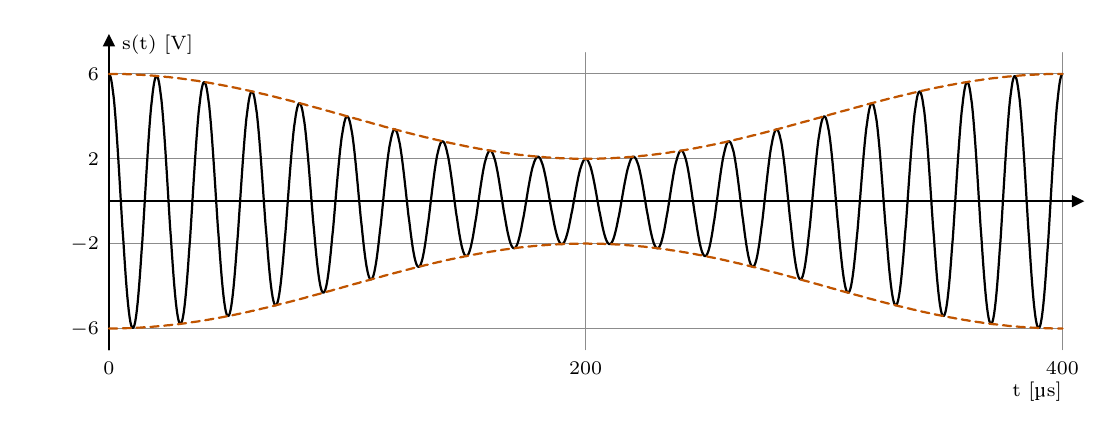
\begin{tikzpicture}[x=0.01985cm,y=-0.01985cm,line cap=round,line join=round]
\useasboundingbox (0,0) rectangle (680,240);
\path[draw=black!45,line width=0.35pt] (52,206) -- (52,16);
\path[draw=black!45,line width=0.35pt] (357,206) -- (357,16);
\path[draw=black!45,line width=0.35pt] (662,206) -- (662,16);
\path[draw=black!45,line width=0.35pt] (52,29.6) -- (662,29.6);
\path[draw=black!45,line width=0.35pt] (52,83.9) -- (662,83.9);
\path[draw=black!45,line width=0.35pt] (52,138.1) -- (662,138.1);
\path[draw=black!45,line width=0.35pt] (52,192.4) -- (662,192.4);
\path[draw=black,line width=0.7pt] (52,111) -- (670,111);
\path[fill=black,draw=none] (676,111) -- (668,107) -- (668,115) -- cycle;
\path[draw=black,line width=0.7pt] (52,206) -- (52,10);
\path[fill=black,draw=none] (52,4) -- (48,12) -- (56,12) -- cycle;
\node[anchor=base,inner sep=0pt,font=\scriptsize] at (52,222) {0};
\node[anchor=base,inner sep=0pt,font=\scriptsize] at (357,222) {200};
\node[anchor=base,inner sep=0pt,font=\scriptsize] at (662,222) {400};
\node[anchor=base east,inner sep=0pt,font=\scriptsize] at (46,33.6) {6};
\node[anchor=base east,inner sep=0pt,font=\scriptsize] at (46,87.9) {2};
\node[anchor=base east,inner sep=0pt,font=\scriptsize] at (46,142.1) {$-$2};
\node[anchor=base east,inner sep=0pt,font=\scriptsize] at (46,196.4) {$-$6};
\node[anchor=base east,inner sep=0pt,font=\scriptsize] at (662,236) {t [\textmu{}s]};
\node[anchor=base west,inner sep=0pt,font=\scriptsize] at (60,14) {s(t) [V]};
\path[draw=black,line width=0.8pt] (52,29.6) -- (52.5,30) -- (53,31.4) -- (53.5,33.6) -- (54,36.6) -- (54.5,40.5) -- (55.1,45.1) -- (55.6,50.5) -- (56.1,56.5) -- (56.6,63.2) -- (57.1,70.3) -- (57.6,77.9) -- (58.1,85.9) -- (58.6,94.1) -- (59.1,102.5) -- (59.6,111) -- (60.1,119.5) -- (60.6,127.9) -- (61.2,136.1) -- (61.7,144.1) -- (62.2,151.6) -- (62.7,158.8) -- (63.2,165.4) -- (63.7,171.4) -- (64.2,176.7) -- (64.7,181.3) -- (65.2,185.2) -- (65.7,188.2) -- (66.2,190.4) -- (66.7,191.7) -- (67.3,192.1) -- (67.8,191.6) -- (68.3,190.3) -- (68.8,188.1) -- (69.3,185) -- (69.8,181.1) -- (70.3,176.5) -- (70.8,171.1) -- (71.3,165.1) -- (71.8,158.5) -- (72.3,151.4) -- (72.8,143.9) -- (73.4,136) -- (73.9,127.8) -- (74.4,119.4) -- (74.9,111) -- (75.4,102.6) -- (75.9,94.2) -- (76.4,86.1) -- (76.9,78.2) -- (77.4,70.7) -- (77.9,63.7) -- (78.4,57.2) -- (78.9,51.3) -- (79.5,46) -- (80,41.4) -- (80.5,37.7) -- (81,34.7) -- (81.5,32.6) -- (82,31.3) -- (82.5,30.9) -- (83,31.4) -- (83.5,32.7) -- (84,34.9) -- (84.5,38) -- (85,41.8) -- (85.6,46.4) -- (86.1,51.7) -- (86.6,57.7) -- (87.1,64.2) -- (87.6,71.2) -- (88.1,78.6) -- (88.6,86.4) -- (89.1,94.5) -- (89.6,102.7) -- (90.1,111) -- (90.6,119.3) -- (91.1,127.5) -- (91.7,135.5) -- (92.2,143.2) -- (92.7,150.5) -- (93.2,157.4) -- (93.7,163.8) -- (94.2,169.6) -- (94.7,174.8) -- (95.2,179.2) -- (95.7,182.9) -- (96.2,185.8) -- (96.7,187.9) -- (97.2,189.1) -- (97.8,189.5) -- (98.3,189) -- (98.8,187.6) -- (99.3,185.4) -- (99.8,182.4) -- (100.3,178.7) -- (100.8,174.2) -- (101.3,169) -- (101.8,163.1) -- (102.3,156.8) -- (102.8,149.9) -- (103.3,142.6) -- (103.9,135) -- (104.4,127.1) -- (104.9,119.1) -- (105.4,111) -- (105.9,102.9) -- (106.4,94.9) -- (106.9,87.1) -- (107.4,79.6) -- (107.9,72.5) -- (108.4,65.8) -- (108.9,59.5) -- (109.4,53.9) -- (110,48.9) -- (110.5,44.6) -- (111,41) -- (111.5,38.3) -- (112,36.3) -- (112.5,35.1) -- (113,34.8) -- (113.5,35.3) -- (114,36.6) -- (114.5,38.7) -- (115,41.7) -- (115.5,45.3) -- (116.1,49.7) -- (116.6,54.8) -- (117.1,60.4) -- (117.6,66.6) -- (118.1,73.3) -- (118.6,80.4) -- (119.1,87.8) -- (119.6,95.4) -- (120.1,103.2) -- (120.6,111) -- (121.1,118.8) -- (121.6,126.5) -- (122.2,134.1) -- (122.7,141.3) -- (123.2,148.2) -- (123.7,154.7) -- (124.2,160.7) -- (124.7,166.1) -- (125.2,170.9) -- (125.7,175.1) -- (126.2,178.5) -- (126.7,181.2) -- (127.2,183.1) -- (127.7,184.2) -- (128.3,184.5) -- (128.8,184) -- (129.3,182.7) -- (129.8,180.6) -- (130.3,177.8) -- (130.8,174.2) -- (131.3,170) -- (131.8,165.1) -- (132.3,159.6) -- (132.8,153.6) -- (133.3,147.2) -- (133.8,140.4) -- (134.4,133.3) -- (134.9,126) -- (135.4,118.5) -- (135.9,111) -- (136.4,103.5) -- (136.9,96.1) -- (137.4,88.9) -- (137.9,81.9) -- (138.4,75.3) -- (138.9,69.1) -- (139.4,63.4) -- (139.9,58.2) -- (140.5,53.6) -- (141,49.7) -- (141.5,46.4) -- (142,43.9) -- (142.5,42.1) -- (143,41) -- (143.5,40.8) -- (144,41.3) -- (144.5,42.5) -- (145,44.5) -- (145.5,47.3) -- (146,50.7) -- (146.6,54.7) -- (147.1,59.4) -- (147.6,64.6) -- (148.1,70.3) -- (148.6,76.5) -- (149.1,83) -- (149.6,89.7) -- (150.1,96.7) -- (150.6,103.8) -- (151.1,111) -- (151.6,118.1) -- (152.1,125.2) -- (152.7,132) -- (153.2,138.6) -- (153.7,144.9) -- (154.2,150.8) -- (154.7,156.2) -- (155.2,161.2) -- (155.7,165.5) -- (156.2,169.2) -- (156.7,172.3) -- (157.2,174.7) -- (157.7,176.4) -- (158.2,177.4) -- (158.8,177.6) -- (159.3,177.1) -- (159.8,175.9) -- (160.3,174) -- (160.8,171.4) -- (161.3,168.1) -- (161.8,164.3) -- (162.3,159.8) -- (162.8,154.9) -- (163.3,149.5) -- (163.8,143.7) -- (164.3,137.5) -- (164.9,131.1) -- (165.4,124.5) -- (165.9,117.8) -- (166.4,111) -- (166.9,104.3) -- (167.4,97.6) -- (167.9,91.1) -- (168.4,84.9) -- (168.9,79) -- (169.4,73.5) -- (169.9,68.3) -- (170.4,63.7) -- (171,59.6) -- (171.5,56.1) -- (172,53.3) -- (172.5,51) -- (173,49.4) -- (173.5,48.5) -- (174,48.3) -- (174.5,48.8) -- (175,50) -- (175.5,51.8) -- (176,54.2) -- (176.5,57.3) -- (177.1,61) -- (177.6,65.1) -- (178.1,69.8) -- (178.6,74.9) -- (179.1,80.3) -- (179.6,86.1) -- (180.1,92.1) -- (180.6,98.3) -- (181.1,104.6) -- (181.6,111) -- (182.1,117.3) -- (182.6,123.5) -- (183.2,129.6) -- (183.7,135.4) -- (184.2,141) -- (184.7,146.1) -- (185.2,150.9) -- (185.7,155.2) -- (186.2,159) -- (186.7,162.3) -- (187.2,165) -- (187.7,167.1) -- (188.2,168.5) -- (188.7,169.4) -- (189.3,169.5) -- (189.8,169.1) -- (190.3,168) -- (190.8,166.3) -- (191.3,164) -- (191.8,161.1) -- (192.3,157.7) -- (192.8,153.8) -- (193.3,149.4) -- (193.8,144.7) -- (194.3,139.6) -- (194.8,134.2) -- (195.4,128.6) -- (195.9,122.8) -- (196.4,116.9) -- (196.9,111) -- (197.4,105.1) -- (197.9,99.3) -- (198.4,93.7) -- (198.9,88.3) -- (199.4,83.1) -- (199.9,78.3) -- (200.4,73.9) -- (200.9,69.9) -- (201.5,66.4) -- (202,63.4) -- (202.5,60.9) -- (203,59) -- (203.5,57.6) -- (204,56.9) -- (204.5,56.7) -- (205,57.2) -- (205.5,58.2) -- (206,59.8) -- (206.5,61.9) -- (207,64.6) -- (207.6,67.8) -- (208.1,71.4) -- (208.6,75.4) -- (209.1,79.8) -- (209.6,84.6) -- (210.1,89.6) -- (210.6,94.8) -- (211.1,100.1) -- (211.6,105.5) -- (212.1,111) -- (212.6,116.4) -- (213.1,121.8) -- (213.7,127) -- (214.2,132) -- (214.7,136.7) -- (215.2,141.2) -- (215.7,145.2) -- (216.2,148.9) -- (216.7,152.2) -- (217.2,154.9) -- (217.7,157.2) -- (218.2,159) -- (218.7,160.2) -- (219.2,160.9) -- (219.8,161) -- (220.3,160.6) -- (220.8,159.7) -- (221.3,158.2) -- (221.8,156.2) -- (222.3,153.7) -- (222.8,150.8) -- (223.3,147.5) -- (223.8,143.7) -- (224.3,139.7) -- (224.8,135.3) -- (225.3,130.7) -- (225.9,125.9) -- (226.4,121) -- (226.9,116) -- (227.4,111) -- (227.9,106) -- (228.4,101.1) -- (228.9,96.3) -- (229.4,91.7) -- (229.9,87.4) -- (230.4,83.3) -- (230.9,79.6) -- (231.4,76.2) -- (232,73.2) -- (232.5,70.7) -- (233,68.6) -- (233.5,67) -- (234,65.8) -- (234.5,65.2) -- (235,65.1) -- (235.5,65.5) -- (236,66.4) -- (236.5,67.7) -- (237,69.6) -- (237.5,71.8) -- (238.1,74.5) -- (238.6,77.6) -- (239.1,81) -- (239.6,84.7) -- (240.1,88.7) -- (240.6,92.9) -- (241.1,97.3) -- (241.6,101.8) -- (242.1,106.4) -- (242.6,111) -- (243.1,115.6) -- (243.6,120.1) -- (244.2,124.4) -- (244.7,128.6) -- (245.2,132.6) -- (245.7,136.3) -- (246.2,139.8) -- (246.7,142.8) -- (247.2,145.6) -- (247.7,147.9) -- (248.2,149.8) -- (248.7,151.3) -- (249.2,152.3) -- (249.7,152.9) -- (250.3,153) -- (250.8,152.6) -- (251.3,151.8) -- (251.8,150.5) -- (252.3,148.9) -- (252.8,146.8) -- (253.3,144.3) -- (253.8,141.5) -- (254.3,138.4) -- (254.8,135) -- (255.3,131.4) -- (255.8,127.5) -- (256.4,123.5) -- (256.9,119.4) -- (257.4,115.2) -- (257.9,111) -- (258.4,106.8) -- (258.9,102.7) -- (259.4,98.7) -- (259.9,94.9) -- (260.4,91.2) -- (260.9,87.9) -- (261.4,84.7) -- (261.9,81.9) -- (262.5,79.4) -- (263,77.3) -- (263.5,75.6) -- (264,74.2) -- (264.5,73.3) -- (265,72.8) -- (265.5,72.7) -- (266,73) -- (266.5,73.7) -- (267,74.9) -- (267.5,76.4) -- (268,78.3) -- (268.5,80.5) -- (269.1,83.1) -- (269.6,86) -- (270.1,89.1) -- (270.6,92.4) -- (271.1,95.9) -- (271.6,99.6) -- (272.1,103.3) -- (272.6,107.2) -- (273.1,111) -- (273.6,114.8) -- (274.1,118.6) -- (274.7,122.2) -- (275.2,125.7) -- (275.7,129.1) -- (276.2,132.2) -- (276.7,135) -- (277.2,137.6) -- (277.7,139.9) -- (278.2,141.8) -- (278.7,143.4) -- (279.2,144.7) -- (279.7,145.5) -- (280.2,146) -- (280.8,146.1) -- (281.3,145.8) -- (281.8,145.1) -- (282.3,144.1) -- (282.8,142.7) -- (283.3,141) -- (283.8,138.9) -- (284.3,136.6) -- (284.8,134) -- (285.3,131.1) -- (285.8,128.1) -- (286.3,124.8) -- (286.9,121.5) -- (287.4,118) -- (287.9,114.5) -- (288.4,111) -- (288.9,107.5) -- (289.4,104) -- (289.9,100.7) -- (290.4,97.5) -- (290.9,94.4) -- (291.4,91.5) -- (291.9,88.9) -- (292.4,86.5) -- (293,84.4) -- (293.5,82.6) -- (294,81.2) -- (294.5,80) -- (295,79.2) -- (295.5,78.8) -- (296,78.7) -- (296.5,78.9) -- (297,79.5) -- (297.5,80.5) -- (298,81.8) -- (298.5,83.4) -- (299.1,85.2) -- (299.6,87.4) -- (300.1,89.8) -- (300.6,92.4) -- (301.1,95.2) -- (301.6,98.2) -- (302.1,101.3) -- (302.6,104.5) -- (303.1,107.7) -- (303.6,111) -- (304.1,114.2) -- (304.6,117.4) -- (305.2,120.6) -- (305.7,123.5) -- (306.2,126.4) -- (306.7,129.1) -- (307.2,131.5) -- (307.7,133.7) -- (308.2,135.7) -- (308.7,137.4) -- (309.2,138.7) -- (309.7,139.8) -- (310.2,140.6) -- (310.7,141) -- (311.3,141.1) -- (311.8,140.9) -- (312.3,140.3) -- (312.8,139.4) -- (313.3,138.3) -- (313.8,136.8) -- (314.3,135) -- (314.8,133) -- (315.3,130.8) -- (315.8,128.4) -- (316.3,125.7) -- (316.8,123) -- (317.4,120.1) -- (317.9,117.1) -- (318.4,114.1) -- (318.9,111) -- (319.4,108) -- (319.9,104.9) -- (320.4,102) -- (320.9,99.2) -- (321.4,96.5) -- (321.9,94) -- (322.4,91.7) -- (322.9,89.6) -- (323.5,87.7) -- (324,86.1) -- (324.5,84.8) -- (325,83.8) -- (325.5,83.1) -- (326,82.6) -- (326.5,82.5) -- (327,82.7) -- (327.5,83.2) -- (328,84) -- (328.5,85.1) -- (329,86.5) -- (329.6,88.2) -- (330.1,90.1) -- (330.6,92.2) -- (331.1,94.5) -- (331.6,97) -- (332.1,99.6) -- (332.6,102.3) -- (333.1,105.2) -- (333.6,108.1) -- (334.1,111) -- (334.6,113.9) -- (335.1,116.8) -- (335.7,119.6) -- (336.2,122.3) -- (336.7,124.9) -- (337.2,127.3) -- (337.7,129.5) -- (338.2,131.5) -- (338.7,133.3) -- (339.2,134.9) -- (339.7,136.2) -- (340.2,137.2) -- (340.7,137.9) -- (341.2,138.3) -- (341.8,138.5) -- (342.3,138.3) -- (342.8,137.8) -- (343.3,137.1) -- (343.8,136) -- (344.3,134.7) -- (344.8,133.1) -- (345.3,131.3) -- (345.8,129.3) -- (346.3,127.1) -- (346.8,124.6) -- (347.3,122.1) -- (347.8,119.4) -- (348.4,116.7) -- (348.9,113.8) -- (349.4,111) -- (349.9,108.2) -- (350.4,105.3) -- (350.9,102.6) -- (351.4,99.9) -- (351.9,97.4) -- (352.4,95) -- (352.9,92.8) -- (353.4,90.8) -- (354,89) -- (354.5,87.5) -- (355,86.2) -- (355.5,85.2) -- (356,84.4) -- (356.5,84) -- (357,83.9) -- (357.5,84) -- (358,84.4) -- (358.5,85.2) -- (359,86.2) -- (359.5,87.5) -- (360.1,89) -- (360.6,90.8) -- (361.1,92.8) -- (361.6,95) -- (362.1,97.4) -- (362.6,99.9) -- (363.1,102.6) -- (363.6,105.3) -- (364.1,108.2) -- (364.6,111) -- (365.1,113.8) -- (365.6,116.7) -- (366.2,119.4) -- (366.7,122.1) -- (367.2,124.6) -- (367.7,127.1) -- (368.2,129.3) -- (368.7,131.3) -- (369.2,133.1) -- (369.7,134.7) -- (370.2,136) -- (370.7,137.1) -- (371.2,137.8) -- (371.7,138.3) -- (372.3,138.5) -- (372.8,138.3) -- (373.3,137.9) -- (373.8,137.2) -- (374.3,136.2) -- (374.8,134.9) -- (375.3,133.3) -- (375.8,131.5) -- (376.3,129.5) -- (376.8,127.3) -- (377.3,124.9) -- (377.8,122.3) -- (378.4,119.6) -- (378.9,116.8) -- (379.4,113.9) -- (379.9,111) -- (380.4,108.1) -- (380.9,105.2) -- (381.4,102.3) -- (381.9,99.6) -- (382.4,97) -- (382.9,94.5) -- (383.4,92.2) -- (383.9,90.1) -- (384.5,88.2) -- (385,86.5) -- (385.5,85.1) -- (386,84) -- (386.5,83.2) -- (387,82.7) -- (387.5,82.5) -- (388,82.6) -- (388.5,83.1) -- (389,83.8) -- (389.5,84.8) -- (390,86.1) -- (390.6,87.7) -- (391.1,89.6) -- (391.6,91.7) -- (392.1,94) -- (392.6,96.5) -- (393.1,99.2) -- (393.6,102) -- (394.1,104.9) -- (394.6,108) -- (395.1,111) -- (395.6,114.1) -- (396.1,117.1) -- (396.7,120.1) -- (397.2,123) -- (397.7,125.7) -- (398.2,128.4) -- (398.7,130.8) -- (399.2,133) -- (399.7,135) -- (400.2,136.8) -- (400.7,138.3) -- (401.2,139.4) -- (401.7,140.3) -- (402.2,140.9) -- (402.8,141.1) -- (403.3,141) -- (403.8,140.6) -- (404.3,139.8) -- (404.8,138.7) -- (405.3,137.4) -- (405.8,135.7) -- (406.3,133.7) -- (406.8,131.5) -- (407.3,129.1) -- (407.8,126.4) -- (408.3,123.5) -- (408.8,120.6) -- (409.4,117.4) -- (409.9,114.2) -- (410.4,111) -- (410.9,107.7) -- (411.4,104.5) -- (411.9,101.3) -- (412.4,98.2) -- (412.9,95.2) -- (413.4,92.4) -- (413.9,89.8) -- (414.4,87.4) -- (415,85.2) -- (415.5,83.4) -- (416,81.8) -- (416.5,80.5) -- (417,79.5) -- (417.5,78.9) -- (418,78.7) -- (418.5,78.8) -- (419,79.2) -- (419.5,80) -- (420,81.2) -- (420.5,82.6) -- (421.1,84.4) -- (421.6,86.5) -- (422.1,88.9) -- (422.6,91.5) -- (423.1,94.4) -- (423.6,97.5) -- (424.1,100.7) -- (424.6,104) -- (425.1,107.5) -- (425.6,111) -- (426.1,114.5) -- (426.6,118) -- (427.2,121.5) -- (427.7,124.8) -- (428.2,128.1) -- (428.7,131.1) -- (429.2,134) -- (429.7,136.6) -- (430.2,138.9) -- (430.7,141) -- (431.2,142.7) -- (431.7,144.1) -- (432.2,145.1) -- (432.7,145.8) -- (433.3,146.1) -- (433.8,146) -- (434.3,145.5) -- (434.8,144.7) -- (435.3,143.4) -- (435.8,141.8) -- (436.3,139.9) -- (436.8,137.6) -- (437.3,135) -- (437.8,132.2) -- (438.3,129.1) -- (438.8,125.7) -- (439.4,122.2) -- (439.9,118.6) -- (440.4,114.8) -- (440.9,111) -- (441.4,107.2) -- (441.9,103.3) -- (442.4,99.6) -- (442.9,95.9) -- (443.4,92.4) -- (443.9,89.1) -- (444.4,86) -- (444.9,83.1) -- (445.5,80.5) -- (446,78.3) -- (446.5,76.4) -- (447,74.9) -- (447.5,73.7) -- (448,73) -- (448.5,72.7) -- (449,72.8) -- (449.5,73.3) -- (450,74.2) -- (450.5,75.6) -- (451,77.3) -- (451.6,79.4) -- (452.1,81.9) -- (452.6,84.7) -- (453.1,87.9) -- (453.6,91.2) -- (454.1,94.9) -- (454.6,98.7) -- (455.1,102.7) -- (455.6,106.8) -- (456.1,111) -- (456.6,115.2) -- (457.1,119.4) -- (457.7,123.5) -- (458.2,127.5) -- (458.7,131.4) -- (459.2,135) -- (459.7,138.4) -- (460.2,141.5) -- (460.7,144.3) -- (461.2,146.8) -- (461.7,148.9) -- (462.2,150.5) -- (462.7,151.8) -- (463.2,152.6) -- (463.8,153) -- (464.3,152.9) -- (464.8,152.3) -- (465.3,151.3) -- (465.8,149.8) -- (466.3,147.9) -- (466.8,145.6) -- (467.3,142.8) -- (467.8,139.8) -- (468.3,136.3) -- (468.8,132.6) -- (469.3,128.6) -- (469.9,124.4) -- (470.4,120.1) -- (470.9,115.6) -- (471.4,111) -- (471.9,106.4) -- (472.4,101.8) -- (472.9,97.3) -- (473.4,92.9) -- (473.9,88.7) -- (474.4,84.7) -- (474.9,81) -- (475.4,77.6) -- (476,74.5) -- (476.5,71.8) -- (477,69.6) -- (477.5,67.7) -- (478,66.4) -- (478.5,65.5) -- (479,65.1) -- (479.5,65.2) -- (480,65.8) -- (480.5,67) -- (481,68.6) -- (481.5,70.7) -- (482.1,73.2) -- (482.6,76.2) -- (483.1,79.6) -- (483.6,83.3) -- (484.1,87.4) -- (484.6,91.7) -- (485.1,96.3) -- (485.6,101.1) -- (486.1,106) -- (486.6,111) -- (487.1,116) -- (487.6,121) -- (488.2,125.9) -- (488.7,130.7) -- (489.2,135.3) -- (489.7,139.7) -- (490.2,143.7) -- (490.7,147.5) -- (491.2,150.8) -- (491.7,153.7) -- (492.2,156.2) -- (492.7,158.2) -- (493.2,159.7) -- (493.7,160.6) -- (494.3,161) -- (494.8,160.9) -- (495.3,160.2) -- (495.8,159) -- (496.3,157.2) -- (496.8,154.9) -- (497.3,152.2) -- (497.8,148.9) -- (498.3,145.2) -- (498.8,141.2) -- (499.3,136.7) -- (499.8,132) -- (500.4,127) -- (500.9,121.8) -- (501.4,116.4) -- (501.9,111) -- (502.4,105.5) -- (502.9,100.1) -- (503.4,94.8) -- (503.9,89.6) -- (504.4,84.6) -- (504.9,79.8) -- (505.4,75.4) -- (505.9,71.4) -- (506.5,67.8) -- (507,64.6) -- (507.5,61.9) -- (508,59.8) -- (508.5,58.2) -- (509,57.2) -- (509.5,56.7) -- (510,56.9) -- (510.5,57.6) -- (511,59) -- (511.5,60.9) -- (512,63.4) -- (512.6,66.4) -- (513.1,69.9) -- (513.6,73.9) -- (514.1,78.3) -- (514.6,83.1) -- (515.1,88.3) -- (515.6,93.7) -- (516.1,99.3) -- (516.6,105.1) -- (517.1,111) -- (517.6,116.9) -- (518.1,122.8) -- (518.7,128.6) -- (519.2,134.2) -- (519.7,139.6) -- (520.2,144.7) -- (520.7,149.4) -- (521.2,153.8) -- (521.7,157.7) -- (522.2,161.1) -- (522.7,164) -- (523.2,166.3) -- (523.7,168) -- (524.2,169.1) -- (524.8,169.5) -- (525.3,169.4) -- (525.8,168.5) -- (526.3,167.1) -- (526.8,165) -- (527.3,162.3) -- (527.8,159) -- (528.3,155.2) -- (528.8,150.9) -- (529.3,146.1) -- (529.8,141) -- (530.3,135.4) -- (530.9,129.6) -- (531.4,123.5) -- (531.9,117.3) -- (532.4,111) -- (532.9,104.6) -- (533.4,98.3) -- (533.9,92.1) -- (534.4,86.1) -- (534.9,80.3) -- (535.4,74.9) -- (535.9,69.8) -- (536.4,65.1) -- (537,61) -- (537.5,57.3) -- (538,54.2) -- (538.5,51.8) -- (539,50) -- (539.5,48.8) -- (540,48.3) -- (540.5,48.5) -- (541,49.4) -- (541.5,51) -- (542,53.3) -- (542.5,56.1) -- (543.1,59.6) -- (543.6,63.7) -- (544.1,68.3) -- (544.6,73.5) -- (545.1,79) -- (545.6,84.9) -- (546.1,91.1) -- (546.6,97.6) -- (547.1,104.3) -- (547.6,111) -- (548.1,117.8) -- (548.6,124.5) -- (549.2,131.1) -- (549.7,137.5) -- (550.2,143.7) -- (550.7,149.5) -- (551.2,154.9) -- (551.7,159.8) -- (552.2,164.3) -- (552.7,168.1) -- (553.2,171.4) -- (553.7,174) -- (554.2,175.9) -- (554.7,177.1) -- (555.3,177.6) -- (555.8,177.4) -- (556.3,176.4) -- (556.8,174.7) -- (557.3,172.3) -- (557.8,169.2) -- (558.3,165.5) -- (558.8,161.2) -- (559.3,156.2) -- (559.8,150.8) -- (560.3,144.9) -- (560.8,138.6) -- (561.3,132) -- (561.9,125.2) -- (562.4,118.1) -- (562.9,111) -- (563.4,103.8) -- (563.9,96.7) -- (564.4,89.7) -- (564.9,83) -- (565.4,76.5) -- (565.9,70.3) -- (566.4,64.6) -- (566.9,59.4) -- (567.4,54.7) -- (568,50.7) -- (568.5,47.3) -- (569,44.5) -- (569.5,42.5) -- (570,41.3) -- (570.5,40.8) -- (571,41) -- (571.5,42.1) -- (572,43.9) -- (572.5,46.4) -- (573,49.7) -- (573.6,53.6) -- (574.1,58.2) -- (574.6,63.4) -- (575.1,69.1) -- (575.6,75.3) -- (576.1,81.9) -- (576.6,88.9) -- (577.1,96.1) -- (577.6,103.5) -- (578.1,111) -- (578.6,118.5) -- (579.1,126) -- (579.7,133.3) -- (580.2,140.4) -- (580.7,147.2) -- (581.2,153.6) -- (581.7,159.6) -- (582.2,165.1) -- (582.7,170) -- (583.2,174.2) -- (583.7,177.8) -- (584.2,180.6) -- (584.7,182.7) -- (585.2,184) -- (585.8,184.5) -- (586.3,184.2) -- (586.8,183.1) -- (587.3,181.2) -- (587.8,178.5) -- (588.3,175.1) -- (588.8,170.9) -- (589.3,166.1) -- (589.8,160.7) -- (590.3,154.7) -- (590.8,148.2) -- (591.3,141.3) -- (591.9,134.1) -- (592.4,126.5) -- (592.9,118.8) -- (593.4,111) -- (593.9,103.2) -- (594.4,95.4) -- (594.9,87.8) -- (595.4,80.4) -- (595.9,73.3) -- (596.4,66.6) -- (596.9,60.4) -- (597.4,54.8) -- (598,49.7) -- (598.5,45.3) -- (599,41.7) -- (599.5,38.7) -- (600,36.6) -- (600.5,35.3) -- (601,34.8) -- (601.5,35.1) -- (602,36.3) -- (602.5,38.3) -- (603,41) -- (603.5,44.6) -- (604.1,48.9) -- (604.6,53.9) -- (605.1,59.5) -- (605.6,65.8) -- (606.1,72.5) -- (606.6,79.6) -- (607.1,87.1) -- (607.6,94.9) -- (608.1,102.9) -- (608.6,111) -- (609.1,119.1) -- (609.6,127.1) -- (610.2,135) -- (610.7,142.6) -- (611.2,149.9) -- (611.7,156.8) -- (612.2,163.1) -- (612.7,169) -- (613.2,174.2) -- (613.7,178.7) -- (614.2,182.4) -- (614.7,185.4) -- (615.2,187.6) -- (615.7,189) -- (616.3,189.5) -- (616.8,189.1) -- (617.3,187.9) -- (617.8,185.8) -- (618.3,182.9) -- (618.8,179.2) -- (619.3,174.8) -- (619.8,169.6) -- (620.3,163.8) -- (620.8,157.4) -- (621.3,150.5) -- (621.8,143.2) -- (622.4,135.5) -- (622.9,127.5) -- (623.4,119.3) -- (623.9,111) -- (624.4,102.7) -- (624.9,94.5) -- (625.4,86.4) -- (625.9,78.6) -- (626.4,71.2) -- (626.9,64.2) -- (627.4,57.7) -- (627.9,51.7) -- (628.4,46.4) -- (629,41.8) -- (629.5,38) -- (630,34.9) -- (630.5,32.7) -- (631,31.4) -- (631.5,30.9) -- (632,31.3) -- (632.5,32.6) -- (633,34.7) -- (633.5,37.7) -- (634,41.4) -- (634.6,46) -- (635.1,51.3) -- (635.6,57.2) -- (636.1,63.7) -- (636.6,70.7) -- (637.1,78.2) -- (637.6,86.1) -- (638.1,94.2) -- (638.6,102.6) -- (639.1,111) -- (639.6,119.4) -- (640.1,127.8) -- (640.7,136) -- (641.2,143.9) -- (641.7,151.4) -- (642.2,158.5) -- (642.7,165.1) -- (643.2,171.1) -- (643.7,176.5) -- (644.2,181.1) -- (644.7,185) -- (645.2,188.1) -- (645.7,190.3) -- (646.2,191.6) -- (646.8,192.1) -- (647.3,191.7) -- (647.8,190.4) -- (648.3,188.2) -- (648.8,185.2) -- (649.3,181.3) -- (649.8,176.7) -- (650.3,171.4) -- (650.8,165.4) -- (651.3,158.8) -- (651.8,151.6) -- (652.3,144.1) -- (652.9,136.1) -- (653.4,127.9) -- (653.9,119.5) -- (654.4,111) -- (654.9,102.5) -- (655.4,94.1) -- (655.9,85.9) -- (656.4,77.9) -- (656.9,70.3) -- (657.4,63.2) -- (657.9,56.5) -- (658.4,50.5) -- (659,45.1) -- (659.5,40.5) -- (660,36.6) -- (660.5,33.6) -- (661,31.4) -- (661.5,30) -- (662,29.6);
\path[draw=cB,line width=0.8pt,dash pattern=on 3pt off 2pt] (52,29.6) -- (52.8,29.6) -- (53.5,29.6) -- (54.3,29.6) -- (55.1,29.6) -- (55.8,29.6) -- (56.6,29.6) -- (57.3,29.6) -- (58.1,29.6) -- (58.9,29.6) -- (59.6,29.7) -- (60.4,29.7) -- (61.2,29.7) -- (61.9,29.7) -- (62.7,29.7) -- (63.4,29.8) -- (64.2,29.8) -- (65,29.8) -- (65.7,29.8) -- (66.5,29.9) -- (67.3,29.9) -- (68,29.9) -- (68.8,30) -- (69.5,30) -- (70.3,30.1) -- (71.1,30.1) -- (71.8,30.1) -- (72.6,30.2) -- (73.4,30.2) -- (74.1,30.3) -- (74.9,30.3) -- (75.6,30.4) -- (76.4,30.4) -- (77.2,30.5) -- (77.9,30.5) -- (78.7,30.6) -- (79.5,30.6) -- (80.2,30.7) -- (81,30.8) -- (81.7,30.8) -- (82.5,30.9) -- (83.3,31) -- (84,31) -- (84.8,31.1) -- (85.6,31.2) -- (86.3,31.2) -- (87.1,31.3) -- (87.8,31.4) -- (88.6,31.5) -- (89.4,31.6) -- (90.1,31.6) -- (90.9,31.7) -- (91.7,31.8) -- (92.4,31.9) -- (93.2,32) -- (93.9,32.1) -- (94.7,32.2) -- (95.5,32.2) -- (96.2,32.3) -- (97,32.4) -- (97.8,32.5) -- (98.5,32.6) -- (99.3,32.7) -- (100,32.8) -- (100.8,32.9) -- (101.6,33) -- (102.3,33.1) -- (103.1,33.2) -- (103.9,33.4) -- (104.6,33.5) -- (105.4,33.6) -- (106.1,33.7) -- (106.9,33.8) -- (107.7,33.9) -- (108.4,34) -- (109.2,34.1) -- (110,34.3) -- (110.7,34.4) -- (111.5,34.5) -- (112.2,34.6) -- (113,34.8) -- (113.8,34.9) -- (114.5,35) -- (115.3,35.1) -- (116.1,35.3) -- (116.8,35.4) -- (117.6,35.5) -- (118.3,35.7) -- (119.1,35.8) -- (119.9,35.9) -- (120.6,36.1) -- (121.4,36.2) -- (122.2,36.4) -- (122.9,36.5) -- (123.7,36.6) -- (124.4,36.8) -- (125.2,36.9) -- (126,37.1) -- (126.7,37.2) -- (127.5,37.4) -- (128.3,37.5) -- (129,37.7) -- (129.8,37.8) -- (130.5,38) -- (131.3,38.1) -- (132.1,38.3) -- (132.8,38.4) -- (133.6,38.6) -- (134.4,38.8) -- (135.1,38.9) -- (135.9,39.1) -- (136.6,39.2) -- (137.4,39.4) -- (138.2,39.6) -- (138.9,39.7) -- (139.7,39.9) -- (140.5,40.1) -- (141.2,40.2) -- (142,40.4) -- (142.7,40.6) -- (143.5,40.8) -- (144.3,40.9) -- (145,41.1) -- (145.8,41.3) -- (146.6,41.5) -- (147.3,41.6) -- (148.1,41.8) -- (148.8,42) -- (149.6,42.2) -- (150.4,42.4) -- (151.1,42.5) -- (151.9,42.7) -- (152.7,42.9) -- (153.4,43.1) -- (154.2,43.3) -- (154.9,43.5) -- (155.7,43.6) -- (156.5,43.8) -- (157.2,44) -- (158,44.2) -- (158.8,44.4) -- (159.5,44.6) -- (160.3,44.8) -- (161,45) -- (161.8,45.2) -- (162.6,45.4) -- (163.3,45.5) -- (164.1,45.7) -- (164.9,45.9) -- (165.6,46.1) -- (166.4,46.3) -- (167.1,46.5) -- (167.9,46.7) -- (168.7,46.9) -- (169.4,47.1) -- (170.2,47.3) -- (171,47.5) -- (171.7,47.7) -- (172.5,47.9) -- (173.2,48.1) -- (174,48.3) -- (174.8,48.5) -- (175.5,48.7) -- (176.3,48.9) -- (177.1,49.1) -- (177.8,49.3) -- (178.6,49.6) -- (179.3,49.8) -- (180.1,50) -- (180.9,50.2) -- (181.6,50.4) -- (182.4,50.6) -- (183.2,50.8) -- (183.9,51) -- (184.7,51.2) -- (185.4,51.4) -- (186.2,51.6) -- (187,51.8) -- (187.7,52) -- (188.5,52.3) -- (189.3,52.5) -- (190,52.7) -- (190.8,52.9) -- (191.5,53.1) -- (192.3,53.3) -- (193.1,53.5) -- (193.8,53.7) -- (194.6,53.9) -- (195.4,54.2) -- (196.1,54.4) -- (196.9,54.6) -- (197.6,54.8) -- (198.4,55) -- (199.2,55.2) -- (199.9,55.4) -- (200.7,55.6) -- (201.5,55.9) -- (202.2,56.1) -- (203,56.3) -- (203.7,56.5) -- (204.5,56.7) -- (205.3,56.9) -- (206,57.1) -- (206.8,57.4) -- (207.6,57.6) -- (208.3,57.8) -- (209.1,58) -- (209.8,58.2) -- (210.6,58.4) -- (211.4,58.6) -- (212.1,58.8) -- (212.9,59.1) -- (213.7,59.3) -- (214.4,59.5) -- (215.2,59.7) -- (215.9,59.9) -- (216.7,60.1) -- (217.5,60.3) -- (218.2,60.5) -- (219,60.7) -- (219.8,61) -- (220.5,61.2) -- (221.3,61.4) -- (222,61.6) -- (222.8,61.8) -- (223.6,62) -- (224.3,62.2) -- (225.1,62.4) -- (225.9,62.6) -- (226.6,62.8) -- (227.4,63.1) -- (228.1,63.3) -- (228.9,63.5) -- (229.7,63.7) -- (230.4,63.9) -- (231.2,64.1) -- (232,64.3) -- (232.7,64.5) -- (233.5,64.7) -- (234.2,64.9) -- (235,65.1) -- (235.8,65.3) -- (236.5,65.5) -- (237.3,65.7) -- (238.1,65.9) -- (238.8,66.1) -- (239.6,66.3) -- (240.3,66.5) -- (241.1,66.7) -- (241.9,66.9) -- (242.6,67.1) -- (243.4,67.3) -- (244.2,67.5) -- (244.9,67.7) -- (245.7,67.9) -- (246.4,68.1) -- (247.2,68.3) -- (248,68.5) -- (248.7,68.7) -- (249.5,68.8) -- (250.3,69) -- (251,69.2) -- (251.8,69.4) -- (252.5,69.6) -- (253.3,69.8) -- (254.1,70) -- (254.8,70.2) -- (255.6,70.3) -- (256.4,70.5) -- (257.1,70.7) -- (257.9,70.9) -- (258.6,71.1) -- (259.4,71.3) -- (260.2,71.4) -- (260.9,71.6) -- (261.7,71.8) -- (262.5,72) -- (263.2,72.1) -- (264,72.3) -- (264.7,72.5) -- (265.5,72.7) -- (266.3,72.8) -- (267,73) -- (267.8,73.2) -- (268.5,73.4) -- (269.3,73.5) -- (270.1,73.7) -- (270.8,73.9) -- (271.6,74) -- (272.4,74.2) -- (273.1,74.3) -- (273.9,74.5) -- (274.7,74.7) -- (275.4,74.8) -- (276.2,75) -- (276.9,75.1) -- (277.7,75.3) -- (278.5,75.4) -- (279.2,75.6) -- (280,75.8) -- (280.8,75.9) -- (281.5,76.1) -- (282.3,76.2) -- (283,76.4) -- (283.8,76.5) -- (284.6,76.6) -- (285.3,76.8) -- (286.1,76.9) -- (286.9,77.1) -- (287.6,77.2) -- (288.4,77.4) -- (289.1,77.5) -- (289.9,77.6) -- (290.7,77.8) -- (291.4,77.9) -- (292.2,78) -- (293,78.2) -- (293.7,78.3) -- (294.5,78.4) -- (295.2,78.5) -- (296,78.7) -- (296.8,78.8) -- (297.5,78.9) -- (298.3,79) -- (299.1,79.2) -- (299.8,79.3) -- (300.6,79.4) -- (301.3,79.5) -- (302.1,79.6) -- (302.9,79.7) -- (303.6,79.9) -- (304.4,80) -- (305.2,80.1) -- (305.9,80.2) -- (306.7,80.3) -- (307.4,80.4) -- (308.2,80.5) -- (309,80.6) -- (309.7,80.7) -- (310.5,80.8) -- (311.3,80.9) -- (312,81) -- (312.8,81.1) -- (313.5,81.2) -- (314.3,81.3) -- (315.1,81.4) -- (315.8,81.5) -- (316.6,81.5) -- (317.4,81.6) -- (318.1,81.7) -- (318.9,81.8) -- (319.6,81.9) -- (320.4,82) -- (321.2,82) -- (321.9,82.1) -- (322.7,82.2) -- (323.5,82.3) -- (324.2,82.3) -- (325,82.4) -- (325.7,82.5) -- (326.5,82.5) -- (327.3,82.6) -- (328,82.7) -- (328.8,82.7) -- (329.6,82.8) -- (330.3,82.8) -- (331.1,82.9) -- (331.8,83) -- (332.6,83) -- (333.4,83.1) -- (334.1,83.1) -- (334.9,83.2) -- (335.7,83.2) -- (336.4,83.2) -- (337.2,83.3) -- (337.9,83.3) -- (338.7,83.4) -- (339.5,83.4) -- (340.2,83.5) -- (341,83.5) -- (341.8,83.5) -- (342.5,83.6) -- (343.3,83.6) -- (344,83.6) -- (344.8,83.6) -- (345.6,83.7) -- (346.3,83.7) -- (347.1,83.7) -- (347.8,83.7) -- (348.6,83.8) -- (349.4,83.8) -- (350.1,83.8) -- (350.9,83.8) -- (351.7,83.8) -- (352.4,83.8) -- (353.2,83.8) -- (354,83.8) -- (354.7,83.8) -- (355.5,83.9) -- (356.2,83.9) -- (357,83.9) -- (357.8,83.9) -- (358.5,83.9) -- (359.3,83.8) -- (360.1,83.8) -- (360.8,83.8) -- (361.6,83.8) -- (362.3,83.8) -- (363.1,83.8) -- (363.9,83.8) -- (364.6,83.8) -- (365.4,83.8) -- (366.2,83.7) -- (366.9,83.7) -- (367.7,83.7) -- (368.4,83.7) -- (369.2,83.6) -- (370,83.6) -- (370.7,83.6) -- (371.5,83.6) -- (372.3,83.5) -- (373,83.5) -- (373.8,83.5) -- (374.5,83.4) -- (375.3,83.4) -- (376.1,83.3) -- (376.8,83.3) -- (377.6,83.2) -- (378.4,83.2) -- (379.1,83.2) -- (379.9,83.1) -- (380.6,83.1) -- (381.4,83) -- (382.2,83) -- (382.9,82.9) -- (383.7,82.8) -- (384.5,82.8) -- (385.2,82.7) -- (386,82.7) -- (386.7,82.6) -- (387.5,82.5) -- (388.3,82.5) -- (389,82.4) -- (389.8,82.3) -- (390.6,82.3) -- (391.3,82.2) -- (392.1,82.1) -- (392.8,82) -- (393.6,82) -- (394.4,81.9) -- (395.1,81.8) -- (395.9,81.7) -- (396.7,81.6) -- (397.4,81.5) -- (398.2,81.5) -- (398.9,81.4) -- (399.7,81.3) -- (400.5,81.2) -- (401.2,81.1) -- (402,81) -- (402.8,80.9) -- (403.5,80.8) -- (404.3,80.7) -- (405,80.6) -- (405.8,80.5) -- (406.6,80.4) -- (407.3,80.3) -- (408.1,80.2) -- (408.8,80.1) -- (409.6,80) -- (410.4,79.9) -- (411.1,79.7) -- (411.9,79.6) -- (412.7,79.5) -- (413.4,79.4) -- (414.2,79.3) -- (415,79.2) -- (415.7,79) -- (416.5,78.9) -- (417.2,78.8) -- (418,78.7) -- (418.8,78.5) -- (419.5,78.4) -- (420.3,78.3) -- (421.1,78.2) -- (421.8,78) -- (422.6,77.9) -- (423.3,77.8) -- (424.1,77.6) -- (424.9,77.5) -- (425.6,77.4) -- (426.4,77.2) -- (427.2,77.1) -- (427.9,76.9) -- (428.7,76.8) -- (429.4,76.6) -- (430.2,76.5) -- (431,76.4) -- (431.7,76.2) -- (432.5,76.1) -- (433.3,75.9) -- (434,75.8) -- (434.8,75.6) -- (435.5,75.4) -- (436.3,75.3) -- (437.1,75.1) -- (437.8,75) -- (438.6,74.8) -- (439.4,74.7) -- (440.1,74.5) -- (440.9,74.3) -- (441.6,74.2) -- (442.4,74) -- (443.2,73.9) -- (443.9,73.7) -- (444.7,73.5) -- (445.5,73.4) -- (446.2,73.2) -- (447,73) -- (447.7,72.8) -- (448.5,72.7) -- (449.3,72.5) -- (450,72.3) -- (450.8,72.1) -- (451.6,72) -- (452.3,71.8) -- (453.1,71.6) -- (453.8,71.4) -- (454.6,71.3) -- (455.4,71.1) -- (456.1,70.9) -- (456.9,70.7) -- (457.7,70.5) -- (458.4,70.3) -- (459.2,70.2) -- (459.9,70) -- (460.7,69.8) -- (461.5,69.6) -- (462.2,69.4) -- (463,69.2) -- (463.8,69) -- (464.5,68.8) -- (465.3,68.7) -- (466,68.5) -- (466.8,68.3) -- (467.6,68.1) -- (468.3,67.9) -- (469.1,67.7) -- (469.9,67.5) -- (470.6,67.3) -- (471.4,67.1) -- (472.1,66.9) -- (472.9,66.7) -- (473.7,66.5) -- (474.4,66.3) -- (475.2,66.1) -- (476,65.9) -- (476.7,65.7) -- (477.5,65.5) -- (478.2,65.3) -- (479,65.1) -- (479.8,64.9) -- (480.5,64.7) -- (481.3,64.5) -- (482.1,64.3) -- (482.8,64.1) -- (483.6,63.9) -- (484.3,63.7) -- (485.1,63.5) -- (485.9,63.3) -- (486.6,63.1) -- (487.4,62.8) -- (488.2,62.6) -- (488.9,62.4) -- (489.7,62.2) -- (490.4,62) -- (491.2,61.8) -- (492,61.6) -- (492.7,61.4) -- (493.5,61.2) -- (494.3,61) -- (495,60.7) -- (495.8,60.5) -- (496.5,60.3) -- (497.3,60.1) -- (498.1,59.9) -- (498.8,59.7) -- (499.6,59.5) -- (500.4,59.3) -- (501.1,59.1) -- (501.9,58.8) -- (502.6,58.6) -- (503.4,58.4) -- (504.2,58.2) -- (504.9,58) -- (505.7,57.8) -- (506.5,57.6) -- (507.2,57.4) -- (508,57.1) -- (508.7,56.9) -- (509.5,56.7) -- (510.3,56.5) -- (511,56.3) -- (511.8,56.1) -- (512.6,55.9) -- (513.3,55.6) -- (514.1,55.4) -- (514.8,55.2) -- (515.6,55) -- (516.4,54.8) -- (517.1,54.6) -- (517.9,54.4) -- (518.7,54.2) -- (519.4,53.9) -- (520.2,53.7) -- (520.9,53.5) -- (521.7,53.3) -- (522.5,53.1) -- (523.2,52.9) -- (524,52.7) -- (524.8,52.5) -- (525.5,52.3) -- (526.3,52) -- (527,51.8) -- (527.8,51.6) -- (528.6,51.4) -- (529.3,51.2) -- (530.1,51) -- (530.9,50.8) -- (531.6,50.6) -- (532.4,50.4) -- (533.1,50.2) -- (533.9,50) -- (534.7,49.8) -- (535.4,49.6) -- (536.2,49.3) -- (537,49.1) -- (537.7,48.9) -- (538.5,48.7) -- (539.2,48.5) -- (540,48.3) -- (540.8,48.1) -- (541.5,47.9) -- (542.3,47.7) -- (543.1,47.5) -- (543.8,47.3) -- (544.6,47.1) -- (545.3,46.9) -- (546.1,46.7) -- (546.9,46.5) -- (547.6,46.3) -- (548.4,46.1) -- (549.2,45.9) -- (549.9,45.7) -- (550.7,45.5) -- (551.4,45.4) -- (552.2,45.2) -- (553,45) -- (553.7,44.8) -- (554.5,44.6) -- (555.3,44.4) -- (556,44.2) -- (556.8,44) -- (557.5,43.8) -- (558.3,43.6) -- (559.1,43.5) -- (559.8,43.3) -- (560.6,43.1) -- (561.3,42.9) -- (562.1,42.7) -- (562.9,42.5) -- (563.6,42.4) -- (564.4,42.2) -- (565.2,42) -- (565.9,41.8) -- (566.7,41.6) -- (567.4,41.5) -- (568.2,41.3) -- (569,41.1) -- (569.7,40.9) -- (570.5,40.8) -- (571.3,40.6) -- (572,40.4) -- (572.8,40.2) -- (573.6,40.1) -- (574.3,39.9) -- (575.1,39.7) -- (575.8,39.6) -- (576.6,39.4) -- (577.4,39.2) -- (578.1,39.1) -- (578.9,38.9) -- (579.7,38.8) -- (580.4,38.6) -- (581.2,38.4) -- (581.9,38.3) -- (582.7,38.1) -- (583.5,38) -- (584.2,37.8) -- (585,37.7) -- (585.8,37.5) -- (586.5,37.4) -- (587.3,37.2) -- (588,37.1) -- (588.8,36.9) -- (589.6,36.8) -- (590.3,36.6) -- (591.1,36.5) -- (591.9,36.4) -- (592.6,36.2) -- (593.4,36.1) -- (594.1,35.9) -- (594.9,35.8) -- (595.7,35.7) -- (596.4,35.5) -- (597.2,35.4) -- (598,35.3) -- (598.7,35.1) -- (599.5,35) -- (600.2,34.9) -- (601,34.8) -- (601.8,34.6) -- (602.5,34.5) -- (603.3,34.4) -- (604.1,34.3) -- (604.8,34.1) -- (605.6,34) -- (606.3,33.9) -- (607.1,33.8) -- (607.9,33.7) -- (608.6,33.6) -- (609.4,33.5) -- (610.2,33.4) -- (610.9,33.2) -- (611.7,33.1) -- (612.4,33) -- (613.2,32.9) -- (614,32.8) -- (614.7,32.7) -- (615.5,32.6) -- (616.3,32.5) -- (617,32.4) -- (617.8,32.3) -- (618.5,32.2) -- (619.3,32.2) -- (620.1,32.1) -- (620.8,32) -- (621.6,31.9) -- (622.4,31.8) -- (623.1,31.7) -- (623.9,31.6) -- (624.6,31.6) -- (625.4,31.5) -- (626.2,31.4) -- (626.9,31.3) -- (627.7,31.2) -- (628.4,31.2) -- (629.2,31.1) -- (630,31) -- (630.7,31) -- (631.5,30.9) -- (632.3,30.8) -- (633,30.8) -- (633.8,30.7) -- (634.6,30.6) -- (635.3,30.6) -- (636.1,30.5) -- (636.8,30.5) -- (637.6,30.4) -- (638.4,30.4) -- (639.1,30.3) -- (639.9,30.3) -- (640.7,30.2) -- (641.4,30.2) -- (642.2,30.1) -- (642.9,30.1) -- (643.7,30.1) -- (644.5,30) -- (645.2,30) -- (646,29.9) -- (646.8,29.9) -- (647.5,29.9) -- (648.3,29.8) -- (649,29.8) -- (649.8,29.8) -- (650.6,29.8) -- (651.3,29.7) -- (652.1,29.7) -- (652.9,29.7) -- (653.6,29.7) -- (654.4,29.7) -- (655.1,29.6) -- (655.9,29.6) -- (656.7,29.6) -- (657.4,29.6) -- (658.2,29.6) -- (659,29.6) -- (659.7,29.6) -- (660.5,29.6) -- (661.2,29.6) -- (662,29.6);
\path[draw=cB,line width=0.8pt,dash pattern=on 3pt off 2pt] (52,192.4) -- (52.8,192.4) -- (53.5,192.4) -- (54.3,192.4) -- (55.1,192.4) -- (55.8,192.4) -- (56.6,192.4) -- (57.3,192.4) -- (58.1,192.4) -- (58.9,192.4) -- (59.6,192.3) -- (60.4,192.3) -- (61.2,192.3) -- (61.9,192.3) -- (62.7,192.3) -- (63.4,192.2) -- (64.2,192.2) -- (65,192.2) -- (65.7,192.2) -- (66.5,192.1) -- (67.3,192.1) -- (68,192.1) -- (68.8,192) -- (69.5,192) -- (70.3,191.9) -- (71.1,191.9) -- (71.8,191.9) -- (72.6,191.8) -- (73.4,191.8) -- (74.1,191.7) -- (74.9,191.7) -- (75.6,191.6) -- (76.4,191.6) -- (77.2,191.5) -- (77.9,191.5) -- (78.7,191.4) -- (79.5,191.4) -- (80.2,191.3) -- (81,191.2) -- (81.7,191.2) -- (82.5,191.1) -- (83.3,191) -- (84,191) -- (84.8,190.9) -- (85.6,190.8) -- (86.3,190.8) -- (87.1,190.7) -- (87.8,190.6) -- (88.6,190.5) -- (89.4,190.4) -- (90.1,190.4) -- (90.9,190.3) -- (91.7,190.2) -- (92.4,190.1) -- (93.2,190) -- (93.9,189.9) -- (94.7,189.8) -- (95.5,189.8) -- (96.2,189.7) -- (97,189.6) -- (97.8,189.5) -- (98.5,189.4) -- (99.3,189.3) -- (100,189.2) -- (100.8,189.1) -- (101.6,189) -- (102.3,188.9) -- (103.1,188.8) -- (103.9,188.6) -- (104.6,188.5) -- (105.4,188.4) -- (106.1,188.3) -- (106.9,188.2) -- (107.7,188.1) -- (108.4,188) -- (109.2,187.9) -- (110,187.7) -- (110.7,187.6) -- (111.5,187.5) -- (112.2,187.4) -- (113,187.2) -- (113.8,187.1) -- (114.5,187) -- (115.3,186.9) -- (116.1,186.7) -- (116.8,186.6) -- (117.6,186.5) -- (118.3,186.3) -- (119.1,186.2) -- (119.9,186.1) -- (120.6,185.9) -- (121.4,185.8) -- (122.2,185.6) -- (122.9,185.5) -- (123.7,185.4) -- (124.4,185.2) -- (125.2,185.1) -- (126,184.9) -- (126.7,184.8) -- (127.5,184.6) -- (128.3,184.5) -- (129,184.3) -- (129.8,184.2) -- (130.5,184) -- (131.3,183.9) -- (132.1,183.7) -- (132.8,183.6) -- (133.6,183.4) -- (134.4,183.2) -- (135.1,183.1) -- (135.9,182.9) -- (136.6,182.8) -- (137.4,182.6) -- (138.2,182.4) -- (138.9,182.3) -- (139.7,182.1) -- (140.5,181.9) -- (141.2,181.8) -- (142,181.6) -- (142.7,181.4) -- (143.5,181.2) -- (144.3,181.1) -- (145,180.9) -- (145.8,180.7) -- (146.6,180.5) -- (147.3,180.4) -- (148.1,180.2) -- (148.8,180) -- (149.6,179.8) -- (150.4,179.6) -- (151.1,179.5) -- (151.9,179.3) -- (152.7,179.1) -- (153.4,178.9) -- (154.2,178.7) -- (154.9,178.5) -- (155.7,178.4) -- (156.5,178.2) -- (157.2,178) -- (158,177.8) -- (158.8,177.6) -- (159.5,177.4) -- (160.3,177.2) -- (161,177) -- (161.8,176.8) -- (162.6,176.6) -- (163.3,176.5) -- (164.1,176.3) -- (164.9,176.1) -- (165.6,175.9) -- (166.4,175.7) -- (167.1,175.5) -- (167.9,175.3) -- (168.7,175.1) -- (169.4,174.9) -- (170.2,174.7) -- (171,174.5) -- (171.7,174.3) -- (172.5,174.1) -- (173.2,173.9) -- (174,173.7) -- (174.8,173.5) -- (175.5,173.3) -- (176.3,173.1) -- (177.1,172.9) -- (177.8,172.7) -- (178.6,172.4) -- (179.3,172.2) -- (180.1,172) -- (180.9,171.8) -- (181.6,171.6) -- (182.4,171.4) -- (183.2,171.2) -- (183.9,171) -- (184.7,170.8) -- (185.4,170.6) -- (186.2,170.4) -- (187,170.2) -- (187.7,170) -- (188.5,169.7) -- (189.3,169.5) -- (190,169.3) -- (190.8,169.1) -- (191.5,168.9) -- (192.3,168.7) -- (193.1,168.5) -- (193.8,168.3) -- (194.6,168.1) -- (195.4,167.8) -- (196.1,167.6) -- (196.9,167.4) -- (197.6,167.2) -- (198.4,167) -- (199.2,166.8) -- (199.9,166.6) -- (200.7,166.4) -- (201.5,166.1) -- (202.2,165.9) -- (203,165.7) -- (203.7,165.5) -- (204.5,165.3) -- (205.3,165.1) -- (206,164.9) -- (206.8,164.6) -- (207.6,164.4) -- (208.3,164.2) -- (209.1,164) -- (209.8,163.8) -- (210.6,163.6) -- (211.4,163.4) -- (212.1,163.2) -- (212.9,162.9) -- (213.7,162.7) -- (214.4,162.5) -- (215.2,162.3) -- (215.9,162.1) -- (216.7,161.9) -- (217.5,161.7) -- (218.2,161.5) -- (219,161.3) -- (219.8,161) -- (220.5,160.8) -- (221.3,160.6) -- (222,160.4) -- (222.8,160.2) -- (223.6,160) -- (224.3,159.8) -- (225.1,159.6) -- (225.9,159.4) -- (226.6,159.2) -- (227.4,158.9) -- (228.1,158.7) -- (228.9,158.5) -- (229.7,158.3) -- (230.4,158.1) -- (231.2,157.9) -- (232,157.7) -- (232.7,157.5) -- (233.5,157.3) -- (234.2,157.1) -- (235,156.9) -- (235.8,156.7) -- (236.5,156.5) -- (237.3,156.3) -- (238.1,156.1) -- (238.8,155.9) -- (239.6,155.7) -- (240.3,155.5) -- (241.1,155.3) -- (241.9,155.1) -- (242.6,154.9) -- (243.4,154.7) -- (244.2,154.5) -- (244.9,154.3) -- (245.7,154.1) -- (246.4,153.9) -- (247.2,153.7) -- (248,153.5) -- (248.7,153.3) -- (249.5,153.2) -- (250.3,153) -- (251,152.8) -- (251.8,152.6) -- (252.5,152.4) -- (253.3,152.2) -- (254.1,152) -- (254.8,151.8) -- (255.6,151.7) -- (256.4,151.5) -- (257.1,151.3) -- (257.9,151.1) -- (258.6,150.9) -- (259.4,150.7) -- (260.2,150.6) -- (260.9,150.4) -- (261.7,150.2) -- (262.5,150) -- (263.2,149.9) -- (264,149.7) -- (264.7,149.5) -- (265.5,149.3) -- (266.3,149.2) -- (267,149) -- (267.8,148.8) -- (268.5,148.6) -- (269.3,148.5) -- (270.1,148.3) -- (270.8,148.1) -- (271.6,148) -- (272.4,147.8) -- (273.1,147.7) -- (273.9,147.5) -- (274.7,147.3) -- (275.4,147.2) -- (276.2,147) -- (276.9,146.9) -- (277.7,146.7) -- (278.5,146.6) -- (279.2,146.4) -- (280,146.2) -- (280.8,146.1) -- (281.5,145.9) -- (282.3,145.8) -- (283,145.6) -- (283.8,145.5) -- (284.6,145.4) -- (285.3,145.2) -- (286.1,145.1) -- (286.9,144.9) -- (287.6,144.8) -- (288.4,144.6) -- (289.1,144.5) -- (289.9,144.4) -- (290.7,144.2) -- (291.4,144.1) -- (292.2,144) -- (293,143.8) -- (293.7,143.7) -- (294.5,143.6) -- (295.2,143.5) -- (296,143.3) -- (296.8,143.2) -- (297.5,143.1) -- (298.3,143) -- (299.1,142.8) -- (299.8,142.7) -- (300.6,142.6) -- (301.3,142.5) -- (302.1,142.4) -- (302.9,142.3) -- (303.6,142.1) -- (304.4,142) -- (305.2,141.9) -- (305.9,141.8) -- (306.7,141.7) -- (307.4,141.6) -- (308.2,141.5) -- (309,141.4) -- (309.7,141.3) -- (310.5,141.2) -- (311.3,141.1) -- (312,141) -- (312.8,140.9) -- (313.5,140.8) -- (314.3,140.7) -- (315.1,140.6) -- (315.8,140.5) -- (316.6,140.5) -- (317.4,140.4) -- (318.1,140.3) -- (318.9,140.2) -- (319.6,140.1) -- (320.4,140) -- (321.2,140) -- (321.9,139.9) -- (322.7,139.8) -- (323.5,139.7) -- (324.2,139.7) -- (325,139.6) -- (325.7,139.5) -- (326.5,139.5) -- (327.3,139.4) -- (328,139.3) -- (328.8,139.3) -- (329.6,139.2) -- (330.3,139.2) -- (331.1,139.1) -- (331.8,139) -- (332.6,139) -- (333.4,138.9) -- (334.1,138.9) -- (334.9,138.8) -- (335.7,138.8) -- (336.4,138.8) -- (337.2,138.7) -- (337.9,138.7) -- (338.7,138.6) -- (339.5,138.6) -- (340.2,138.5) -- (341,138.5) -- (341.8,138.5) -- (342.5,138.4) -- (343.3,138.4) -- (344,138.4) -- (344.8,138.4) -- (345.6,138.3) -- (346.3,138.3) -- (347.1,138.3) -- (347.8,138.3) -- (348.6,138.2) -- (349.4,138.2) -- (350.1,138.2) -- (350.9,138.2) -- (351.7,138.2) -- (352.4,138.2) -- (353.2,138.2) -- (354,138.2) -- (354.7,138.2) -- (355.5,138.1) -- (356.2,138.1) -- (357,138.1) -- (357.8,138.1) -- (358.5,138.1) -- (359.3,138.2) -- (360.1,138.2) -- (360.8,138.2) -- (361.6,138.2) -- (362.3,138.2) -- (363.1,138.2) -- (363.9,138.2) -- (364.6,138.2) -- (365.4,138.2) -- (366.2,138.3) -- (366.9,138.3) -- (367.7,138.3) -- (368.4,138.3) -- (369.2,138.4) -- (370,138.4) -- (370.7,138.4) -- (371.5,138.4) -- (372.3,138.5) -- (373,138.5) -- (373.8,138.5) -- (374.5,138.6) -- (375.3,138.6) -- (376.1,138.7) -- (376.8,138.7) -- (377.6,138.8) -- (378.4,138.8) -- (379.1,138.8) -- (379.9,138.9) -- (380.6,138.9) -- (381.4,139) -- (382.2,139) -- (382.9,139.1) -- (383.7,139.2) -- (384.5,139.2) -- (385.2,139.3) -- (386,139.3) -- (386.7,139.4) -- (387.5,139.5) -- (388.3,139.5) -- (389,139.6) -- (389.8,139.7) -- (390.6,139.7) -- (391.3,139.8) -- (392.1,139.9) -- (392.8,140) -- (393.6,140) -- (394.4,140.1) -- (395.1,140.2) -- (395.9,140.3) -- (396.7,140.4) -- (397.4,140.5) -- (398.2,140.5) -- (398.9,140.6) -- (399.7,140.7) -- (400.5,140.8) -- (401.2,140.9) -- (402,141) -- (402.8,141.1) -- (403.5,141.2) -- (404.3,141.3) -- (405,141.4) -- (405.8,141.5) -- (406.6,141.6) -- (407.3,141.7) -- (408.1,141.8) -- (408.8,141.9) -- (409.6,142) -- (410.4,142.1) -- (411.1,142.3) -- (411.9,142.4) -- (412.7,142.5) -- (413.4,142.6) -- (414.2,142.7) -- (415,142.8) -- (415.7,143) -- (416.5,143.1) -- (417.2,143.2) -- (418,143.3) -- (418.8,143.5) -- (419.5,143.6) -- (420.3,143.7) -- (421.1,143.8) -- (421.8,144) -- (422.6,144.1) -- (423.3,144.2) -- (424.1,144.4) -- (424.9,144.5) -- (425.6,144.6) -- (426.4,144.8) -- (427.2,144.9) -- (427.9,145.1) -- (428.7,145.2) -- (429.4,145.4) -- (430.2,145.5) -- (431,145.6) -- (431.7,145.8) -- (432.5,145.9) -- (433.3,146.1) -- (434,146.2) -- (434.8,146.4) -- (435.5,146.6) -- (436.3,146.7) -- (437.1,146.9) -- (437.8,147) -- (438.6,147.2) -- (439.4,147.3) -- (440.1,147.5) -- (440.9,147.7) -- (441.6,147.8) -- (442.4,148) -- (443.2,148.1) -- (443.9,148.3) -- (444.7,148.5) -- (445.5,148.6) -- (446.2,148.8) -- (447,149) -- (447.7,149.2) -- (448.5,149.3) -- (449.3,149.5) -- (450,149.7) -- (450.8,149.9) -- (451.6,150) -- (452.3,150.2) -- (453.1,150.4) -- (453.8,150.6) -- (454.6,150.7) -- (455.4,150.9) -- (456.1,151.1) -- (456.9,151.3) -- (457.7,151.5) -- (458.4,151.7) -- (459.2,151.8) -- (459.9,152) -- (460.7,152.2) -- (461.5,152.4) -- (462.2,152.6) -- (463,152.8) -- (463.8,153) -- (464.5,153.2) -- (465.3,153.3) -- (466,153.5) -- (466.8,153.7) -- (467.6,153.9) -- (468.3,154.1) -- (469.1,154.3) -- (469.9,154.5) -- (470.6,154.7) -- (471.4,154.9) -- (472.1,155.1) -- (472.9,155.3) -- (473.7,155.5) -- (474.4,155.7) -- (475.2,155.9) -- (476,156.1) -- (476.7,156.3) -- (477.5,156.5) -- (478.2,156.7) -- (479,156.9) -- (479.8,157.1) -- (480.5,157.3) -- (481.3,157.5) -- (482.1,157.7) -- (482.8,157.9) -- (483.6,158.1) -- (484.3,158.3) -- (485.1,158.5) -- (485.9,158.7) -- (486.6,158.9) -- (487.4,159.2) -- (488.2,159.4) -- (488.9,159.6) -- (489.7,159.8) -- (490.4,160) -- (491.2,160.2) -- (492,160.4) -- (492.7,160.6) -- (493.5,160.8) -- (494.3,161) -- (495,161.3) -- (495.8,161.5) -- (496.5,161.7) -- (497.3,161.9) -- (498.1,162.1) -- (498.8,162.3) -- (499.6,162.5) -- (500.4,162.7) -- (501.1,162.9) -- (501.9,163.2) -- (502.6,163.4) -- (503.4,163.6) -- (504.2,163.8) -- (504.9,164) -- (505.7,164.2) -- (506.5,164.4) -- (507.2,164.6) -- (508,164.9) -- (508.7,165.1) -- (509.5,165.3) -- (510.3,165.5) -- (511,165.7) -- (511.8,165.9) -- (512.6,166.1) -- (513.3,166.4) -- (514.1,166.6) -- (514.8,166.8) -- (515.6,167) -- (516.4,167.2) -- (517.1,167.4) -- (517.9,167.6) -- (518.7,167.8) -- (519.4,168.1) -- (520.2,168.3) -- (520.9,168.5) -- (521.7,168.7) -- (522.5,168.9) -- (523.2,169.1) -- (524,169.3) -- (524.8,169.5) -- (525.5,169.7) -- (526.3,170) -- (527,170.2) -- (527.8,170.4) -- (528.6,170.6) -- (529.3,170.8) -- (530.1,171) -- (530.9,171.2) -- (531.6,171.4) -- (532.4,171.6) -- (533.1,171.8) -- (533.9,172) -- (534.7,172.2) -- (535.4,172.4) -- (536.2,172.7) -- (537,172.9) -- (537.7,173.1) -- (538.5,173.3) -- (539.2,173.5) -- (540,173.7) -- (540.8,173.9) -- (541.5,174.1) -- (542.3,174.3) -- (543.1,174.5) -- (543.8,174.7) -- (544.6,174.9) -- (545.3,175.1) -- (546.1,175.3) -- (546.9,175.5) -- (547.6,175.7) -- (548.4,175.9) -- (549.2,176.1) -- (549.9,176.3) -- (550.7,176.5) -- (551.4,176.6) -- (552.2,176.8) -- (553,177) -- (553.7,177.2) -- (554.5,177.4) -- (555.3,177.6) -- (556,177.8) -- (556.8,178) -- (557.5,178.2) -- (558.3,178.4) -- (559.1,178.5) -- (559.8,178.7) -- (560.6,178.9) -- (561.3,179.1) -- (562.1,179.3) -- (562.9,179.5) -- (563.6,179.6) -- (564.4,179.8) -- (565.2,180) -- (565.9,180.2) -- (566.7,180.4) -- (567.4,180.5) -- (568.2,180.7) -- (569,180.9) -- (569.7,181.1) -- (570.5,181.2) -- (571.3,181.4) -- (572,181.6) -- (572.8,181.8) -- (573.6,181.9) -- (574.3,182.1) -- (575.1,182.3) -- (575.8,182.4) -- (576.6,182.6) -- (577.4,182.8) -- (578.1,182.9) -- (578.9,183.1) -- (579.7,183.2) -- (580.4,183.4) -- (581.2,183.6) -- (581.9,183.7) -- (582.7,183.9) -- (583.5,184) -- (584.2,184.2) -- (585,184.3) -- (585.8,184.5) -- (586.5,184.6) -- (587.3,184.8) -- (588,184.9) -- (588.8,185.1) -- (589.6,185.2) -- (590.3,185.4) -- (591.1,185.5) -- (591.9,185.6) -- (592.6,185.8) -- (593.4,185.9) -- (594.1,186.1) -- (594.9,186.2) -- (595.7,186.3) -- (596.4,186.5) -- (597.2,186.6) -- (598,186.7) -- (598.7,186.9) -- (599.5,187) -- (600.2,187.1) -- (601,187.2) -- (601.8,187.4) -- (602.5,187.5) -- (603.3,187.6) -- (604.1,187.7) -- (604.8,187.9) -- (605.6,188) -- (606.3,188.1) -- (607.1,188.2) -- (607.9,188.3) -- (608.6,188.4) -- (609.4,188.5) -- (610.2,188.6) -- (610.9,188.8) -- (611.7,188.9) -- (612.4,189) -- (613.2,189.1) -- (614,189.2) -- (614.7,189.3) -- (615.5,189.4) -- (616.3,189.5) -- (617,189.6) -- (617.8,189.7) -- (618.5,189.8) -- (619.3,189.8) -- (620.1,189.9) -- (620.8,190) -- (621.6,190.1) -- (622.4,190.2) -- (623.1,190.3) -- (623.9,190.4) -- (624.6,190.4) -- (625.4,190.5) -- (626.2,190.6) -- (626.9,190.7) -- (627.7,190.8) -- (628.4,190.8) -- (629.2,190.9) -- (630,191) -- (630.7,191) -- (631.5,191.1) -- (632.3,191.2) -- (633,191.2) -- (633.8,191.3) -- (634.6,191.4) -- (635.3,191.4) -- (636.1,191.5) -- (636.8,191.5) -- (637.6,191.6) -- (638.4,191.6) -- (639.1,191.7) -- (639.9,191.7) -- (640.7,191.8) -- (641.4,191.8) -- (642.2,191.9) -- (642.9,191.9) -- (643.7,191.9) -- (644.5,192) -- (645.2,192) -- (646,192.1) -- (646.8,192.1) -- (647.5,192.1) -- (648.3,192.2) -- (649,192.2) -- (649.8,192.2) -- (650.6,192.2) -- (651.3,192.3) -- (652.1,192.3) -- (652.9,192.3) -- (653.6,192.3) -- (654.4,192.3) -- (655.1,192.4) -- (655.9,192.4) -- (656.7,192.4) -- (657.4,192.4) -- (658.2,192.4) -- (659,192.4) -- (659.7,192.4) -- (660.5,192.4) -- (661.2,192.4) -- (662,192.4);
\end{tikzpicture}\end{center}
\begin{itemize}
\item A tengelyek: vízszintesen $t$ \textmu{}s-ban, függőlegesen $s(t)$ V-ban. Előbb a burkolót (szaggatott) rajzold meg, utána a vivőt közéjük.
\item A burkoló $2$ V és $6$ V között ingadozik ($U\pm U_m$), a tükörképe a negatív oldalon van. A jel csúcsai a burkolót érintik.
\item Periódusok: $T_m=1/2,5\ \text{kHz}=400$ \textmu{}s, $T_v=1/50\ \text{kHz}=20$ \textmu{}s. 400 \textmu{}s alatt 1 moduláló és 20 vivőperiódus fér el.
\end{itemize}

\textbf{Spektrum}\par
\begin{center}\begin{tikzpicture}[x=0.01985cm,y=-0.01985cm,line cap=round,line join=round]
\useasboundingbox (0,0) rectangle (680,190);
\path[draw=black!45,line width=0.35pt] (218.4,156) -- (218.4,16);
\path[draw=black!45,line width=0.35pt] (357,156) -- (357,16);
\path[draw=black!45,line width=0.35pt] (495.6,156) -- (495.6,16);
\path[draw=black,line width=0.7pt] (52,156) -- (670,156);
\path[fill=black,draw=none] (676,156) -- (668,152) -- (668,160) -- cycle;
\path[draw=black,line width=0.7pt] (52,156) -- (52,10);
\path[fill=black,draw=none] (52,4) -- (48,12) -- (56,12) -- cycle;
\node[anchor=base,inner sep=0pt,font=\scriptsize] at (218.4,172) {47,5};
\node[anchor=base,inner sep=0pt,font=\scriptsize] at (357,172) {50};
\node[anchor=base,inner sep=0pt,font=\scriptsize] at (495.6,172) {52,5};
\node[anchor=base east,inner sep=0pt,font=\scriptsize] at (662,186) {f [kHz]};
\node[anchor=base west,inner sep=0pt,font=\scriptsize] at (60,14) {amplitúdó [V]};
\path[draw=cB,line width=0.8pt,line width=0.99pt] (218.4,156) -- (218.4,129.1);
\path[fill=cB,draw=none] (218.4,129.1) circle[radius=0.069cm];
\node[anchor=base,inner sep=0pt,font=\footnotesize] at (218.4,121.1) {1 V};
\path[draw=black,line width=0.8pt,line width=0.99pt] (357,156) -- (357,48.3);
\path[fill=black,draw=none] (357,48.3) circle[radius=0.069cm];
\node[anchor=base,inner sep=0pt,font=\footnotesize] at (357,40.3) {4 V};
\path[draw=cB,line width=0.8pt,line width=0.99pt] (495.6,156) -- (495.6,129.1);
\path[fill=cB,draw=none] (495.6,129.1) circle[radius=0.069cm];
\node[anchor=base,inner sep=0pt,font=\footnotesize] at (495.6,121.1) {1 V};
\end{tikzpicture}\end{center}
\begin{itemize}
\item 47,5 kHz: 1 V, 50 kHz: 4 V, 52,5 kHz: 1 V.
\end{itemize}
\end{rajz}
\begin{eredmeny}

\begin{center}\adjustbox{max width=\linewidth}{$\displaystyle \text{c) }m=0{,}5\qquad\text{d) igen}\qquad\text{e) }47{,}5\ \text{kHz }1\ \text{V},\ 50\ \text{kHz }4\ \text{V},\ 52{,}5\ \text{kHz }1\ \text{V}\qquad\text{f) }C=2$}\end{center}
\end{eredmeny}
\begin{tipp}[Ellenőrzés]
\begin{itemize}
\item A hivatalos megoldás $C=3A/\left(A\sqrt{4/2+1/8+1/8}\right)=3/1{,}5=2$, ugyanez $A$-val kifejezve.
\item A beszkennelt lapon az $A$ értéke átjavított, a 2 V a 12 V-os csúcstól csúcsig értékből következik ($3A=6$ V).
\end{itemize}
\end{tipp}


% ------------------------------------------------------------------
\section{\texorpdfstring{1.8. feladat: BPSK jel csúcstényezője}{1.8. feladat: BPSK jel csúcstényezője}}\label{o1_08}
\setcounter{lepes}{0}
\begin{feladat}{1.8. feladat}
Mekkora a csúcstényezője egy 1 kHz vivőfrekvenciájú, 2 V amplitúdójú BPSK jelnek?

{\footnotesize\sffamily Forrás: 5-ösöm 2. oldal $\cdot$ 5o\_02\_3. Címkék: beugró}
\end{feladat}
\begin{keresunk}
\begin{itemize}
\item $C$: csúcstényező, a csúcsérték és az effektív érték hányadosa
\end{itemize}
\end{keresunk}
\begin{jeloles}
\begin{jeltabla}
$\ca{U}$ & a modulált jel amplitúdója & $2$\,V\\
$\cb{f_v}$ & vivőfrekvencia & $1$\,kHz\\
$C$ & csúcstényező & \emph{keresett}\\
$s$ & a BPSK-jel, s(t) & \\
$\hat s$ & a jel csúcsértéke & \\
$s_\text{eff}$ & a jel effektív értéke & \\
\end{jeltabla}
\end{jeloles}

\lepes{A jel alakja}
A BPSK jel $s(t)=\pm {\ca{U}}\cos(2\pi f_vt)$: a bit csak az előjelet (a fázist 0 vagy 180\textdegree{}) választja. Az abszolút értéke ezért mindig egy 2 V amplitúdójú szinuszé.

\lepes{Csúcsérték és effektív érték}
A csúcsérték az amplitúdó. A négyzet nem függ az előjeltől, ezért az átlagteljesítmény ugyanaz, mint a sima szinuszé.

\begin{center}\adjustbox{max width=\linewidth}{$\displaystyle \hat s=2\ \text{V}\qquad s_\text{eff}=\sqrt{\overline{s^2}}=\sqrt{\frac{2^2}{2}}=\frac{2}{\sqrt2}=1{,}41\ \text{V}$}\end{center}
\jegyzet{definíció}{}

\begin{center}\adjustbox{max width=\linewidth}{$\displaystyle C=\frac{\hat s}{s_\text{eff}}=\frac{2}{2/\sqrt2}=\sqrt2$}\end{center}
\jegyzet{számérték}{}
\begin{eredmeny}

\begin{center}\adjustbox{max width=\linewidth}{$\displaystyle C=\sqrt2\ \text{(az amplitúdótól és a frekvenciától független)}$}\end{center}
\end{eredmeny}

% Generálva: html/build_tex.js (o02.js). Kézzel ne szerkeszd, a forrás a html/data mappa.
\setcounter{chapter}{1}
\chapter{\texorpdfstring{QAM és PSK}{QAM és PSK}}\label{f2}
DVB-C bitsebesség, PSK és QAM hibatűrés, és a tribites QAM-feladat a megfigyelt pontokkal. Minden lépésnél ott van, melyik pont és melyik döntési határ számít, és miért.

\section{Alapok, egyszerűen}
\subsection{\texorpdfstring{A1. Jelölések ebben a fejezetben}{A1. Jelölések ebben a fejezetben}}\label{b2-jel}
\par\noindent{\small\renewcommand{\arraystretch}{1.25}\begin{tabularx}{\linewidth}{@{}>{\raggedright\arraybackslash}X>{\raggedright\arraybackslash}X>{\raggedright\arraybackslash}X@{}}\toprule
\textbf{Jel} & \textbf{Jelentés} & \textbf{Egység}\\\midrule
undefined & a szimbólumok (konstellációs pontok) száma & 1\\
undefined & egy szimbólum által vitt bitek száma & bit\\
undefined & jelzési idő, egy szimbólum hossza & s\\
undefined & szimbólumsebesség & Bd\\
undefined & bitsebesség, undefined & bit/s\\
undefined & az emelt koszinuszos spektrum lekerekítési tényezője & 1 vagy \%\\
undefined & a modulált (vivőfrekvenciás) jel sávszélessége & Hz\\
undefined & fázishiba: ennyivel fordul el a vett konstelláció & fok\\
\bottomrule\end{tabularx}}\par

\subsection{\texorpdfstring{A2. Sávszélesség és hibatűrés}{A2. Sávszélesség és hibatűrés}}\label{b2-qam}
\textbf{Sávszélesség.} Alapsávban az emelt koszinuszos elemi jel $(1+\alpha)/(2T)$-ig terjed. A vivőre ültetve mindkét oldalsáv megjelenik, ezért a vivőfrekvenciás sáv kétszerese: $B=(1+\alpha)/T$.

\textbf{Erősítés- és csillapítástűrés.} Ha a csatorna minden pontot ugyanazzal a $k$ tényezővel szoroz, egy pont addig dönthető jól, amíg a saját döntési tartományában marad. Négyzetrácsnál ($\pm1,\pm3,\ldots$) a határok félúton vannak ($0,\pm2,\ldots$). Csillapításnál a legkülső szint esik elsőként a belső határra, erősítésnél a legkülső előtti szint lépi át a következő határt.

\textbf{Fázistűrés.} Elforgatásnál a \textbf{sarokpont} lép ki elsőként, mert az van a legmesszebb: $L$ szintű sarokpontra $L\sqrt2\cos(45^{\circ}+\varphi)=L-1$ a határeset. $M$-PSK-nál a szomszédos pontok $360^{\circ}/M$-re vannak, a határ félúton, így a fázistűrés $180^{\circ}/M$, az amplitúdótűrés elméletben végtelen (csak a szög dönt).

% ------------------------------------------------------------------
\section{\texorpdfstring{2.1. feladat: DVB-C 256-QAM-mel}{2.1. feladat: DVB-C 256-QAM-mel}}\label{o2_01}
\setcounter{lepes}{0}
\begin{feladat}{2.1. feladat}
DVB-C-ben 64-QAM helyett 256-QAM, 8 MHz-es raszter, 33,33\%-os emelt koszinusz. a) Szimbólum- és bitsebesség, hány 1,5 Mbit/s-os csatorna fér el? b) A 6 Mbit/s-os kódoló előnye, hátránya? c) Az 1024-QAM előnye, hátránya?

{\footnotesize\sffamily Forrás: 5-ösöm 6. oldal $\cdot$ 5o\_06\_1. Címkék: vizsga}
\end{feladat}
\begin{keresunk}
\begin{itemize}
\item a) $R_s$ szimbólumsebesség, $v$ bitsebesség, a csatornák száma
\item b), c) előnyök és hátrányok
\end{itemize}
\end{keresunk}
\begin{jeloles}
\begin{jeltabla}
$\ca{B}$ & a rendelkezésre álló sávszélesség & $8$\,MHz\\
$\alpha$ & lekerekítési tényező & \\
$\cb{M}$ & a konstelláció pontjainak száma & $256$\\
$R_s$ & szimbólumsebesség & \emph{keresett}\\
$v$ & bitsebesség & \emph{keresett}\\
$T$ & jelzési (bit-) idő & \\
\end{jeltabla}
\par\smallskip\textbf{Adott még:}
\begin{itemize}
\item 1,5 Mbit/s: egy tévécsatorna kódolt bitsebessége
\end{itemize}
\end{jeloles}

\lepes{a) Szimbólumsebesség}
A vivőfrekvenciás emelt koszinuszos jel sávja ${\ca{B}}=(1+\alpha)/T$ (A2). Ezt egyenlővé tesszük a 8 MHz-cel, és kifejezzük $1/T$-t.

\begin{center}\adjustbox{max width=\linewidth}{$\displaystyle {\ca{B}}=\frac{1+\alpha}{T}\ \Rightarrow\ \frac1T=\frac{B}{1+\alpha}=\frac{8\ \text{MHz}}{4/3}=6\ \text{MBd}$}\end{center}
\jegyzet{tétel}{$1+\alpha=1+1/3=4/3$}

\lepes{a) Bitsebesség és csatornaszám}
Egy 256-QAM szimbólum $\log_2256=8$ bitet visz.

\begin{center}\adjustbox{max width=\linewidth}{$\displaystyle v=\frac1T\log_2{\cb{M}}=6\cdot8=48\ \text{Mbit/s}$}\end{center}
\jegyzet{számérték}{}

\begin{center}\adjustbox{max width=\linewidth}{$\displaystyle \frac{48\ \text{Mbit/s}}{1{,}5\ \text{Mbit/s}}=32\ \text{csatorna}$}\end{center}
\jegyzet{számérték}{}

\lepes{b) 6 Mbit/s-os kódoló}
Négyszer annyi bit jut egy műsorra, ezért jobb a kép (akár HD). Cserébe csak $48/6=8$ csatorna fér el a 32 helyett.

\lepes{c) 1024-QAM}
Szimbólumonként $\log_21024=10$ bit a 8 helyett, így ugyanabban a sávban $6\cdot10=60$ Mbit/s (40 csatorna). A pontok azonos csúcsteljesítménynél sűrűbbek, ezért kisebb a zaj- és a fázistűrés (kb. 1,8\textdegree{}), több teljesítmény vagy jobb csatorna kell.

\begin{center}\adjustbox{max width=\linewidth}{$\displaystyle 6\ \text{MBd}\cdot10=60\ \text{Mbit/s}$}\end{center}
\jegyzet{számérték}{}
\begin{eredmeny}

\begin{center}\adjustbox{max width=\linewidth}{$\displaystyle \text{a) }6\ \text{MBd},\ 48\ \text{Mbit/s},\ 32\ \text{csatorna}\qquad\text{b) jobb kép, 8 csatorna}\qquad\text{c) 60 Mbit/s, de kisebb zajtűrés}$}\end{center}
\end{eredmeny}


% ------------------------------------------------------------------
\section{\texorpdfstring{2.2. feladat: 36-QAM négyzetrácson}{2.2. feladat: 36-QAM négyzetrácson}}\label{o2_02}
\setcounter{lepes}{0}
\begin{feladat}{2.2. feladat}
36-féle szimbólum, négyzetrács. a) Konstelláció. b) A négyzetrács előnye? c) Hány százalék erősítés- és csillapításhibát visel el zajmentesen? d) Mi lenne, ha a sarokpontokat a tengelyek mellé tennénk?

{\footnotesize\sffamily Forrás: 5-ösöm 7. oldal $\cdot$ 5o\_07\_1. Címkék: vizsga, javítás}
\end{feladat}
\begin{keresunk}
\begin{itemize}
\item a) a pontok koordinátái
\item b) a négyzetrács előnye
\item c) a megengedett $k$ (erősítési tényező) erősítés, illetve csillapítás, és a fázistűrés $\varphi$ (fázishiba)
\item d) a sarokpontok áthelyezésének hatása
\end{itemize}
\end{keresunk}
\begin{jeloles}
\begin{jeltabla}
$\ca{M}$ & a konstelláció pontjainak száma & $36$\\
$k$ & erősítési tényező & \emph{keresett}\\
$\varphi$ & fázishiba & \emph{keresett}\\
$\varphi_{\max}$ & a megengedett fázishiba & \\
\end{jeltabla}
\end{jeloles}

\lepes{a) Konstelláció}
Tengelyenként 6 szint, egyenlő (2 egységnyi) közökkel, a nullára szimmetrikusan. A döntési határok a szintek között félúton vannak.

\begin{center}\adjustbox{max width=\linewidth}{$\displaystyle \text{szintek: }\pm1,\ \pm3,\ \pm5\qquad\text{határok: }0,\ \pm2,\ \pm4$}\end{center}
\jegyzet{definíció}{$6\times6=36$ pont}

\lepes{b) A négyzetrács előnye}
A két koordinátáról (a két kvadratúra-csatornáról) egymástól függetlenül lehet dönteni, egyszerű küszöbökkel: a 36-QAM döntés két hatszintű PAM-döntésre bomlik.

\lepes{c) Csillapítástűrés}
A csatorna minden koordinátát $k<1$-gyel szoroz. Elsőként az 5-ös szint ér le a 4-es határra (a 3-as a 2-esre csak $k=2/3$-nál, az a lazább).

\begin{center}\adjustbox{max width=\linewidth}{$\displaystyle 5k>4\ \Rightarrow\ k>\frac45=0{,}8$}\end{center}
\jegyzet{behelyettesítés}{azaz legfeljebb $-20\%$}

\lepes{c) Erősítéstűrés}
Most $k>1$. Az 5-ös szintnek nincs felső határa, a 3-as szint lépi át elsőként a 4-es határt (az 1-es a 2-est csak $k=2$-nél).

\begin{center}\adjustbox{max width=\linewidth}{$\displaystyle 3k<4\ \Rightarrow\ k<\frac43=1{,}33$}\end{center}
\jegyzet{behelyettesítés}{azaz legfeljebb $+33\%$}

\lepes{c) Fázistűrés}
Elforgatásnál a sarokpont, az $(5,5)$ mozdul el a legtöbbet. A szöge 45\textdegree{}, a távolsága $5\sqrt2$. Ha $\varphi$-vel elfordul, az egyik koordinátája $5\sqrt2\cos(45^{\circ}+\varphi)$ lesz, ennek a 4-es határ felett kell maradnia.

\begin{center}\adjustbox{max width=\linewidth}{$\displaystyle 5\sqrt2\cos(45^{\circ}+\varphi)>4\ \Rightarrow\ \cos(45^{\circ}+\varphi)>\frac{4}{5\sqrt2}=0{,}566$}\end{center}
\jegyzet{geometria}{}

\begin{center}\adjustbox{max width=\linewidth}{$\displaystyle 45^{\circ}+\varphi<55{,}6^{\circ}\ \Rightarrow\ \varphi<10{,}6^{\circ}$}\end{center}
\jegyzet{számérték}{}

\begin{center}\adjustbox{max width=\linewidth}{$\displaystyle (5,1):\ \mathrm{arctg}\tfrac15=11{,}3^{\circ}\qquad(5,3):\ 10{,}9^{\circ}$}\end{center}
\jegyzet{ellenőrzés}{a többi pont ennél többet tűr, a sarok a szűk keresztmetszet}

\lepes{d) A sarokpontok áthelyezése}
Az $(5,5)$ helyett a $(7,1)$ pont távolsága ugyanannyi, tehát sem a csúcs-, sem az átlagteljesítmény nem csökken. A $(7,1)$ szöge viszont csak $8{,}1^{\circ}$ a tengelytől, ekkora elfordulás után átlép a $0$-s határon.

\begin{center}\adjustbox{max width=\linewidth}{$\displaystyle \sqrt{5^2+5^2}=\sqrt{1^2+7^2}=\sqrt{50}$}\end{center}
\jegyzet{ellenőrzés}{azonos távolság}

\begin{center}\adjustbox{max width=\linewidth}{$\displaystyle \mathrm{arctg}\tfrac17=8{,}1^{\circ}<10{,}6^{\circ}$}\end{center}
\jegyzet{geometria}{a fázistűrés romlik}

\begin{rajz}
\textbf{36-QAM konstelláció a döntési határokkal}\par
\begin{center}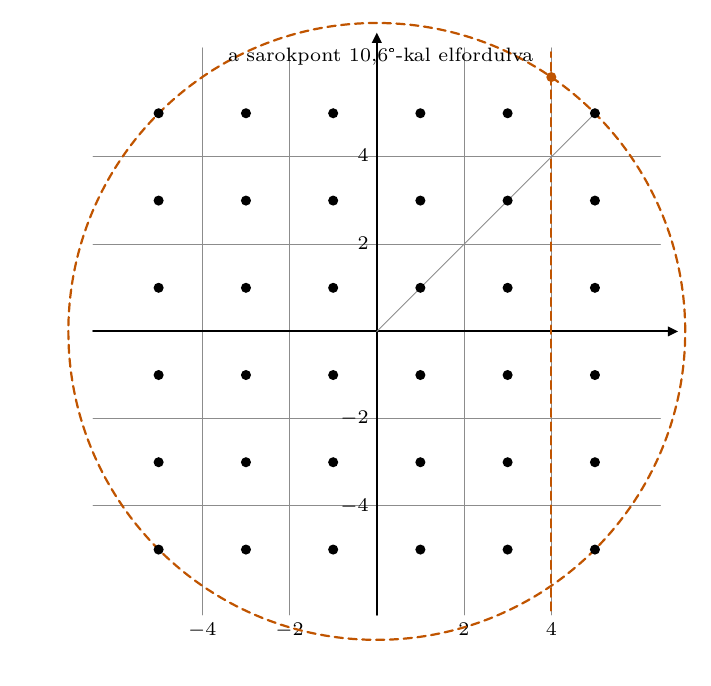
\begin{tikzpicture}[x=0.01600cm,y=-0.01600cm,line cap=round,line join=round]
\useasboundingbox (0,0) rectangle (520,500);
\path[draw=black!45,line width=0.35pt] (138.5,466) -- (138.5,16);
\path[draw=black!45,line width=0.35pt] (207.8,466) -- (207.8,16);
\path[draw=black!45,line width=0.35pt] (346.2,466) -- (346.2,16);
\path[draw=black!45,line width=0.35pt] (415.5,466) -- (415.5,16);
\path[draw=black!45,line width=0.35pt] (52,379.5) -- (502,379.5);
\path[draw=black!45,line width=0.35pt] (52,310.2) -- (502,310.2);
\path[draw=black!45,line width=0.35pt] (52,171.8) -- (502,171.8);
\path[draw=black!45,line width=0.35pt] (52,102.5) -- (502,102.5);
\path[draw=black,line width=0.7pt] (52,241) -- (510,241);
\path[fill=black,draw=none] (516,241) -- (508,237) -- (508,245) -- cycle;
\path[draw=black,line width=0.7pt] (277,466) -- (277,10);
\path[fill=black,draw=none] (277,4) -- (273,12) -- (281,12) -- cycle;
\node[anchor=base,inner sep=0pt,font=\scriptsize] at (138.5,482) {$-$4};
\node[anchor=base,inner sep=0pt,font=\scriptsize] at (207.8,482) {$-$2};
\node[anchor=base,inner sep=0pt,font=\scriptsize] at (346.2,482) {2};
\node[anchor=base,inner sep=0pt,font=\scriptsize] at (415.5,482) {4};
\node[anchor=base east,inner sep=0pt,font=\scriptsize] at (271,383.5) {$-$4};
\node[anchor=base east,inner sep=0pt,font=\scriptsize] at (271,314.2) {$-$2};
\node[anchor=base east,inner sep=0pt,font=\scriptsize] at (271,175.8) {2};
\node[anchor=base east,inner sep=0pt,font=\scriptsize] at (271,106.5) {4};
\path[draw=black!45,line width=0.35pt] (277,241) -- (450.1,67.9);
\path[draw=cB,line width=0.8pt,dash pattern=on 3pt off 2pt] (415.5,462.5) -- (415.5,19.5);
\path[draw=cB,line width=0.8pt,dash pattern=on 3pt off 2pt] (277,241) ellipse[x radius=3.917cm,y radius=3.917cm];
\path[fill=black,draw=none] (103.9,414.1) circle[radius=0.064cm];
\path[fill=black,draw=none] (103.9,344.8) circle[radius=0.064cm];
\path[fill=black,draw=none] (103.9,275.6) circle[radius=0.064cm];
\path[fill=black,draw=none] (103.9,206.4) circle[radius=0.064cm];
\path[fill=black,draw=none] (103.9,137.2) circle[radius=0.064cm];
\path[fill=black,draw=none] (103.9,67.9) circle[radius=0.064cm];
\path[fill=black,draw=none] (173.2,414.1) circle[radius=0.064cm];
\path[fill=black,draw=none] (173.2,344.8) circle[radius=0.064cm];
\path[fill=black,draw=none] (173.2,275.6) circle[radius=0.064cm];
\path[fill=black,draw=none] (173.2,206.4) circle[radius=0.064cm];
\path[fill=black,draw=none] (173.2,137.2) circle[radius=0.064cm];
\path[fill=black,draw=none] (173.2,67.9) circle[radius=0.064cm];
\path[fill=black,draw=none] (242.4,414.1) circle[radius=0.064cm];
\path[fill=black,draw=none] (242.4,344.8) circle[radius=0.064cm];
\path[fill=black,draw=none] (242.4,275.6) circle[radius=0.064cm];
\path[fill=black,draw=none] (242.4,206.4) circle[radius=0.064cm];
\path[fill=black,draw=none] (242.4,137.2) circle[radius=0.064cm];
\path[fill=black,draw=none] (242.4,67.9) circle[radius=0.064cm];
\path[fill=black,draw=none] (311.6,414.1) circle[radius=0.064cm];
\path[fill=black,draw=none] (311.6,344.8) circle[radius=0.064cm];
\path[fill=black,draw=none] (311.6,275.6) circle[radius=0.064cm];
\path[fill=black,draw=none] (311.6,206.4) circle[radius=0.064cm];
\path[fill=black,draw=none] (311.6,137.2) circle[radius=0.064cm];
\path[fill=black,draw=none] (311.6,67.9) circle[radius=0.064cm];
\path[fill=black,draw=none] (380.8,414.1) circle[radius=0.064cm];
\path[fill=black,draw=none] (380.8,344.8) circle[radius=0.064cm];
\path[fill=black,draw=none] (380.8,275.6) circle[radius=0.064cm];
\path[fill=black,draw=none] (380.8,206.4) circle[radius=0.064cm];
\path[fill=black,draw=none] (380.8,137.2) circle[radius=0.064cm];
\path[fill=black,draw=none] (380.8,67.9) circle[radius=0.064cm];
\path[fill=black,draw=none] (450.1,414.1) circle[radius=0.064cm];
\path[fill=black,draw=none] (450.1,344.8) circle[radius=0.064cm];
\path[fill=black,draw=none] (450.1,275.6) circle[radius=0.064cm];
\path[fill=black,draw=none] (450.1,206.4) circle[radius=0.064cm];
\path[fill=black,draw=none] (450.1,137.2) circle[radius=0.064cm];
\path[fill=black,draw=none] (450.1,67.9) circle[radius=0.064cm];
\path[fill=cB,draw=none] (415.5,39.2) circle[radius=0.064cm];
\node[anchor=base east,inner sep=0pt,font=\scriptsize] at (401.6,27) {a sarokpont 10,6\textdegree{}-kal elfordulva};
\end{tikzpicture}\end{center}
\begin{itemize}
\item $6\times6$ pont a $\pm1$, $\pm3$, $\pm5$ koordinátákon, a döntési határok (rács) a 0, $\pm2$, $\pm4$ értékeknél.
\item A sarokpont $(5,5)$ a legmesszebb van, $5\sqrt2$ sugarú körön mozog elforduláskor. 10,6\textdegree{}-nál éri el a 4-es határt (piros szaggatott).
\end{itemize}
\end{rajz}
\begin{tipp}[A gyűjtemény megoldása]
A gyűjtemény fázistűrése $\arcsin(1/5)=11{,}5^{\circ}$ (az $(5,1)$ pontra), d)-re „a fázishiba nem változik”, b)-re „pontosabban megállapíthatók a hibák”.
\end{tipp}
\begin{figyelem}[Javítás]
A szűk keresztmetszet a sarokpont (10,6\textdegree{}), nem az $(5,1)$ pont. A d) részben a fázistűrés 8,1\textdegree{}-ra romlik. A b) lényege a két csatorna független döntése. Nagyobb rácsnál van értelme az áthelyezésnek: a 64-QAM $(7,7)$ pontja $7\sqrt2=9{,}9$, a $(9,1)$ csak $\sqrt{82}=9{,}06$ távolságra van.
\end{figyelem}
\begin{eredmeny}

\begin{center}\adjustbox{max width=\linewidth}{$\displaystyle \text{c) }-20\%\ \text{és}\ +33\%,\ \varphi_{\max}=10{,}6^{\circ}\qquad\text{d) itt nincs előnye, a fázistűrés }8{,}1^{\circ}\text{-ra romlik}$}\end{center}
\end{eredmeny}


% ------------------------------------------------------------------
\section{\texorpdfstring{2.3. feladat: 16-PSK hibatűrése, 500 kbit/s sávigénye}{2.3. feladat: 16-PSK hibatűrése, 500 kbit/s sávigénye}}\label{o2_03}
\setcounter{lepes}{0}
\begin{feladat}{2.3. feladat}
a) A 16-PSK elméleti amplitúdó- és fázishibatűrése? Mi határolja a gyakorlatban az amplitúdótűrést? b) 500 kbit/s ISI-mentes átvitele legalább mekkora sávot kíván 16-PSK-val?

{\footnotesize\sffamily Forrás: 5-ösöm 8. oldal $\cdot$ 5o\_08\_1. Címkék: vizsga}
\end{feladat}
\begin{keresunk}
\begin{itemize}
\item a) amplitúdó- és fázistűrés
\item b) $B_{\min}$: a legkisebb sávszélesség
\end{itemize}
\end{keresunk}
\begin{jeloles}
\begin{jeltabla}
$\ca{M}$ & a konstelláció pontjainak száma & $16$\\
$\cb{v}$ & bitsebesség & $500$\,kbit/s\\
$B_{\min}$ & a legkisebb sávszélesség & \emph{keresett}\\
$\varphi_{\max}$ & a megengedett fázishiba & \\
$\alpha$ & lekerekítési tényező & \\
$B$ & a rendelkezésre álló sávszélesség & \\
$T$ & jelzési (bit-) idő & \\
$R_s$ & szimbólumsebesség & \\
\end{jeltabla}
\end{jeloles}

\lepes{a) Fázistűrés}
A 16 pont $360^{\circ}/{\ca{16}}=22{,}5^{\circ}$-onként van. A döntési határ két pont között félúton húzódik, így egy pont mindkét irányban a szögköz felével fordulhat el.

\begin{center}\adjustbox{max width=\linewidth}{$\displaystyle \varphi_{\max}=\frac{360^{\circ}}{16}\cdot\frac12=11{,}25^{\circ}$}\end{center}
\jegyzet{geometria}{}

\lepes{a) Amplitúdótűrés}
A PSK-ban minden pont ugyanazon a körön van, a döntés csak a szögtől függ. Az amplitúdó változása elméletben nem okoz hibát: a tűrés végtelen. A gyakorlatban a zaj határol: kis amplitúdónál ugyanaz a zaj nagyobb szögben forgatja el a pontot, így könnyebben átkerül a szomszéd szektorba.

\lepes{b) A legkisebb sáv}
Egy 16-PSK szimbólum $\log_216=4$ bitet visz. A legkisebb sáv $\alpha=0$-val adódik, vivőfrekvenciás átvitelnél $B=(1+\alpha)/T$ (A2).

\begin{center}\adjustbox{max width=\linewidth}{$\displaystyle R_s=\frac{v}{\log_2{\ca{M}}}=\frac{500}{4}=125\ \text{kBd}$}\end{center}
\jegyzet{számérték}{}

\begin{center}\adjustbox{max width=\linewidth}{$\displaystyle B_{\min}=\frac{1+0}{T}=R_s=125\ \text{kHz}$}\end{center}
\jegyzet{tétel}{$\alpha=0$}
\begin{eredmeny}

\begin{center}\adjustbox{max width=\linewidth}{$\displaystyle \text{a) amplitúdó: elméletben végtelen, fázis: }\pm11{,}25^{\circ}\qquad\text{b) }B_{\min}=125\ \text{kHz}$}\end{center}
\end{eredmeny}
\begin{tipp}[Ellenőrzés]
\begin{itemize}
\item A gyűjtemény „$\cdot$2?” kérdésére: vivőfrekvenciás átvitelnél nem kell kétszerezni, mert a $(1+\alpha)/T$ már a két oldalsávot tartalmazza. Alapsávban a fele, 62,5 kHz lenne.
\end{itemize}
\end{tipp}


% ------------------------------------------------------------------
\section{\texorpdfstring{2.4. feladat: 64-QAM kevesebb teljesítménnyel}{2.4. feladat: 64-QAM kevesebb teljesítménnyel}}\label{o2_04}
\setcounter{lepes}{0}
\begin{feladat}{2.4. feladat}
64-QAM-nél azonos hibaarány mellett csökkenteni kell a teljesítményt. Tippek?

{\footnotesize\sffamily Forrás: 5-ösöm 8. oldal $\cdot$ 5o\_08\_2. Címkék: beugró}
\end{feladat}
\begin{keresunk}
\begin{itemize}
\item ötletek a teljesítmény csökkentésére
\end{itemize}
\end{keresunk}
\begin{jeloles}
\begin{jeltabla}
$d$ & egy pont távolsága az origótól & \\
\end{jeltabla}
\par\smallskip\textbf{Adott még:}
\begin{itemize}
\item 64-QAM: $8\times8$-as rács, szintek $\pm1,\pm3,\pm5,\pm7$ tengelyenként
\item a hibaarányt (zajos csatornán) a pontok közti legkisebb távolság szabja meg, ez maradjon 2
\end{itemize}
\end{jeloles}

\lepes{Hol van a teljesítmény?}
Egy pont teljesítménye a távolsága négyzetével arányos. Az átlagos teljesítmény tengelyenként a négyzetek átlaga, a sarokpont ennek több mint kétszerese.

\begin{center}\adjustbox{max width=\linewidth}{$\displaystyle \overline{d^2}=2\cdot\frac{1+9+25+49}{4}=42$}\end{center}
\jegyzet{számérték}{a két tengely összesen}

\begin{center}\adjustbox{max width=\linewidth}{$\displaystyle d^2_\text{sarok}=7^2+7^2=98$}\end{center}
\jegyzet{számérték}{a (7,7) pont}

\lepes{1. ötlet: más alakú konstelláció}
A sarokpontokat beljebb, a tengelyek közelébe, üres rácshelyekre kell tenni, a legkisebb 2-es távolságot megtartva. Így kereszt alakú, ideálisan közel kör alakú elrendezés lesz: csökken az átlag- és a csúcsteljesítmény, a hibaarány nem változik.

\lepes{További ötletek}
Hibajavító kódolás (kódolási nyereség: ugyanakkora hibaarány kisebb jel-zaj viszonnyal), kisebb zajú vevő, nagyobb nyereségű antenna.
\begin{eredmeny}

\begin{center}\adjustbox{max width=\linewidth}{$\displaystyle \text{kör vagy kereszt alakú konstelláció azonos legkisebb távolsággal, illetve hibajavító kód}$}\end{center}
\end{eredmeny}
\begin{tipp}[Ellenőrzés]
\begin{itemize}
\item A gyűjteményben „64$\times$64-es mátrix” áll, helyesen 8$\times$8-as rács.
\end{itemize}
\end{tipp}


% ------------------------------------------------------------------
\section{\texorpdfstring{2.5. feladat: Tribites QAM a megfigyelt pontokkal}{2.5. feladat: Tribites QAM a megfigyelt pontokkal}}\label{o2_05}
\setcounter{lepes}{0}
\begin{feladat}{2.5. feladat}
Tribitek $(d_k,c_k)$: 000 (+1,+1), 001 (0,+3), 010 ($-$1,+1), 011 ($-$3,0), 100 ($-$1,$-$1), 101 (0,$-$3), 110 (+1,$-$1), 111 (+3,0). Megfigyelve: $(-0{,}20;\ 2{,}99)$, $(-0{,}94;\ -1{,}07)$, $(-1{,}08;\ 0{,}93)$, $(-2{,}98;\ -0{,}21)$. b) Tribitsorozat? c) Erősítéshiba? d) Fázishiba? e) Zaj?

{\footnotesize\sffamily Forrás: 5-ösöm 9. oldal $\cdot$ 5o\_09\_1 (gépelt megoldás). Címkék: vizsga, javítás}
\end{feladat}
\begin{keresunk}
\begin{itemize}
\item b) melyik tribitet küldték
\item c) erősítéshiba: a vett és az ideális távolság aránya
\item d) fázishiba: a vett és az ideális szög különbsége
\item e) a zaj nagysága
\end{itemize}
\end{keresunk}
\begin{jeloles}
\begin{jeltabla}
$d_k$ & a vízszintes koordináta & \\
$c_k$ & a függőleges koordináta & \\
$k$ & erősítési tényező & \\
$c$ & a vett pont függőleges koordinátája & \\
$d$ & a vett pont vízszintes koordinátája & \\
$\varphi$ & fázishiba & \\
\end{jeltabla}
\par\smallskip\textbf{Adott még:}
\begin{itemize}
\item a nyolc ideális pont $(d_k,c_k)$ koordinátái: $d_k$ a vízszintes, $c_k$ a függőleges tengely
\item négy vett (zajos, torzult) pont
\end{itemize}
\end{jeloles}

\lepes{b) A legközelebbi ideális pont}
Minden vett ponthoz megkeressük a legközelebbi ideális pontot (minimális távolságú döntés).

\begin{center}\adjustbox{max width=\linewidth}{$\displaystyle (-0{,}20;\ 2{,}99)\to(0,3)=001\qquad(-0{,}94;\ -1{,}07)\to(-1,-1)=100$}\end{center}
\jegyzet{számérték}{}

\begin{center}\adjustbox{max width=\linewidth}{$\displaystyle (-1{,}08;\ 0{,}93)\to(-1,1)=010\qquad(-2{,}98;\ -0{,}21)\to(-3,0)=011$}\end{center}
\jegyzet{számérték}{}

\lepes{c) Erősítéshiba}
A vett pont origótól mért távolságát osztjuk az ideáliséval.

\begin{center}\adjustbox{max width=\linewidth}{$\displaystyle \frac{\sqrt{0{,}20^2+2{,}99^2}}{3}=\frac{2{,}997}{3}=0{,}999\qquad\frac{\sqrt{0{,}94^2+1{,}07^2}}{\sqrt2}=\frac{1{,}424}{1{,}414}=1{,}007$}\end{center}
\jegyzet{geometria}{}

\begin{center}\adjustbox{max width=\linewidth}{$\displaystyle \frac{1{,}425}{1{,}414}=1{,}008\qquad\frac{2{,}987}{3}=0{,}996$}\end{center}
\jegyzet{geometria}{a harmadik és a negyedik pont}

\begin{center}\adjustbox{max width=\linewidth}{$\displaystyle k\approx1$}\end{center}
\jegyzet{számérték}{nincs számottevő erősítéshiba}

\lepes{d) Fázishiba}
A szöget az $\mathrm{atan2}(c,d)$ adja, ami a síknegyedet is helyesen kezeli. Az ideális szögekkel összevetve:

\begin{center}\adjustbox{max width=\linewidth}{$\displaystyle 93{,}8^{\circ}-90^{\circ}=3{,}8^{\circ}\qquad228{,}7^{\circ}-225^{\circ}=3{,}7^{\circ}$}\end{center}
\jegyzet{geometria}{1. és 2. pont}

\begin{center}\adjustbox{max width=\linewidth}{$\displaystyle 139{,}3^{\circ}-135^{\circ}=4{,}3^{\circ}\qquad184{,}0^{\circ}-180^{\circ}=4{,}0^{\circ}$}\end{center}
\jegyzet{geometria}{3. és 4. pont}

\begin{center}\adjustbox{max width=\linewidth}{$\displaystyle \varphi\approx4^{\circ}$}\end{center}
\jegyzet{számérték}{mind a négy ugyanannyit fordult}

\lepes{e) Zaj}
Ha zaj okozná az eltérést, a pontok véletlenszerűen, különböző irányba mozdulnának el. Itt mind a négy ugyanannyit fordult (3,7\textdegree{} és 4,3\textdegree{} között) és a távolságuk 1\%-on belül egyezik: a maradék szórás nagyon kicsi, a zaj elhanyagolható.

\begin{rajz}
\textbf{A nyolc tribit és a vett pontok}\par
\begin{center}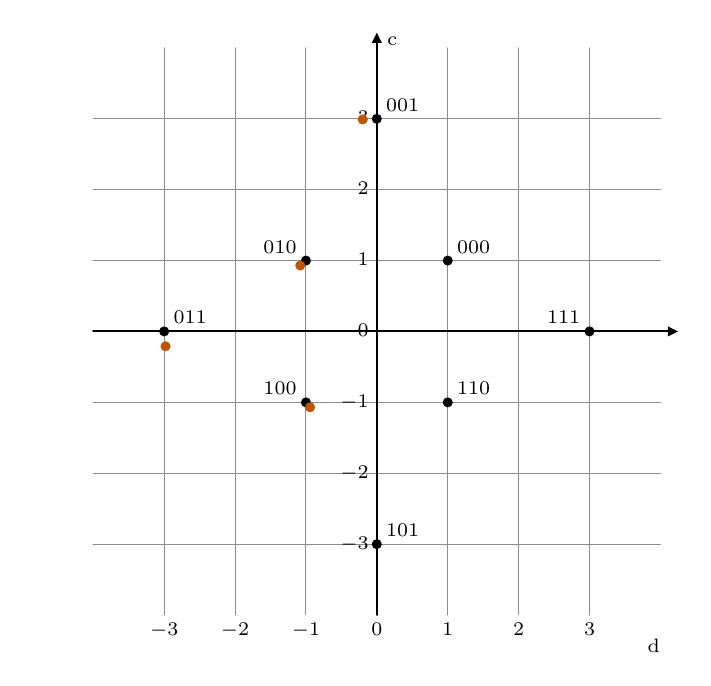
\begin{tikzpicture}[x=0.01600cm,y=-0.01600cm,line cap=round,line join=round]
\useasboundingbox (0,0) rectangle (520,500);
\path[draw=black!45,line width=0.35pt] (108.3,466) -- (108.3,16);
\path[draw=black!45,line width=0.35pt] (164.5,466) -- (164.5,16);
\path[draw=black!45,line width=0.35pt] (220.8,466) -- (220.8,16);
\path[draw=black!45,line width=0.35pt] (277,466) -- (277,16);
\path[draw=black!45,line width=0.35pt] (333.3,466) -- (333.3,16);
\path[draw=black!45,line width=0.35pt] (389.5,466) -- (389.5,16);
\path[draw=black!45,line width=0.35pt] (445.8,466) -- (445.8,16);
\path[draw=black!45,line width=0.35pt] (52,409.8) -- (502,409.8);
\path[draw=black!45,line width=0.35pt] (52,353.5) -- (502,353.5);
\path[draw=black!45,line width=0.35pt] (52,297.3) -- (502,297.3);
\path[draw=black!45,line width=0.35pt] (52,241) -- (502,241);
\path[draw=black!45,line width=0.35pt] (52,184.8) -- (502,184.8);
\path[draw=black!45,line width=0.35pt] (52,128.5) -- (502,128.5);
\path[draw=black!45,line width=0.35pt] (52,72.3) -- (502,72.3);
\path[draw=black,line width=0.7pt] (52,241) -- (510,241);
\path[fill=black,draw=none] (516,241) -- (508,237) -- (508,245) -- cycle;
\path[draw=black,line width=0.7pt] (277,466) -- (277,10);
\path[fill=black,draw=none] (277,4) -- (273,12) -- (281,12) -- cycle;
\node[anchor=base,inner sep=0pt,font=\scriptsize] at (108.3,482) {$-$3};
\node[anchor=base,inner sep=0pt,font=\scriptsize] at (164.5,482) {$-$2};
\node[anchor=base,inner sep=0pt,font=\scriptsize] at (220.8,482) {$-$1};
\node[anchor=base,inner sep=0pt,font=\scriptsize] at (277,482) {0};
\node[anchor=base,inner sep=0pt,font=\scriptsize] at (333.3,482) {1};
\node[anchor=base,inner sep=0pt,font=\scriptsize] at (389.5,482) {2};
\node[anchor=base,inner sep=0pt,font=\scriptsize] at (445.8,482) {3};
\node[anchor=base east,inner sep=0pt,font=\scriptsize] at (271,413.8) {$-$3};
\node[anchor=base east,inner sep=0pt,font=\scriptsize] at (271,357.5) {$-$2};
\node[anchor=base east,inner sep=0pt,font=\scriptsize] at (271,301.3) {$-$1};
\node[anchor=base east,inner sep=0pt,font=\scriptsize] at (271,245) {0};
\node[anchor=base east,inner sep=0pt,font=\scriptsize] at (271,188.8) {1};
\node[anchor=base east,inner sep=0pt,font=\scriptsize] at (271,132.5) {2};
\node[anchor=base east,inner sep=0pt,font=\scriptsize] at (271,76.3) {3};
\node[anchor=base east,inner sep=0pt,font=\scriptsize] at (502,496) {d};
\node[anchor=base west,inner sep=0pt,font=\scriptsize] at (285,14) {c};
\path[fill=black,draw=none] (333.3,184.8) circle[radius=0.064cm];
\node[anchor=base west,inner sep=0pt,font=\scriptsize] at (340.3,178.8) {000};
\path[fill=black,draw=none] (277,72.3) circle[radius=0.064cm];
\node[anchor=base west,inner sep=0pt,font=\scriptsize] at (284,66.3) {001};
\path[fill=black,draw=none] (220.8,184.8) circle[radius=0.064cm];
\node[anchor=base east,inner sep=0pt,font=\scriptsize] at (213.8,178.8) {010};
\path[fill=black,draw=none] (108.3,241) circle[radius=0.064cm];
\node[anchor=base west,inner sep=0pt,font=\scriptsize] at (115.3,235) {011};
\path[fill=black,draw=none] (220.8,297.3) circle[radius=0.064cm];
\node[anchor=base east,inner sep=0pt,font=\scriptsize] at (213.8,291.3) {100};
\path[fill=black,draw=none] (277,409.8) circle[radius=0.064cm];
\node[anchor=base west,inner sep=0pt,font=\scriptsize] at (284,403.8) {101};
\path[fill=black,draw=none] (333.3,297.3) circle[radius=0.064cm];
\node[anchor=base west,inner sep=0pt,font=\scriptsize] at (340.3,291.3) {110};
\path[fill=black,draw=none] (445.8,241) circle[radius=0.064cm];
\node[anchor=base east,inner sep=0pt,font=\scriptsize] at (438.8,235) {111};
\path[fill=cB,draw=none] (265.8,72.8) circle[radius=0.064cm];
\path[fill=cB,draw=none] (224.1,301.2) circle[radius=0.064cm];
\path[fill=cB,draw=none] (216.3,188.7) circle[radius=0.064cm];
\path[fill=cB,draw=none] (109.4,252.8) circle[radius=0.064cm];
\end{tikzpicture}\end{center}
\begin{itemize}
\item Kék pontok: az ideális tribitek. Piros pontok: a vett értékek, mind kb. 4\textdegree{}-kal az óramutatóval ellentétesen elfordulva, ugyanazon a sugáron.
\end{itemize}
\end{rajz}
\begin{tipp}[A gyűjtemény megoldása]
A gépelt megoldás szerint „a fázishiba nagy: $\tan^{-1}(-1{,}08/0{,}93)=130{,}73^{\circ}\ne145^{\circ}$”.
\end{tipp}
\begin{figyelem}[Javítás]
A gyűjtemény felcserélte a tengelyeket és rossz síknegyedet vett. Helyesen $\mathrm{atan2}(0{,}93;\,-1{,}08)=139{,}3^{\circ}$ a várt 135\textdegree{} helyett, a fázishiba kb. 4\textdegree{}.
\end{figyelem}
\begin{eredmeny}

\begin{center}\adjustbox{max width=\linewidth}{$\displaystyle \text{b) }001\ 100\ 010\ 011\qquad\text{c) }k\approx1\qquad\text{d) }\varphi\approx4^{\circ}\qquad\text{e) a zaj elhanyagolható}$}\end{center}
\end{eredmeny}

% Generálva: html/build_tex.js (o03.js). Kézzel ne szerkeszd, a forrás a html/data mappa.
\setcounter{chapter}{2}
\chapter{\texorpdfstring{Digitális alapsávi átvitel (PAM, ISI)}{Digitális alapsávi átvitel (PAM, ISI)}}\label{f3}
Elemi jelből szemábra, ISI és a többszintű rendszer próbája, valamint az emelt koszinuszos spektrum leolvasása.

\section{Alapok, egyszerűen}
\subsection{\texorpdfstring{A1. Jelölések és a minta képlete}{A1. Jelölések és a minta képlete}}\label{b3-jel}
\par\noindent{\small\renewcommand{\arraystretch}{1.25}\begin{tabularx}{\linewidth}{@{}>{\raggedright\arraybackslash}X>{\raggedright\arraybackslash}X@{}}\toprule
\textbf{Jel} & \textbf{Jelentés}\\\midrule
undefined & a undefined-adik szimbólum értéke (binárisnál undefined, négyszintűnél undefined)\\
undefined & elemi jel: egyetlen undefined szimbólum hatására a vevőben megjelenő jel\\
undefined & az elemi jel értéke a saját mintavételi pillanatában\\
undefined & az elemi jel értéke egy jelzési idővel később (ez lóg át a következő szimbólumba)\\
undefined & jelzési idő\\
undefined & az elemi jel spektruma\\
\bottomrule\end{tabularx}}\par

A PAM-jel az eltolt elemi jelek összege, $x(t)=\sum_kd_kh(t-kT)$. Ha a $k$-adik mintát a saját elemi jele $h_0$-nál, az előző szimbólumé $h_1$-nél metszi, akkor

\begin{center}\adjustbox{max width=\linewidth}{$\displaystyle x_k=h_0d_k+h_1d_{k-1}$}\end{center}

A második tag a \textbf{szimbólumközti áthallás (ISI)}. A döntés akkor hibátlan, ha a legrosszabb esetben is a jó oldalon marad a küszöbnek. $M$ szintnél a küszöbök a névleges szintek ($h_0d$) között félúton vannak.

\subsection{\texorpdfstring{A2. Nyquist-feltétel, emelt koszinusz}{A2. Nyquist-feltétel, emelt koszinusz}}\label{b3-nyq}
Az ISI akkor tűnik el, ha a spektrum $1/T$-nként eltolt másolatainak összege állandó. Az emelt koszinuszos spektrum ilyen: $f_1=(1-\alpha)/(2T)$-ig lapos, $f_2=(1+\alpha)/(2T)$-re nullára csökken, és a lecsengés a $1/(2T)$ pontra (ahol az érték a fele) pontszimmetrikus. Ebből $1/(2T)=(f_1+f_2)/2$ és $\alpha=(f_2-f_1)/(f_2+f_1)$.

% ------------------------------------------------------------------
\section{\texorpdfstring{3.1. feladat: Elemi jel 1,15 és 0,25}{3.1. feladat: Elemi jel 1,15 és 0,25}}\label{o3_01}
\setcounter{lepes}{0}
\begin{feladat}{3.1. feladat}
Bináris PAM, $h=1{,}15$ a $[0,T]$-n, $0{,}25$ a $[T,2T]$-n. a) PAM jel a \ldots{}0-1-1-0-0-1\ldots{} sorra. b) Van-e ISI, ha $t_0=3T/4$? c) Négyszintű szemábra ($-3,-1,+1,+3$), alkalmas-e?

{\footnotesize\sffamily Forrás: 5-ösöm 10. oldal $\cdot$ 5o\_10\_1. Címkék: vizsga}
\end{feladat}
\begin{keresunk}
\begin{itemize}
\item a) $x(t)$ (a PAM-jel) szintjei a bitsorra
\item b) van-e ISI, és okoz-e hibát
\item c) nyitott-e a négyszintű szem
\end{itemize}
\end{keresunk}
\begin{jeloles}
\begin{jeltabla}
$h$ & az elemi jel: 1,15 az első és 0,25 a második jelzési időben & \\
$T$ & jelzési idő & \\
$d_k$ & a k-adik szimbólum (+1 vagy $-$1) & \\
$\ca{t_0}$ & a mintavétel helye a jelzési időn belül & $3$\\
$x$ & a mintavevő kimenete (egy minta értéke) & \emph{keresett}\\
$k$ & az időrés sorszáma & \\
$x_k$ & a k-adik időrésben vett minta & \\
$d_{k-1}$ & az előző szimbólum (+1 vagy $-$1) & \\
$h_0$ & az elemi jel: 1,15 az első és 0,25 a második jelzési időben & \\
$h_1$ & az elemi jel: 1,15 az első és 0,25 a második jelzési időben & \\
$d$ & a szimbólum értéke, +1 az 1-es és $-$1 a 0-s bitre & \\
\end{jeltabla}
\end{jeloles}

\lepes{A minták képlete}
A $k$-adik időrésben ($kT$ és $(k+1)T$ között) a saját elemi jel első szakasza (1,15) és az előző szimbólum elemi jelének második szakasza (0,25) adódik össze. A $3T/4$-es mintavétel ebbe az időrésbe esik, így ez a minta is.

\begin{center}\adjustbox{max width=\linewidth}{$\displaystyle x_k=1{,}15\,d_k+0{,}25\,d_{k-1}$}\end{center}
\jegyzet{definíció}{$h_0=1{,}15$, $h_1=0{,}25$}

\lepes{a) A PAM-jel a bitsorra}
A bitsor $d=-1,+1,+1,-1,-1,+1$. Minden időrésre behelyettesítünk (az elsőhöz az előző bit nem ismert).

\begin{center}\adjustbox{max width=\linewidth}{$\displaystyle +1\text{ után }-1:\ 1{,}15-0{,}25=0{,}9\qquad+1\text{ után }+1:\ 1{,}15+0{,}25=1{,}4$}\end{center}
\jegyzet{behelyettesítés}{}

\begin{center}\adjustbox{max width=\linewidth}{$\displaystyle -1\text{ után }+1:\ -1{,}15+0{,}25=-0{,}9\qquad-1\text{ után }-1:\ -1{,}4$}\end{center}
\jegyzet{behelyettesítés}{}

\begin{center}\adjustbox{max width=\linewidth}{$\displaystyle x:\ -1{,}15\pm0{,}25,\ 0{,}9,\ 1{,}4,\ -0{,}9,\ -1{,}4,\ 0{,}9$}\end{center}
\jegyzet{számérték}{a hat időrés szintjei}

\lepes{b) ISI}
A minta értéke függ az előző bittől (0,9 vagy 1,4), tehát \textbf{van ISI}. Hibát viszont nem okoz: a döntési küszöb 0, és a legkisebb abszolút érték is $0{,}9>0$. A szem nyitott, a nyílása $2\cdot0{,}9=1{,}8$.

\lepes{c) Négyszintű rendszer}
Most $d_k\in\{-3,-1,1,3\}$, a névleges szintek $\pm1{,}15$ és $\pm3{,}45$, a küszöbök félúton: $0$ és $\pm2{,}3$. Az áthallás legfeljebb $0{,}25\cdot3=0{,}75$, mert $|d_{k-1}|\le3$.

\begin{center}\adjustbox{max width=\linewidth}{$\displaystyle d_k=1:\ 1{,}15-0{,}75=0{,}4>0\quad\text{és}\quad1{,}15+0{,}75=1{,}9<2{,}3$}\end{center}
\jegyzet{behelyettesítés}{a 0 és a 2,3 küszöb között marad}

\begin{center}\adjustbox{max width=\linewidth}{$\displaystyle d_k=3:\ 3{,}45-0{,}75=2{,}7>2{,}3$}\end{center}
\jegyzet{behelyettesítés}{a 2,3 felett marad}

\begin{center}\adjustbox{max width=\linewidth}{$\displaystyle 0{,}4>0$}\end{center}
\jegyzet{ellenőrzés}{a legrosszabb eset is a jó oldalon: alkalmas}

\begin{rajz}
\textbf{A PAM-jel a \ldots{}0-1-1-0-0-1\ldots{} bitsorra}\par
\begin{center}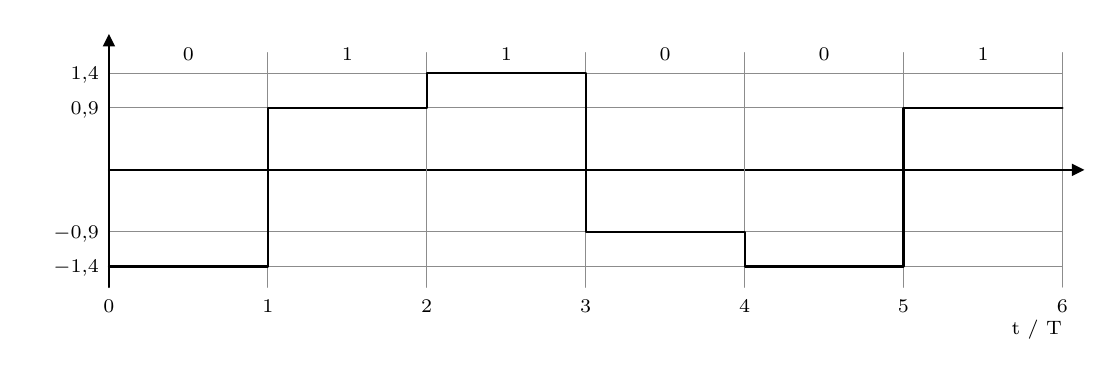
\begin{tikzpicture}[x=0.01985cm,y=-0.01985cm,line cap=round,line join=round]
\useasboundingbox (0,0) rectangle (680,200);
\path[draw=black!45,line width=0.35pt] (52,166) -- (52,16);
\path[draw=black!45,line width=0.35pt] (153.7,166) -- (153.7,16);
\path[draw=black!45,line width=0.35pt] (255.3,166) -- (255.3,16);
\path[draw=black!45,line width=0.35pt] (357,166) -- (357,16);
\path[draw=black!45,line width=0.35pt] (458.7,166) -- (458.7,16);
\path[draw=black!45,line width=0.35pt] (560.3,166) -- (560.3,16);
\path[draw=black!45,line width=0.35pt] (662,166) -- (662,16);
\path[draw=black!45,line width=0.35pt] (52,29.2) -- (662,29.2);
\path[draw=black!45,line width=0.35pt] (52,51.3) -- (662,51.3);
\path[draw=black!45,line width=0.35pt] (52,130.7) -- (662,130.7);
\path[draw=black!45,line width=0.35pt] (52,152.8) -- (662,152.8);
\path[draw=black,line width=0.7pt] (52,91) -- (670,91);
\path[fill=black,draw=none] (676,91) -- (668,87) -- (668,95) -- cycle;
\path[draw=black,line width=0.7pt] (52,166) -- (52,10);
\path[fill=black,draw=none] (52,4) -- (48,12) -- (56,12) -- cycle;
\node[anchor=base,inner sep=0pt,font=\scriptsize] at (52,182) {0};
\node[anchor=base,inner sep=0pt,font=\scriptsize] at (153.7,182) {1};
\node[anchor=base,inner sep=0pt,font=\scriptsize] at (255.3,182) {2};
\node[anchor=base,inner sep=0pt,font=\scriptsize] at (357,182) {3};
\node[anchor=base,inner sep=0pt,font=\scriptsize] at (458.7,182) {4};
\node[anchor=base,inner sep=0pt,font=\scriptsize] at (560.3,182) {5};
\node[anchor=base,inner sep=0pt,font=\scriptsize] at (662,182) {6};
\node[anchor=base east,inner sep=0pt,font=\scriptsize] at (46,33.2) {1,4};
\node[anchor=base east,inner sep=0pt,font=\scriptsize] at (46,55.3) {0,9};
\node[anchor=base east,inner sep=0pt,font=\scriptsize] at (46,134.7) {$-$0,9};
\node[anchor=base east,inner sep=0pt,font=\scriptsize] at (46,156.8) {$-$1,4};
\node[anchor=base east,inner sep=0pt,font=\scriptsize] at (662,196) {t / T};
\path[draw=black!45,line width=0.35pt,dash pattern=on 3pt off 2pt] (153.7,166) -- (153.7,16);
\path[draw=black!45,line width=0.35pt,dash pattern=on 3pt off 2pt] (255.3,166) -- (255.3,16);
\path[draw=black!45,line width=0.35pt,dash pattern=on 3pt off 2pt] (357,166) -- (357,16);
\path[draw=black!45,line width=0.35pt,dash pattern=on 3pt off 2pt] (458.7,166) -- (458.7,16);
\path[draw=black!45,line width=0.35pt,dash pattern=on 3pt off 2pt] (560.3,166) -- (560.3,16);
\path[draw=black,line width=0.8pt] (52,152.8) -- (153.7,152.8) -- (153.7,51.3) -- (255.3,51.3) -- (255.3,29.2) -- (357,29.2) -- (357,130.7) -- (458.7,130.7) -- (458.7,152.8) -- (560.3,152.8) -- (560.3,51.3) -- (662,51.3);
\node[anchor=base,inner sep=0pt,font=\scriptsize] at (102.8,21.3) {0};
\node[anchor=base,inner sep=0pt,font=\scriptsize] at (204.5,21.3) {1};
\node[anchor=base,inner sep=0pt,font=\scriptsize] at (306.2,21.3) {1};
\node[anchor=base,inner sep=0pt,font=\scriptsize] at (407.8,21.3) {0};
\node[anchor=base,inner sep=0pt,font=\scriptsize] at (509.5,21.3) {0};
\node[anchor=base,inner sep=0pt,font=\scriptsize] at (611.2,21.3) {1};
\end{tikzpicture}\end{center}
\begin{itemize}
\item Időrésenként egy vízszintes szakasz: $1{,}15\,d_k+0{,}25\,d_{k-1}$. Ha az előző bit ugyanaz, 1,4, ha más, 0,9 a szint (előjellel).
\item Az első időrésnél az előző bitet itt 0-nak ($-$1) vettük, ezért $-$1,4.
\end{itemize}

\textbf{Négyszintű szemábra a mintavételi pillanatban}\par
\begin{center}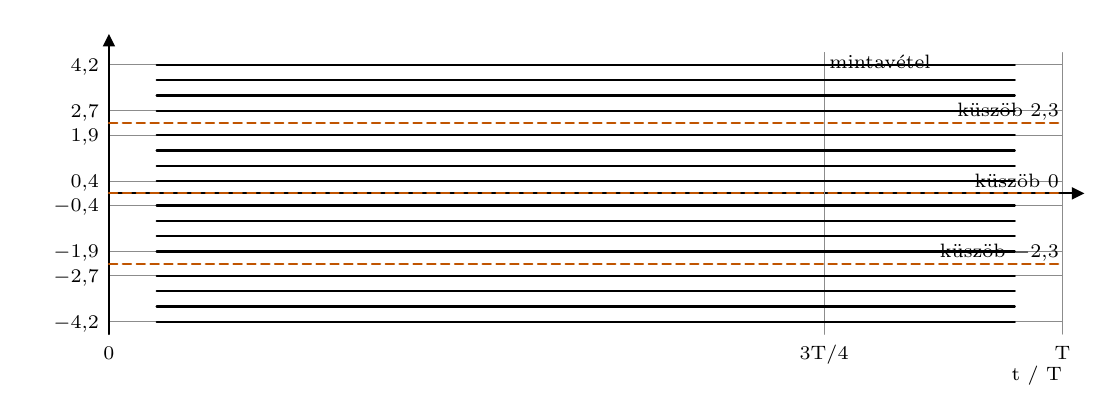
\begin{tikzpicture}[x=0.01985cm,y=-0.01985cm,line cap=round,line join=round]
\useasboundingbox (0,0) rectangle (680,230);
\path[draw=black!45,line width=0.35pt] (52,196) -- (52,16);
\path[draw=black!45,line width=0.35pt] (509.5,196) -- (509.5,16);
\path[draw=black!45,line width=0.35pt] (662,196) -- (662,16);
\path[draw=black!45,line width=0.35pt] (52,23.8) -- (662,23.8);
\path[draw=black!45,line width=0.35pt] (52,53.2) -- (662,53.2);
\path[draw=black!45,line width=0.35pt] (52,68.8) -- (662,68.8);
\path[draw=black!45,line width=0.35pt] (52,98.2) -- (662,98.2);
\path[draw=black!45,line width=0.35pt] (52,113.8) -- (662,113.8);
\path[draw=black!45,line width=0.35pt] (52,143.2) -- (662,143.2);
\path[draw=black!45,line width=0.35pt] (52,158.8) -- (662,158.8);
\path[draw=black!45,line width=0.35pt] (52,188.2) -- (662,188.2);
\path[draw=black,line width=0.7pt] (52,106) -- (670,106);
\path[fill=black,draw=none] (676,106) -- (668,102) -- (668,110) -- cycle;
\path[draw=black,line width=0.7pt] (52,196) -- (52,10);
\path[fill=black,draw=none] (52,4) -- (48,12) -- (56,12) -- cycle;
\node[anchor=base,inner sep=0pt,font=\scriptsize] at (52,212) {0};
\node[anchor=base,inner sep=0pt,font=\scriptsize] at (509.5,212) {3T/4};
\node[anchor=base,inner sep=0pt,font=\scriptsize] at (662,212) {T};
\node[anchor=base east,inner sep=0pt,font=\scriptsize] at (46,27.8) {4,2};
\node[anchor=base east,inner sep=0pt,font=\scriptsize] at (46,57.2) {2,7};
\node[anchor=base east,inner sep=0pt,font=\scriptsize] at (46,72.8) {1,9};
\node[anchor=base east,inner sep=0pt,font=\scriptsize] at (46,102.2) {0,4};
\node[anchor=base east,inner sep=0pt,font=\scriptsize] at (46,117.8) {$-$0,4};
\node[anchor=base east,inner sep=0pt,font=\scriptsize] at (46,147.2) {$-$1,9};
\node[anchor=base east,inner sep=0pt,font=\scriptsize] at (46,162.8) {$-$2,7};
\node[anchor=base east,inner sep=0pt,font=\scriptsize] at (46,192.2) {$-$4,2};
\node[anchor=base east,inner sep=0pt,font=\scriptsize] at (662,226) {t / T};
\path[draw=cB,line width=0.8pt,dash pattern=on 3pt off 2pt] (52,61) -- (662,61);
\node[anchor=base east,inner sep=0pt,font=\scriptsize] at (660,57) {küszöb 2,3};
\path[draw=cB,line width=0.8pt,dash pattern=on 3pt off 2pt] (52,106) -- (662,106);
\node[anchor=base east,inner sep=0pt,font=\scriptsize] at (660,102) {küszöb 0};
\path[draw=cB,line width=0.8pt,dash pattern=on 3pt off 2pt] (52,151) -- (662,151);
\node[anchor=base east,inner sep=0pt,font=\scriptsize] at (660,147) {küszöb $-$2,3};
\path[draw=black!45,line width=0.35pt,dash pattern=on 3pt off 2pt] (509.5,196) -- (509.5,16);
\node[anchor=base west,inner sep=0pt,font=\scriptsize] at (512.5,26) {mintavétel};
\path[draw=black,line width=0.8pt] (82.5,188.2) -- (631.5,188.2);
\path[draw=black,line width=0.8pt] (82.5,178.4) -- (631.5,178.4);
\path[draw=black,line width=0.8pt] (82.5,168.6) -- (631.5,168.6);
\path[draw=black,line width=0.8pt] (82.5,158.8) -- (631.5,158.8);
\path[draw=black,line width=0.8pt] (82.5,143.2) -- (631.5,143.2);
\path[draw=black,line width=0.8pt] (82.5,133.4) -- (631.5,133.4);
\path[draw=black,line width=0.8pt] (82.5,123.6) -- (631.5,123.6);
\path[draw=black,line width=0.8pt] (82.5,113.8) -- (631.5,113.8);
\path[draw=black,line width=0.8pt] (82.5,98.2) -- (631.5,98.2);
\path[draw=black,line width=0.8pt] (82.5,88.4) -- (631.5,88.4);
\path[draw=black,line width=0.8pt] (82.5,78.6) -- (631.5,78.6);
\path[draw=black,line width=0.8pt] (82.5,68.8) -- (631.5,68.8);
\path[draw=black,line width=0.8pt] (82.5,53.2) -- (631.5,53.2);
\path[draw=black,line width=0.8pt] (82.5,43.4) -- (631.5,43.4);
\path[draw=black,line width=0.8pt] (82.5,33.6) -- (631.5,33.6);
\path[draw=black,line width=0.8pt] (82.5,23.8) -- (631.5,23.8);
\end{tikzpicture}\end{center}
\begin{itemize}
\item Szimbólumonként négy vonal ($1{,}15d\pm0{,}25$ és $\pm0{,}75$): pl. $d=1$-nél 0,4, 0,9, 1,4, 1,9.
\item A szem nyitott: a 0,4 és a 2,7 is a saját küszöbe jó oldalán van. A legkisebb tartalék 0,4.
\end{itemize}
\end{rajz}
\begin{eredmeny}

\begin{center}\adjustbox{max width=\linewidth}{$\displaystyle \text{a) szintek }\pm0{,}9\text{ és }\pm1{,}4\qquad\text{b) van ISI, de hibát nem okoz}\qquad\text{c) igen, alkalmas (legkisebb tartalék 0,4)}$}\end{center}
\end{eredmeny}
\begin{tipp}[Ellenőrzés]
\begin{itemize}
\item A kézírás „1,15 $-$ 4$\cdot$0,25 $>$ 0”-t ír: a szorzó 3, mert a szomszéd szimbólum legfeljebb $\pm3$. A következtetés így is jó.
\end{itemize}
\end{tipp}


% ------------------------------------------------------------------
\section{\texorpdfstring{3.2. feladat: $\cos^2$ spektrumú elemi jel (hivatalos válasszal)}{3.2. feladat: cos2 spektrumú elemi jel (hivatalos válasszal)}}\label{o3_02}
\setcounter{lepes}{0}
\begin{feladat}{3.2. feladat}
$H(f)=h_0T\cos^2(\tfrac\pi2fT)$, ha $|f|<1/T$. a) Rajz. b) Elkerülhető-e az ISI? c) A szélessávú zajra optimális vevőszűrő? d) Okoz-e ISI-t egy 1200 Hz-es aluláteresztő, ha $T=833$ \textmu{}s?

{\footnotesize\sffamily Forrás: 5-ösöm 11. oldal $\cdot$ 5o\_11\_1. Címkék: vizsga}
\end{feladat}
\begin{keresunk}
\begin{itemize}
\item a) a spektrum alakja
\item b) teljesül-e a Nyquist-feltétel
\item c) $H_V(f)$: az optimális vevőszűrő
\item d) okoz-e ISI-t az 1200 Hz-es szűrő
\end{itemize}
\end{keresunk}
\begin{jeloles}
\begin{jeltabla}
$h_0$ & az elemi jel a saját mintavételi pillanatában & \\
$\ca{T}$ & jelzési idő & $833$\,\textmu{}s\\
$H_V$ & a vevőszűrő átvitele & \emph{keresett}\\
$x$ & tetszőleges szög (az azonosság változója) & \\
$\alpha$ & lekerekítési tényező & \\
$B_\text{jel}$ & a jel sávszélessége & \\
\end{jeltabla}
\end{jeloles}

\lepes{a) A spektrum alakja}
A $\cos^2x=\tfrac12(1+\cos2x)$ azonossággal emelt koszinusz alakra hozzuk.

\begin{center}\adjustbox{max width=\linewidth}{$\displaystyle H(f)=\frac{h_0{\ca{T}}}{2}\left(1+\cos\pi fT\right)$}\end{center}
\jegyzet{átalakítás}{}

\begin{center}\adjustbox{max width=\linewidth}{$\displaystyle H(0)=h_0{\ca{T}}\qquad H\!\left(\tfrac1{2{\ca{T}}}\right)=\tfrac{h_0{\ca{T}}}2\qquad H\!\left(\tfrac1{\ca{T}}\right)=0$}\end{center}
\jegyzet{számérték}{0-tól $1/T$-ig cseng le: 100\%-os emelt koszinusz, $\alpha=1$}

\lepes{b) Nyquist-feltétel}
Az ISI elkerülhető, ha a $1/{\ca{T}}$-nként eltolt másolatok összege állandó. A $0\le f\le1/{\ca{T}}$ tartományban két másolat fed át: $H(f)$ és $H(f-1/{\ca{T}})$.

\begin{center}\adjustbox{max width=\linewidth}{$\displaystyle \cos^2\!\left(\tfrac\pi2(f-\tfrac1{\ca{T}}){\ca{T}}\right)=\cos^2\!\left(\tfrac\pi2fT-\tfrac\pi2\right)=\sin^2\!\left(\tfrac\pi2fT\right)$}\end{center}
\jegyzet{átalakítás}{}

\begin{center}\adjustbox{max width=\linewidth}{$\displaystyle H(f)+H\!\left(f-\tfrac1{\ca{T}}\right)=h_0{\ca{T}}\left[\cos^2+\sin^2\right]=h_0{\ca{T}}$}\end{center}
\jegyzet{tétel}{állandó: ISI-mentes}

\lepes{c) Optimális vevőszűrő}
Fehér zajnál az optimális (illesztett) elrendezésben az adó- és a vevőszűrő egyformán osztozik a teljes $H(f)$-en, így a vevőszűrő $\sqrt{H}$-val arányos.

\begin{center}\adjustbox{max width=\linewidth}{$\displaystyle H_V(f)\propto\sqrt{H(f)}=\cos\left(\tfrac\pi2fT\right),\quad|f|<\tfrac1{\ca{T}}$}\end{center}
\jegyzet{definíció}{koszinusz félhullám}

\lepes{d) Az 1200 Hz-es szűrő}
A jel sávja $\alpha=1$ mellett $(1+\alpha)/(2{\ca{T}})=1/{\ca{T}}$.

\begin{center}\adjustbox{max width=\linewidth}{$\displaystyle \frac1{\ca{T}}=\frac{1}{833\ \mu\text{s}}=1200\ \text{Hz}$}\end{center}
\jegyzet{számérték}{}

\begin{center}\adjustbox{max width=\linewidth}{$\displaystyle B_\text{jel}=1200\ \text{Hz}\le1200\ \text{Hz}$}\end{center}
\jegyzet{ellenőrzés}{a szűrő a jel egyetlen összetevőjét sem vágja le}

\begin{rajz}
\textbf{A spektrum és eltolt másolata}\par
\begin{center}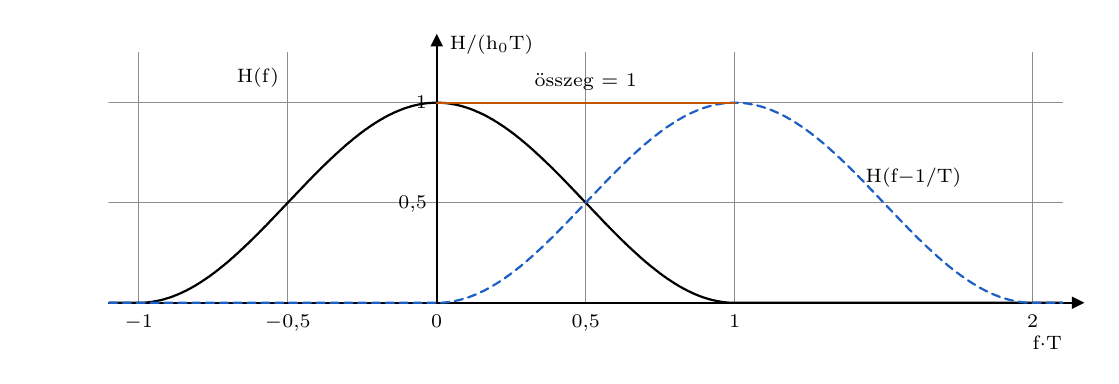
\begin{tikzpicture}[x=0.01985cm,y=-0.01985cm,line cap=round,line join=round]
\useasboundingbox (0,0) rectangle (680,210);
\path[draw=black!45,line width=0.35pt] (71.1,176) -- (71.1,16);
\path[draw=black!45,line width=0.35pt] (166.4,176) -- (166.4,16);
\path[draw=black!45,line width=0.35pt] (261.7,176) -- (261.7,16);
\path[draw=black!45,line width=0.35pt] (357,176) -- (357,16);
\path[draw=black!45,line width=0.35pt] (452.3,176) -- (452.3,16);
\path[draw=black!45,line width=0.35pt] (642.9,176) -- (642.9,16);
\path[draw=black!45,line width=0.35pt] (52,48) -- (662,48);
\path[draw=black!45,line width=0.35pt] (52,112) -- (662,112);
\path[draw=black,line width=0.7pt] (52,176) -- (670,176);
\path[fill=black,draw=none] (676,176) -- (668,172) -- (668,180) -- cycle;
\path[draw=black,line width=0.7pt] (261.7,176) -- (261.7,10);
\path[fill=black,draw=none] (261.7,4) -- (257.7,12) -- (265.7,12) -- cycle;
\node[anchor=base,inner sep=0pt,font=\scriptsize] at (71.1,192) {$-$1};
\node[anchor=base,inner sep=0pt,font=\scriptsize] at (166.4,192) {$-$0,5};
\node[anchor=base,inner sep=0pt,font=\scriptsize] at (261.7,192) {0};
\node[anchor=base,inner sep=0pt,font=\scriptsize] at (357,192) {0,5};
\node[anchor=base,inner sep=0pt,font=\scriptsize] at (452.3,192) {1};
\node[anchor=base,inner sep=0pt,font=\scriptsize] at (642.9,192) {2};
\node[anchor=base east,inner sep=0pt,font=\scriptsize] at (255.7,52) {1};
\node[anchor=base east,inner sep=0pt,font=\scriptsize] at (255.7,116) {0,5};
\node[anchor=base east,inner sep=0pt,font=\scriptsize] at (662,206) {f$\cdot$T};
\node[anchor=base west,inner sep=0pt,font=\scriptsize] at (269.7,14) {H/(h$_0$T)};
\path[draw=black,line width=0.8pt] (52,176) -- (52.8,176) -- (53.5,176) -- (54.3,176) -- (55.1,176) -- (55.8,176) -- (56.6,176) -- (57.3,176) -- (58.1,176) -- (58.9,176) -- (59.6,176) -- (60.4,176) -- (61.2,176) -- (61.9,176) -- (62.7,176) -- (63.4,176) -- (64.2,176) -- (65,176) -- (65.7,176) -- (66.5,176) -- (67.3,176) -- (68,176) -- (68.8,176) -- (69.5,176) -- (70.3,176) -- (71.1,176) -- (71.8,176) -- (72.6,176) -- (73.4,176) -- (74.1,175.9) -- (74.9,175.9) -- (75.6,175.8) -- (76.4,175.8) -- (77.2,175.7) -- (77.9,175.6) -- (78.7,175.5) -- (79.5,175.4) -- (80.2,175.3) -- (81,175.1) -- (81.7,175) -- (82.5,174.9) -- (83.3,174.7) -- (84,174.5) -- (84.8,174.4) -- (85.6,174.2) -- (86.3,174) -- (87.1,173.8) -- (87.8,173.6) -- (88.6,173.3) -- (89.4,173.1) -- (90.1,172.9) -- (90.9,172.6) -- (91.6,172.4) -- (92.4,172.1) -- (93.2,171.8) -- (93.9,171.5) -- (94.7,171.2) -- (95.5,170.9) -- (96.2,170.6) -- (97,170.2) -- (97.8,169.9) -- (98.5,169.6) -- (99.3,169.2) -- (100,168.8) -- (100.8,168.5) -- (101.6,168.1) -- (102.3,167.7) -- (103.1,167.3) -- (103.9,166.9) -- (104.6,166.5) -- (105.4,166) -- (106.1,165.6) -- (106.9,165.2) -- (107.7,164.7) -- (108.4,164.2) -- (109.2,163.8) -- (110,163.3) -- (110.7,162.8) -- (111.5,162.3) -- (112.2,161.8) -- (113,161.3) -- (113.8,160.8) -- (114.5,160.3) -- (115.3,159.7) -- (116.1,159.2) -- (116.8,158.7) -- (117.6,158.1) -- (118.3,157.5) -- (119.1,157) -- (119.9,156.4) -- (120.6,155.8) -- (121.4,155.2) -- (122.2,154.6) -- (122.9,154) -- (123.7,153.4) -- (124.4,152.8) -- (125.2,152.2) -- (126,151.5) -- (126.7,150.9) -- (127.5,150.3) -- (128.3,149.6) -- (129,149) -- (129.8,148.3) -- (130.5,147.6) -- (131.3,147) -- (132.1,146.3) -- (132.8,145.6) -- (133.6,144.9) -- (134.4,144.2) -- (135.1,143.5) -- (135.9,142.8) -- (136.6,142.1) -- (137.4,141.4) -- (138.2,140.7) -- (138.9,140) -- (139.7,139.2) -- (140.5,138.5) -- (141.2,137.8) -- (142,137) -- (142.7,136.3) -- (143.5,135.6) -- (144.3,134.8) -- (145,134.1) -- (145.8,133.3) -- (146.6,132.5) -- (147.3,131.8) -- (148.1,131) -- (148.8,130.2) -- (149.6,129.5) -- (150.4,128.7) -- (151.1,127.9) -- (151.9,127.1) -- (152.7,126.4) -- (153.4,125.6) -- (154.2,124.8) -- (154.9,124) -- (155.7,123.2) -- (156.5,122.4) -- (157.2,121.6) -- (158,120.8) -- (158.8,120) -- (159.5,119.2) -- (160.3,118.4) -- (161,117.6) -- (161.8,116.8) -- (162.6,116) -- (163.3,115.2) -- (164.1,114.4) -- (164.9,113.6) -- (165.6,112.8) -- (166.4,112) -- (167.1,111.2) -- (167.9,110.4) -- (168.7,109.6) -- (169.4,108.8) -- (170.2,108) -- (171,107.2) -- (171.7,106.4) -- (172.5,105.6) -- (173.2,104.8) -- (174,104) -- (174.8,103.2) -- (175.5,102.4) -- (176.3,101.6) -- (177.1,100.8) -- (177.8,100) -- (178.6,99.2) -- (179.3,98.4) -- (180.1,97.6) -- (180.9,96.9) -- (181.6,96.1) -- (182.4,95.3) -- (183.1,94.5) -- (183.9,93.8) -- (184.7,93) -- (185.4,92.2) -- (186.2,91.5) -- (187,90.7) -- (187.7,89.9) -- (188.5,89.2) -- (189.3,88.4) -- (190,87.7) -- (190.8,87) -- (191.5,86.2) -- (192.3,85.5) -- (193.1,84.8) -- (193.8,84) -- (194.6,83.3) -- (195.4,82.6) -- (196.1,81.9) -- (196.9,81.2) -- (197.6,80.5) -- (198.4,79.8) -- (199.2,79.1) -- (199.9,78.4) -- (200.7,77.7) -- (201.5,77) -- (202.2,76.4) -- (203,75.7) -- (203.7,75) -- (204.5,74.4) -- (205.3,73.7) -- (206,73.1) -- (206.8,72.5) -- (207.6,71.8) -- (208.3,71.2) -- (209.1,70.6) -- (209.8,70) -- (210.6,69.4) -- (211.4,68.8) -- (212.1,68.2) -- (212.9,67.6) -- (213.7,67) -- (214.4,66.5) -- (215.2,65.9) -- (215.9,65.3) -- (216.7,64.8) -- (217.5,64.3) -- (218.2,63.7) -- (219,63.2) -- (219.7,62.7) -- (220.5,62.2) -- (221.3,61.7) -- (222,61.2) -- (222.8,60.7) -- (223.6,60.2) -- (224.3,59.8) -- (225.1,59.3) -- (225.9,58.8) -- (226.6,58.4) -- (227.4,58) -- (228.1,57.5) -- (228.9,57.1) -- (229.7,56.7) -- (230.4,56.3) -- (231.2,55.9) -- (232,55.5) -- (232.7,55.2) -- (233.5,54.8) -- (234.2,54.4) -- (235,54.1) -- (235.8,53.8) -- (236.5,53.4) -- (237.3,53.1) -- (238.1,52.8) -- (238.8,52.5) -- (239.6,52.2) -- (240.3,51.9) -- (241.1,51.6) -- (241.9,51.4) -- (242.6,51.1) -- (243.4,50.9) -- (244.2,50.7) -- (244.9,50.4) -- (245.7,50.2) -- (246.4,50) -- (247.2,49.8) -- (248,49.6) -- (248.7,49.5) -- (249.5,49.3) -- (250.3,49.1) -- (251,49) -- (251.8,48.9) -- (252.5,48.7) -- (253.3,48.6) -- (254.1,48.5) -- (254.8,48.4) -- (255.6,48.3) -- (256.4,48.2) -- (257.1,48.2) -- (257.9,48.1) -- (258.6,48.1) -- (259.4,48) -- (260.2,48) -- (260.9,48) -- (261.7,48) -- (262.5,48) -- (263.2,48) -- (264,48) -- (264.7,48.1) -- (265.5,48.1) -- (266.3,48.2) -- (267,48.2) -- (267.8,48.3) -- (268.6,48.4) -- (269.3,48.5) -- (270.1,48.6) -- (270.8,48.7) -- (271.6,48.9) -- (272.4,49) -- (273.1,49.1) -- (273.9,49.3) -- (274.7,49.5) -- (275.4,49.6) -- (276.2,49.8) -- (276.9,50) -- (277.7,50.2) -- (278.5,50.4) -- (279.2,50.7) -- (280,50.9) -- (280.8,51.1) -- (281.5,51.4) -- (282.3,51.6) -- (283,51.9) -- (283.8,52.2) -- (284.6,52.5) -- (285.3,52.8) -- (286.1,53.1) -- (286.8,53.4) -- (287.6,53.8) -- (288.4,54.1) -- (289.1,54.4) -- (289.9,54.8) -- (290.7,55.2) -- (291.4,55.5) -- (292.2,55.9) -- (293,56.3) -- (293.7,56.7) -- (294.5,57.1) -- (295.2,57.5) -- (296,58) -- (296.8,58.4) -- (297.5,58.8) -- (298.3,59.3) -- (299,59.8) -- (299.8,60.2) -- (300.6,60.7) -- (301.3,61.2) -- (302.1,61.7) -- (302.9,62.2) -- (303.6,62.7) -- (304.4,63.2) -- (305.2,63.7) -- (305.9,64.3) -- (306.7,64.8) -- (307.4,65.3) -- (308.2,65.9) -- (309,66.5) -- (309.7,67) -- (310.5,67.6) -- (311.3,68.2) -- (312,68.8) -- (312.8,69.4) -- (313.5,70) -- (314.3,70.6) -- (315.1,71.2) -- (315.8,71.8) -- (316.6,72.5) -- (317.4,73.1) -- (318.1,73.7) -- (318.9,74.4) -- (319.6,75) -- (320.4,75.7) -- (321.2,76.4) -- (321.9,77) -- (322.7,77.7) -- (323.5,78.4) -- (324.2,79.1) -- (325,79.8) -- (325.7,80.5) -- (326.5,81.2) -- (327.3,81.9) -- (328,82.6) -- (328.8,83.3) -- (329.5,84) -- (330.3,84.8) -- (331.1,85.5) -- (331.8,86.2) -- (332.6,87) -- (333.4,87.7) -- (334.1,88.4) -- (334.9,89.2) -- (335.7,89.9) -- (336.4,90.7) -- (337.2,91.5) -- (337.9,92.2) -- (338.7,93) -- (339.5,93.8) -- (340.2,94.5) -- (341,95.3) -- (341.8,96.1) -- (342.5,96.9) -- (343.3,97.6) -- (344,98.4) -- (344.8,99.2) -- (345.6,100) -- (346.3,100.8) -- (347.1,101.6) -- (347.9,102.4) -- (348.6,103.2) -- (349.4,104) -- (350.1,104.8) -- (350.9,105.6) -- (351.7,106.4) -- (352.4,107.2) -- (353.2,108) -- (354,108.8) -- (354.7,109.6) -- (355.5,110.4) -- (356.2,111.2) -- (357,112) -- (357.8,112.8) -- (358.5,113.6) -- (359.3,114.4) -- (360.1,115.2) -- (360.8,116) -- (361.6,116.8) -- (362.3,117.6) -- (363.1,118.4) -- (363.9,119.2) -- (364.6,120) -- (365.4,120.8) -- (366.2,121.6) -- (366.9,122.4) -- (367.7,123.2) -- (368.4,124) -- (369.2,124.8) -- (370,125.6) -- (370.7,126.4) -- (371.5,127.1) -- (372.2,127.9) -- (373,128.7) -- (373.8,129.5) -- (374.5,130.2) -- (375.3,131) -- (376.1,131.8) -- (376.8,132.5) -- (377.6,133.3) -- (378.4,134.1) -- (379.1,134.8) -- (379.9,135.6) -- (380.6,136.3) -- (381.4,137) -- (382.2,137.8) -- (382.9,138.5) -- (383.7,139.2) -- (384.4,140) -- (385.2,140.7) -- (386,141.4) -- (386.7,142.1) -- (387.5,142.8) -- (388.3,143.5) -- (389,144.2) -- (389.8,144.9) -- (390.6,145.6) -- (391.3,146.3) -- (392.1,147) -- (392.8,147.6) -- (393.6,148.3) -- (394.4,149) -- (395.1,149.6) -- (395.9,150.3) -- (396.7,150.9) -- (397.4,151.5) -- (398.2,152.2) -- (398.9,152.8) -- (399.7,153.4) -- (400.5,154) -- (401.2,154.6) -- (402,155.2) -- (402.8,155.8) -- (403.5,156.4) -- (404.3,157) -- (405,157.5) -- (405.8,158.1) -- (406.6,158.7) -- (407.3,159.2) -- (408.1,159.7) -- (408.8,160.3) -- (409.6,160.8) -- (410.4,161.3) -- (411.1,161.8) -- (411.9,162.3) -- (412.7,162.8) -- (413.4,163.3) -- (414.2,163.8) -- (415,164.2) -- (415.7,164.7) -- (416.5,165.2) -- (417.2,165.6) -- (418,166) -- (418.8,166.5) -- (419.5,166.9) -- (420.3,167.3) -- (421.1,167.7) -- (421.8,168.1) -- (422.6,168.5) -- (423.3,168.8) -- (424.1,169.2) -- (424.9,169.6) -- (425.6,169.9) -- (426.4,170.2) -- (427.2,170.6) -- (427.9,170.9) -- (428.7,171.2) -- (429.4,171.5) -- (430.2,171.8) -- (431,172.1) -- (431.7,172.4) -- (432.5,172.6) -- (433.3,172.9) -- (434,173.1) -- (434.8,173.3) -- (435.5,173.6) -- (436.3,173.8) -- (437.1,174) -- (437.8,174.2) -- (438.6,174.4) -- (439.4,174.5) -- (440.1,174.7) -- (440.9,174.9) -- (441.6,175) -- (442.4,175.1) -- (443.2,175.3) -- (443.9,175.4) -- (444.7,175.5) -- (445.5,175.6) -- (446.2,175.7) -- (447,175.8) -- (447.7,175.8) -- (448.5,175.9) -- (449.3,175.9) -- (450,176) -- (450.8,176) -- (451.6,176) -- (452.3,176) -- (453.1,176) -- (453.8,176) -- (454.6,176) -- (455.4,176) -- (456.1,176) -- (456.9,176) -- (457.7,176) -- (458.4,176) -- (459.2,176) -- (459.9,176) -- (460.7,176) -- (461.5,176) -- (462.2,176) -- (463,176) -- (463.8,176) -- (464.5,176) -- (465.3,176) -- (466,176) -- (466.8,176) -- (467.6,176) -- (468.3,176) -- (469.1,176) -- (469.9,176) -- (470.6,176) -- (471.4,176) -- (472.1,176) -- (472.9,176) -- (473.7,176) -- (474.4,176) -- (475.2,176) -- (476,176) -- (476.7,176) -- (477.5,176) -- (478.2,176) -- (479,176) -- (479.8,176) -- (480.5,176) -- (481.3,176) -- (482.1,176) -- (482.8,176) -- (483.6,176) -- (484.3,176) -- (485.1,176) -- (485.9,176) -- (486.6,176) -- (487.4,176) -- (488.2,176) -- (488.9,176) -- (489.7,176) -- (490.4,176) -- (491.2,176) -- (492,176) -- (492.7,176) -- (493.5,176) -- (494.2,176) -- (495,176) -- (495.8,176) -- (496.5,176) -- (497.3,176) -- (498.1,176) -- (498.8,176) -- (499.6,176) -- (500.4,176) -- (501.1,176) -- (501.9,176) -- (502.6,176) -- (503.4,176) -- (504.2,176) -- (504.9,176) -- (505.7,176) -- (506.4,176) -- (507.2,176) -- (508,176) -- (508.7,176) -- (509.5,176) -- (510.3,176) -- (511,176) -- (511.8,176) -- (512.6,176) -- (513.3,176) -- (514.1,176) -- (514.8,176) -- (515.6,176) -- (516.4,176) -- (517.1,176) -- (517.9,176) -- (518.6,176) -- (519.4,176) -- (520.2,176) -- (520.9,176) -- (521.7,176) -- (522.5,176) -- (523.2,176) -- (524,176) -- (524.8,176) -- (525.5,176) -- (526.3,176) -- (527,176) -- (527.8,176) -- (528.6,176) -- (529.3,176) -- (530.1,176) -- (530.8,176) -- (531.6,176) -- (532.4,176) -- (533.1,176) -- (533.9,176) -- (534.7,176) -- (535.4,176) -- (536.2,176) -- (536.9,176) -- (537.7,176) -- (538.5,176) -- (539.2,176) -- (540,176) -- (540.8,176) -- (541.5,176) -- (542.3,176) -- (543.1,176) -- (543.8,176) -- (544.6,176) -- (545.3,176) -- (546.1,176) -- (546.9,176) -- (547.6,176) -- (548.4,176) -- (549.2,176) -- (549.9,176) -- (550.7,176) -- (551.4,176) -- (552.2,176) -- (553,176) -- (553.7,176) -- (554.5,176) -- (555.3,176) -- (556,176) -- (556.8,176) -- (557.5,176) -- (558.3,176) -- (559.1,176) -- (559.8,176) -- (560.6,176) -- (561.3,176) -- (562.1,176) -- (562.9,176) -- (563.6,176) -- (564.4,176) -- (565.2,176) -- (565.9,176) -- (566.7,176) -- (567.4,176) -- (568.2,176) -- (569,176) -- (569.7,176) -- (570.5,176) -- (571.3,176) -- (572,176) -- (572.8,176) -- (573.6,176) -- (574.3,176) -- (575.1,176) -- (575.8,176) -- (576.6,176) -- (577.4,176) -- (578.1,176) -- (578.9,176) -- (579.7,176) -- (580.4,176) -- (581.2,176) -- (581.9,176) -- (582.7,176) -- (583.5,176) -- (584.2,176) -- (585,176) -- (585.7,176) -- (586.5,176) -- (587.3,176) -- (588,176) -- (588.8,176) -- (589.6,176) -- (590.3,176) -- (591.1,176) -- (591.8,176) -- (592.6,176) -- (593.4,176) -- (594.1,176) -- (594.9,176) -- (595.7,176) -- (596.4,176) -- (597.2,176) -- (598,176) -- (598.7,176) -- (599.5,176) -- (600.2,176) -- (601,176) -- (601.8,176) -- (602.5,176) -- (603.3,176) -- (604.1,176) -- (604.8,176) -- (605.6,176) -- (606.3,176) -- (607.1,176) -- (607.9,176) -- (608.6,176) -- (609.4,176) -- (610.2,176) -- (610.9,176) -- (611.7,176) -- (612.4,176) -- (613.2,176) -- (614,176) -- (614.7,176) -- (615.5,176) -- (616.3,176) -- (617,176) -- (617.8,176) -- (618.5,176) -- (619.3,176) -- (620.1,176) -- (620.8,176) -- (621.6,176) -- (622.3,176) -- (623.1,176) -- (623.9,176) -- (624.6,176) -- (625.4,176) -- (626.2,176) -- (626.9,176) -- (627.7,176) -- (628.5,176) -- (629.2,176) -- (630,176) -- (630.7,176) -- (631.5,176) -- (632.3,176) -- (633,176) -- (633.8,176) -- (634.6,176) -- (635.3,176) -- (636.1,176) -- (636.8,176) -- (637.6,176) -- (638.4,176) -- (639.1,176) -- (639.9,176) -- (640.7,176) -- (641.4,176) -- (642.2,176) -- (642.9,176) -- (643.7,176) -- (644.5,176) -- (645.2,176) -- (646,176) -- (646.8,176) -- (647.5,176) -- (648.3,176) -- (649,176) -- (649.8,176) -- (650.6,176) -- (651.3,176) -- (652.1,176) -- (652.9,176) -- (653.6,176) -- (654.4,176) -- (655.1,176) -- (655.9,176) -- (656.7,176) -- (657.4,176) -- (658.2,176) -- (659,176) -- (659.7,176) -- (660.5,176) -- (661.2,176) -- (662,176);
\path[draw=cA,line width=0.8pt,dash pattern=on 3pt off 2pt] (52,176) -- (52.8,176) -- (53.5,176) -- (54.3,176) -- (55.1,176) -- (55.8,176) -- (56.6,176) -- (57.3,176) -- (58.1,176) -- (58.9,176) -- (59.6,176) -- (60.4,176) -- (61.2,176) -- (61.9,176) -- (62.7,176) -- (63.4,176) -- (64.2,176) -- (65,176) -- (65.7,176) -- (66.5,176) -- (67.3,176) -- (68,176) -- (68.8,176) -- (69.5,176) -- (70.3,176) -- (71.1,176) -- (71.8,176) -- (72.6,176) -- (73.4,176) -- (74.1,176) -- (74.9,176) -- (75.6,176) -- (76.4,176) -- (77.2,176) -- (77.9,176) -- (78.7,176) -- (79.5,176) -- (80.2,176) -- (81,176) -- (81.7,176) -- (82.5,176) -- (83.3,176) -- (84,176) -- (84.8,176) -- (85.6,176) -- (86.3,176) -- (87.1,176) -- (87.8,176) -- (88.6,176) -- (89.4,176) -- (90.1,176) -- (90.9,176) -- (91.6,176) -- (92.4,176) -- (93.2,176) -- (93.9,176) -- (94.7,176) -- (95.5,176) -- (96.2,176) -- (97,176) -- (97.8,176) -- (98.5,176) -- (99.3,176) -- (100,176) -- (100.8,176) -- (101.6,176) -- (102.3,176) -- (103.1,176) -- (103.9,176) -- (104.6,176) -- (105.4,176) -- (106.1,176) -- (106.9,176) -- (107.7,176) -- (108.4,176) -- (109.2,176) -- (110,176) -- (110.7,176) -- (111.5,176) -- (112.2,176) -- (113,176) -- (113.8,176) -- (114.5,176) -- (115.3,176) -- (116.1,176) -- (116.8,176) -- (117.6,176) -- (118.3,176) -- (119.1,176) -- (119.9,176) -- (120.6,176) -- (121.4,176) -- (122.2,176) -- (122.9,176) -- (123.7,176) -- (124.4,176) -- (125.2,176) -- (126,176) -- (126.7,176) -- (127.5,176) -- (128.3,176) -- (129,176) -- (129.8,176) -- (130.5,176) -- (131.3,176) -- (132.1,176) -- (132.8,176) -- (133.6,176) -- (134.4,176) -- (135.1,176) -- (135.9,176) -- (136.6,176) -- (137.4,176) -- (138.2,176) -- (138.9,176) -- (139.7,176) -- (140.5,176) -- (141.2,176) -- (142,176) -- (142.7,176) -- (143.5,176) -- (144.3,176) -- (145,176) -- (145.8,176) -- (146.6,176) -- (147.3,176) -- (148.1,176) -- (148.8,176) -- (149.6,176) -- (150.4,176) -- (151.1,176) -- (151.9,176) -- (152.7,176) -- (153.4,176) -- (154.2,176) -- (154.9,176) -- (155.7,176) -- (156.5,176) -- (157.2,176) -- (158,176) -- (158.8,176) -- (159.5,176) -- (160.3,176) -- (161,176) -- (161.8,176) -- (162.6,176) -- (163.3,176) -- (164.1,176) -- (164.9,176) -- (165.6,176) -- (166.4,176) -- (167.1,176) -- (167.9,176) -- (168.7,176) -- (169.4,176) -- (170.2,176) -- (171,176) -- (171.7,176) -- (172.5,176) -- (173.2,176) -- (174,176) -- (174.8,176) -- (175.5,176) -- (176.3,176) -- (177.1,176) -- (177.8,176) -- (178.6,176) -- (179.3,176) -- (180.1,176) -- (180.9,176) -- (181.6,176) -- (182.4,176) -- (183.1,176) -- (183.9,176) -- (184.7,176) -- (185.4,176) -- (186.2,176) -- (187,176) -- (187.7,176) -- (188.5,176) -- (189.3,176) -- (190,176) -- (190.8,176) -- (191.5,176) -- (192.3,176) -- (193.1,176) -- (193.8,176) -- (194.6,176) -- (195.4,176) -- (196.1,176) -- (196.9,176) -- (197.6,176) -- (198.4,176) -- (199.2,176) -- (199.9,176) -- (200.7,176) -- (201.5,176) -- (202.2,176) -- (203,176) -- (203.7,176) -- (204.5,176) -- (205.3,176) -- (206,176) -- (206.8,176) -- (207.6,176) -- (208.3,176) -- (209.1,176) -- (209.8,176) -- (210.6,176) -- (211.4,176) -- (212.1,176) -- (212.9,176) -- (213.7,176) -- (214.4,176) -- (215.2,176) -- (215.9,176) -- (216.7,176) -- (217.5,176) -- (218.2,176) -- (219,176) -- (219.7,176) -- (220.5,176) -- (221.3,176) -- (222,176) -- (222.8,176) -- (223.6,176) -- (224.3,176) -- (225.1,176) -- (225.9,176) -- (226.6,176) -- (227.4,176) -- (228.1,176) -- (228.9,176) -- (229.7,176) -- (230.4,176) -- (231.2,176) -- (232,176) -- (232.7,176) -- (233.5,176) -- (234.2,176) -- (235,176) -- (235.8,176) -- (236.5,176) -- (237.3,176) -- (238.1,176) -- (238.8,176) -- (239.6,176) -- (240.3,176) -- (241.1,176) -- (241.9,176) -- (242.6,176) -- (243.4,176) -- (244.2,176) -- (244.9,176) -- (245.7,176) -- (246.4,176) -- (247.2,176) -- (248,176) -- (248.7,176) -- (249.5,176) -- (250.3,176) -- (251,176) -- (251.8,176) -- (252.5,176) -- (253.3,176) -- (254.1,176) -- (254.8,176) -- (255.6,176) -- (256.4,176) -- (257.1,176) -- (257.9,176) -- (258.6,176) -- (259.4,176) -- (260.2,176) -- (260.9,176) -- (261.7,176) -- (262.5,176) -- (263.2,176) -- (264,176) -- (264.7,175.9) -- (265.5,175.9) -- (266.3,175.8) -- (267,175.8) -- (267.8,175.7) -- (268.6,175.6) -- (269.3,175.5) -- (270.1,175.4) -- (270.8,175.3) -- (271.6,175.1) -- (272.4,175) -- (273.1,174.9) -- (273.9,174.7) -- (274.7,174.5) -- (275.4,174.4) -- (276.2,174.2) -- (276.9,174) -- (277.7,173.8) -- (278.5,173.6) -- (279.2,173.3) -- (280,173.1) -- (280.8,172.9) -- (281.5,172.6) -- (282.3,172.4) -- (283,172.1) -- (283.8,171.8) -- (284.6,171.5) -- (285.3,171.2) -- (286.1,170.9) -- (286.8,170.6) -- (287.6,170.2) -- (288.4,169.9) -- (289.1,169.6) -- (289.9,169.2) -- (290.7,168.8) -- (291.4,168.5) -- (292.2,168.1) -- (293,167.7) -- (293.7,167.3) -- (294.5,166.9) -- (295.2,166.5) -- (296,166) -- (296.8,165.6) -- (297.5,165.2) -- (298.3,164.7) -- (299,164.2) -- (299.8,163.8) -- (300.6,163.3) -- (301.3,162.8) -- (302.1,162.3) -- (302.9,161.8) -- (303.6,161.3) -- (304.4,160.8) -- (305.2,160.3) -- (305.9,159.7) -- (306.7,159.2) -- (307.4,158.7) -- (308.2,158.1) -- (309,157.5) -- (309.7,157) -- (310.5,156.4) -- (311.3,155.8) -- (312,155.2) -- (312.8,154.6) -- (313.5,154) -- (314.3,153.4) -- (315.1,152.8) -- (315.8,152.2) -- (316.6,151.5) -- (317.4,150.9) -- (318.1,150.3) -- (318.9,149.6) -- (319.6,149) -- (320.4,148.3) -- (321.2,147.6) -- (321.9,147) -- (322.7,146.3) -- (323.5,145.6) -- (324.2,144.9) -- (325,144.2) -- (325.7,143.5) -- (326.5,142.8) -- (327.3,142.1) -- (328,141.4) -- (328.8,140.7) -- (329.5,140) -- (330.3,139.2) -- (331.1,138.5) -- (331.8,137.8) -- (332.6,137) -- (333.4,136.3) -- (334.1,135.6) -- (334.9,134.8) -- (335.7,134.1) -- (336.4,133.3) -- (337.2,132.5) -- (337.9,131.8) -- (338.7,131) -- (339.5,130.2) -- (340.2,129.5) -- (341,128.7) -- (341.8,127.9) -- (342.5,127.1) -- (343.3,126.4) -- (344,125.6) -- (344.8,124.8) -- (345.6,124) -- (346.3,123.2) -- (347.1,122.4) -- (347.9,121.6) -- (348.6,120.8) -- (349.4,120) -- (350.1,119.2) -- (350.9,118.4) -- (351.7,117.6) -- (352.4,116.8) -- (353.2,116) -- (354,115.2) -- (354.7,114.4) -- (355.5,113.6) -- (356.2,112.8) -- (357,112) -- (357.8,111.2) -- (358.5,110.4) -- (359.3,109.6) -- (360.1,108.8) -- (360.8,108) -- (361.6,107.2) -- (362.3,106.4) -- (363.1,105.6) -- (363.9,104.8) -- (364.6,104) -- (365.4,103.2) -- (366.2,102.4) -- (366.9,101.6) -- (367.7,100.8) -- (368.4,100) -- (369.2,99.2) -- (370,98.4) -- (370.7,97.6) -- (371.5,96.9) -- (372.2,96.1) -- (373,95.3) -- (373.8,94.5) -- (374.5,93.8) -- (375.3,93) -- (376.1,92.2) -- (376.8,91.5) -- (377.6,90.7) -- (378.4,89.9) -- (379.1,89.2) -- (379.9,88.4) -- (380.6,87.7) -- (381.4,87) -- (382.2,86.2) -- (382.9,85.5) -- (383.7,84.8) -- (384.4,84) -- (385.2,83.3) -- (386,82.6) -- (386.7,81.9) -- (387.5,81.2) -- (388.3,80.5) -- (389,79.8) -- (389.8,79.1) -- (390.6,78.4) -- (391.3,77.7) -- (392.1,77) -- (392.8,76.4) -- (393.6,75.7) -- (394.4,75) -- (395.1,74.4) -- (395.9,73.7) -- (396.7,73.1) -- (397.4,72.5) -- (398.2,71.8) -- (398.9,71.2) -- (399.7,70.6) -- (400.5,70) -- (401.2,69.4) -- (402,68.8) -- (402.8,68.2) -- (403.5,67.6) -- (404.3,67) -- (405,66.5) -- (405.8,65.9) -- (406.6,65.3) -- (407.3,64.8) -- (408.1,64.3) -- (408.8,63.7) -- (409.6,63.2) -- (410.4,62.7) -- (411.1,62.2) -- (411.9,61.7) -- (412.7,61.2) -- (413.4,60.7) -- (414.2,60.2) -- (415,59.8) -- (415.7,59.3) -- (416.5,58.8) -- (417.2,58.4) -- (418,58) -- (418.8,57.5) -- (419.5,57.1) -- (420.3,56.7) -- (421.1,56.3) -- (421.8,55.9) -- (422.6,55.5) -- (423.3,55.2) -- (424.1,54.8) -- (424.9,54.4) -- (425.6,54.1) -- (426.4,53.8) -- (427.2,53.4) -- (427.9,53.1) -- (428.7,52.8) -- (429.4,52.5) -- (430.2,52.2) -- (431,51.9) -- (431.7,51.6) -- (432.5,51.4) -- (433.3,51.1) -- (434,50.9) -- (434.8,50.7) -- (435.5,50.4) -- (436.3,50.2) -- (437.1,50) -- (437.8,49.8) -- (438.6,49.6) -- (439.4,49.5) -- (440.1,49.3) -- (440.9,49.1) -- (441.6,49) -- (442.4,48.9) -- (443.2,48.7) -- (443.9,48.6) -- (444.7,48.5) -- (445.5,48.4) -- (446.2,48.3) -- (447,48.2) -- (447.7,48.2) -- (448.5,48.1) -- (449.3,48.1) -- (450,48) -- (450.8,48) -- (451.6,48) -- (452.3,48) -- (453.1,48) -- (453.8,48) -- (454.6,48) -- (455.4,48.1) -- (456.1,48.1) -- (456.9,48.2) -- (457.7,48.2) -- (458.4,48.3) -- (459.2,48.4) -- (459.9,48.5) -- (460.7,48.6) -- (461.5,48.7) -- (462.2,48.9) -- (463,49) -- (463.8,49.1) -- (464.5,49.3) -- (465.3,49.5) -- (466,49.6) -- (466.8,49.8) -- (467.6,50) -- (468.3,50.2) -- (469.1,50.4) -- (469.9,50.7) -- (470.6,50.9) -- (471.4,51.1) -- (472.1,51.4) -- (472.9,51.6) -- (473.7,51.9) -- (474.4,52.2) -- (475.2,52.5) -- (476,52.8) -- (476.7,53.1) -- (477.5,53.4) -- (478.2,53.8) -- (479,54.1) -- (479.8,54.4) -- (480.5,54.8) -- (481.3,55.2) -- (482.1,55.5) -- (482.8,55.9) -- (483.6,56.3) -- (484.3,56.7) -- (485.1,57.1) -- (485.9,57.5) -- (486.6,58) -- (487.4,58.4) -- (488.2,58.8) -- (488.9,59.3) -- (489.7,59.8) -- (490.4,60.2) -- (491.2,60.7) -- (492,61.2) -- (492.7,61.7) -- (493.5,62.2) -- (494.2,62.7) -- (495,63.2) -- (495.8,63.7) -- (496.5,64.3) -- (497.3,64.8) -- (498.1,65.3) -- (498.8,65.9) -- (499.6,66.5) -- (500.4,67) -- (501.1,67.6) -- (501.9,68.2) -- (502.6,68.8) -- (503.4,69.4) -- (504.2,70) -- (504.9,70.6) -- (505.7,71.2) -- (506.4,71.8) -- (507.2,72.5) -- (508,73.1) -- (508.7,73.7) -- (509.5,74.4) -- (510.3,75) -- (511,75.7) -- (511.8,76.4) -- (512.6,77) -- (513.3,77.7) -- (514.1,78.4) -- (514.8,79.1) -- (515.6,79.8) -- (516.4,80.5) -- (517.1,81.2) -- (517.9,81.9) -- (518.6,82.6) -- (519.4,83.3) -- (520.2,84) -- (520.9,84.8) -- (521.7,85.5) -- (522.5,86.2) -- (523.2,87) -- (524,87.7) -- (524.8,88.4) -- (525.5,89.2) -- (526.3,89.9) -- (527,90.7) -- (527.8,91.5) -- (528.6,92.2) -- (529.3,93) -- (530.1,93.8) -- (530.8,94.5) -- (531.6,95.3) -- (532.4,96.1) -- (533.1,96.9) -- (533.9,97.6) -- (534.7,98.4) -- (535.4,99.2) -- (536.2,100) -- (536.9,100.8) -- (537.7,101.6) -- (538.5,102.4) -- (539.2,103.2) -- (540,104) -- (540.8,104.8) -- (541.5,105.6) -- (542.3,106.4) -- (543.1,107.2) -- (543.8,108) -- (544.6,108.8) -- (545.3,109.6) -- (546.1,110.4) -- (546.9,111.2) -- (547.6,112) -- (548.4,112.8) -- (549.2,113.6) -- (549.9,114.4) -- (550.7,115.2) -- (551.4,116) -- (552.2,116.8) -- (553,117.6) -- (553.7,118.4) -- (554.5,119.2) -- (555.3,120) -- (556,120.8) -- (556.8,121.6) -- (557.5,122.4) -- (558.3,123.2) -- (559.1,124) -- (559.8,124.8) -- (560.6,125.6) -- (561.3,126.4) -- (562.1,127.1) -- (562.9,127.9) -- (563.6,128.7) -- (564.4,129.5) -- (565.2,130.2) -- (565.9,131) -- (566.7,131.8) -- (567.4,132.5) -- (568.2,133.3) -- (569,134.1) -- (569.7,134.8) -- (570.5,135.6) -- (571.3,136.3) -- (572,137) -- (572.8,137.8) -- (573.6,138.5) -- (574.3,139.2) -- (575.1,140) -- (575.8,140.7) -- (576.6,141.4) -- (577.4,142.1) -- (578.1,142.8) -- (578.9,143.5) -- (579.7,144.2) -- (580.4,144.9) -- (581.2,145.6) -- (581.9,146.3) -- (582.7,147) -- (583.5,147.6) -- (584.2,148.3) -- (585,149) -- (585.7,149.6) -- (586.5,150.3) -- (587.3,150.9) -- (588,151.5) -- (588.8,152.2) -- (589.6,152.8) -- (590.3,153.4) -- (591.1,154) -- (591.8,154.6) -- (592.6,155.2) -- (593.4,155.8) -- (594.1,156.4) -- (594.9,157) -- (595.7,157.5) -- (596.4,158.1) -- (597.2,158.7) -- (598,159.2) -- (598.7,159.7) -- (599.5,160.3) -- (600.2,160.8) -- (601,161.3) -- (601.8,161.8) -- (602.5,162.3) -- (603.3,162.8) -- (604.1,163.3) -- (604.8,163.8) -- (605.6,164.2) -- (606.3,164.7) -- (607.1,165.2) -- (607.9,165.6) -- (608.6,166) -- (609.4,166.5) -- (610.2,166.9) -- (610.9,167.3) -- (611.7,167.7) -- (612.4,168.1) -- (613.2,168.5) -- (614,168.8) -- (614.7,169.2) -- (615.5,169.6) -- (616.3,169.9) -- (617,170.2) -- (617.8,170.6) -- (618.5,170.9) -- (619.3,171.2) -- (620.1,171.5) -- (620.8,171.8) -- (621.6,172.1) -- (622.3,172.4) -- (623.1,172.6) -- (623.9,172.9) -- (624.6,173.1) -- (625.4,173.3) -- (626.2,173.6) -- (626.9,173.8) -- (627.7,174) -- (628.5,174.2) -- (629.2,174.4) -- (630,174.5) -- (630.7,174.7) -- (631.5,174.9) -- (632.3,175) -- (633,175.1) -- (633.8,175.3) -- (634.6,175.4) -- (635.3,175.5) -- (636.1,175.6) -- (636.8,175.7) -- (637.6,175.8) -- (638.4,175.8) -- (639.1,175.9) -- (639.9,175.9) -- (640.7,176) -- (641.4,176) -- (642.2,176) -- (642.9,176) -- (643.7,176) -- (644.5,176) -- (645.2,176) -- (646,176) -- (646.8,176) -- (647.5,176) -- (648.3,176) -- (649,176) -- (649.8,176) -- (650.6,176) -- (651.3,176) -- (652.1,176) -- (652.9,176) -- (653.6,176) -- (654.4,176) -- (655.1,176) -- (655.9,176) -- (656.7,176) -- (657.4,176) -- (658.2,176) -- (659,176) -- (659.7,176) -- (660.5,176) -- (661.2,176) -- (662,176);
\path[draw=cB,line width=0.8pt] (261.7,48) -- (452.3,48);
\node[anchor=base,inner sep=0pt,font=\scriptsize] at (147.3,35.2) {H(f)};
\node[anchor=base,inner sep=0pt,font=\scriptsize] at (566.7,99.2) {H(f$-$1/T)};
\node[anchor=base,inner sep=0pt,font=\scriptsize] at (357,37.8) {összeg = 1};
\end{tikzpicture}\end{center}
\begin{itemize}
\item $-1/T$ és $1/T$ között egy „púp”, a csúcsa $f=0$-ban $h_0T$, a fele $f=\pm1/(2T)$-nél.
\item A $1/T$-vel eltolt példány (szaggatott) éppen kiegészíti: az összeg a teljes sávban állandó. Ez a Nyquist-feltétel rajza.
\end{itemize}
\end{rajz}
\begin{eredmeny}

\begin{center}\adjustbox{max width=\linewidth}{$\displaystyle \text{a) 100\%-os emelt koszinusz}\quad\text{b) igen, ISI-mentes}\quad\text{c) }H_V\propto\cos(\pi fT/2)\quad\text{d) nem okoz számottevő ISI-t}$}\end{center}
\end{eredmeny}
\begin{tipp}[Ellenőrzés]
\begin{itemize}
\item Hivatalos válasz b)-re: „Igen, mert eltolgatva és összegezve az eredmény frekvenciafüggetlen konstans.” c)-hez: a vevőszűrő arányossági tényezője érdektelen, mert a jelre és a zajra egyaránt hat.
\end{itemize}
\end{tipp}


% ------------------------------------------------------------------
\section{\texorpdfstring{3.3. feladat: Emelt koszinusz 0,8 és 1,2 MHz között}{3.3. feladat: Emelt koszinusz 0,8 és 1,2 MHz között}}\label{o3_03}
\setcounter{lepes}{0}
\begin{feladat}{3.3. feladat}
Az elemi jel spektruma 0,8 MHz-ig 1, 1,2 MHz-re nullára csökken, 1 MHz-en 0,5. a) Milyen jelzési idő ad ISI-mentes rendszert? b) A spektrum neve? c) Négyszintű rendszernél mekkora a bitsebesség? d) Hány százalékos a lekerekítés?

{\footnotesize\sffamily Forrás: 5-ösöm 11. oldal $\cdot$ 5o\_11\_2, 5o\_11\_3. Címkék: vizsga}
\end{feladat}
\begin{keresunk}
\begin{itemize}
\item a) $T$: jelzési idő
\item b) a spektrum neve
\item c) $v$: bitsebesség négy szintnél
\item d) $\alpha$: lekerekítés
\end{itemize}
\end{keresunk}
\begin{jeloles}
\begin{jeltabla}
$\ca{f_1}$ & a lapos rész vége & $0{,}8$\,MHz\\
$\cb{f_2}$ & ahol a spektrum eléri a nullát & $1{,}2$\,MHz\\
$T$ & jelzési idő & \emph{keresett}\\
$v$ & bitsebesség & \emph{keresett}\\
$\alpha$ & lekerekítési tényező & \emph{keresett}\\
\end{jeltabla}
\par\smallskip\textbf{Adott még:}
\begin{itemize}
\item $1$ MHz-en 0,5: a lecsengés felénél
\end{itemize}
\end{jeloles}

\lepes{a) Jelzési idő}
A lecsengés az 1 MHz-es pontra (ahol az érték 0,5) szimmetrikus. A Nyquist-feltétel szerint ez a pont $1/(2T)$ (A2): a $1/T$-vel eltolt másolat itt pont kiegészíti a fogyó részt.

\begin{center}\adjustbox{max width=\linewidth}{$\displaystyle \frac1{2T}=1\ \text{MHz}\ \Rightarrow\ T=\frac{1}{2\cdot10^6}=0{,}5\ \mu\text{s}$}\end{center}
\jegyzet{tétel}{$1/T=2$ MBd}

\lepes{b) A spektrum neve}
Lapos rész, majd a félértékpontra szimmetrikus lecsengés: emelt koszinuszos (raised cosine) spektrum.

\lepes{c) Bitsebesség}
Négy szintnél egy szimbólum $\log_24=2$ bitet visz.

\begin{center}\adjustbox{max width=\linewidth}{$\displaystyle v=\frac1T\log_24=2\ \text{MBd}\cdot2=4\ \text{Mbit/s}$}\end{center}
\jegyzet{számérték}{}

\lepes{d) Lekerekítés}
A lecsengés a $1/(2T)$ pont körül $\pm\alpha/(2T)$ szélességű.

\begin{center}\adjustbox{max width=\linewidth}{$\displaystyle \frac{\alpha}{2T}={\cb{1{,}2}}-1=0{,}2\ \text{MHz}\ \Rightarrow\ \alpha=\frac{0{,}2}{1}=0{,}2$}\end{center}
\jegyzet{definíció}{}

\begin{center}\adjustbox{max width=\linewidth}{$\displaystyle \alpha=\frac{f_2-{\ca{f_1}}}{f_2+{\ca{f_1}}}=\frac{0{,}4}{2}=0{,}2$}\end{center}
\jegyzet{ellenőrzés}{a két határból is}

\begin{rajz}
\textbf{Az elemi jel spektruma és a 2 MHz-cel eltolt másolata}\par
\begin{center}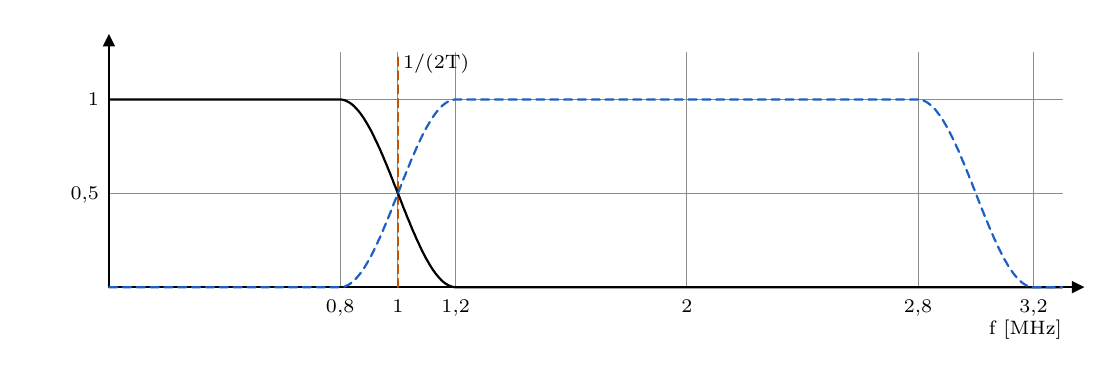
\begin{tikzpicture}[x=0.01985cm,y=-0.01985cm,line cap=round,line join=round]
\useasboundingbox (0,0) rectangle (680,200);
\path[draw=black!45,line width=0.35pt] (199.9,166) -- (199.9,16);
\path[draw=black!45,line width=0.35pt] (236.8,166) -- (236.8,16);
\path[draw=black!45,line width=0.35pt] (273.8,166) -- (273.8,16);
\path[draw=black!45,line width=0.35pt] (421.7,166) -- (421.7,16);
\path[draw=black!45,line width=0.35pt] (569.6,166) -- (569.6,16);
\path[draw=black!45,line width=0.35pt] (643.5,166) -- (643.5,16);
\path[draw=black!45,line width=0.35pt] (52,46) -- (662,46);
\path[draw=black!45,line width=0.35pt] (52,106) -- (662,106);
\path[draw=black,line width=0.7pt] (52,166) -- (670,166);
\path[fill=black,draw=none] (676,166) -- (668,162) -- (668,170) -- cycle;
\path[draw=black,line width=0.7pt] (52,166) -- (52,10);
\path[fill=black,draw=none] (52,4) -- (48,12) -- (56,12) -- cycle;
\node[anchor=base,inner sep=0pt,font=\scriptsize] at (199.9,182) {0,8};
\node[anchor=base,inner sep=0pt,font=\scriptsize] at (236.8,182) {1};
\node[anchor=base,inner sep=0pt,font=\scriptsize] at (273.8,182) {1,2};
\node[anchor=base,inner sep=0pt,font=\scriptsize] at (421.7,182) {2};
\node[anchor=base,inner sep=0pt,font=\scriptsize] at (569.6,182) {2,8};
\node[anchor=base,inner sep=0pt,font=\scriptsize] at (643.5,182) {3,2};
\node[anchor=base east,inner sep=0pt,font=\scriptsize] at (46,50) {1};
\node[anchor=base east,inner sep=0pt,font=\scriptsize] at (46,110) {0,5};
\node[anchor=base east,inner sep=0pt,font=\scriptsize] at (662,196) {f [MHz]};
\path[draw=cB,line width=0.8pt,dash pattern=on 3pt off 2pt] (236.8,166) -- (236.8,16);
\node[anchor=base west,inner sep=0pt,font=\scriptsize] at (239.8,26) {1/(2T)};
\path[draw=black,line width=0.8pt] (52,46) -- (52.8,46) -- (53.5,46) -- (54.3,46) -- (55.1,46) -- (55.8,46) -- (56.6,46) -- (57.3,46) -- (58.1,46) -- (58.9,46) -- (59.6,46) -- (60.4,46) -- (61.2,46) -- (61.9,46) -- (62.7,46) -- (63.4,46) -- (64.2,46) -- (65,46) -- (65.7,46) -- (66.5,46) -- (67.3,46) -- (68,46) -- (68.8,46) -- (69.5,46) -- (70.3,46) -- (71.1,46) -- (71.8,46) -- (72.6,46) -- (73.4,46) -- (74.1,46) -- (74.9,46) -- (75.6,46) -- (76.4,46) -- (77.2,46) -- (77.9,46) -- (78.7,46) -- (79.5,46) -- (80.2,46) -- (81,46) -- (81.7,46) -- (82.5,46) -- (83.3,46) -- (84,46) -- (84.8,46) -- (85.6,46) -- (86.3,46) -- (87.1,46) -- (87.8,46) -- (88.6,46) -- (89.4,46) -- (90.1,46) -- (90.9,46) -- (91.7,46) -- (92.4,46) -- (93.2,46) -- (93.9,46) -- (94.7,46) -- (95.5,46) -- (96.2,46) -- (97,46) -- (97.8,46) -- (98.5,46) -- (99.3,46) -- (100,46) -- (100.8,46) -- (101.6,46) -- (102.3,46) -- (103.1,46) -- (103.9,46) -- (104.6,46) -- (105.4,46) -- (106.1,46) -- (106.9,46) -- (107.7,46) -- (108.4,46) -- (109.2,46) -- (110,46) -- (110.7,46) -- (111.5,46) -- (112.2,46) -- (113,46) -- (113.8,46) -- (114.5,46) -- (115.3,46) -- (116.1,46) -- (116.8,46) -- (117.6,46) -- (118.3,46) -- (119.1,46) -- (119.9,46) -- (120.6,46) -- (121.4,46) -- (122.2,46) -- (122.9,46) -- (123.7,46) -- (124.4,46) -- (125.2,46) -- (126,46) -- (126.7,46) -- (127.5,46) -- (128.3,46) -- (129,46) -- (129.8,46) -- (130.5,46) -- (131.3,46) -- (132.1,46) -- (132.8,46) -- (133.6,46) -- (134.4,46) -- (135.1,46) -- (135.9,46) -- (136.6,46) -- (137.4,46) -- (138.2,46) -- (138.9,46) -- (139.7,46) -- (140.5,46) -- (141.2,46) -- (142,46) -- (142.7,46) -- (143.5,46) -- (144.3,46) -- (145,46) -- (145.8,46) -- (146.6,46) -- (147.3,46) -- (148.1,46) -- (148.8,46) -- (149.6,46) -- (150.4,46) -- (151.1,46) -- (151.9,46) -- (152.7,46) -- (153.4,46) -- (154.2,46) -- (154.9,46) -- (155.7,46) -- (156.5,46) -- (157.2,46) -- (158,46) -- (158.8,46) -- (159.5,46) -- (160.3,46) -- (161,46) -- (161.8,46) -- (162.6,46) -- (163.3,46) -- (164.1,46) -- (164.9,46) -- (165.6,46) -- (166.4,46) -- (167.1,46) -- (167.9,46) -- (168.7,46) -- (169.4,46) -- (170.2,46) -- (171,46) -- (171.7,46) -- (172.5,46) -- (173.2,46) -- (174,46) -- (174.8,46) -- (175.5,46) -- (176.3,46) -- (177.1,46) -- (177.8,46) -- (178.6,46) -- (179.3,46) -- (180.1,46) -- (180.9,46) -- (181.6,46) -- (182.4,46) -- (183.2,46) -- (183.9,46) -- (184.7,46) -- (185.4,46) -- (186.2,46) -- (187,46) -- (187.7,46) -- (188.5,46) -- (189.3,46) -- (190,46) -- (190.8,46) -- (191.5,46) -- (192.3,46) -- (193.1,46) -- (193.8,46) -- (194.6,46) -- (195.4,46) -- (196.1,46) -- (196.9,46) -- (197.6,46) -- (198.4,46) -- (199.2,46) -- (199.9,46) -- (200.7,46) -- (201.5,46.1) -- (202.2,46.3) -- (203,46.5) -- (203.7,46.8) -- (204.5,47.2) -- (205.3,47.6) -- (206,48) -- (206.8,48.6) -- (207.6,49.2) -- (208.3,49.8) -- (209.1,50.5) -- (209.8,51.3) -- (210.6,52.1) -- (211.4,53) -- (212.1,53.9) -- (212.9,54.9) -- (213.7,56) -- (214.4,57.1) -- (215.2,58.2) -- (215.9,59.4) -- (216.7,60.7) -- (217.5,62) -- (218.2,63.3) -- (219,64.7) -- (219.8,66.1) -- (220.5,67.6) -- (221.3,69.1) -- (222,70.7) -- (222.8,72.3) -- (223.6,73.9) -- (224.3,75.6) -- (225.1,77.2) -- (225.9,79) -- (226.6,80.7) -- (227.4,82.5) -- (228.1,84.3) -- (228.9,86.1) -- (229.7,88) -- (230.4,89.8) -- (231.2,91.7) -- (232,93.6) -- (232.7,95.5) -- (233.5,97.4) -- (234.2,99.4) -- (235,101.3) -- (235.8,103.2) -- (236.5,105.2) -- (237.3,107.1) -- (238.1,109.1) -- (238.8,111) -- (239.6,112.9) -- (240.3,114.9) -- (241.1,116.8) -- (241.9,118.7) -- (242.6,120.6) -- (243.4,122.5) -- (244.2,124.3) -- (244.9,126.2) -- (245.7,128) -- (246.4,129.8) -- (247.2,131.5) -- (248,133.3) -- (248.7,135) -- (249.5,136.7) -- (250.3,138.3) -- (251,140) -- (251.8,141.6) -- (252.5,143.1) -- (253.3,144.6) -- (254.1,146.1) -- (254.8,147.5) -- (255.6,148.9) -- (256.4,150.2) -- (257.1,151.5) -- (257.9,152.8) -- (258.6,153.9) -- (259.4,155.1) -- (260.2,156.2) -- (260.9,157.2) -- (261.7,158.2) -- (262.5,159.1) -- (263.2,160) -- (264,160.8) -- (264.7,161.6) -- (265.5,162.3) -- (266.3,162.9) -- (267,163.5) -- (267.8,164) -- (268.6,164.5) -- (269.3,164.9) -- (270.1,165.2) -- (270.8,165.5) -- (271.6,165.7) -- (272.4,165.9) -- (273.1,166) -- (273.9,166) -- (274.7,166) -- (275.4,166) -- (276.2,166) -- (276.9,166) -- (277.7,166) -- (278.5,166) -- (279.2,166) -- (280,166) -- (280.8,166) -- (281.5,166) -- (282.3,166) -- (283,166) -- (283.8,166) -- (284.6,166) -- (285.3,166) -- (286.1,166) -- (286.9,166) -- (287.6,166) -- (288.4,166) -- (289.1,166) -- (289.9,166) -- (290.7,166) -- (291.4,166) -- (292.2,166) -- (293,166) -- (293.7,166) -- (294.5,166) -- (295.2,166) -- (296,166) -- (296.8,166) -- (297.5,166) -- (298.3,166) -- (299.1,166) -- (299.8,166) -- (300.6,166) -- (301.3,166) -- (302.1,166) -- (302.9,166) -- (303.6,166) -- (304.4,166) -- (305.2,166) -- (305.9,166) -- (306.7,166) -- (307.4,166) -- (308.2,166) -- (309,166) -- (309.7,166) -- (310.5,166) -- (311.3,166) -- (312,166) -- (312.8,166) -- (313.5,166) -- (314.3,166) -- (315.1,166) -- (315.8,166) -- (316.6,166) -- (317.3,166) -- (318.1,166) -- (318.9,166) -- (319.6,166) -- (320.4,166) -- (321.2,166) -- (321.9,166) -- (322.7,166) -- (323.5,166) -- (324.2,166) -- (325,166) -- (325.7,166) -- (326.5,166) -- (327.3,166) -- (328,166) -- (328.8,166) -- (329.6,166) -- (330.3,166) -- (331.1,166) -- (331.8,166) -- (332.6,166) -- (333.4,166) -- (334.1,166) -- (334.9,166) -- (335.7,166) -- (336.4,166) -- (337.2,166) -- (337.9,166) -- (338.7,166) -- (339.5,166) -- (340.2,166) -- (341,166) -- (341.8,166) -- (342.5,166) -- (343.3,166) -- (344,166) -- (344.8,166) -- (345.6,166) -- (346.3,166) -- (347.1,166) -- (347.8,166) -- (348.6,166) -- (349.4,166) -- (350.1,166) -- (350.9,166) -- (351.7,166) -- (352.4,166) -- (353.2,166) -- (354,166) -- (354.7,166) -- (355.5,166) -- (356.2,166) -- (357,166) -- (357.8,166) -- (358.5,166) -- (359.3,166) -- (360.1,166) -- (360.8,166) -- (361.6,166) -- (362.3,166) -- (363.1,166) -- (363.9,166) -- (364.6,166) -- (365.4,166) -- (366.2,166) -- (366.9,166) -- (367.7,166) -- (368.4,166) -- (369.2,166) -- (370,166) -- (370.7,166) -- (371.5,166) -- (372.3,166) -- (373,166) -- (373.8,166) -- (374.5,166) -- (375.3,166) -- (376.1,166) -- (376.8,166) -- (377.6,166) -- (378.4,166) -- (379.1,166) -- (379.9,166) -- (380.6,166) -- (381.4,166) -- (382.2,166) -- (382.9,166) -- (383.7,166) -- (384.5,166) -- (385.2,166) -- (386,166) -- (386.7,166) -- (387.5,166) -- (388.3,166) -- (389,166) -- (389.8,166) -- (390.5,166) -- (391.3,166) -- (392.1,166) -- (392.8,166) -- (393.6,166) -- (394.4,166) -- (395.1,166) -- (395.9,166) -- (396.7,166) -- (397.4,166) -- (398.2,166) -- (398.9,166) -- (399.7,166) -- (400.5,166) -- (401.2,166) -- (402,166) -- (402.8,166) -- (403.5,166) -- (404.3,166) -- (405,166) -- (405.8,166) -- (406.6,166) -- (407.3,166) -- (408.1,166) -- (408.8,166) -- (409.6,166) -- (410.4,166) -- (411.1,166) -- (411.9,166) -- (412.7,166) -- (413.4,166) -- (414.2,166) -- (415,166) -- (415.7,166) -- (416.5,166) -- (417.2,166) -- (418,166) -- (418.8,166) -- (419.5,166) -- (420.3,166) -- (421.1,166) -- (421.8,166) -- (422.6,166) -- (423.3,166) -- (424.1,166) -- (424.9,166) -- (425.6,166) -- (426.4,166) -- (427.2,166) -- (427.9,166) -- (428.7,166) -- (429.4,166) -- (430.2,166) -- (431,166) -- (431.7,166) -- (432.5,166) -- (433.3,166) -- (434,166) -- (434.8,166) -- (435.5,166) -- (436.3,166) -- (437.1,166) -- (437.8,166) -- (438.6,166) -- (439.4,166) -- (440.1,166) -- (440.9,166) -- (441.6,166) -- (442.4,166) -- (443.2,166) -- (443.9,166) -- (444.7,166) -- (445.5,166) -- (446.2,166) -- (447,166) -- (447.7,166) -- (448.5,166) -- (449.3,166) -- (450,166) -- (450.8,166) -- (451.6,166) -- (452.3,166) -- (453.1,166) -- (453.8,166) -- (454.6,166) -- (455.4,166) -- (456.1,166) -- (456.9,166) -- (457.7,166) -- (458.4,166) -- (459.2,166) -- (459.9,166) -- (460.7,166) -- (461.5,166) -- (462.2,166) -- (463,166) -- (463.8,166) -- (464.5,166) -- (465.3,166) -- (466,166) -- (466.8,166) -- (467.6,166) -- (468.3,166) -- (469.1,166) -- (469.9,166) -- (470.6,166) -- (471.4,166) -- (472.1,166) -- (472.9,166) -- (473.7,166) -- (474.4,166) -- (475.2,166) -- (476,166) -- (476.7,166) -- (477.5,166) -- (478.2,166) -- (479,166) -- (479.8,166) -- (480.5,166) -- (481.3,166) -- (482.1,166) -- (482.8,166) -- (483.6,166) -- (484.3,166) -- (485.1,166) -- (485.9,166) -- (486.6,166) -- (487.4,166) -- (488.2,166) -- (488.9,166) -- (489.7,166) -- (490.4,166) -- (491.2,166) -- (492,166) -- (492.7,166) -- (493.5,166) -- (494.3,166) -- (495,166) -- (495.8,166) -- (496.5,166) -- (497.3,166) -- (498.1,166) -- (498.8,166) -- (499.6,166) -- (500.4,166) -- (501.1,166) -- (501.9,166) -- (502.6,166) -- (503.4,166) -- (504.2,166) -- (504.9,166) -- (505.7,166) -- (506.5,166) -- (507.2,166) -- (508,166) -- (508.7,166) -- (509.5,166) -- (510.3,166) -- (511,166) -- (511.8,166) -- (512.6,166) -- (513.3,166) -- (514.1,166) -- (514.8,166) -- (515.6,166) -- (516.4,166) -- (517.1,166) -- (517.9,166) -- (518.7,166) -- (519.4,166) -- (520.2,166) -- (520.9,166) -- (521.7,166) -- (522.5,166) -- (523.2,166) -- (524,166) -- (524.8,166) -- (525.5,166) -- (526.3,166) -- (527,166) -- (527.8,166) -- (528.6,166) -- (529.3,166) -- (530.1,166) -- (530.9,166) -- (531.6,166) -- (532.4,166) -- (533.1,166) -- (533.9,166) -- (534.7,166) -- (535.4,166) -- (536.2,166) -- (536.9,166) -- (537.7,166) -- (538.5,166) -- (539.2,166) -- (540,166) -- (540.8,166) -- (541.5,166) -- (542.3,166) -- (543.1,166) -- (543.8,166) -- (544.6,166) -- (545.3,166) -- (546.1,166) -- (546.9,166) -- (547.6,166) -- (548.4,166) -- (549.2,166) -- (549.9,166) -- (550.7,166) -- (551.4,166) -- (552.2,166) -- (553,166) -- (553.7,166) -- (554.5,166) -- (555.3,166) -- (556,166) -- (556.8,166) -- (557.5,166) -- (558.3,166) -- (559.1,166) -- (559.8,166) -- (560.6,166) -- (561.4,166) -- (562.1,166) -- (562.9,166) -- (563.6,166) -- (564.4,166) -- (565.2,166) -- (565.9,166) -- (566.7,166) -- (567.4,166) -- (568.2,166) -- (569,166) -- (569.7,166) -- (570.5,166) -- (571.3,166) -- (572,166) -- (572.8,166) -- (573.6,166) -- (574.3,166) -- (575.1,166) -- (575.8,166) -- (576.6,166) -- (577.4,166) -- (578.1,166) -- (578.9,166) -- (579.7,166) -- (580.4,166) -- (581.2,166) -- (581.9,166) -- (582.7,166) -- (583.5,166) -- (584.2,166) -- (585,166) -- (585.8,166) -- (586.5,166) -- (587.3,166) -- (588,166) -- (588.8,166) -- (589.6,166) -- (590.3,166) -- (591.1,166) -- (591.9,166) -- (592.6,166) -- (593.4,166) -- (594.1,166) -- (594.9,166) -- (595.7,166) -- (596.4,166) -- (597.2,166) -- (597.9,166) -- (598.7,166) -- (599.5,166) -- (600.2,166) -- (601,166) -- (601.8,166) -- (602.5,166) -- (603.3,166) -- (604.1,166) -- (604.8,166) -- (605.6,166) -- (606.3,166) -- (607.1,166) -- (607.9,166) -- (608.6,166) -- (609.4,166) -- (610.2,166) -- (610.9,166) -- (611.7,166) -- (612.4,166) -- (613.2,166) -- (614,166) -- (614.7,166) -- (615.5,166) -- (616.3,166) -- (617,166) -- (617.8,166) -- (618.5,166) -- (619.3,166) -- (620.1,166) -- (620.8,166) -- (621.6,166) -- (622.4,166) -- (623.1,166) -- (623.9,166) -- (624.6,166) -- (625.4,166) -- (626.2,166) -- (626.9,166) -- (627.7,166) -- (628.4,166) -- (629.2,166) -- (630,166) -- (630.7,166) -- (631.5,166) -- (632.3,166) -- (633,166) -- (633.8,166) -- (634.6,166) -- (635.3,166) -- (636.1,166) -- (636.8,166) -- (637.6,166) -- (638.4,166) -- (639.1,166) -- (639.9,166) -- (640.7,166) -- (641.4,166) -- (642.2,166) -- (642.9,166) -- (643.7,166) -- (644.5,166) -- (645.2,166) -- (646,166) -- (646.8,166) -- (647.5,166) -- (648.3,166) -- (649,166) -- (649.8,166) -- (650.6,166) -- (651.3,166) -- (652.1,166) -- (652.9,166) -- (653.6,166) -- (654.4,166) -- (655.1,166) -- (655.9,166) -- (656.7,166) -- (657.4,166) -- (658.2,166) -- (659,166) -- (659.7,166) -- (660.5,166) -- (661.2,166) -- (662,166);
\path[draw=cA,line width=0.8pt,dash pattern=on 3pt off 2pt] (52,166) -- (52.8,166) -- (53.5,166) -- (54.3,166) -- (55.1,166) -- (55.8,166) -- (56.6,166) -- (57.3,166) -- (58.1,166) -- (58.9,166) -- (59.6,166) -- (60.4,166) -- (61.2,166) -- (61.9,166) -- (62.7,166) -- (63.4,166) -- (64.2,166) -- (65,166) -- (65.7,166) -- (66.5,166) -- (67.3,166) -- (68,166) -- (68.8,166) -- (69.5,166) -- (70.3,166) -- (71.1,166) -- (71.8,166) -- (72.6,166) -- (73.4,166) -- (74.1,166) -- (74.9,166) -- (75.6,166) -- (76.4,166) -- (77.2,166) -- (77.9,166) -- (78.7,166) -- (79.5,166) -- (80.2,166) -- (81,166) -- (81.7,166) -- (82.5,166) -- (83.3,166) -- (84,166) -- (84.8,166) -- (85.6,166) -- (86.3,166) -- (87.1,166) -- (87.8,166) -- (88.6,166) -- (89.4,166) -- (90.1,166) -- (90.9,166) -- (91.7,166) -- (92.4,166) -- (93.2,166) -- (93.9,166) -- (94.7,166) -- (95.5,166) -- (96.2,166) -- (97,166) -- (97.8,166) -- (98.5,166) -- (99.3,166) -- (100,166) -- (100.8,166) -- (101.6,166) -- (102.3,166) -- (103.1,166) -- (103.9,166) -- (104.6,166) -- (105.4,166) -- (106.1,166) -- (106.9,166) -- (107.7,166) -- (108.4,166) -- (109.2,166) -- (110,166) -- (110.7,166) -- (111.5,166) -- (112.2,166) -- (113,166) -- (113.8,166) -- (114.5,166) -- (115.3,166) -- (116.1,166) -- (116.8,166) -- (117.6,166) -- (118.3,166) -- (119.1,166) -- (119.9,166) -- (120.6,166) -- (121.4,166) -- (122.2,166) -- (122.9,166) -- (123.7,166) -- (124.4,166) -- (125.2,166) -- (126,166) -- (126.7,166) -- (127.5,166) -- (128.3,166) -- (129,166) -- (129.8,166) -- (130.5,166) -- (131.3,166) -- (132.1,166) -- (132.8,166) -- (133.6,166) -- (134.4,166) -- (135.1,166) -- (135.9,166) -- (136.6,166) -- (137.4,166) -- (138.2,166) -- (138.9,166) -- (139.7,166) -- (140.5,166) -- (141.2,166) -- (142,166) -- (142.7,166) -- (143.5,166) -- (144.3,166) -- (145,166) -- (145.8,166) -- (146.6,166) -- (147.3,166) -- (148.1,166) -- (148.8,166) -- (149.6,166) -- (150.4,166) -- (151.1,166) -- (151.9,166) -- (152.7,166) -- (153.4,166) -- (154.2,166) -- (154.9,166) -- (155.7,166) -- (156.5,166) -- (157.2,166) -- (158,166) -- (158.8,166) -- (159.5,166) -- (160.3,166) -- (161,166) -- (161.8,166) -- (162.6,166) -- (163.3,166) -- (164.1,166) -- (164.9,166) -- (165.6,166) -- (166.4,166) -- (167.1,166) -- (167.9,166) -- (168.7,166) -- (169.4,166) -- (170.2,166) -- (171,166) -- (171.7,166) -- (172.5,166) -- (173.2,166) -- (174,166) -- (174.8,166) -- (175.5,166) -- (176.3,166) -- (177.1,166) -- (177.8,166) -- (178.6,166) -- (179.3,166) -- (180.1,166) -- (180.9,166) -- (181.6,166) -- (182.4,166) -- (183.2,166) -- (183.9,166) -- (184.7,166) -- (185.4,166) -- (186.2,166) -- (187,166) -- (187.7,166) -- (188.5,166) -- (189.3,166) -- (190,166) -- (190.8,166) -- (191.5,166) -- (192.3,166) -- (193.1,166) -- (193.8,166) -- (194.6,166) -- (195.4,166) -- (196.1,166) -- (196.9,166) -- (197.6,166) -- (198.4,166) -- (199.2,166) -- (199.9,166) -- (200.7,166) -- (201.5,165.9) -- (202.2,165.7) -- (203,165.5) -- (203.7,165.2) -- (204.5,164.8) -- (205.3,164.4) -- (206,164) -- (206.8,163.4) -- (207.6,162.8) -- (208.3,162.2) -- (209.1,161.5) -- (209.8,160.7) -- (210.6,159.9) -- (211.4,159) -- (212.1,158.1) -- (212.9,157.1) -- (213.7,156) -- (214.4,154.9) -- (215.2,153.8) -- (215.9,152.6) -- (216.7,151.3) -- (217.5,150) -- (218.2,148.7) -- (219,147.3) -- (219.8,145.9) -- (220.5,144.4) -- (221.3,142.9) -- (222,141.3) -- (222.8,139.7) -- (223.6,138.1) -- (224.3,136.4) -- (225.1,134.8) -- (225.9,133) -- (226.6,131.3) -- (227.4,129.5) -- (228.1,127.7) -- (228.9,125.9) -- (229.7,124) -- (230.4,122.2) -- (231.2,120.3) -- (232,118.4) -- (232.7,116.5) -- (233.5,114.6) -- (234.2,112.6) -- (235,110.7) -- (235.8,108.8) -- (236.5,106.8) -- (237.3,104.9) -- (238.1,102.9) -- (238.8,101) -- (239.6,99.1) -- (240.3,97.1) -- (241.1,95.2) -- (241.9,93.3) -- (242.6,91.4) -- (243.4,89.5) -- (244.2,87.7) -- (244.9,85.8) -- (245.7,84) -- (246.4,82.2) -- (247.2,80.5) -- (248,78.7) -- (248.7,77) -- (249.5,75.3) -- (250.3,73.7) -- (251,72) -- (251.8,70.4) -- (252.5,68.9) -- (253.3,67.4) -- (254.1,65.9) -- (254.8,64.5) -- (255.6,63.1) -- (256.4,61.8) -- (257.1,60.5) -- (257.9,59.2) -- (258.6,58.1) -- (259.4,56.9) -- (260.2,55.8) -- (260.9,54.8) -- (261.7,53.8) -- (262.5,52.9) -- (263.2,52) -- (264,51.2) -- (264.7,50.4) -- (265.5,49.7) -- (266.3,49.1) -- (267,48.5) -- (267.8,48) -- (268.6,47.5) -- (269.3,47.1) -- (270.1,46.8) -- (270.8,46.5) -- (271.6,46.3) -- (272.4,46.1) -- (273.1,46) -- (273.9,46) -- (274.7,46) -- (275.4,46) -- (276.2,46) -- (276.9,46) -- (277.7,46) -- (278.5,46) -- (279.2,46) -- (280,46) -- (280.8,46) -- (281.5,46) -- (282.3,46) -- (283,46) -- (283.8,46) -- (284.6,46) -- (285.3,46) -- (286.1,46) -- (286.9,46) -- (287.6,46) -- (288.4,46) -- (289.1,46) -- (289.9,46) -- (290.7,46) -- (291.4,46) -- (292.2,46) -- (293,46) -- (293.7,46) -- (294.5,46) -- (295.2,46) -- (296,46) -- (296.8,46) -- (297.5,46) -- (298.3,46) -- (299.1,46) -- (299.8,46) -- (300.6,46) -- (301.3,46) -- (302.1,46) -- (302.9,46) -- (303.6,46) -- (304.4,46) -- (305.2,46) -- (305.9,46) -- (306.7,46) -- (307.4,46) -- (308.2,46) -- (309,46) -- (309.7,46) -- (310.5,46) -- (311.3,46) -- (312,46) -- (312.8,46) -- (313.5,46) -- (314.3,46) -- (315.1,46) -- (315.8,46) -- (316.6,46) -- (317.3,46) -- (318.1,46) -- (318.9,46) -- (319.6,46) -- (320.4,46) -- (321.2,46) -- (321.9,46) -- (322.7,46) -- (323.5,46) -- (324.2,46) -- (325,46) -- (325.7,46) -- (326.5,46) -- (327.3,46) -- (328,46) -- (328.8,46) -- (329.6,46) -- (330.3,46) -- (331.1,46) -- (331.8,46) -- (332.6,46) -- (333.4,46) -- (334.1,46) -- (334.9,46) -- (335.7,46) -- (336.4,46) -- (337.2,46) -- (337.9,46) -- (338.7,46) -- (339.5,46) -- (340.2,46) -- (341,46) -- (341.8,46) -- (342.5,46) -- (343.3,46) -- (344,46) -- (344.8,46) -- (345.6,46) -- (346.3,46) -- (347.1,46) -- (347.8,46) -- (348.6,46) -- (349.4,46) -- (350.1,46) -- (350.9,46) -- (351.7,46) -- (352.4,46) -- (353.2,46) -- (354,46) -- (354.7,46) -- (355.5,46) -- (356.2,46) -- (357,46) -- (357.8,46) -- (358.5,46) -- (359.3,46) -- (360.1,46) -- (360.8,46) -- (361.6,46) -- (362.3,46) -- (363.1,46) -- (363.9,46) -- (364.6,46) -- (365.4,46) -- (366.2,46) -- (366.9,46) -- (367.7,46) -- (368.4,46) -- (369.2,46) -- (370,46) -- (370.7,46) -- (371.5,46) -- (372.3,46) -- (373,46) -- (373.8,46) -- (374.5,46) -- (375.3,46) -- (376.1,46) -- (376.8,46) -- (377.6,46) -- (378.4,46) -- (379.1,46) -- (379.9,46) -- (380.6,46) -- (381.4,46) -- (382.2,46) -- (382.9,46) -- (383.7,46) -- (384.5,46) -- (385.2,46) -- (386,46) -- (386.7,46) -- (387.5,46) -- (388.3,46) -- (389,46) -- (389.8,46) -- (390.5,46) -- (391.3,46) -- (392.1,46) -- (392.8,46) -- (393.6,46) -- (394.4,46) -- (395.1,46) -- (395.9,46) -- (396.7,46) -- (397.4,46) -- (398.2,46) -- (398.9,46) -- (399.7,46) -- (400.5,46) -- (401.2,46) -- (402,46) -- (402.8,46) -- (403.5,46) -- (404.3,46) -- (405,46) -- (405.8,46) -- (406.6,46) -- (407.3,46) -- (408.1,46) -- (408.8,46) -- (409.6,46) -- (410.4,46) -- (411.1,46) -- (411.9,46) -- (412.7,46) -- (413.4,46) -- (414.2,46) -- (415,46) -- (415.7,46) -- (416.5,46) -- (417.2,46) -- (418,46) -- (418.8,46) -- (419.5,46) -- (420.3,46) -- (421.1,46) -- (421.8,46) -- (422.6,46) -- (423.3,46) -- (424.1,46) -- (424.9,46) -- (425.6,46) -- (426.4,46) -- (427.2,46) -- (427.9,46) -- (428.7,46) -- (429.4,46) -- (430.2,46) -- (431,46) -- (431.7,46) -- (432.5,46) -- (433.3,46) -- (434,46) -- (434.8,46) -- (435.5,46) -- (436.3,46) -- (437.1,46) -- (437.8,46) -- (438.6,46) -- (439.4,46) -- (440.1,46) -- (440.9,46) -- (441.6,46) -- (442.4,46) -- (443.2,46) -- (443.9,46) -- (444.7,46) -- (445.5,46) -- (446.2,46) -- (447,46) -- (447.7,46) -- (448.5,46) -- (449.3,46) -- (450,46) -- (450.8,46) -- (451.6,46) -- (452.3,46) -- (453.1,46) -- (453.8,46) -- (454.6,46) -- (455.4,46) -- (456.1,46) -- (456.9,46) -- (457.7,46) -- (458.4,46) -- (459.2,46) -- (459.9,46) -- (460.7,46) -- (461.5,46) -- (462.2,46) -- (463,46) -- (463.8,46) -- (464.5,46) -- (465.3,46) -- (466,46) -- (466.8,46) -- (467.6,46) -- (468.3,46) -- (469.1,46) -- (469.9,46) -- (470.6,46) -- (471.4,46) -- (472.1,46) -- (472.9,46) -- (473.7,46) -- (474.4,46) -- (475.2,46) -- (476,46) -- (476.7,46) -- (477.5,46) -- (478.2,46) -- (479,46) -- (479.8,46) -- (480.5,46) -- (481.3,46) -- (482.1,46) -- (482.8,46) -- (483.6,46) -- (484.3,46) -- (485.1,46) -- (485.9,46) -- (486.6,46) -- (487.4,46) -- (488.2,46) -- (488.9,46) -- (489.7,46) -- (490.4,46) -- (491.2,46) -- (492,46) -- (492.7,46) -- (493.5,46) -- (494.3,46) -- (495,46) -- (495.8,46) -- (496.5,46) -- (497.3,46) -- (498.1,46) -- (498.8,46) -- (499.6,46) -- (500.4,46) -- (501.1,46) -- (501.9,46) -- (502.6,46) -- (503.4,46) -- (504.2,46) -- (504.9,46) -- (505.7,46) -- (506.5,46) -- (507.2,46) -- (508,46) -- (508.7,46) -- (509.5,46) -- (510.3,46) -- (511,46) -- (511.8,46) -- (512.6,46) -- (513.3,46) -- (514.1,46) -- (514.8,46) -- (515.6,46) -- (516.4,46) -- (517.1,46) -- (517.9,46) -- (518.7,46) -- (519.4,46) -- (520.2,46) -- (520.9,46) -- (521.7,46) -- (522.5,46) -- (523.2,46) -- (524,46) -- (524.8,46) -- (525.5,46) -- (526.3,46) -- (527,46) -- (527.8,46) -- (528.6,46) -- (529.3,46) -- (530.1,46) -- (530.9,46) -- (531.6,46) -- (532.4,46) -- (533.1,46) -- (533.9,46) -- (534.7,46) -- (535.4,46) -- (536.2,46) -- (536.9,46) -- (537.7,46) -- (538.5,46) -- (539.2,46) -- (540,46) -- (540.8,46) -- (541.5,46) -- (542.3,46) -- (543.1,46) -- (543.8,46) -- (544.6,46) -- (545.3,46) -- (546.1,46) -- (546.9,46) -- (547.6,46) -- (548.4,46) -- (549.2,46) -- (549.9,46) -- (550.7,46) -- (551.4,46) -- (552.2,46) -- (553,46) -- (553.7,46) -- (554.5,46) -- (555.3,46) -- (556,46) -- (556.8,46) -- (557.5,46) -- (558.3,46) -- (559.1,46) -- (559.8,46) -- (560.6,46) -- (561.4,46) -- (562.1,46) -- (562.9,46) -- (563.6,46) -- (564.4,46) -- (565.2,46) -- (565.9,46) -- (566.7,46) -- (567.4,46) -- (568.2,46) -- (569,46) -- (569.7,46) -- (570.5,46) -- (571.3,46.2) -- (572,46.3) -- (572.8,46.6) -- (573.6,46.9) -- (574.3,47.2) -- (575.1,47.6) -- (575.8,48.1) -- (576.6,48.7) -- (577.4,49.3) -- (578.1,49.9) -- (578.9,50.6) -- (579.7,51.4) -- (580.4,52.2) -- (581.2,53.1) -- (581.9,54.1) -- (582.7,55.1) -- (583.5,56.1) -- (584.2,57.3) -- (585,58.4) -- (585.8,59.6) -- (586.5,60.9) -- (587.3,62.2) -- (588,63.5) -- (588.8,64.9) -- (589.6,66.4) -- (590.3,67.8) -- (591.1,69.4) -- (591.9,70.9) -- (592.6,72.5) -- (593.4,74.1) -- (594.1,75.8) -- (594.9,77.5) -- (595.7,79.2) -- (596.4,81) -- (597.2,82.8) -- (597.9,84.6) -- (598.7,86.4) -- (599.5,88.2) -- (600.2,90.1) -- (601,92) -- (601.8,93.9) -- (602.5,95.8) -- (603.3,97.7) -- (604.1,99.7) -- (604.8,101.6) -- (605.6,103.5) -- (606.3,105.5) -- (607.1,107.4) -- (607.9,109.4) -- (608.6,111.3) -- (609.4,113.2) -- (610.2,115.2) -- (610.9,117.1) -- (611.7,119) -- (612.4,120.9) -- (613.2,122.7) -- (614,124.6) -- (614.7,126.4) -- (615.5,128.3) -- (616.3,130) -- (617,131.8) -- (617.8,133.6) -- (618.5,135.3) -- (619.3,136.9) -- (620.1,138.6) -- (620.8,140.2) -- (621.6,141.8) -- (622.4,143.3) -- (623.1,144.8) -- (623.9,146.3) -- (624.6,147.7) -- (625.4,149.1) -- (626.2,150.4) -- (626.9,151.7) -- (627.7,152.9) -- (628.4,154.1) -- (629.2,155.3) -- (630,156.3) -- (630.7,157.4) -- (631.5,158.3) -- (632.3,159.3) -- (633,160.1) -- (633.8,160.9) -- (634.6,161.7) -- (635.3,162.4) -- (636.1,163) -- (636.8,163.6) -- (637.6,164.1) -- (638.4,164.6) -- (639.1,165) -- (639.9,165.3) -- (640.7,165.6) -- (641.4,165.8) -- (642.2,165.9) -- (642.9,166) -- (643.7,166) -- (644.5,166) -- (645.2,166) -- (646,166) -- (646.8,166) -- (647.5,166) -- (648.3,166) -- (649,166) -- (649.8,166) -- (650.6,166) -- (651.3,166) -- (652.1,166) -- (652.9,166) -- (653.6,166) -- (654.4,166) -- (655.1,166) -- (655.9,166) -- (656.7,166) -- (657.4,166) -- (658.2,166) -- (659,166) -- (659.7,166) -- (660.5,166) -- (661.2,166) -- (662,166);
\end{tikzpicture}\end{center}
\begin{itemize}
\item 0,8 MHz-ig 1, onnan koszinuszosan 0-ra 1,2 MHz-ig, 1 MHz-en 0,5. A lecsengés az 1 MHz-es pontra szimmetrikus.
\item A $1/T=2$ MHz-cel eltolt másolat lecsengése a 0,8 és 1,2 MHz közötti részt pontosan kiegészíti.
\end{itemize}
\end{rajz}
\begin{eredmeny}

\begin{center}\adjustbox{max width=\linewidth}{$\displaystyle \text{a) }T=0{,}5\ \mu\text{s}\qquad\text{b) emelt koszinusz}\qquad\text{c) }4\ \text{Mbit/s}\qquad\text{d) }\alpha=20\%$}\end{center}
\end{eredmeny}

% Generálva: html/build_tex.js (o04.js). Kézzel ne szerkeszd, a forrás a html/data mappa.
\setcounter{chapter}{3}
\chapter{\texorpdfstring{Mintavételezés és kvantálás}{Mintavételezés és kvantálás}}\label{f4}
Mi jelenik meg a kimeneten, és milyen mintavételi frekvenciák választhatók. Négyszögjelnél a páratlan felharmonikusok mind „képeket” adnak.

\section{Alapok, egyszerűen}
\subsection{\texorpdfstring{A1. Jelölések és a lánc}{A1. Jelölések és a lánc}}\label{b4-jel}
\par\noindent{\small\renewcommand{\arraystretch}{1.25}\begin{tabularx}{\linewidth}{@{}>{\raggedright\arraybackslash}X>{\raggedright\arraybackslash}X@{}}\toprule
\textbf{Jel} & \textbf{Jelentés}\\\midrule
undefined & mintavételi frekvencia\\
undefined & a jel legkisebb és legnagyobb frekvenciája\\
undefined & a jel sávszélessége, undefined\\
undefined & a kvantáló bitszáma\\
undefined & a jel csúcstényezője (szinusznál undefined)\\
\bottomrule\end{tabularx}}\par

A lánc: \textbf{előszűrő $\to$ mintavevő $\to$ \ldots{} $\to$ visszaállító (utó)szűrő}. Egy $f$ frekvenciájú bemenet a mintavétel után az $nf_s\pm f$ frekvenciákon is megjelenik (álképek). Egy kimenő összetevő amplitúdója: bemenő amplitúdó $\times$ az előszűrő átvitele az eredeti frekvencián $\times$ az utószűrő átvitele a kimenő frekvencián. A 40 dB-es csillapítás 0,01-es szorzó, mert $20\lg0{,}01=-40$.

\subsection{\texorpdfstring{A2. Sáváteresztő mintavétel és kvantálási zaj}{A2. Sáváteresztő mintavétel és kvantálási zaj}}\label{b4-kepl}
Sáváteresztő jelnél a megengedett tartományok egész $k$-ra:

\begin{center}\adjustbox{max width=\linewidth}{$\displaystyle \frac{2f_H}{k}\le f_s\le\frac{2f_L}{k-1}\qquad1\le k\le\left\lfloor\frac{f_H}{B}\right\rfloor$}\end{center}

Egyenletes kvantálásnál a jel-zaj viszony dB-ben:

\begin{center}\adjustbox{max width=\linewidth}{$\displaystyle \text{SNR}=10\lg\frac{3}{C^2}+10\lg\frac{f_s}{2B_z}+6{,}02\,n$}\end{center}

Az első tag a jel alakja (szinusznál $10\lg1{,}5=1{,}76$ dB), a második a túlmintavételezés nyeresége ($B_z$ a visszaállító szűrő sávja, ennyi zaj marad meg a $f_s/2$ szélességben szétterülő zajból), a harmadik a bitszám.

% ------------------------------------------------------------------
\section{\texorpdfstring{4.1. feladat: Négyszögjelből csak 1, 3, 7, 9 kHz}{4.1. feladat: Négyszögjelből csak 1, 3, 7, 9 kHz}}\label{o4_01}
\setcounter{lepes}{0}
\begin{feladat}{4.1. feladat}
A be- és kimenő szűrő ideális aluláteresztő, de más a sávjuk. A bemenet 1 kHz-es négyszögjel (páratlan felharmonikusok), a kimeneten csak 1, 3, 7, 9 kHz jelenik meg. a) A szűrők sávja? b) A mintavételi frekvencia?

{\footnotesize\sffamily Forrás: 5-ösöm 12. oldal $\cdot$ 5o\_12\_1. Címkék: vizsga}
\end{feladat}
\begin{keresunk}
\begin{itemize}
\item a) $B_\text{be}$ (a bemenő szűrő sávja), $B_\text{ki}$: a két szűrő határfrekvenciája
\item b) $f_s$ (mintavételi frekvencia)
\end{itemize}
\end{keresunk}
\begin{jeloles}
\begin{jeltabla}
$B_\text{be}$ & a bemenő szűrő sávja & \emph{keresett}\\
$B_\text{ki}$ & a kimenő szűrő sávja & \emph{keresett}\\
$f_s$ & mintavételi frekvencia & \emph{keresett}\\
\end{jeltabla}
\par\smallskip\textbf{Adott még:}
\begin{itemize}
\item a bemenet összetevői: $1,\ 3,\ 5,\ 7,\ 9,\ \ldots$ kHz (az 1 kHz-es négyszögjel páratlan felharmonikusai)
\item a kimenet: csak $1,\ 3,\ 7,\ 9$ kHz
\end{itemize}
\end{jeloles}

\lepes{a) Az előszűrő}
A 3 kHz megjelenik, tehát átjutott. Ha az 5 kHz átjutna, a kimeneten is ott lenne (a kimenő szűrő a 9 kHz-et is átengedi). Tehát az előszűrő a 3-at átengedi, az 5-öt nem.

\begin{center}\adjustbox{max width=\linewidth}{$\displaystyle 3\ \text{kHz}<B_\text{be}<5\ \text{kHz}$}\end{center}
\jegyzet{ellenőrzés}{}

\lepes{b) A mintavételi frekvencia}
A mintavevőhöz csak az 1 és a 3 kHz jut el, ezek álképei $f_s\pm1$ és $f_s\pm3$. A 7 és a 9 kHz nem lehet eredeti összetevő (az előszűrő levágta), tehát álkép.

\begin{center}\adjustbox{max width=\linewidth}{$\displaystyle f_s-3=7\quad\text{és}\quad f_s-1=9\ \Rightarrow\ f_s=10\ \text{kHz}$}\end{center}
\jegyzet{behelyettesítés}{}

\begin{center}\adjustbox{max width=\linewidth}{$\displaystyle f_s=8:\ 8-3=5\ \text{kHz is lenne}\qquad f_s=12:\ 12-3=9,\ 12-1=11,\ \text{a 7 hiányozna}$}\end{center}
\jegyzet{ellenőrzés}{más érték nem jó}

\lepes{a) A kimenő szűrő}
$f_s=10$ kHz-nél a következő álképek $10+1=11$ és $10+3=13$ kHz. A 9 kHz átjut, a 11 nem.

\begin{center}\adjustbox{max width=\linewidth}{$\displaystyle 9\ \text{kHz}<B_\text{ki}<11\ \text{kHz}$}\end{center}
\jegyzet{ellenőrzés}{}

\begin{rajz}
\textbf{A kimenet összetevői, f\_s = 10 kHz}\par
\begin{center}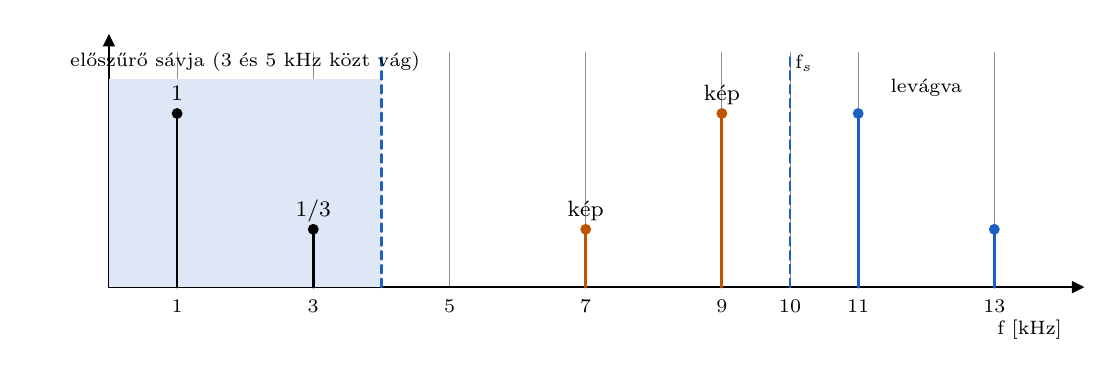
\begin{tikzpicture}[x=0.01985cm,y=-0.01985cm,line cap=round,line join=round]
\useasboundingbox (0,0) rectangle (680,200);
\path[draw=black!45,line width=0.35pt] (95.6,166) -- (95.6,16);
\path[draw=black!45,line width=0.35pt] (182.7,166) -- (182.7,16);
\path[draw=black!45,line width=0.35pt] (269.9,166) -- (269.9,16);
\path[draw=black!45,line width=0.35pt] (357,166) -- (357,16);
\path[draw=black!45,line width=0.35pt] (444.1,166) -- (444.1,16);
\path[draw=black!45,line width=0.35pt] (487.7,166) -- (487.7,16);
\path[draw=black!45,line width=0.35pt] (531.3,166) -- (531.3,16);
\path[draw=black!45,line width=0.35pt] (618.4,166) -- (618.4,16);
\path[draw=black,line width=0.7pt] (52,166) -- (670,166);
\path[fill=black,draw=none] (676,166) -- (668,162) -- (668,170) -- cycle;
\path[draw=black,line width=0.7pt] (52,166) -- (52,10);
\path[fill=black,draw=none] (52,4) -- (48,12) -- (56,12) -- cycle;
\node[anchor=base,inner sep=0pt,font=\scriptsize] at (95.6,182) {1};
\node[anchor=base,inner sep=0pt,font=\scriptsize] at (182.7,182) {3};
\node[anchor=base,inner sep=0pt,font=\scriptsize] at (269.9,182) {5};
\node[anchor=base,inner sep=0pt,font=\scriptsize] at (357,182) {7};
\node[anchor=base,inner sep=0pt,font=\scriptsize] at (444.1,182) {9};
\node[anchor=base,inner sep=0pt,font=\scriptsize] at (487.7,182) {10};
\node[anchor=base,inner sep=0pt,font=\scriptsize] at (531.3,182) {11};
\node[anchor=base,inner sep=0pt,font=\scriptsize] at (618.4,182) {13};
\node[anchor=base east,inner sep=0pt,font=\scriptsize] at (662,196) {f [kHz]};
\path[fill=cA!15,draw=none] (52,166) -- (52,32.7) -- (226.3,32.7) -- (226.3,166) -- cycle;
\path[draw=cB,line width=0.8pt,dash pattern=on 3pt off 2pt] (487.7,166) -- (487.7,16);
\node[anchor=base west,inner sep=0pt,font=\scriptsize] at (490.7,26) {f$_s$};
\path[draw=cA,line width=0.8pt,dash pattern=on 3pt off 2pt] (226.3,166) -- (226.3,16);
\path[draw=cA,line width=0.8pt,dash pattern=on 3pt off 2pt] (487.7,166) -- (487.7,16);
\path[draw=black,line width=0.8pt,line width=0.99pt] (95.6,166) -- (95.6,54.9);
\path[fill=black,draw=none] (95.6,54.9) circle[radius=0.069cm];
\node[anchor=base,inner sep=0pt,font=\footnotesize] at (95.6,46.9) {1};
\path[draw=black,line width=0.8pt,line width=0.99pt] (182.7,166) -- (182.7,129);
\path[fill=black,draw=none] (182.7,129) circle[radius=0.069cm];
\node[anchor=base,inner sep=0pt,font=\footnotesize] at (182.7,121) {1/3};
\path[draw=cB,line width=0.8pt,line width=0.99pt] (357,166) -- (357,129);
\path[fill=cB,draw=none] (357,129) circle[radius=0.069cm];
\node[anchor=base,inner sep=0pt,font=\footnotesize] at (357,121) {kép};
\path[draw=cB,line width=0.8pt,line width=0.99pt] (444.1,166) -- (444.1,54.9);
\path[fill=cB,draw=none] (444.1,54.9) circle[radius=0.069cm];
\node[anchor=base,inner sep=0pt,font=\footnotesize] at (444.1,46.9) {kép};
\path[draw=cA,line width=0.8pt,line width=0.99pt] (531.3,166) -- (531.3,54.9);
\path[fill=cA,draw=none] (531.3,54.9) circle[radius=0.069cm];
\path[draw=cA,line width=0.8pt,line width=0.99pt] (618.4,166) -- (618.4,129);
\path[fill=cA,draw=none] (618.4,129) circle[radius=0.069cm];
\node[anchor=base,inner sep=0pt,font=\scriptsize] at (139.1,24.9) {előszűrő sávja (3 és 5 kHz közt vág)};
\node[anchor=base,inner sep=0pt,font=\scriptsize] at (574.9,41.6) {levágva};
\end{tikzpicture}\end{center}
\begin{itemize}
\item A négyszögjel összetevői 1, 3, 5, \ldots{} kHz-en, amplitúdójuk $1/k$ arányú. Az előszűrő csak az 1 és a 3 kHz-et engedi át.
\item $f_s=10$ kHz körül tükröződnek: $10-3=7$ és $10-1=9$ kHz (kép), a $10+1=11$ és $10+3=13$ kHz-et a kimenő szűrő levágja.
\end{itemize}
\end{rajz}
\begin{eredmeny}

\begin{center}\adjustbox{max width=\linewidth}{$\displaystyle \text{a) }3<B_\text{be}<5\ \text{kHz},\ 9<B_\text{ki}<11\ \text{kHz}\qquad\text{b) }f_s=10\ \text{kHz}$}\end{center}
\end{eredmeny}


% ------------------------------------------------------------------
\section{\texorpdfstring{4.2. feladat: 8 kHz, 40 dB-es szűrők, négyszögjel a bemeneten}{4.2. feladat: 8 kHz, 40 dB-es szűrők, négyszögjel a bemeneten}}\label{o4_02}
\setcounter{lepes}{0}
\begin{feladat}{4.2. feladat}
8 kHz-es rendszer, 4 kHz-es aluláteresztő elő- és utószűrő 40 dB-es zárócsillapítással, a 2 V-os 1,5 kHz-es jelet amplitúdóhelyesen viszi át. a) Mi jelenik meg 3,5 kHz-es szinuszra? b) Milyen 2 mV-nál nagyobb komponensek jönnek 1,5 kHz-es (2 V-os) négyszögjelre? c) És előszűrő nélkül?

{\footnotesize\sffamily Forrás: 5-ösöm 12. oldal $\cdot$ 5o\_12\_2. Címkék: vizsga, nehezebb, javítás}
\end{feladat}
\begin{keresunk}
\begin{itemize}
\item a), b), c) a kimenet összetevői és amplitúdóik
\end{itemize}
\end{keresunk}
\begin{jeloles}
\begin{jeltabla}
$\ca{f_s}$ & mintavételi frekvencia & $8$\,kHz\\
$n$ & tetszőleges egész szám (hányadik mintavételi többszörös) & \\
$\hat U$ & a négyszögjel amplitúdója & \\
$k$ & a felharmonikus (páratlan) sorszáma & \\
\end{jeltabla}
\par\smallskip\textbf{Adott még:}
\begin{itemize}
\item mindkét szűrő 4 kHz alatt 1-szeres, felette 0,01-szeres (40 dB)
\item a) 2 V-os, 3,5 kHz-es szinusz
\item b) 2 V-os, 1,5 kHz-es négyszögjel
\end{itemize}
\end{jeloles}

\lepes{a) Szinusz 3,5 kHz-en}
A 3,5 kHz a sávban van, az előszűrő 2 V-tal átengedi. A mintavétel után a $n\cdot8\pm3{,}5$ kHz-es álképek is megjelennek, ugyancsak 2 V-tal. Az utószűrő a sávon kívülieket 0,01-szeresre csillapítja.

\begin{center}\adjustbox{max width=\linewidth}{$\displaystyle 3{,}5\ \text{kHz: }2\ \text{V}$}\end{center}
\jegyzet{számérték}{a sávban}

\begin{center}\adjustbox{max width=\linewidth}{$\displaystyle 4{,}5,\ 11{,}5,\ 12{,}5,\ 19{,}5,\ \ldots\ \text{kHz: }2\cdot0{,}01=20\ \text{mV}$}\end{center}
\jegyzet{számérték}{$8\pm3{,}5$, $16\pm3{,}5$, \ldots{}}

\lepes{b) A négyszögjel összetevői}
A $\hat U$ amplitúdójú négyszögjel $k$-adik (páratlan) felharmonikusa $4\hat U/(\pi k)$. A 4 kHz felettieket az előszűrő 0,01-szeresre csökkenti.

\begin{center}\adjustbox{max width=\linewidth}{$\displaystyle 1{,}5\ \text{kHz: }\frac{4\cdot2}{\pi}=2{,}55\ \text{V}$}\end{center}
\jegyzet{számérték}{$k=1$, átjut}

\begin{center}\adjustbox{max width=\linewidth}{$\displaystyle 4{,}5\ \text{kHz: }0{,}85\cdot0{,}01=8{,}5\ \text{mV}\qquad7{,}5:\ 5{,}1\ \text{mV}\qquad10{,}5:\ 3{,}6\ \text{mV}\qquad13{,}5:\ 2{,}8\ \text{mV}$}\end{center}
\jegyzet{számérték}{$k=3,5,7,9$, az előszűrő után}

\lepes{b) Hová lapolódnak?}
Mindegyik a $8$ kHz többszöröseitől mért távolságára, a sávba is. Az utószűrő a sávbelieket átengedi, a sávon kívülieket még egyszer 0,01-gyel szorozza.

\begin{center}\adjustbox{max width=\linewidth}{$\displaystyle 8-4{,}5=3{,}5\qquad8-7{,}5=0{,}5\qquad10{,}5-8=2{,}5\qquad16-13{,}5=2{,}5\ \text{kHz}$}\end{center}
\jegyzet{számérték}{a sávba esnek}

\begin{center}\adjustbox{max width=\linewidth}{$\displaystyle n\cdot8\pm1{,}5\ \text{kHz (6,5, 9,5, 14,5, \ldots{}): }2{,}55\cdot0{,}01=25\ \text{mV}$}\end{center}
\jegyzet{számérték}{az alapharmonikus álképei}

\begin{center}\adjustbox{max width=\linewidth}{$\displaystyle 4{,}5\ \text{kHz eredetiben: }8{,}5\ \text{mV}\cdot0{,}01\approx0{,}1\ \text{mV}<2\ \text{mV}$}\end{center}
\jegyzet{ellenőrzés}{kétszer csillapítva elhanyagolható}

\lepes{c) Előszűrő nélkül}
Ugyanazok a frekvenciák jelennek meg, de a felharmonikusok csillapítatlanul lapolódnak a sávba.

\begin{center}\adjustbox{max width=\linewidth}{$\displaystyle 3{,}5\ \text{kHz: }0{,}85\ \text{V}\qquad0{,}5\ \text{kHz: }0{,}51\ \text{V}\qquad2{,}5\ \text{kHz: }0{,}36\ \text{és }0{,}28\ \text{V}$}\end{center}
\jegyzet{számérték}{a 4,5, 7,5, 10,5 és 13,5 kHz-es felharmonikusból}
\begin{tipp}[A gyűjtemény megoldása]
A gyűjtemény b)-re csak „$\pm(1{,}5+kf_0)$, $k$ páratlan” vázlatot ad, c)-re szerinte „szűrő nélkül is megkapjuk az összes jelet”.
\end{tipp}
\begin{figyelem}[Javítás]
A frekvenciák halmaza előszűrő nélkül valóban nem változik, de a sávba lapolódó összetevők a néhány mV helyett több száz mV-osak: ez erős, hallható torzítás.
\end{figyelem}
\begin{eredmeny}

\begin{center}\adjustbox{max width=\linewidth}{$\displaystyle \text{a) }3{,}5\ \text{kHz }2\ \text{V},\ n\cdot8\pm3{,}5\ \text{kHz }20\ \text{mV}$}\end{center}

\begin{center}\adjustbox{max width=\linewidth}{$\displaystyle \text{b) }1{,}5\ \text{kHz }2{,}55\ \text{V},\ 0{,}5,\ 2{,}5,\ 3{,}5\ \text{kHz néhány mV},\ n\cdot8\pm1{,}5\ \text{kHz }25\ \text{mV}\qquad\text{c) ugyanezek a frekvenciák, a sávban tized voltos nagyságban}$}\end{center}
\end{eredmeny}


% ------------------------------------------------------------------
\section{\texorpdfstring{4.3. feladat: 1,45 kHz előszűrő nélkül (hivatalos válaszok)}{4.3. feladat: 1,45 kHz előszűrő nélkül (hivatalos válaszok)}}\label{o4_03}
\setcounter{lepes}{0}
\begin{feladat}{4.3. feladat}
8 kHz-es rendszer, jó 4 kHz-es visszaállító szűrő, de nincs előszűrő. a) Kimenet 2 V-os 1,45 kHz-re? b) Lesz-e 9,45 kHz-es összetevő? c) Mi jelenik meg 4,45 kHz-es bemenetre? d) És 1,45 kHz-es négyszögjelre?

{\footnotesize\sffamily Forrás: 5-ösöm 13. oldal $\cdot$ 5o\_13\_1. Címkék: vizsga}
\end{feladat}
\begin{keresunk}
\begin{itemize}
\item a), b), c), d) a kimenet összetevői
\end{itemize}
\end{keresunk}
\begin{jeloles}
\begin{jeltabla}
$\ca{f_s}$ & mintavételi frekvencia & $8$\,kHz\\
$k$ & a felharmonikus (páratlan) sorszáma & \\
$n$ & tetszőleges egész szám (hányadik mintavételi többszörös) & \\
\end{jeltabla}
\par\smallskip\textbf{Adott még:}
\begin{itemize}
\item a visszaállító szűrő jó (ideálisnak vehető), 4 kHz-ig enged át
\end{itemize}
\end{jeloles}

\lepes{a) 1,45 kHz}
A sávban van, a szűrő átengedi. Az álképei ($8\pm1{,}45$, \ldots{}) mind 4 kHz felett vannak, a jó szűrő levágja őket.

\begin{center}\adjustbox{max width=\linewidth}{$\displaystyle 1{,}45\ \text{kHz},\ 2\ \text{V}$}\end{center}
\jegyzet{számérték}{}

\lepes{b) 9,45 kHz}
A mintavétel után van ilyen összetevő, mert $8+1{,}45=9{,}45$. A kimeneten nincs, mert a visszaállító szűrő eltávolítja.

\begin{center}\adjustbox{max width=\linewidth}{$\displaystyle 8+1{,}45=9{,}45\ \text{kHz}>4\ \text{kHz}$}\end{center}
\jegyzet{számérték}{levágva}

\lepes{c) 4,45 kHz}
Előszűrő nincs, a 4,45 kHz bejut. Az álképe a sávba esik, és a kimenő szűrő ezt nem tudja megkülönböztetni egy valódi 3,55 kHz-es jeltől.

\begin{center}\adjustbox{max width=\linewidth}{$\displaystyle 8-4{,}45=3{,}55\ \text{kHz},\ 2\ \text{V}$}\end{center}
\jegyzet{számérték}{hamis összetevő, a jó szűrő sem távolítja el}

\lepes{d) Négyszögjel 1,45 kHz-en}
A felharmonikusok ($k\cdot1{,}45$ kHz, $k$ páratlan) mind bejutnak, és a sávba lapolódnak. A $k$-adik amplitúdója a négyszögjel amplitúdójának $4/(\pi k)$-szorosa.

\begin{center}\adjustbox{max width=\linewidth}{$\displaystyle 4{,}35\to3{,}65\qquad7{,}25\to0{,}75\qquad10{,}15\to2{,}15\qquad13{,}05\to2{,}95\qquad15{,}95\to0{,}05\ \text{kHz}$}\end{center}
\jegyzet{számérték}{$|n\cdot8-k\cdot1{,}45|$}
\begin{eredmeny}

\begin{center}\adjustbox{max width=\linewidth}{$\displaystyle \text{a) }1{,}45\ \text{kHz},\ 2\ \text{V}\quad\text{b) nincs a kimeneten}\quad\text{c) }3{,}55\ \text{kHz},\ 2\ \text{V}\quad\text{d) sok, nem harmonikus sávbeli összetevő (3,65, 0,75, 2,15, \ldots{} kHz)}$}\end{center}
\end{eredmeny}


% ------------------------------------------------------------------
\section{\texorpdfstring{4.4. feladat: 60\ldots{}108 kHz-es jel}{4.4. feladat: 60…108 kHz-es jel}}\label{o4_04}
\setcounter{lepes}{0}
\begin{feladat}{4.4. feladat}
Egy jel 60 és 108 kHz között tartalmaz összetevőket. a) A büntetlenül választható mintavételi frekvenciák? b) Hány bit kell 70 dB-hez (szinuszos jel)?

{\footnotesize\sffamily Forrás: 5-ösöm 13. oldal $\cdot$ 5o\_13\_2, 5o\_13\_3 (hivatalos). Címkék: vizsga}
\end{feladat}
\begin{keresunk}
\begin{itemize}
\item a) $f_s$ (mintavételi frekvencia) megengedett tartományai
\item b) $n$: bitszám
\end{itemize}
\end{keresunk}
\begin{jeloles}
\begin{jeltabla}
$\ca{f_L}$ & a jel legkisebb frekvenciája & $60$\,kHz\\
$\cb{f_H}$ & a jel legnagyobb frekvenciája & $108$\,kHz\\
$C$ & csúcstényező & \\
$f_s$ & mintavételi frekvencia & \emph{keresett}\\
$n$ & a kvantáló bitszáma & \emph{keresett}\\
$k$ & a Nyquist-zóna sorszáma: a frekvenciatengelyt $f_s/2$ széles sávokra osztjuk, és $k$ annak a sávnak a sorszáma, amelybe a jel teljes sávja beleesik & \\
$B$ & a jel sávszélessége & \\
$k_{\max}$ & a legnagyobb szóba jöhető zónasorszám, $\lfloor f_H/B\rfloor$ & \\
$B_z$ & a visszaállító szűrő sávszélessége (ennyi zajt enged át) & \\
\end{jeltabla}
\end{jeloles}

\lepes{Mit jelent a $k$? A Nyquist-zóna sorszáma}
A mintavétel után a spektrum $f_s$-enként ismétlődik. Osszuk fel a frekvenciatengelyt $f_s/2$ széles sávokra (Nyquist-zónákra): $0\ldots f_s/2$ az első, $f_s/2\ldots f_s$ a második, és így tovább. \textbf{$k$ annak a zónának a sorszáma, amelybe a jel teljes sávja beleesik:} $(k-1)\,f_s/2\le {\ca{f_L}}$ és ${\cb{f_H}}\le k\,f_s/2$. A két egyenlőtlenséget $f_s$-re rendezve kapjuk a megengedett tartományt, $2{\cb{f_H}}/k\le f_s\le2{\ca{f_L}}/(k-1)$. A $k=1$ eset a szokásos aluláteresztő mintavétel ($f_s\ge2{\cb{f_H}}$). Mivel a zóna nem lehet keskenyebb a jelnél ($f_s/2\ge B$), $k$ legfeljebb ${\cb{f_H}}/B$ lehet, lefelé kerekítve: $k_{\max}=\lfloor {\cb{f_H}}/B\rfloor$.

\lepes{a) Hány zóna jöhet szóba?}
A jel sávszélessége $B={\cb{f_H}}-{\ca{f_L}}$, és $k$ legfeljebb $\lfloor {\cb{f_H}}/B\rfloor$ lehet.

\begin{center}\adjustbox{max width=\linewidth}{$\displaystyle B={\cb{108}}-{\ca{60}}=48\ \text{kHz}\qquad\left\lfloor\frac{108}{48}\right\rfloor=\lfloor2{,}25\rfloor=2$}\end{center}
\jegyzet{számérték}{$k=1$ vagy $2$}

\lepes{a) A tartományok}
Behelyettesítünk a sáváteresztő képletbe (A2).
\behely{\bh{\cb{f_H}}{\cb{108\un{kHz}}}}

\begin{center}\adjustbox{max width=\linewidth}{$\displaystyle k=1:\ f_s\ge\frac{2\cdot{\cb{108}}}{1}=216\ \text{kHz}$}\end{center}
\jegyzet{behelyettesítés}{aluláteresztő visszaállítás}
\behely{\bh{\ca{f_L}}{\ca{60\un{kHz}}} \bh{\cb{f_H}}{\cb{108\un{kHz}}}}

\begin{center}\adjustbox{max width=\linewidth}{$\displaystyle k=2:\ \frac{2\cdot{\cb{108}}}{2}\le f_s\le\frac{2\cdot{\ca{60}}}{1}\ \Rightarrow\ {\cb{108}}\le f_s\le120\ \text{kHz}$}\end{center}
\jegyzet{behelyettesítés}{sáváteresztő visszaállítás}

\lepes{b) Bitszám}
Szinuszra $10\lg(3/2)=1{,}76$ dB. Biztonságosan a túlmintavételezés nyereségét nem számítjuk ($10\lg(f_s/2B_z)\ge0$).

\begin{center}\adjustbox{max width=\linewidth}{$\displaystyle 1{,}76+6{,}02\,n\ge70\ \Rightarrow\ n\ge\frac{70-1{,}76}{6{,}02}=11{,}34$}\end{center}
\jegyzet{behelyettesítés}{}

\begin{center}\adjustbox{max width=\linewidth}{$\displaystyle n=12\ \text{bit}$}\end{center}
\jegyzet{számérték}{egész számra felfelé kerekítve}

\lepes{b) Kiegészítés: mikor elég 11 bit?}
Ha $f_s=216$ kHz és sáváteresztő (48 kHz-es) szűrővel állítunk vissza, a zajnak csak $B_z=48$ kHz-nyi része marad meg.

\begin{center}\adjustbox{max width=\linewidth}{$\displaystyle 10\lg\frac{216}{2\cdot48}=3{,}5\ \text{dB}\ \Rightarrow\ n\ge\frac{70-1{,}76-3{,}5}{6{,}02}=10{,}75$}\end{center}
\jegyzet{behelyettesítés}{ekkor $n=11$}

\begin{center}\adjustbox{max width=\linewidth}{$\displaystyle f_s={\cb{108}}\ldots120:\ 10\lg\frac{f_s}{96}=0{,}5\ldots1{,}0\ \text{dB}$}\end{center}
\jegyzet{ellenőrzés}{itt marad $n=12$}
\begin{eredmeny}

\begin{center}\adjustbox{max width=\linewidth}{$\displaystyle \text{a) }f_s\ge216\ \text{kHz},\ \text{vagy}\ 108\le f_s\le120\ \text{kHz}\qquad\text{b) }n=12\ \text{bit}\ (f_s\ge216\ \text{kHz-nél sávszűrővel 11 is elég})$}\end{center}
\end{eredmeny}

% Generálva: html/build_tex.js (o05.js). Kézzel ne szerkeszd, a forrás a html/data mappa.
\setcounter{chapter}{4}
\chapter{\texorpdfstring{Rádiós összeköttetések}{Rádiós összeköttetések}}\label{f5}
Teljesítménymérleg dB-ben, kétutas terjedés zónahatára és kioltása, antennanyereség és hatásos felület, GPS-összeköttetés.

\section{Alapok, egyszerűen}
\subsection{\texorpdfstring{A1. Jelölések}{A1. Jelölések}}\label{b5-jel}
\par\noindent{\small\renewcommand{\arraystretch}{1.25}\begin{tabularx}{\linewidth}{@{}>{\raggedright\arraybackslash}X>{\raggedright\arraybackslash}X>{\raggedright\arraybackslash}X@{}}\toprule
\textbf{Jel} & \textbf{Jelentés} & \textbf{Egység}\\\midrule
undefined & az adóantennába juttatott, illetve a vevőantenna által leadott teljesítmény & W vagy dBW\\
undefined & az adó- és a vevőantenna nyeresége (az izotróp antennához képest) & dB vagy szorzó\\
undefined & szakaszcsillapítás: undefined dB-ben, az antennanyereségekkel együtt & dB\\
undefined & hullámhossz, undefined, undefined m/s & m\\
undefined & az adó és a vevő távolsága & m\\
undefined & az adó- és a vevőantenna magassága a sík föld felett & m\\
undefined & hatásos felület: a vett teljesítmény osztva a beeső teljesítménysűrűséggel & m\textsuperscript{2}\\
\bottomrule\end{tabularx}}\par

Teljesítménymérleg dB-ben: $P_R=P_T-a_\mathrm{sz}$. A dBW a wattban mért teljesítmény $10\lg$-e: $20$ dBW $=100$ W, $-65$ dBW $=10^{-6{,}5}$ W.

\subsection{\texorpdfstring{A2. Képletek egy helyen}{A2. Képletek egy helyen}}\label{b5-radio}
Szabadtéri (egyutas) terjedés és kétutas terjedés sík föld felett, távoli zónában:

\begin{center}\adjustbox{max width=\linewidth}{$\displaystyle a_\mathrm{sz}=20\lg\frac{4\pi r}{\lambda}-G_T-G_R\qquad a_\mathrm{sz}^\text{kétutas}=20\lg\frac{r^2}{h_Th_R}-G_T-G_R$}\end{center}

Antennanyereség és hatásos felület kapcsolata (parabolánál $A_h\approx$ a nyílás felülete):

\begin{center}\adjustbox{max width=\linewidth}{$\displaystyle A_h=\frac{G\lambda^2}{4\pi}$}\end{center}

Kétutas terjedésnél a direkt és a földről visszavert hullám összege: $|E_R|=2|E_0|\left|\sin\frac{2\pi h_Th_R}{r\lambda}\right|$. A \textbf{zónahatár} (legtávolabbi maximum): az argumentum $\pi/2$, ebből $r=4h_Th_R/\lambda$. Ezen túl (távoli zóna) a térerősség monoton csökken. A \textbf{legtávolabbi kioltás}: az argumentum $\pi$, $r=2h_Th_R/\lambda$.

% ------------------------------------------------------------------
\section{\texorpdfstring{5.1. feladat: 100 MHz, 85 dB csillapítás: vett teljesítmény}{5.1. feladat: 100 MHz, 85 dB csillapítás: vett teljesítmény}}\label{o5_01}
\setcounter{lepes}{0}
\begin{feladat}{5.1. feladat}
Szabadtéri összeköttetés 100 MHz-en, 25 kHz-es mérőjel, 75 kHz-es löket. Az adóantennába 20 dBW jut, a teljes szakaszcsillapítás 85 dB. a) A vett teljesítmény? b) A sávszélesség analóg FM-nél?

{\footnotesize\sffamily Forrás: 5-ösöm 14. oldal $\cdot$ 5o\_14\_1. Címkék: vizsga}
\end{feladat}
\begin{keresunk}
\begin{itemize}
\item a) $P_R$: vett teljesítmény
\item b) $B_v$: az FM-jel sávszélessége
\end{itemize}
\end{keresunk}
\begin{jeloles}
\begin{jeltabla}
$\ca{P_T}$ & adóteljesítmény & $20$\,dB\\
$a_\mathrm{sz}$ & szakaszcsillapítás & \\
$\cb{f_m}$ & a moduláló (mérő)jel frekvenciája & $25$\,kHz\\
$\cc{f_D}$ & frekvencialöket & $75$\,kHz\\
$P_R$ & vett teljesítmény & \emph{keresett}\\
$B_v$ & a modulált jel sávszélessége & \emph{keresett}\\
$\Phi_D$ & fázislöket (modulációs index) & \\
\end{jeltabla}
\end{jeloles}

\lepes{a) Vett teljesítmény}
dB-ben a mérleg kivonás (A1).
\behely{\bh{\ca{P_T}}{\ca{20\un{dB}}}}

\begin{center}\adjustbox{max width=\linewidth}{$\displaystyle P_R={\ca{P_T}}-a_\mathrm{sz}={\ca{20}}-85=-65\ \text{dBW}$}\end{center}
\jegyzet{behelyettesítés}{}

\begin{center}\adjustbox{max width=\linewidth}{$\displaystyle P_R=10^{-65/10}\ \text{W}=10^{-6{,}5}\ \text{W}=3{,}16\cdot10^{-7}\ \text{W}\approx0{,}32\ \mu\text{W}$}\end{center}
\jegyzet{átalakítás}{}

\lepes{b) Sávszélesség}
Szinuszos mérőjellel modulált FM-jel sávja a Carson-szabállyal becsülhető.

\begin{center}\adjustbox{max width=\linewidth}{$\displaystyle B_v\approx2({\cc{f_D}}+{\cb{f_m}})=2({\cc{75}}+{\cb{25}})=200\ \text{kHz}$}\end{center}
\jegyzet{tétel}{a fázislöket $\Phi_D=75/25=3$ rad}
\begin{eredmeny}

\begin{center}\adjustbox{max width=\linewidth}{$\displaystyle \text{a) }P_R=-65\ \text{dBW}\approx0{,}32\ \mu\text{W}\qquad\text{b) }B_v\approx200\ \text{kHz}$}\end{center}
\end{eredmeny}
\begin{tipp}[Ellenőrzés]
\begin{itemize}
\item A kézírás „(1/3)$\cdot$10\textsuperscript{6}”-t ír, a kitevő előjele hibás (helyesen $10^{-6}$ nagyságrend). A b) a gyűjteményben nincs kidolgozva.
\end{itemize}
\end{tipp}


% ------------------------------------------------------------------
\section{\texorpdfstring{5.2. feladat: Rádióamatőr űrállomás 350 km-en}{5.2. feladat: Rádióamatőr űrállomás 350 km-en}}\label{o5_02}
\setcounter{lepes}{0}
\begin{feladat}{5.2. feladat}
10 GHz, az űrállomás 350 km magasan 2 kW-tal sugároz, a földi parabola átmérője 1 m, a vevő érzékenysége 40 pW. a) Legalább mekkora az űrállomás antennájának hatásos felülete? b) Beszélgethetnek-e egyszerre?

{\footnotesize\sffamily Forrás: 5-ösöm 14. oldal $\cdot$ 5o\_14\_2. Címkék: vizsga, javítás}
\end{feladat}
\begin{keresunk}
\begin{itemize}
\item a) $A_{h,T}$: az űrállomás antennájának hatásos felülete (legalább)
\item b) beszélgethetnek-e egyszerre
\end{itemize}
\end{keresunk}
\begin{jeloles}
\begin{jeltabla}
$\ca{f}$ & vivőfrekvencia & $10$\,GHz\\
$\lambda$ & hullámhossz & \\
$\cb{r}$ & az adó és a vevő távolsága & $350$\,km\\
$\cc{P_T}$ & adóteljesítmény & $2$\,kW\\
$\cd{d}$ & átmérő & $1$\,m\\
$P_{R,\min}$ & a vevő érzékenysége (a legkisebb vehető teljesítmény) & \\
$A_{h,T}$ & az adóantenna hatásos felülete & \emph{keresett}\\
$a_\text{max}$ & a megengedhető legnagyobb csillapítás & \\
$G$ & antennanyereség & \\
$A_h$ & hatásos felület & \\
$A_{h,R}$ & a földi (vevő) parabola hatásos felülete & \\
$G_R$ & a vevőantenna nyeresége & \\
$a_\mathrm{sz}$ & szakaszcsillapítás & \\
$G_T$ & az adóantenna nyeresége & \\
$c$ & a fénysebesség, $3\cdot10^8$ m/s & \\
\end{jeltabla}
\end{jeloles}

\lepes{A megengedett csillapítás}
A vett teljesítmény nem lehet kisebb az érzékenységnél, így a csillapítás legfeljebb ${\cc{P_T}}/P_{R,\min}$.

\begin{center}\adjustbox{max width=\linewidth}{$\displaystyle a_\text{max}=10\lg\frac{2000}{4\cdot10^{-11}}=10\lg(5\cdot10^{13})=137\ \text{dB}$}\end{center}
\jegyzet{behelyettesítés}{}

\lepes{A földi parabola nyeresége}
A hatásos felületet a nyílás felületével közelítjük, és a $G=4\pi A_h/\lambda^2$ összefüggést használjuk (A2).

\begin{center}\adjustbox{max width=\linewidth}{$\displaystyle A_{h,R}=\pi\cdot0{,}5^2=0{,}785\ \text{m}^2$}\end{center}
\jegyzet{behelyettesítés}{}

\begin{center}\adjustbox{max width=\linewidth}{$\displaystyle G_R=\frac{4\pi\cdot0{,}785}{0{,}03^2}=1{,}1\cdot10^4\ \Rightarrow\ 10\lg(1{,}1\cdot10^4)=40{,}4\ \text{dB}$}\end{center}
\jegyzet{behelyettesítés}{}

\lepes{A szabadtéri alapcsillapítás}
Az antennanyereségek nélküli tag, ${\cb{r}}=3{,}5\cdot10^5$ m.

\begin{center}\adjustbox{max width=\linewidth}{$\displaystyle 20\lg\frac{4\pi\cdot3{,}5\cdot10^5}{0{,}03}=20\lg(1{,}47\cdot10^8)=163{,}3\ \text{dB}$}\end{center}
\jegyzet{behelyettesítés}{}

\lepes{a) Az adóantenna}
$a_\mathrm{sz}=163{,}3-G_T-40{,}4\le137$, ebből $G_T$, majd a hatásos felület.

\begin{center}\adjustbox{max width=\linewidth}{$\displaystyle G_T\ge163{,}3-40{,}4-137=-14{,}1\ \text{dB}\ \Rightarrow\ G_T\ge0{,}039$}\end{center}
\jegyzet{átalakítás}{}

\begin{center}\adjustbox{max width=\linewidth}{$\displaystyle A_{h,T}=\frac{G_T\lambda^2}{4\pi}=\frac{0{,}039\cdot0{,}03^2}{4\pi}=2{,}8\cdot10^{-6}\ \text{m}^2$}\end{center}
\jegyzet{behelyettesítés}{gyakorlatilag bármilyen antenna elég}

\lepes{b) Beszélgetés}
A jel terjedési ideje ${\cb{r}}/c=3{,}5\cdot10^5/3\cdot10^8=1{,}2$ ms, ez a beszélgetést nem zavarja. Egyszerre beszélni (duplex) csak két külön frekvencián lehet, egy frekvencián (szimplex) felváltva.
\begin{tipp}[A gyűjtemény megoldása]
A kézírás a 40 pW-ot $4\cdot10^{-12}$ W-nak veszi, így 147 dB-es megengedett csillapítást kap.
\end{tipp}
\begin{figyelem}[Javítás]
$40\ \text{pW}=4\cdot10^{-11}$ W, a megengedett csillapítás 137 dB. A feladat adatai \texttt{[ELLENŐRIZENDŐ]}: velük a „legalább mekkora” kérdés triviális.
\end{figyelem}
\begin{eredmeny}

\begin{center}\adjustbox{max width=\linewidth}{$\displaystyle \text{a) }G_T\ge-14\ \text{dB},\ A_{h,T}\ge2{,}8\cdot10^{-6}\ \text{m}^2\qquad\text{b) 1,2 ms késés, duplexhez két frekvencia kell}$}\end{center}
\end{eredmeny}


% ------------------------------------------------------------------
\section{\texorpdfstring{5.3. feladat: 900 MHz: zónahatár 1 km-en, csillapítás 15 km-en}{5.3. feladat: 900 MHz: zónahatár 1 km-en, csillapítás 15 km-en}}\label{o5_03}
\setcounter{lepes}{0}
\begin{feladat}{5.3. feladat}
$G_T=13$ dB, $G_R=3$ dB, $h_R=1{,}66$ m (lg 830 $\approx$ 3, lg 225 $\approx$ 2,35). a) Mekkora $h_T$, ha az interferenciazóna határa 1 km-en van? b) A szakaszcsillapítás 15 km-en?

{\footnotesize\sffamily Forrás: 5-ösöm 14. oldal $\cdot$ 5o\_14\_3. Címkék: vizsga}
\end{feladat}
\begin{keresunk}
\begin{itemize}
\item a) $h_T$: az adóantenna magassága
\item b) $a_\mathrm{sz}$ (szakaszcsillapítás) 15 km-en
\end{itemize}
\end{keresunk}
\begin{jeloles}
\begin{jeltabla}
$\ca{f}$ & vivőfrekvencia & $900$\,MHz\\
$\lambda$ & hullámhossz & \\
$\cb{G_T}$ & az adóantenna nyeresége & $13$\,dB\\
$\cc{G_R}$ & a vevőantenna nyeresége & $3$\,dB\\
$\cd{h_R}$ & a vevőantenna magassága & $1{,}66$\,m\\
$\ce{r_0}$ & a zónahatár távolsága & $1$\,km\\
$h_T$ & az adóantenna magassága & \emph{keresett}\\
$a_\mathrm{sz}$ & szakaszcsillapítás & \emph{keresett}\\
$r$ & az adó és a vevő távolsága & \\
\end{jeltabla}
\end{jeloles}

\lepes{a) Az adóantenna magassága}
A zónahatár (a legtávolabbi maximum) helye ${\ce{r_0}}=4h_Th_R/\lambda$ (A2). Ebből kifejezzük $h_T$-t.

\begin{center}\adjustbox{max width=\linewidth}{$\displaystyle h_T=\frac{r_0\lambda}{4{\cd{h_R}}}=\frac{1000\cdot1/3}{4\cdot{\cd{1{,}66}}}=\frac{333{,}3}{6{,}64}=50\ \text{m}$}\end{center}
\jegyzet{geometria}{}

\lepes{b) Melyik képlet?}
15 km jóval a zónahatáron (1 km) túl van, a távoli zónában a kétutas képlet érvényes.

\begin{center}\adjustbox{max width=\linewidth}{$\displaystyle a_\mathrm{sz}=20\lg\frac{r^2}{h_Th_R}-{\cb{G_T}}-{\cc{G_R}}$}\end{center}
\jegyzet{tétel}{}

\lepes{b) Behelyettesítés}
$r^2=(15\cdot10^3)^2=2{,}25\cdot10^8$, $h_Th_R=50\cdot{\cd{1{,}66}}=83{,}3$. A lg-et tényezőkre bontjuk, a megadott logaritmusokkal.

\begin{center}\adjustbox{max width=\linewidth}{$\displaystyle 20\lg(2{,}25\cdot10^8)=20(\lg225+6)=20\cdot8{,}35=167$}\end{center}
\jegyzet{átalakítás}{$\lg225\approx2{,}35$}

\begin{center}\adjustbox{max width=\linewidth}{$\displaystyle 20\lg83{,}3=20(\lg833-1)\approx20\cdot1{,}92=38{,}4$}\end{center}
\jegyzet{átalakítás}{$\lg833\approx2{,}92$, a feladat „lg 830 $\approx$ 3” tippje itt túl durva}

\begin{center}\adjustbox{max width=\linewidth}{$\displaystyle a_\mathrm{sz}=167-38{,}4-{\cb{13}}-3=112{,}6\ \text{dB}$}\end{center}
\jegyzet{számérték}{}
\begin{eredmeny}

\begin{center}\adjustbox{max width=\linewidth}{$\displaystyle \text{a) }h_T=50\ \text{m}\qquad\text{b) }a_\mathrm{sz}\approx112{,}6\ \text{dB}$}\end{center}
\end{eredmeny}
\begin{tipp}[Ellenőrzés]
\begin{itemize}
\item A kézírás $20\lg83{,}3$ helyett 40-et ír (a „lg 830 $\approx$ 3” durva tippjével), így 111 dB-t kap. Pontosan $\lg830=2{,}92$.
\end{itemize}
\end{tipp}


% ------------------------------------------------------------------
\section{\texorpdfstring{5.4. feladat: A zóna határán felezett és duplázott antennamagasság}{5.4. feladat: A zóna határán felezett és duplázott antennamagasság}}\label{o5_04}
\setcounter{lepes}{0}
\begin{feladat}{5.4. feladat}
900 MHz, a vevőantenna (5 m) az interferenciazóna határán van. Hány dB-t változik a teljesítmény, ha a magasságot a) felére csökkentjük, b) kétszeresére növeljük?

{\footnotesize\sffamily Forrás: 5-ösöm 15. oldal $\cdot$ 5o\_15\_1. Címkék: vizsga}
\end{feladat}
\begin{keresunk}
\begin{itemize}
\item a), b) a vett teljesítmény változása dB-ben
\end{itemize}
\end{keresunk}
\begin{jeloles}
\begin{jeltabla}
$\ca{h_R}$ & a vevőantenna magassága & $5$\,m\\
$E_R$ & a vett térerősség & \\
$E_0$ & a közvetlen hullám térerőssége & \\
$x$ & a két hullám fáziskülönbségének fele & \\
$h_T$ & az adóantenna magassága & \\
$r$ & az adó és a vevő távolsága & \\
$\lambda$ & hullámhossz & \\
$x_0$ & az x értéke a zónahatáron & \\
$P$ & a vett teljesítmény az új antennamagassággal & \\
$P_0$ & a vett teljesítmény az eredeti antennamagassággal & \\
\end{jeltabla}
\end{jeloles}

\lepes{A kiindulás}
A kétutas térerősség $|E_R|=2|E_0||\sin x|$, ahol $x=2\pi h_Th_R/(r\lambda)$ (A2). A zónahatáron $x=\pi/2$, ott $|\sin x|=1$, a térerősség a legnagyobb. Az $x$ egyenesen arányos ${\ca{h_R}}$-rel.

\begin{center}\adjustbox{max width=\linewidth}{$\displaystyle x_0=\frac\pi2\qquad|E_R|=2|E_0|$}\end{center}
\jegyzet{definíció}{}

\lepes{a) Felezett magasság}
${\ca{h_R}}$ felére csökken, ezért $x$ is.

\begin{center}\adjustbox{max width=\linewidth}{$\displaystyle x=\frac\pi4\ \Rightarrow\ |E_R|=2|E_0|\sin\frac\pi4=2|E_0|\cdot0{,}707$}\end{center}
\jegyzet{behelyettesítés}{}

\begin{center}\adjustbox{max width=\linewidth}{$\displaystyle \frac{P}{P_0}=0{,}707^2=0{,}5\ \Rightarrow\ 10\lg0{,}5=-3\ \text{dB}$}\end{center}
\jegyzet{átalakítás}{a teljesítmény a térerősség négyzetével arányos}

\lepes{b) Duplázott magasság}
${\ca{h_R}}$ kétszeres, ezért $x=\pi$.

\begin{center}\adjustbox{max width=\linewidth}{$\displaystyle |E_R|=2|E_0|\sin\pi=0\ \Rightarrow\ 10\lg0=-\infty\ \text{dB}$}\end{center}
\jegyzet{behelyettesítés}{kioltás: a két hullám ellenfázisban}
\begin{eredmeny}

\begin{center}\adjustbox{max width=\linewidth}{$\displaystyle \text{a) }-3\ \text{dB}\qquad\text{b) }-\infty\ \text{dB (kioltás)}$}\end{center}
\end{eredmeny}


% ------------------------------------------------------------------
\section{\texorpdfstring{5.5. feladat: Rövid botantenna 600 kHz-en}{5.5. feladat: Rövid botantenna 600 kHz-en}}\label{o5_05}
\setcounter{lepes}{0}
\begin{feladat}{5.5. feladat}
A rövid függőleges botantenna nyeresége sík föld felett 4,76 dB (3). Mekkora a hatásos felülete 600 kHz-en ($4\pi\approx12{,}5$)? Mit jelent, hogy $G=3$?

{\footnotesize\sffamily Forrás: 5-ösöm 15. oldal $\cdot$ 5o\_15\_2. Címkék: beugró}
\end{feladat}
\begin{keresunk}
\begin{itemize}
\item $A_h$: hatásos felület
\item a $G=3$ (antennanyereség) jelentése
\end{itemize}
\end{keresunk}
\begin{jeloles}
\begin{jeltabla}
$\ca{G}$ & antennanyereség & $3$\\
$\cb{f}$ & vivőfrekvencia & $600$\,kHz\\
$A_h$ & hatásos felület & \emph{keresett}\\
$\lambda$ & hullámhossz & \\
$c$ & a fénysebesség, $3\cdot10^8$ m/s & \\
$S_{\max}$ & a teljesítménysűrűség a főirányban & \\
$S_0$ & egy ugyanakkora teljesítményű izotróp antenna teljesítménysűrűsége & \\
\end{jeltabla}
\end{jeloles}

\lepes{Hullámhossz}


\begin{center}\adjustbox{max width=\linewidth}{$\displaystyle \lambda=\frac{c}{f}=\frac{3\cdot10^8}{6\cdot10^5}=500\ \text{m}$}\end{center}
\jegyzet{definíció}{}

\lepes{Hatásos felület}
A nyereség és a hatásos felület kapcsolata (A2), a megadott $4\pi\approx12{,}5$-del.

\begin{center}\adjustbox{max width=\linewidth}{$\displaystyle A_h=\frac{G\lambda^2}{4\pi}=\frac{3\cdot500^2}{12{,}5}=\frac{750\,000}{12{,}5}=60\,000\ \text{m}^2$}\end{center}
\jegyzet{behelyettesítés}{egy 245 m oldalú négyzet}

\lepes{Mit jelent G = 3?}
A nyereség a főirányban mért teljesítménysűrűség és egy ugyanakkora teljesítményű izotróp antenna teljesítménysűrűségének aránya: ${\ca{G}}=S_{\max}/S_0$. A főirányban háromszor akkora a sűrűség. Vételnél: háromszor annyi teljesítményt vesz, mint az izotróp antenna.
\begin{eredmeny}

\begin{center}\adjustbox{max width=\linewidth}{$\displaystyle A_h=60\,000\ \text{m}^2\qquad G=3:\ \text{a főirányban háromszoros teljesítménysűrűség az izotróphoz képest}$}\end{center}
\end{eredmeny}
\begin{tipp}[Ellenőrzés]
\begin{itemize}
\item A hatásos felület nem a fizikai méret: egy rövid bot is nagy felületről „gyűjt” teljesítményt, mert a hullámhossz nagy.
\end{itemize}
\end{tipp}


% ------------------------------------------------------------------
\section{\texorpdfstring{5.6. feladat: GPS: csillapítás, tartalék, antennaátmérő}{5.6. feladat: GPS: csillapítás, tartalék, antennaátmérő}}\label{o5_06}
\setcounter{lepes}{0}
\begin{feladat}{5.6. feladat}
20 000 km, 1500 MHz, 25 W, $G_T=13$ dB, $G_R=3$ dB, a vevő érzékenysége $-$160 dBW. a) Járulékos csillapítás-tartalék? b) A műhold parabolájának átmérője? c), d) Miért nem nagyobb nyereségű a műhold és a vevő antennája?

{\footnotesize\sffamily Forrás: 5-ösöm 15\ldots{}16. oldal $\cdot$ 5o\_15\_3, 5o\_16\_1 (gépelt megoldás). Címkék: vizsga}
\end{feladat}
\begin{keresunk}
\begin{itemize}
\item a) $a_\mathrm{sz}$ (szakaszcsillapítás) és a tartalék (mennyi járulékos csillapítás férhet még bele)
\item b) $d$: a műholdantenna átmérője
\item c), d) indoklás
\end{itemize}
\end{keresunk}
\begin{jeloles}
\begin{jeltabla}
$\ca{r}$ & az adó és a vevő távolsága & $2\cdot10^7$\,m\\
$\cb{f}$ & vivőfrekvencia & $1500$\,MHz\\
$\lambda$ & hullámhossz & \\
$\cc{P_T}$ & adóteljesítmény & $25$\,W\\
$\cd{G_T}$ & az adóantenna nyeresége & $13$\,dB\\
$\ce{G_R}$ & a vevőantenna nyeresége & $3$\,dB\\
$P_{R,\min}$ & a vevő érzékenysége (a legkisebb vehető teljesítmény) & \\
$a_\mathrm{sz}$ & szakaszcsillapítás & \emph{keresett}\\
$d$ & átmérő & \emph{keresett}\\
$P_R$ & vett teljesítmény & \\
$A_h$ & hatásos felület & \\
\end{jeltabla}
\end{jeloles}

\lepes{a) Szakaszcsillapítás}
Szabadtéri terjedés (A2).
\behely{\bh{\ca{r}}{\ca{2\cdot10^7\un{m}}}}

\begin{center}\adjustbox{max width=\linewidth}{$\displaystyle 20\lg\frac{4\pi\cdot{\ca{2\cdot10^7}}}{0{,}2}=20\lg(1{,}26\cdot10^9)=182\ \text{dB}$}\end{center}
\jegyzet{behelyettesítés}{}

\begin{center}\adjustbox{max width=\linewidth}{$\displaystyle a_\mathrm{sz}=182-{\cd{13}}-3=166\ \text{dB}$}\end{center}
\jegyzet{számérték}{}

\lepes{a) Tartalék}
A vett teljesítményt összevetjük az érzékenységgel.

\begin{center}\adjustbox{max width=\linewidth}{$\displaystyle P_R=14-166=-152\ \text{dBW}$}\end{center}
\jegyzet{behelyettesítés}{}

\begin{center}\adjustbox{max width=\linewidth}{$\displaystyle -152-(-160)=8\ \text{dB}$}\end{center}
\jegyzet{számérték}{ennyi járulékos csillapítás (eső, lomb, épület) fér még bele}

\lepes{b) Az antenna átmérője}
A 13 dB-es nyereségből a hatásos felület, abból kör alakú nyílást feltételezve az átmérő.

\begin{center}\adjustbox{max width=\linewidth}{$\displaystyle {\cd{G_T}}=10^{1{,}3}=20$}\end{center}
\jegyzet{átalakítás}{}

\begin{center}\adjustbox{max width=\linewidth}{$\displaystyle A_h=\frac{G_T\lambda^2}{4\pi}=\frac{20\cdot0{,}2^2}{4\pi}=0{,}0635\ \text{m}^2$}\end{center}
\jegyzet{behelyettesítés}{}

\begin{center}\adjustbox{max width=\linewidth}{$\displaystyle d=2\sqrt{\frac{A_h}{\pi}}=2\sqrt{0{,}0202}=0{,}284\ \text{m}$}\end{center}
\jegyzet{geometria}{$A_h=\pi(d/2)^2$}

\lepes{c) Miért nem nagyobb a műhold nyeresége?}
A nagyobb nyereségű antenna keskenyebb nyalábot ad: a műholdnak a Föld egész látható felét kell besugároznia. Nagyobb nyereséggel kisebb területet fedne le, több műhold kellene.

\lepes{d) Miért nem nagyobb a vevőé?}
A vevő nem tudja, merre van a műhold, és egyszerre több (legalább négy) műholdat kell vennie különböző irányokból. Ehhez közel körsugárzó antenna kell.
\begin{eredmeny}

\begin{center}\adjustbox{max width=\linewidth}{$\displaystyle \text{a) }a_\mathrm{sz}=166\ \text{dB},\ \text{tartalék }8\ \text{dB}\qquad\text{b) }d\approx28\ \text{cm}$}\end{center}
\end{eredmeny}

% Generálva: html/build_tex.js (o06.js). Kézzel ne szerkeszd, a forrás a html/data mappa.
\setcounter{chapter}{5}
\chapter{\texorpdfstring{Forráskódolás és hibavédő kódolás}{Forráskódolás és hibavédő kódolás}}\label{f6}
Paritásbitekből generátormátrix, szindróma és javítás. Huffman-kód és entrópia, Kraft-egyenlőtlenség, és egy szokatlan feladat az állapotok kódolásáról.

\section{Alapok, egyszerűen}
\subsection{\texorpdfstring{A1. Jelölések: blokk-kód}{A1. Jelölések: blokk-kód}}\label{b6-jel}
\par\noindent{\small\renewcommand{\arraystretch}{1.25}\begin{tabularx}{\linewidth}{@{}>{\raggedright\arraybackslash}X>{\raggedright\arraybackslash}X@{}}\toprule
\textbf{Jel} & \textbf{Jelentés}\\\midrule
undefined & üzenet (undefined bit)\\
undefined & kódszó (undefined bit), undefined\\
undefined & vett szó, undefined, ahol undefined a hibavektor (1-es ott, ahol a bit elromlott)\\
undefined & generátormátrix (undefined), sorai az egységvektor-üzenetek kódszavai\\
undefined, undefined & paritásellenőrző mátrix és transzponáltja, undefined minden kódszóra\\
undefined & szindróma, undefined\\
undefined & kódtávolság: két kódszó közti legkisebb eltérés, lineáris kódnál a legkisebb nem nulla kódszósúly\\
\bottomrule\end{tabularx}}\par

\textbf{Recept.} Szisztematikus kódnál $G=[I\,|\,B]$ (elöl az üzenet, utána a paritásbitek), $H^T=\begin{bmatrix}B\\I\end{bmatrix}$, $H=[B^T\,|\,I]$. A szindróma a $v$ egyeseinek helyén álló $H^T$-sorok XOR-ja. Ha $s$ egyenlő $H^T$ valamelyik sorával, egyetlen hibát feltételezve az a bit romlott el. Biztosan jelezhető $d_{\min}-1$, javítható $\lfloor(d_{\min}-1)/2\rfloor$ hiba.

\subsection{\texorpdfstring{A2. Forráskódolás}{A2. Forráskódolás}}\label{b6-forras}
$p_i$ az $i$-edik szimbólum valószínűsége, $l_i$ a kódszavának hossza. Átlagos kódszóhossz $\bar L=\sum p_il_i$, entrópia $H=\sum p_i\log_2(1/p_i)$, és minden egyértelműen dekódolható kódra $\bar L\ge H$. \textbf{Kraft és McMillan}: egyértelműen dekódolható (és akkor prefix) kód pontosan akkor létezik a megadott hosszakkal, ha $\sum2^{-l_i}\le1$. \textbf{Huffman}: mindig a két legkisebb valószínűséget vonjuk össze, amíg egy marad. Ha minden $p_i$ kettő hatványa, $\bar L=H$.

% ------------------------------------------------------------------
\section{\texorpdfstring{6.1. feladat: Két kód paritásképletekből: C$_1$ és C$_2$}{6.1. feladat: Két kód paritásképletekből: C₁ és C₂}}\label{o6_01}
\setcounter{lepes}{0}
\begin{feladat}{6.1. feladat}
$C_1$: $u_1u_2u_3u_4\to u_1u_2u_3u_4p_1p_2p_3$, $p_1=u_1\oplus u_2\oplus u_4$, $p_2=u_1\oplus u_3\oplus u_4$, $p_3=u_2\oplus u_3\oplus u_4$. $C_2$: ugyanez és $p_4=p_1\oplus p_2\oplus p_3$. a) $C_1$ kódszavai. b) $C_1$ paritásellenőrző mátrixa, hány bites a szindróma? c) Mi lehetett az üzenet 0110000 vételekor, biztos? d) $C_2$ generátormátrixa?

{\footnotesize\sffamily Forrás: 5-ösöm 17\ldots{}18. oldal $\cdot$ 5o\_17\_1. Címkék: vizsga}
\end{feladat}
\begin{keresunk}
\begin{itemize}
\item a) a 16 kódszó
\item b) $H$ (paritásellenőrző mátrix), $H^T$ és a szindróma hossza
\item c) $\hat u$ (a becsült üzenet), és hogy biztos-e
\item d) $G_2$ (a második kód generátormátrixa)
\end{itemize}
\end{keresunk}
\begin{jeloles}
\begin{jeltabla}
$C_1$ & az első kód (7 bites kódszavak) & \\
$\ca{n}$ & a kódszó hossza bitben & $7$\\
$\cb{k}$ & az üzenet hossza bitben & $4$\\
$\cc{v}$ & a vett szó & $0110000$\\
$H^T$ & a paritásellenőrző mátrix transzponáltja & \emph{keresett}\\
$\hat u$ & a becsült üzenet & \emph{keresett}\\
$G_2$ & a második kód generátormátrixa & \emph{keresett}\\
$u_1$ & az üzenet 1. bitje & \\
$u_2$ & az üzenet 2. bitje & \\
$u_3$ & az üzenet 3. bitje & \\
$u_4$ & az üzenet 4. bitje & \\
$p_1$ & az 1. paritásbit & \\
$p_2$ & a 2. paritásbit & \\
$p_3$ & a 3. paritásbit & \\
$C_2$ & a második kód (8 bites kódszavak) & \\
$p_4$ & a 4. paritásbit (csak a $C_2$ kódban) & \\
$G$ & generátormátrix & \\
$u$ & az üzenet (4 bit) & \\
$I$ & egységmátrix & \\
$B$ & a generátormátrix paritásrésze & \\
$d_{\min}$ & kódtávolság, két kódszó legkisebb eltérése & \\
$B^T$ & a $B$ paritásrész transzponáltja & \\
$s$ & szindróma & \\
$e$ & a becsült hibavektor: ahol 1-es, ott romlott el a bit & \\
$\hat c$ & a javított (becsült) kódszó & \\
$u_i$ & az üzenet i-edik bitje & \\
$x$ & tetszőleges bit & \\
\end{jeltabla}
\end{jeloles}

\lepes{A generátormátrix}
A $G$ sorai az 1000, 0100, 0010, 0001 üzenetek kódszavai. Például $u=1000$: $p_1=1$, $p_2=1$, $p_3=0$.

\begin{center}\adjustbox{max width=\linewidth}{$\displaystyle 1000\to1000\,110\quad0100\to0100\,101\quad0010\to0010\,011\quad0001\to0001\,111$}\end{center}
\jegyzet{behelyettesítés}{a paritásképletekből}

\begin{center}\adjustbox{max width=\linewidth}{$\displaystyle G=[I\,|\,B],\qquad B=\begin{bmatrix}1&1&0\\1&0&1\\0&1&1\\1&1&1\end{bmatrix}$}\end{center}
\jegyzet{definíció}{}

\lepes{a) A kódszavak}
Minden kódszó a $G$ azon sorainak XOR-ja, ahol az üzenetben 1-es áll.

\begin{center}\adjustbox{max width=\linewidth}{$\displaystyle 0000000,\ 0001111,\ 0010011,\ 0011100,\ 0100101,\ 0101010,\ 0110110,\ 0111001$}\end{center}
\jegyzet{számérték}{}

\begin{center}\adjustbox{max width=\linewidth}{$\displaystyle 1000110,\ 1001001,\ 1010101,\ 1011010,\ 1100011,\ 1101100,\ 1110000,\ 1111111$}\end{center}
\jegyzet{számérték}{a legkisebb nem nulla súly 3, $d_{\min}=3$}

\lepes{b) Paritásellenőrző mátrix}
$H^T$ felül $B$, alul a $3\times3$-as egységmátrix. A szindróma annyi bites, ahány paritásbit van.

\begin{center}\adjustbox{max width=\linewidth}{$\displaystyle H^T=\begin{bmatrix}1&1&0\\1&0&1\\0&1&1\\1&1&1\\1&0&0\\0&1&0\\0&0&1\end{bmatrix}$}\end{center}
\jegyzet{definíció}{3 bites szindróma}

\begin{center}\adjustbox{max width=\linewidth}{$\displaystyle H=[B^T\,|\,I]=\begin{bmatrix}1&1&0&1&1&0&0\\1&0&1&1&0&1&0\\0&1&1&1&0&0&1\end{bmatrix}$}\end{center}
\jegyzet{definíció}{$B$ transzponáltja mellé a $3\times3$-as egységmátrix}

\lepes{c) Dekódolás}
${\cc{v}}={\cc{0110000}}$ a 2. és a 3. helyen 1-es, ezért $H^T$ 2. és 3. sorát adjuk össze.

\begin{center}\adjustbox{max width=\linewidth}{$\displaystyle s=101\oplus011=110$}\end{center}
\jegyzet{behelyettesítés}{}

\begin{center}\adjustbox{max width=\linewidth}{$\displaystyle 110=H^T\ \text{1. sora}\ \Rightarrow\ e=1000000$}\end{center}
\jegyzet{ellenőrzés}{egy hibát feltételezve az 1. bit romlott el}

\begin{center}\adjustbox{max width=\linewidth}{$\displaystyle \hat c={\cc{0110000}}\oplus1000000=1110000\ \Rightarrow\ \hat u=1110$}\end{center}
\jegyzet{számérték}{}

\begin{center}\adjustbox{max width=\linewidth}{$\displaystyle d_{\min}=3$}\end{center}
\jegyzet{ellenőrzés}{biztos csak akkor, ha legfeljebb 1 hiba történt}

\lepes{d) A második kód ($C_2$) generátormátrixa}
Kifejtjük a negyedik paritásbitet: minden $u_i$ annyiszor szerepel, ahány képletben benne van.

\begin{center}\adjustbox{max width=\linewidth}{$\displaystyle p_4=p_1\oplus p_2\oplus p_3=u_1\oplus u_1\oplus u_2\oplus u_2\oplus u_3\oplus u_3\oplus u_4\oplus u_4\oplus u_4=u_4$}\end{center}
\jegyzet{átalakítás}{$x\oplus x=0$}

\begin{center}\adjustbox{max width=\linewidth}{$\displaystyle G_2=\begin{bmatrix}1&0&0&0&1&1&0&0\\0&1&0&0&1&0&1&0\\0&0&1&0&0&1&1&0\\0&0&0&1&1&1&1&1\end{bmatrix}$}\end{center}
\jegyzet{definíció}{az 1. sor súlya 3, ezért $d_{\min}$ marad 3}
\begin{eredmeny}

\begin{center}\adjustbox{max width=\linewidth}{$\displaystyle \text{b) 3 bites szindróma}\qquad\text{c) }\hat u=1110,\ \text{nem biztos (csak egy hibánál)}\qquad\text{d) }p_4=u_4,\ d_{\min}(C_2)=3$}\end{center}
\end{eredmeny}
\begin{tipp}[Ellenőrzés]
\begin{itemize}
\item $C_1$ a (7,4)-es Hamming-kód: $H^T$ hét sora a hét különböző nem nulla 3 bites szó, ezért minden egyes hiba más szindrómát ad.
\end{itemize}
\end{tipp}


% ------------------------------------------------------------------
\section{\texorpdfstring{6.2. feladat: A, B, C forrás Huffman-kódja}{6.2. feladat: A, B, C forrás Huffman-kódja}}\label{o6_02}
\setcounter{lepes}{0}
\begin{feladat}{6.2. feladat}
20 000 szimbólum/s, valószínűségek 50\%, 25\%, 25\%. Huffman-kód, várható bitsebesség, és mennyire közelíti a veszteségmentes kódolás alsó határát?

{\footnotesize\sffamily Forrás: 5-ösöm 18. oldal $\cdot$ 5o\_18\_1. Címkék: vizsga}
\end{feladat}
\begin{keresunk}
\begin{itemize}
\item a Huffman-kód, $\bar L$ (átlagos kódszóhossz), a bitsebesség, és $\bar L$ összevetése $H$-val (entrópia)
\end{itemize}
\end{keresunk}
\begin{jeloles}
\begin{jeltabla}
$\ca{p_A}$ & az A szimbólum valószínűsége & $0{,}5$\\
$\cb{p_B}$ & a B szimbólum valószínűsége & $0{,}25$\\
$\cc{p_C}$ & a C szimbólum valószínűsége & $0{,}25$\\
$\cd{r}$ & szimbólumsebesség (szimbólum/s) & $20$\,s\\
$\bar L$ & átlagos kódszóhossz & \emph{keresett}\\
$A$ & az A szimbólum & \\
$B$ & a B szimbólum & \\
$C$ & a C szimbólum & \\
\end{jeltabla}
\end{jeloles}

\lepes{Huffman-kód}
A két legkisebbet (B és C, 0,25 és 0,25) összevonjuk: 0,5. Marad A (0,5) és BC (0,5). Az ágakra 0-t és 1-et írunk.

\begin{center}\adjustbox{max width=\linewidth}{$\displaystyle A\to0\qquad B\to10\qquad C\to11$}\end{center}
\jegyzet{definíció}{}

\lepes{Átlagos hossz és bitsebesség}


\begin{center}\adjustbox{max width=\linewidth}{$\displaystyle \bar L={\ca{0{,}5}}\cdot1+0{,}25\cdot2+0{,}25\cdot2=1{,}5\ \text{bit/szimbólum}$}\end{center}
\jegyzet{definíció}{}

\begin{center}\adjustbox{max width=\linewidth}{$\displaystyle 1{,}5\cdot{\cd{20}}\,000=30\,000\ \text{bit/s}$}\end{center}
\jegyzet{számérték}{}

\lepes{Az alsó határ}
A veszteségmentes kódolás alsó határa az entrópia.

\begin{center}\adjustbox{max width=\linewidth}{$\displaystyle H={\ca{0{,}5}}\log_22+2\cdot0{,}25\log_24={\ca{0{,}5}}+1=1{,}5\ \text{bit}$}\end{center}
\jegyzet{definíció}{}

\begin{center}\adjustbox{max width=\linewidth}{$\displaystyle \bar L=H$}\end{center}
\jegyzet{ellenőrzés}{pontosan eléri, mert minden valószínűség kettő hatványa}
\begin{eredmeny}

\begin{center}\adjustbox{max width=\linewidth}{$\displaystyle A\to0,\ B\to10,\ C\to11\qquad30\,000\ \text{bit/s}\qquad\bar L=H=1{,}5\ \text{bit: eléri az alsó határt}$}\end{center}
\end{eredmeny}


% ------------------------------------------------------------------
\section{\texorpdfstring{6.3. feladat: Kétbites üzenetek: G, H alakban, szindróma}{6.3. feladat: Kétbites üzenetek: G, H alakban, szindróma}}\label{o6_03}
\setcounter{lepes}{0}
\begin{feladat}{6.3. feladat}
00 $\to$ 00000, 01 $\to$ 01110, 10 $\to$ 10101, 11 $\to$ 11011. a) Szisztematikus G, legvalószínűbb kódszó $v=01010$-ra. b) H és a szindróma.

{\footnotesize\sffamily Forrás: 5-ösöm 19. oldal $\cdot$ 5o\_19\_1. Címkék: vizsga}
\end{feladat}
\begin{keresunk}
\begin{itemize}
\item a) $G$ (generátormátrix) és $\hat c$ (a javított (becsült) kódszó)
\item b) $H$ (paritásellenőrző mátrix) és $s$ (szindróma)
\end{itemize}
\end{keresunk}
\begin{jeloles}
\begin{jeltabla}
$\ca{k}$ & az üzenet hossza bitben & $2$\\
$\cb{n}$ & a kódszó hossza bitben & $5$\\
$\cc{v}$ & a vett szó & $01010$\\
$G$ & generátormátrix & \emph{keresett}\\
$\hat c$ & a javított (becsült) kódszó & \emph{keresett}\\
$s$ & szindróma & \emph{keresett}\\
$I$ & egységmátrix & \\
$B$ & a generátormátrix paritásrésze & \\
$d$ & két szó Hamming-távolsága: hány helyen különböznek & \\
$\hat u$ & a becsült üzenet & \\
$B^T$ & a $B$ paritásrész transzponáltja & \\
$H^T$ & a paritásellenőrző mátrix transzponáltja & \\
\end{jeltabla}
\end{jeloles}

\lepes{a) Generátormátrix}
A $G$ sorai a 10 és a 01 üzenet kódszavai, így az eleje egységmátrix.

\begin{center}\adjustbox{max width=\linewidth}{$\displaystyle G=\begin{bmatrix}1&0&1&0&1\\0&1&1&1&0\end{bmatrix}=[I\,|\,B],\quad B=\begin{bmatrix}1&0&1\\1&1&0\end{bmatrix}$}\end{center}
\jegyzet{definíció}{}

\lepes{a) A legközelebbi kódszó}
Megszámoljuk, hány bitben tér el ${\cc{v}}$ az egyes kódszavaktól.

\begin{center}\adjustbox{max width=\linewidth}{$\displaystyle d({\cc{v}},00000)=2\quad d({\cc{v}},01110)=1\quad d({\cc{v}},10101)=5\quad d({\cc{v}},11011)=2$}\end{center}
\jegyzet{számérték}{}

\begin{center}\adjustbox{max width=\linewidth}{$\displaystyle \hat c=01110\ \Rightarrow\ \hat u=01$}\end{center}
\jegyzet{számérték}{egyetlen bitben tér el}

\lepes{b) H és a szindróma}
$H=[B^T\,|\,I]$. A szindróma $H^T$ azon sorainak XOR-ja, ahol ${\cc{v}}$-ben 1-es áll (2. és 4. hely).

\begin{center}\adjustbox{max width=\linewidth}{$\displaystyle H=\begin{bmatrix}1&1&1&0&0\\0&1&0&1&0\\1&0&0&0&1\end{bmatrix}$}\end{center}
\jegyzet{definíció}{}

\begin{center}\adjustbox{max width=\linewidth}{$\displaystyle s=110\oplus010=100$}\end{center}
\jegyzet{behelyettesítés}{$H^T$ 2. sora 110, 4. sora 010}

\begin{center}\adjustbox{max width=\linewidth}{$\displaystyle 100=H^T\ \text{3. sora}\ \Rightarrow\ \hat c={\cc{01010}}\oplus00100=01110$}\end{center}
\jegyzet{ellenőrzés}{egyezik az a) résszel}
\begin{eredmeny}

\begin{center}\adjustbox{max width=\linewidth}{$\displaystyle \text{a) }\hat c=01110\ (\hat u=01)\qquad\text{b) }s=100,\ \text{a 3. bit hibás}$}\end{center}
\end{eredmeny}


% ------------------------------------------------------------------
\section{\texorpdfstring{6.4. feladat: $G=[10101;\,01011]$}{6.4. feladat: G=[10101;01011]}}\label{o6_04}
\setcounter{lepes}{0}
\begin{feladat}{6.4. feladat}
$G=\begin{bmatrix}1&0&1&0&1\\0&1&0&1&1\end{bmatrix}$. a) Kódszavak, legvalószínűbb üzenet $v=11101$-re. b) H és a szindróma. c) Biztosan jelezhető és javítható hibák?

{\footnotesize\sffamily Forrás: 5-ösöm 19. oldal $\cdot$ 5o\_19\_2. Címkék: vizsga}
\end{feladat}
\begin{keresunk}
\begin{itemize}
\item a) a kódszavak és $\hat u$ (a becsült üzenet)
\item b) $H$ (paritásellenőrző mátrix) és $s$ (szindróma)
\item c) jelezhető és javítható hibák száma
\end{itemize}
\end{keresunk}
\begin{jeloles}
\begin{jeltabla}
$G$ & generátormátrix & \\
$B$ & a generátormátrix paritásrésze & \\
$\ca{v}$ & a vett szó & $11101$\\
$\hat u$ & a becsült üzenet & \emph{keresett}\\
$s$ & szindróma & \emph{keresett}\\
$d$ & két szó Hamming-távolsága: hány helyen különböznek & \\
$\hat c$ & a javított (becsült) kódszó & \\
$B^T$ & a $B$ paritásrész transzponáltja & \\
$H^T$ & a paritásellenőrző mátrix transzponáltja & \\
$d_{\min}$ & kódtávolság, két kódszó legkisebb eltérése & \\
\end{jeltabla}
\end{jeloles}

\lepes{a) Kódszavak}
A négy üzenet: $00\to0$, $10\to$ 1. sor, $01\to$ 2. sor, $11\to$ a két sor XOR-ja.

\begin{center}\adjustbox{max width=\linewidth}{$\displaystyle 00000,\quad10101,\quad01011,\quad10101\oplus01011=11110$}\end{center}
\jegyzet{számérték}{}

\lepes{a) A legközelebbi kódszó}


\begin{center}\adjustbox{max width=\linewidth}{$\displaystyle d({\ca{v}},00000)=4\quad d({\ca{v}},10101)=1\quad d({\ca{v}},01011)=3\quad d({\ca{v}},11110)=2$}\end{center}
\jegyzet{számérték}{}

\begin{center}\adjustbox{max width=\linewidth}{$\displaystyle \hat c=10101\ \Rightarrow\ \hat u=10$}\end{center}
\jegyzet{számérték}{}

\lepes{b) H és a szindróma}
$H=[B^T\,|\,I]$, $H^T$ sorai: 101, 011, 100, 010, 001. A ${\ca{v}}$ egyesei az 1., 2., 3. és 5. helyen vannak.

\begin{center}\adjustbox{max width=\linewidth}{$\displaystyle H=\begin{bmatrix}1&0&1&0&0\\0&1&0&1&0\\1&1&0&0&1\end{bmatrix}$}\end{center}
\jegyzet{definíció}{}

\begin{center}\adjustbox{max width=\linewidth}{$\displaystyle s=101\oplus011\oplus100\oplus001=011$}\end{center}
\jegyzet{behelyettesítés}{}

\begin{center}\adjustbox{max width=\linewidth}{$\displaystyle 011=H^T\ \text{2. sora}\ \Rightarrow\ \hat c={\ca{11101}}\oplus01000=10101$}\end{center}
\jegyzet{ellenőrzés}{egyezik az a) résszel}

\lepes{c) Hibajelzés és -javítás}
A nem nulla kódszavak súlya 3, 3, 4, ezért $d_{\min}=3$.

\begin{center}\adjustbox{max width=\linewidth}{$\displaystyle d_{\min}-1=2\ \text{jelezhető}\qquad\left\lfloor\tfrac{d_{\min}-1}{2}\right\rfloor=1\ \text{javítható}$}\end{center}
\jegyzet{tétel}{}
\begin{eredmeny}

\begin{center}\adjustbox{max width=\linewidth}{$\displaystyle \text{a) }\hat u=10\qquad\text{b) }s=011\qquad\text{c) 2 hibát jelez, 1-et javít biztosan}$}\end{center}
\end{eredmeny}


% ------------------------------------------------------------------
\section{\texorpdfstring{6.5. feladat: Szemcsék a tartályban: a legrövidebb kód}{6.5. feladat: Szemcsék a tartályban: a legrövidebb kód}}\label{o6_05}
\setcounter{lepes}{0}
\begin{feladat}{6.5. feladat}
Hártyával két félre osztott tartályban kék és piros szemcsék mozognak véletlenszerűen. Óránként azt kell rögzíteni, melyik félben milyen színű szemcsék vannak (a számuk nem lényeges). a) Alsó korlát a legrövidebb átlagos kódszóhosszra? b) Szerkessze meg a kódot!

{\footnotesize\sffamily Forrás: 5-ösöm 20. oldal $\cdot$ 5o\_20\_1. Címkék: vizsga, javítás, nehezebb}
\end{feladat}
\begin{keresunk}
\begin{itemize}
\item a) $H$: az alsó korlát
\item b) egy kód és $\bar L$ (átlagos kódszóhossz)
\end{itemize}
\end{keresunk}
\begin{jeloles}
\begin{jeltabla}
$\bar L$ & átlagos kódszóhossz & \emph{keresett}\\
\end{jeltabla}
\par\smallskip\textbf{Adott még:}
\begin{itemize}
\item két szín, két fél, a szemcsék száma nem számít
\item a valószínűségek nincsenek megadva: egyenlőnek vesszük őket
\end{itemize}
\end{jeloles}
\begin{elmelet}[Miért így? Egyszerűen]
\textbf{Miért 9 állapot és nem 16?}\par Mindkét színből van szemcse, így egy szín a bal, a jobb vagy mindkét félben lehet: színenként 3 lehetőség, összesen $3\cdot3=9$. A „sehol sincs” eset kizárt, ezért nem $2^4=16$.
\end{elmelet}

\lepes{a) Alsó korlát}
Kilenc egyenlő valószínűségű állapot entrópiája:

\begin{center}\adjustbox{max width=\linewidth}{$\displaystyle H=\log_29=3{,}17\ \text{bit}$}\end{center}
\jegyzet{definíció}{}

\lepes{b) Huffman-kód}
3 biten $2^3=8$ szó fér el, nekünk 9 kell. Ezért a 8 háromjegyű szó közül egyet kettébontunk két négyjegyűre: 7 szó 3 bites, 2 szó 4 bites. (Egyenlő valószínűségnél a Huffman-eljárás is ezt adja. Kraft: $7/8+2/16=1$.)

\begin{center}\adjustbox{max width=\linewidth}{$\displaystyle \bar L=\frac{7\cdot3+2\cdot4}{9}=\frac{29}{9}=3{,}22\ \text{bit}$}\end{center}
\jegyzet{definíció}{}

\begin{center}\adjustbox{max width=\linewidth}{$\displaystyle 3{,}17\le3{,}22<4$}\end{center}
\jegyzet{ellenőrzés}{több óra adatait együtt kódolva (blokk-kódolással) 3,17-hez tetszőlegesen közel juthatunk}
\begin{tipp}[A gyűjtemény megoldása]
A gyűjtemény szerint az alsó korlát 4 bit, és a nyers 4 bites állapotleírást adja kódnak.
\end{tipp}
\begin{figyelem}[Javítás]
9 lehetséges állapot van, nem 16, ezért 4 bit nem az alsó korlát. Ha a valószínűségek nem egyenlők \texttt{[ELLENŐRIZENDŐ]}, az entrópia kisebb: sok szemcsénél a „mindkét szín mindkét félben” állapot szinte biztos.
\end{figyelem}
\begin{eredmeny}

\begin{center}\adjustbox{max width=\linewidth}{$\displaystyle \text{a) }\bar L\ge\log_29=3{,}17\ \text{bit}\qquad\text{b) Huffman: 7 db 3 bites és 2 db 4 bites szó},\ \bar L=3{,}22\ \text{bit}$}\end{center}
\end{eredmeny}


% ------------------------------------------------------------------
\section{\texorpdfstring{6.6. feladat: Kraft: 2,2,3,3,3,4,4,4,4 és 2,2,3,3,3,5,5,5,5}{6.6. feladat: Kraft: 2,2,3,3,3,4,4,4,4 és 2,2,3,3,3,5,5,5,5}}\label{o6_06}
\setcounter{lepes}{0}
\begin{feladat}{6.6. feladat}
a) Lehet-e egyértelműen megfejthető kódot készíteni a 2,2,3,3,3,4,4,4,4 hosszakkal? b) Prefixmentes kód a 2,2,3,3,3,5,5,5,5 hosszakkal.

{\footnotesize\sffamily Forrás: 5-ösöm 20. oldal $\cdot$ 5o\_20\_2. Címkék: vizsga}
\end{feladat}
\begin{keresunk}
\begin{itemize}
\item a) létezik-e egyértelműen megfejthető kód
\item b) egy prefixmentes kód
\end{itemize}
\end{keresunk}
\begin{jeloles}
\begin{jeltabla}
$l_i$ & az i-edik kódszó hossza & \\
\end{jeltabla}
\par\smallskip\textbf{Adott még:}
\begin{itemize}
\item $l_i$: a kódszavak hosszai
\end{itemize}
\end{jeloles}

\lepes{a) Kraft-összeg}
A McMillan-tétel szerint egyértelműen megfejthető kód csak akkor létezik, ha $\sum2^{-l_i}\le1$.

\begin{center}\adjustbox{max width=\linewidth}{$\displaystyle 2\cdot\tfrac14+3\cdot\tfrac18+4\cdot\tfrac1{16}=0{,}5+0{,}375+0{,}25=1{,}125>1$}\end{center}
\jegyzet{behelyettesítés}{nem létezik}

\lepes{b) Kraft-összeg}


\begin{center}\adjustbox{max width=\linewidth}{$\displaystyle 2\cdot\tfrac14+3\cdot\tfrac18+4\cdot\tfrac1{32}=0{,}5+0{,}375+0{,}125=1$}\end{center}
\jegyzet{behelyettesítés}{létezik, és a kódfa teljes}

\lepes{b) A kód megszerkesztése}
Kanonikus módszer: a hosszak növekvő sorrendjében mindig az előző kódszó + 1-et vesszük, és ha nő a hossz, jobbról 0-kkal egészítjük ki.

\begin{center}\adjustbox{max width=\linewidth}{$\displaystyle 00,\ 01\ \to\ 100,\ 101,\ 110\ \to\ 11100,\ 11101,\ 11110,\ 11111$}\end{center}
\jegyzet{számérték}{$01+1=10\to100$, $110+1=111\to11100$}
\begin{eredmeny}

\begin{center}\adjustbox{max width=\linewidth}{$\displaystyle \text{a) nem (Kraft-összeg }1{,}125>1)\qquad\text{b) }00,\ 01,\ 100,\ 101,\ 110,\ 11100,\ 11101,\ 11110,\ 11111$}\end{center}
\end{eredmeny}

% Generálva: html/build_tex.js (o07.js). Kézzel ne szerkeszd, a forrás a html/data mappa.
\setcounter{chapter}{6}
\chapter{\texorpdfstring{Hang, hallás, kép, látás}{Hang, hallás, kép, látás}}\label{f7}
Phon és dB, hallásküszöb, és a színes TV jelei: $Y$, $C_b$, $C_r$. Két feladat a színkülönbségi jelekből számol vissza RGB-t.

\section{Alapok, egyszerűen}
\subsection{\texorpdfstring{A1. Hangnyomásszint és hangosság}{A1. Hangnyomásszint és hangosság}}\label{b7-hang}
\textbf{Hangnyomásszint} (dB): $L=20\lg(p/p_0)$, ahol $p$ a hangnyomás effektív értéke, $p_0=20$ \textmu{}Pa a hallásküszöb 1 kHz-en. Teljesítményre (intenzitásra) $10\lg$, mert a teljesítmény a nyomás négyzetével arányos.

\textbf{Hangosságszint} (phon): annyi phon, ahány dB-es az \textbf{ugyanolyan hangosnak hallott 1 kHz-es} hang. Ezért 1 kHz-en phon = dB, más frekvencián az azonos hangosságú görbékről (Fletcher és Munson) kell leolvasni. Az éppen hallható hang 0 phon. Mély hangoknál a küszöb jóval 0 dB felett van (100 Hz-en kb. 25 dB).

\subsection{\texorpdfstring{A2. Világossági és színkülönbségi jelek}{A2. Világossági és színkülönbségi jelek}}\label{b7-szin}
$R$, $G$, $B$: a vörös, zöld és kék színjel (0 és 1 között). A világossági jel és a két színkülönbségi jel:

\begin{center}\adjustbox{max width=\linewidth}{$\displaystyle Y=0{,}3R+0{,}59G+0{,}11B\qquad C_b=B-Y\qquad C_r=R-Y$}\end{center}

(Itt egységnyi szorzóval, a szabványban skálázva.) Visszafelé: $B=C_b+Y$, $R=C_r+Y$, majd $Y$ képletéből $G=(Y-0{,}3R-0{,}11B)/0{,}59$. Szürke (és fehér) színnél $R=G=B$, ezért $Y=R$ és $C_b=C_r=0$.

% ------------------------------------------------------------------
\section{\texorpdfstring{7.1. feladat: Milyen szín dominál? Y, Cb, Cr-ből}{7.1. feladat: Milyen szín dominál? Y, Cb, Cr-ből}}\label{o7_01}
\setcounter{lepes}{0}
\begin{feladat}{7.1. feladat}
Milyen szín dominál a képpontban, ha $(Y,C_b,C_r)$ a) $(0{,}220;\ -0{,}120;\ 0{,}280)$, b) $(0{,}182;\ 0{,}118;\ 0{,}118)$?

{\footnotesize\sffamily Forrás: 5-ösöm 21. oldal $\cdot$ 5o\_21\_1 (a gyűjteményben nincs megoldás). Címkék: vizsga, saját megoldás}
\end{feladat}
\begin{keresunk}
\begin{itemize}
\item $R$, $G$, $B$: a vörös, a zöld és a kék színjel, és melyik a legnagyobb
\end{itemize}
\end{keresunk}
\begin{jeloles}
\begin{jeltabla}
$Y$ & világossági jel & \\
$C_b$ & kék színkülönbségi jel & \\
$B$ & kék színjel & \\
$C_r$ & vörös színkülönbségi jel & \\
$R$ & vörös színjel & \\
$G$ & zöld színjel & \emph{keresett}\\
\end{jeltabla}
\end{jeloles}

\lepes{a) R és B}
$C_b=B-Y$ és $C_r=R-Y$, ezért $B=C_b+Y$ és $R=C_r+Y$.

\begin{center}\adjustbox{max width=\linewidth}{$\displaystyle B=C_b+Y=-0{,}120+0{,}220=0{,}10\qquad R=C_r+Y=0{,}280+0{,}220=0{,}50$}\end{center}
\jegyzet{behelyettesítés}{}

\lepes{a) G}
A világossági jel $Y=0{,}3R+0{,}59G+0{,}11B$. Ebből kifejezzük $G$-t, és behelyettesítjük a már ismert $R$-t és $B$-t.

\begin{center}\adjustbox{max width=\linewidth}{$\displaystyle G=\frac{Y-0{,}3R-0{,}11B}{0{,}59}=\frac{0{,}22-0{,}15-0{,}011}{0{,}59}=\frac{0{,}059}{0{,}59}=0{,}10$}\end{center}
\jegyzet{behelyettesítés}{}

\begin{center}\adjustbox{max width=\linewidth}{$\displaystyle (R,G,B)=(0{,}5;\ 0{,}1;\ 0{,}1)$}\end{center}
\jegyzet{számérték}{a vörös dominál}

\lepes{b)}
Ugyanígy.

\begin{center}\adjustbox{max width=\linewidth}{$\displaystyle B=0{,}118+0{,}182=0{,}30\qquad R=0{,}118+0{,}182=0{,}30$}\end{center}
\jegyzet{behelyettesítés}{}

\begin{center}\adjustbox{max width=\linewidth}{$\displaystyle G=\frac{0{,}182-0{,}09-0{,}033}{0{,}59}=\frac{0{,}059}{0{,}59}=0{,}10$}\end{center}
\jegyzet{behelyettesítés}{}

\begin{center}\adjustbox{max width=\linewidth}{$\displaystyle (R,G,B)=(0{,}3;\ 0{,}1;\ 0{,}3)$}\end{center}
\jegyzet{számérték}{vörös és kék egyformán: bíbor}
\begin{eredmeny}

\begin{center}\adjustbox{max width=\linewidth}{$\displaystyle \text{a) vörös}\ (0{,}5;\ 0{,}1;\ 0{,}1)\qquad\text{b) bíbor (lila)}\ (0{,}3;\ 0{,}1;\ 0{,}3)$}\end{center}
\end{eredmeny}
\begin{tipp}[Ellenőrzés]
\begin{itemize}
\item Visszaszámolva a) $Y=0{,}15+0{,}059+0{,}011=0{,}22$. Egyezik.
\end{itemize}
\end{tipp}


% ------------------------------------------------------------------
\section{\texorpdfstring{7.2. feladat: Felcserélt Cb és Cr kábel}{7.2. feladat: Felcserélt Cb és Cr kábel}}\label{o7_02}
\setcounter{lepes}{0}
\begin{feladat}{7.2. feladat}
A TV és a DVD-lejátszó között felcseréljük a $C_b$ és $C_r$ kábelt. a) Milyen lesz a fehér ruha? b) Mely színek érzéketlenek a cserére? c) Hogyan változik a világosság, ha $C_b=0{,}7$, $C_r=-0{,}3$? d) Milyen színt látunk, ha $C_b=0{,}7$, $C_r=-0{,}3$, $Y=0{,}3$? e) Mi lesz a paprikavörösből?

{\footnotesize\sffamily Forrás: 5-ösöm 22. oldal $\cdot$ 5o\_22\_3 (gépelt megoldás). Címkék: vizsga, javítás}
\end{feladat}
\begin{keresunk}
\begin{itemize}
\item a), b), c), d), e) a látott színek és a világosság
\end{itemize}
\end{keresunk}
\begin{jeloles}
\begin{jeltabla}
$C_b$ & kék színkülönbségi jel & \\
$C_r$ & vörös színkülönbségi jel & \\
$Y$ & világossági jel & \\
$R$ & vörös színjel & \\
$G$ & zöld színjel & \\
$B$ & kék színjel & \\
\end{jeltabla}
\par\smallskip\textbf{Adott még:}
\begin{itemize}
\item a TV $C_b$ (kék színkülönbségi jel) helyett $C_r$-t (vörös színkülönbségi jel) kap és fordítva, az $Y$ (világossági jel) jó marad
\end{itemize}
\end{jeloles}

\lepes{a) Fehér ruha}
Fehérnél $R=G=B=1$, ezért $Y=1$ és $C_b=C_r=0$ (A2). A két nulla felcserélése nem változtat semmin.

\begin{center}\adjustbox{max width=\linewidth}{$\displaystyle C_b=C_r=0\ \Rightarrow\ \text{fehér marad}$}\end{center}
\jegyzet{ellenőrzés}{}

\lepes{b) Érzéketlen színek}
A csere csak akkor nem változtat, ha a két jel egyenlő.

\begin{center}\adjustbox{max width=\linewidth}{$\displaystyle C_b=C_r\iff B-Y=R-Y\iff R=B$}\end{center}
\jegyzet{átalakítás}{minden szín, amelyben a vörös és a kék egyforma (pl. a szürkék, a zöld, a bíbor)}

\lepes{c) Világosság}
Az $Y$ kábel nincs felcserélve, a TV ugyanazt a világossági jelet kapja.

\lepes{d) A látott szín}
A TV $Y=0{,}3$, $C_b=0{,}7$, $C_r=-0{,}3$ jelekből számol.

\begin{center}\adjustbox{max width=\linewidth}{$\displaystyle B=0{,}7+0{,}3=1\qquad R=-0{,}3+0{,}3=0$}\end{center}
\jegyzet{behelyettesítés}{}

\begin{center}\adjustbox{max width=\linewidth}{$\displaystyle G=\frac{0{,}3-0-0{,}11\cdot1}{0{,}59}=\frac{0{,}19}{0{,}59}=0{,}32$}\end{center}
\jegyzet{behelyettesítés}{}

\begin{center}\adjustbox{max width=\linewidth}{$\displaystyle (R,G,B)=(0;\ 0{,}32;\ 1)$}\end{center}
\jegyzet{számérték}{kék}

\lepes{e) Paprikavörös}
A tiszta vörös $(1,0,0)$ jelei, majd a csere.

\begin{center}\adjustbox{max width=\linewidth}{$\displaystyle Y=0{,}3\qquad C_b=0-0{,}3=-0{,}3\qquad C_r=1-0{,}3=0{,}7$}\end{center}
\jegyzet{behelyettesítés}{}

\begin{center}\adjustbox{max width=\linewidth}{$\displaystyle \text{csere után: }C_b=0{,}7,\ C_r=-0{,}3$}\end{center}
\jegyzet{átalakítás}{pont a d) rész jelei: kék lesz}
\begin{tipp}[A gyűjtemény megoldása]
A gépelt megoldásban „R = Cr + Y = 0,3 + 0,3 = 0,6” és „ilyen lilás” áll.
\end{tipp}
\begin{figyelem}[Javítás]
$C_r=-0{,}3$, ezért $R=-0{,}3+0{,}3=0$, a szín $(0;\ 0{,}32;\ 1)$, azaz kék. A $G=0{,}32$ is csak $R=0$-val jön ki.
\end{figyelem}
\begin{eredmeny}

\begin{center}\adjustbox{max width=\linewidth}{$\displaystyle \text{a) fehér marad}\quad\text{b) ahol }R=B\quad\text{c) nem változik}\quad\text{d) kék }(0;\ 0{,}32;\ 1)\quad\text{e) kék lesz}$}\end{center}
\end{eredmeny}


% ------------------------------------------------------------------
\section{\texorpdfstring{7.3. feladat: Függvénygenerátor és hangszóró: phon}{7.3. feladat: Függvénygenerátor és hangszóró: phon}}\label{o7_03}
\setcounter{lepes}{0}
\begin{feladat}{7.3. feladat}
Az éppen hallható 10 kHz-es hang 10 dB, azonos amplitúdóval 1 kHz-en 30 dB, 100 Hz-en 0 dB. Hány phon a 10 kHz-es, az 1 kHz-es, a 100 Hz-es hang? Miért mások a szintek?

{\footnotesize\sffamily Forrás: 5-ösöm 21. oldal $\cdot$ 5o\_21\_3. Címkék: vizsga}
\end{feladat}
\begin{keresunk}
\begin{itemize}
\item a három hang hangosságszintje (phon), és a különböző dB-értékek oka
\end{itemize}
\end{keresunk}
\begin{jeloles}
\par\smallskip\textbf{Adott még:}
\begin{itemize}
\item 10 kHz: 10 dB, éppen hallható
\item 1 kHz: 30 dB
\item 100 Hz: 0 dB
\item a generátor amplitúdója mindhárom esetben ugyanaz
\end{itemize}
\end{jeloles}

\lepes{10 kHz}
Az éppen hallható hang a definíció szerint 0 phon (a hallásküszöb a 0 phonos görbe).

\begin{center}\adjustbox{max width=\linewidth}{$\displaystyle 0\ \text{phon}$}\end{center}
\jegyzet{definíció}{}

\lepes{1 kHz}
1 kHz-en a phon és a dB megegyezik (A1).

\begin{center}\adjustbox{max width=\linewidth}{$\displaystyle 30\ \text{dB}\ \Rightarrow\ 30\ \text{phon}$}\end{center}
\jegyzet{definíció}{}

\lepes{100 Hz}
100 Hz-en a hallásküszöb kb. 25 dB. A 0 dB ez alatt van.

\begin{center}\adjustbox{max width=\linewidth}{$\displaystyle 0\ \text{dB}<25\ \text{dB}$}\end{center}
\jegyzet{ellenőrzés}{nem hallható, 0 phon alatt}

\lepes{Miért mások a szintek?}
A generátor feszültsége ugyanaz, de a hangszóró (és az erősítő) átvitele frekvenciafüggő: ugyanaz a feszültség különböző hangnyomást ad. Mélyen a kis hangszóró rosszul sugároz, ezért 100 Hz-en kicsi a szint.
\begin{eredmeny}

\begin{center}\adjustbox{max width=\linewidth}{$\displaystyle 10\ \text{kHz: }0\ \text{phon}\qquad1\ \text{kHz: }30\ \text{phon}\qquad100\ \text{Hz: nem hallható}$}\end{center}
\end{eredmeny}


% ------------------------------------------------------------------
\section{\texorpdfstring{7.4. feladat: Rövid fogalmak: láthatóság, 40 phon, 120 dB, váltott sor}{7.4. feladat: Rövid fogalmak: láthatóság, 40 phon, 120 dB, váltott sor}}\label{o7_04}
\setcounter{lepes}{0}
\begin{feladat}{7.4. feladat}
a) A láthatósági függvény és maximuma. b) A hallásküszöb 100-szoros hangnyomása hány phon? c) 120 dB-hez mekkora nyomás kell? d) A váltott soros képalkotás előnye?

{\footnotesize\sffamily Forrás: 5-ösöm 22\ldots{}23. oldal $\cdot$ 5o\_22\_1, 5o\_22\_2, 5o\_23\_1, 5o\_23\_2. Címkék: beugró, javítás}
\end{feladat}
\begin{keresunk}
\begin{itemize}
\item a) $V(\lambda)$ (láthatósági függvény) alakja és maximuma
\item b) hangosságszint
\item c) $p$ (hangnyomás) 120 dB-hez
\item d) az előny
\end{itemize}
\end{keresunk}
\begin{jeloles}
\begin{jeltabla}
$\ca{p_0}$ & a hallásküszöb hangnyomása & $20$\,\textmu{}Pa\\
$p$ & hangnyomás & \emph{keresett}\\
$L$ & hangnyomásszint & \\
\end{jeltabla}
\end{jeloles}

\lepes{a) Láthatósági függvény}
$V(\lambda)$ a szem relatív érzékenysége a hullámhossz függvényében: harang alakú, kb. 380 és 780 nm között, normált maximuma 1, nappali látásnál 555 nm-en (sárgászöld).

\lepes{b) 100-szoros hangnyomás}
Nyomásarányból ${\ca{20}}\lg$. A küszöb 1 kHz-re vonatkozik, ott phon = dB.
\behely{\bh{\ca{p_0}}{\ca{20\un{\mu Pa}}}}

\begin{center}\adjustbox{max width=\linewidth}{$\displaystyle L={\ca{20}}\lg\frac{100{\ca{p_0}}}{p_0}={\ca{20}}\lg100=40\ \text{dB}=40\ \text{phon}$}\end{center}
\jegyzet{behelyettesítés}{}

\lepes{c) 120 dB}
$120={\ca{20}}\lg(p/{\ca{p_0}})$-ból kifejezzük $p$-t.

\begin{center}\adjustbox{max width=\linewidth}{$\displaystyle \frac{p}{p_0}=10^{120/{\ca{20}}}=10^6\ \Rightarrow\ p=10^6\cdot{\ca{20}}\ \mu\text{Pa}={\ca{20}}\ \text{Pa}$}\end{center}
\jegyzet{átalakítás}{}

\lepes{d) Váltott soros képalkotás}
Egy kép két félképből áll (páratlan, majd páros sorok). Másodpercenként 50 félkép jelenik meg, így a villogás 50 Hz-es, a fúziós frekvencia felett van. A továbbított információ viszont csak 25 teljes kép/s, tehát a sávszélesség a 25 kép/s-é.
\begin{figyelem}[Javítás]
d) A gyűjtemény szerint „a fél képet fele idő alatt lehet felrakni”, ez nem a lényeg: 50 félkép/s villog 25 kép/s sávszélességével.
\end{figyelem}
\begin{eredmeny}

\begin{center}\adjustbox{max width=\linewidth}{$\displaystyle \text{a) maximum }1\text{, 555 nm-en}\quad\text{b) }40\ \text{phon}\quad\text{c) }20\ \text{Pa}\quad\text{d) kétszeres villogási frekvencia azonos sávszélességgel}$}\end{center}
\end{eredmeny}

% Generálva: html/build_tex.js (o08.js). Kézzel ne szerkeszd, a forrás a html/data mappa.
\setcounter{chapter}{7}
\chapter{\texorpdfstring{Műsorszórás és digitális TV}{Műsorszórás és digitális TV}}\label{f8}
Szuperheterodin vevő és tükörfrekvencia, valamint a DVB-T multiplex nettó bitsebessége.

\section{Alapok, egyszerűen}
\subsection{\texorpdfstring{A1. Szuperheterodin vevő}{A1. Szuperheterodin vevő}}\label{b8-szuper}
A vevő a venni kívánt $f_v$ frekvenciájú jelet egy helyi oszcillátor ($f_\text{osc}$) jelével keveri (szorozza). A szorzat a különbségi és az összegfrekvencián jelenik meg. A különbségi frekvencia az állandó \textbf{középfrekvencia} ($f_\mathrm{KF}$), ezt erősíti és szűri a vevő, az összeget eldobja:

\begin{center}\adjustbox{max width=\linewidth}{$\displaystyle |f_v-f_\text{osc}|=f_\mathrm{KF}$}\end{center}

\textbf{Felső keverés:} $f_\text{osc}=f_v+f_\mathrm{KF}$. \textbf{Alsó keverés:} $f_\text{osc}=f_v-f_\mathrm{KF}$.

A \textbf{tükörfrekvencia} ($f_t$) az a másik frekvencia, amelyik ugyanazzal az oszcillátorral szintén $f_\mathrm{KF}$-et ad: az oszcillátor túloldalán, tőle $f_\mathrm{KF}$-re. Felső keverésnél $f_t=f_\text{osc}+f_\mathrm{KF}=f_v+2f_\mathrm{KF}$, alsónál $f_t=|f_\text{osc}-f_\mathrm{KF}|=|f_v-2f_\mathrm{KF}|$. A tükröt a keverő \textbf{előtt} kell kiszűrni, utána már nem különböztethető meg a hasznos jeltől.

\subsection{\texorpdfstring{A2. DVB-T (OFDM)}{A2. DVB-T (OFDM)}}\label{b8-dvb}
Sok keskeny vivő egymás mellett, mindegyik egy-egy QAM-szimbólumot visz. $T_0$ a hasznos szimbólumidő, a vivőköz $1/T_0$. Minden szimbólum elé védőintervallum kerül ($GI$, a $T_0$ hányadában), így egy OFDM-szimbólum $(1+GI)T_0$ ideig tart. A sávszélesség kb. $(N_\text{vivő}+1)/T_0$. Csak a hasznos vivők visznek adatot:

\begin{center}\adjustbox{max width=\linewidth}{$\displaystyle R_s=\frac{N_\text{hasznos}}{(1+GI)T_0}\qquad v_\text{nettó}=R_s\cdot\log_2M\cdot\text{FEC}\cdot\frac{188}{204}$}\end{center}

A FEC a konvolúciós kód aránya, a $188/204$ az RS(204,188) kódé (204 bájtból 188 a hasznos).

% ------------------------------------------------------------------
\section{\texorpdfstring{8.1. feladat: Felső keverés: 97,6 és 107 MHz}{8.1. feladat: Felső keverés: 97,6 és 107 MHz}}\label{o8_01}
\setcounter{lepes}{0}
\begin{feladat}{8.1. feladat}
KF 10,7 MHz, felső keverés. Oszcillátor és tükör a 97,6 és a 107 MHz-es adóhoz?

{\footnotesize\sffamily Forrás: 5-ösöm 24. oldal $\cdot$ 5o\_24\_2, 5o\_24\_3. Címkék: vizsga}
\end{feladat}
\begin{keresunk}
\begin{itemize}
\item $f_\text{osc}$: az oszcillátor frekvenciája
\item $f_t$: tükörfrekvencia
\end{itemize}
\end{keresunk}
\begin{jeloles}
\begin{jeltabla}
$f_\mathrm{KF}$ & középfrekvencia & \\
$\ca{f_v}$ & a venni kívánt adó frekvenciája & $97{,}6$\\
$f_\text{osc}$ & az oszcillátor frekvenciája & \emph{keresett}\\
$f_t$ & tükörfrekvencia & \emph{keresett}\\
\end{jeltabla}
\par\smallskip\textbf{Adott még:}
\begin{itemize}
\item felső keverés: az oszcillátor a vett frekvencia fölött
\end{itemize}
\end{jeloles}

\lepes{97,6 MHz}
Felső keverésnél az oszcillátor $f_\mathrm{KF}$-fel a vett frekvencia felett van, a tükör még egyszer $f_\mathrm{KF}$-fel feljebb (A1).
\behely{\bh{\ca{f_v}}{\ca{97{,}6}}}

\begin{center}\adjustbox{max width=\linewidth}{$\displaystyle f_\text{osc}={\ca{97{,}6}}+10{,}7=108{,}3\ \text{MHz}$}\end{center}
\jegyzet{behelyettesítés}{}

\begin{center}\adjustbox{max width=\linewidth}{$\displaystyle f_t=108{,}3+10{,}7=119\ \text{MHz}$}\end{center}
\jegyzet{behelyettesítés}{ellenőrzés: $119-108{,}3=10{,}7$}

\lepes{107 MHz}
Ugyanígy.

\begin{center}\adjustbox{max width=\linewidth}{$\displaystyle f_\text{osc}=107+10{,}7=117{,}7\ \text{MHz}\qquad f_t=117{,}7+10{,}7=128{,}4\ \text{MHz}$}\end{center}
\jegyzet{behelyettesítés}{}
\begin{eredmeny}

\begin{center}\adjustbox{max width=\linewidth}{$\displaystyle 97{,}6\ \text{MHz: }f_\text{osc}=108{,}3,\ f_t=119\ \text{MHz}\qquad107\ \text{MHz: }f_\text{osc}=117{,}7,\ f_t=128{,}4\ \text{MHz}$}\end{center}
\end{eredmeny}
\begin{tipp}[Ellenőrzés]
\begin{itemize}
\item Mindkét tükör a CCIR FM-sáv (87,5 és 108 MHz) fölött van, ezért egy sávszűrő kiszűri. Ezért választják a 10,7 MHz-et: $2f_\mathrm{KF}=21{,}4$ MHz nagyobb a sáv szélességénél (20,5 MHz).
\end{itemize}
\end{tipp}


% ------------------------------------------------------------------
\section{\texorpdfstring{8.2. feladat: 24\ldots{}36 MHz, KF 18 MHz}{8.2. feladat: 24…36 MHz, KF 18 MHz}}\label{o8_02}
\setcounter{lepes}{0}
\begin{feladat}{8.2. feladat}
A vételi sáv 24 és 36 MHz között van, a KF 18 MHz. a) Az oszcillátor tartománya felső és alsó keverésnél, melyik jobb? b) Alsó keverésnél a 25,5 MHz-hez? c) Tükörfrekvencia, mi vele a gond?

{\footnotesize\sffamily Forrás: 5-ösöm 24. oldal $\cdot$ 5o\_24\_4. Címkék: vizsga, javítás}
\end{feladat}
\begin{keresunk}
\begin{itemize}
\item a) $f_\text{osc}$ (az oszcillátor frekvenciája) tartománya mindkét esetben
\item b) $f_\text{osc}$ (az oszcillátor frekvenciája) a 25,5 MHz-hez, alsó keverés
\item c) $f_t$ (tükörfrekvencia) és a gond vele
\end{itemize}
\end{keresunk}
\begin{jeloles}
\begin{jeltabla}
$\ca{f_v}$ & a venni kívánt adó frekvenciája & $24$\,MHz\\
$f_\mathrm{KF}$ & középfrekvencia & \\
$f_\text{osc}$ & az oszcillátor frekvenciája & \emph{keresett}\\
$f_t$ & tükörfrekvencia & \emph{keresett}\\
$f$ & a keresett zavaró (tükör) frekvencia & \\
\end{jeltabla}
\end{jeloles}

\lepes{a) Hangolási tartomány}
A sáv két szélére kiszámoljuk az oszcillátort (A1). Egy oszcillátort annál könnyebb megépíteni, minél kisebb a legnagyobb és a legkisebb frekvencia aránya.

\begin{center}\adjustbox{max width=\linewidth}{$\displaystyle \text{felső: }24+18=42\ \ldots\ 36+18=54\ \text{MHz}\qquad\frac{54}{42}=1{,}29$}\end{center}
\jegyzet{behelyettesítés}{}

\begin{center}\adjustbox{max width=\linewidth}{$\displaystyle \text{alsó: }24-18=6\ \ldots\ 36-18=18\ \text{MHz}\qquad\frac{18}{6}=3$}\end{center}
\jegyzet{behelyettesítés}{}

\begin{center}\adjustbox{max width=\linewidth}{$\displaystyle 1{,}29<3$}\end{center}
\jegyzet{ellenőrzés}{a felső keverés a jobb}

\lepes{b) Alsó keverés, 25,5 MHz}


\begin{center}\adjustbox{max width=\linewidth}{$\displaystyle f_\text{osc}=25{,}5-18=7{,}5\ \text{MHz}$}\end{center}
\jegyzet{behelyettesítés}{}

\lepes{c) A tükör}
Az a másik frekvencia, amely 7,5 MHz-cel keverve szintén 18 MHz-et ad. A különbség $f-7{,}5=\pm18$ ad 25,5-et (a hasznos jelet) és $-10{,}5$-et, ami a 10,5 MHz-es jelnek felel meg: ezt az \textbf{összegfrekvencia} viszi a KF-re.

\begin{center}\adjustbox{max width=\linewidth}{$\displaystyle f_t=|{\ca{f_v}}-2f_\mathrm{KF}|=|25{,}5-36|=10{,}5\ \text{MHz}$}\end{center}
\jegyzet{behelyettesítés}{}

\begin{center}\adjustbox{max width=\linewidth}{$\displaystyle 10{,}5+7{,}5=18\ \text{MHz}$}\end{center}
\jegyzet{ellenőrzés}{tényleg a KF-re esik}

\lepes{c) Mi vele a gond?}
A tükrök a sáv bejárásakor $|{\ca{24}}-36|=12$ MHz és $|36-36|=0$ között mozognak: ezt a keverő előtt egy hangolt szűrőnek kell elnyomnia. Ráadásul alsó keverésnél az oszcillátor a sáv tetején 18 MHz-en, pont a KF-en jár, és közvetlenül bejut a KF-erősítőbe. Felső keverésnél ($f_t=60\ldots72$ MHz) ezek a gondok nincsenek.
\begin{tipp}[A gyűjtemény megoldása]
A gyűjtemény tükörként $F+f_0=25{,}5+7{,}5=33$ MHz-et ad.
\end{tipp}
\begin{figyelem}[Javítás]
A 33 MHz a keverés összegfrekvenciája, nem tükör: $|33-7{,}5|=25{,}5\ne18$. A tükör 10,5 MHz.
\end{figyelem}
\begin{eredmeny}

\begin{center}\adjustbox{max width=\linewidth}{$\displaystyle \text{a) felső: }42\ldots54\ \text{MHz, alsó: }6\ldots18\ \text{MHz, a felső a jobb}\qquad\text{b) }7{,}5\ \text{MHz}\qquad\text{c) }f_t=10{,}5\ \text{MHz}$}\end{center}
\end{eredmeny}


% ------------------------------------------------------------------
\section{\texorpdfstring{8.3. feladat: DVB-T.HU multiplex nettó bitsebessége}{8.3. feladat: DVB-T.HU multiplex nettó bitsebessége}}\label{o8_03}
\setcounter{lepes}{0}
\begin{feladat}{8.3. feladat}
6817 vivő, ebből 6048 hasznos, $T_0=896$ \textmu{}s, $GI=1/4$, 64-QAM, RS(204,188), FEC 3/4. Mekkora a nettó bitsebesség, és hány 1,5 Mbit/s-os csatorna fér el?

{\footnotesize\sffamily Forrás: 5-ösöm 25\ldots{}26. oldal $\cdot$ 5o\_25\_2. Címkék: vizsga}
\end{feladat}
\begin{keresunk}
\begin{itemize}
\item $v_\text{nettó}$ (nettó bitsebesség) és a csatornák száma
\end{itemize}
\end{keresunk}
\begin{jeloles}
\begin{jeltabla}
$\ca{N}$ & az OFDM-vivők száma & $6817$\\
$N_\text{hasznos}$ & az adatot vivő vivők száma & \\
$\cb{T_0}$ & hasznos szimbólumidő & $896$\,\textmu{}s\\
$GI$ & a védőintervallum aránya & \\
$v_\text{nettó}$ & nettó bitsebesség & \emph{keresett}\\
$B$ & a csatorna sávszélessége & \\
$R_s$ & szimbólumsebesség vivőnként & \\
\end{jeltabla}
\par\smallskip\textbf{Adott még:}
\begin{itemize}
\item FEC 3/4 és RS(204,188): a két hibajavító kód aránya
\end{itemize}
\end{jeloles}

\lepes{Sávszélesség (ellenőrzésképpen)}
A vivőköz $1/{\cb{T_0}}=1{,}116$ kHz, a vivők sávja kb. $({\ca{N}}+1)/{\cb{T_0}}$ (A2).

\begin{center}\adjustbox{max width=\linewidth}{$\displaystyle B=\frac{6818}{896\ \mu\text{s}}=7{,}61\ \text{MHz}$}\end{center}
\jegyzet{behelyettesítés}{belefér a 8 MHz-es csatornába}

\lepes{Szimbólumsebesség}
Egy OFDM-szimbólum a védőintervallummal $(1+1/4)\cdot{\cb{896}}=1120$ \textmu{}s. Ennyi idő alatt 6048 hasznos QAM-szimbólum megy át.

\begin{center}\adjustbox{max width=\linewidth}{$\displaystyle R_s=\frac{6048}{1120\ \mu\text{s}}=5{,}4\ \text{MBd}$}\end{center}
\jegyzet{behelyettesítés}{}

\lepes{Nettó bitsebesség}
Szorozzuk a bit/szimbólummal, majd a két kód arányával.

\begin{center}\adjustbox{max width=\linewidth}{$\displaystyle 5{,}4\cdot6=32{,}4\ \text{Mbit/s}$}\end{center}
\jegyzet{számérték}{bruttó}

\begin{center}\adjustbox{max width=\linewidth}{$\displaystyle 32{,}4\cdot\frac34\cdot\frac{188}{204}=24{,}3\cdot0{,}922=22{,}4\ \text{Mbit/s}$}\end{center}
\jegyzet{számérték}{nettó}

\lepes{Csatornák}


\begin{center}\adjustbox{max width=\linewidth}{$\displaystyle \frac{22{,}4}{1{,}5}=14{,}9\ \Rightarrow\ 14\ \text{csatorna}$}\end{center}
\jegyzet{számérték}{egész számú csatorna fér el}
\begin{eredmeny}

\begin{center}\adjustbox{max width=\linewidth}{$\displaystyle v_\text{nettó}=22{,}4\ \text{Mbit/s}\qquad14\ \text{teljes csatorna (14,9)}$}\end{center}
\end{eredmeny}


% ------------------------------------------------------------------
\section{\texorpdfstring{8.4. feladat: Miért QAM és AM-VSB?}{8.4. feladat: Miért QAM és AM-VSB?}}\label{o8_04}
\setcounter{lepes}{0}
\begin{feladat}{8.4. feladat}
Miért használunk a műsorszórásban QAM-et és AM-VSB-t?

{\footnotesize\sffamily Forrás: 5-ösöm 24. oldal $\cdot$ 5o\_24\_1. Címkék: beugró}
\end{feladat}
\begin{keresunk}
\begin{itemize}
\item a két modulációs mód indoklása
\end{itemize}
\end{keresunk}
\begin{jeloles}
\par\smallskip\textbf{Adott még:}
\begin{itemize}
\item az analóg színes TV jelei: széles sávú, egyenszintet is tartalmazó képjel ($Y$) és két színkülönbségi jel
\end{itemize}
\end{jeloles}

\lepes{QAM}
A színsegédvivőt két, egymásra merőleges (koszinusz és szinusz) vivővel modulálják: két független jelet, a két színkülönbségi jelet visz ugyanabban a sávban, egymás zavarása nélkül. Ugyanez az elv a digitális QAM-nél: két kvadratúra-csatorna egy sávban.

\lepes{AM-VSB}
A képjel 5 MHz körüli széles és egyenszintet (0 Hz körüli összetevőt) is tartalmaz. AM-DSB-vel a sáv 10 MHz lenne: pazarló. SSB-hez a vivő közvetlen közelében kellene éles szűrő, ez DC-tartalmú jelnél nem valósítható meg. A csonka oldalsáv (VSB) az egyik oldalsávot nagyrészt levágja, csak egy kis maradékot hagy: a sáv majdnem a felére csökken, és a jel egyszerű burkolódetektorral demodulálható.
\begin{eredmeny}

\begin{center}\adjustbox{max width=\linewidth}{$\displaystyle \text{QAM: két független jel egy sávban}\qquad\text{AM-VSB: majdnem fele sáv, burkolódetektorral vehető}$}\end{center}
\end{eredmeny}
\begin{tipp}[Ellenőrzés]
\begin{itemize}
\item A gyűjtemény válasza („a QAM két szín esetén hasznos, frekvencianyereséggel jár (?)”) bizonytalan, a VSB-részlet nagyjából jó.
\end{itemize}
\end{tipp}

% Generálva: html/build_tex.js (o09.js). Kézzel ne szerkeszd, a forrás a html/data mappa.
\setcounter{chapter}{8}
\chapter{\texorpdfstring{GSM: kapacitás, hívásfogadás, SMS}{GSM: kapacitás, hívásfogadás, SMS}}\label{f9}
Klaszterek és időrések, és a roamingos kérdések szabályai. A roamingos válaszoknál minden elem mellett ott van, melyik szabályból jön.

\section{Alapok, egyszerűen}
\subsection{\texorpdfstring{A1. A hálózat elemei}{A1. A hálózat elemei}}\label{b9-elemek}
\par\noindent{\small\renewcommand{\arraystretch}{1.25}\begin{tabularx}{\linewidth}{@{}>{\raggedright\arraybackslash}X>{\raggedright\arraybackslash}X@{}}\toprule
\textbf{Elem} & \textbf{Szerep}\\\midrule
MS & mobilállomás (készülék + SIM)\\
BTS & bázisállomás: a rádiós adó-vevő egy cellában\\
BSC & bázisállomás-vezérlő: több BTS-t irányít, a hívásátadás egy részét intézi\\
MSC & mobil kapcsolóközpont: hívásirányítás, kapcsolás\\
GMSC & átjáró MSC: a hálózatba kívülről érkező hívást ez fogadja, és ez kérdezi a HLR-t\\
HLR & honi adatbázis: az előfizető adatai és hogy éppen melyik VLR területén van\\
VLR & látogatói adatbázis: a területén éppen tartózkodók ideiglenes adatai\\
AuC & hitelesítési központ: a SIM titkos kulcsával (Ki) azonosít\\
EIR & készülék-nyilvántartás: IMEI-listák (fehér, fekete, szürke)\\
SMSC & SMS-központ: tárolja és továbbítja az üzeneteket\\
\bottomrule\end{tabularx}}\par

Az $\alpha$ és $\beta$ két szolgáltató hálózata, az index mutatja, melyiké az elem.

\subsection{\texorpdfstring{A2. A szabályok}{A2. A szabályok}}\label{b9-gsm}
\begin{enumerate}
\item \textbf{Hívás:} a hívott szám a hívott honi hálózatához tartozik, ezért a hívás ennek GMSC-jéhez fut, és ez a \textbf{hívott honi HLR}-jét kérdezi. A HLR tudja, melyik VLR területén van a hívott, onnan kér barangolási számot.
\item \textbf{SMS:} a \textbf{küldő} honi SMSC-je fogadja, tárolja és kézbesíti.
\item \textbf{Készülékellenőrzés:} a \textbf{kiszolgáló} (ahol a készülék éppen van) hálózat MSC/VLR-je ellenőrzi az IMEI-t a saját EIR-jénél.
\item \textbf{Mozgás beszélgetés közben:} hívásátadás (handover), ebben csak a BTS, a BSC és az MSC vesz részt. Helyzetfrissítés (és a VLR, HLR értesítése) csak hívás nélküli mozgásnál van.
\item Egy esemény (hívásindítás, bontás) először azon az elemen jelenik meg, amelyikkel a kezdeményező készülék közvetlenül beszél: a \textbf{saját BTS-én}.
\end{enumerate}

Kapacitás: a GSM 900 sávjában 124 vivő van, vivőnként 8 időrés. Egy $N$ cellás klaszter az összes vivőt egyszer használja fel.

% ------------------------------------------------------------------
\section{\texorpdfstring{9.1. feladat: Budapest: hány klaszter, hányan beszélhetnek?}{9.1. feladat: Budapest: hány klaszter, hányan beszélhetnek?}}\label{o9_01}
\setcounter{lepes}{0}
\begin{feladat}{9.1. feladat}
Budapest 525 km\textsuperscript{2}, FRF = 12, 525 cella. a) Hány klaszter? b) Hányan beszélhetnek egyszerre? c) Egy átlagos cellában hányan egy szolgáltatónál (kb. 40 csatorna)?

{\footnotesize\sffamily Forrás: 5-ösöm 25. oldal $\cdot$ 5o\_25\_1. Címkék: vizsga}
\end{feladat}
\begin{keresunk}
\begin{itemize}
\item a) a klaszterek száma
\item b) az egyszerre lehetséges beszélgetések száma
\item c) egy cella egy szolgáltatójánál egyszerre beszélők száma
\end{itemize}
\end{keresunk}
\begin{jeloles}
\par\smallskip\textbf{Adott még:}
\begin{itemize}
\item 525 cella (kb. 1 km\textsuperscript{2}-enként egy)
\item 124 vivő, vivőnként 8 időrés
\item c) egy szolgáltató kb. 40 vivőt használ
\end{itemize}
\end{jeloles}

\lepes{a) Klaszterek}
Minden klaszter 12 cellából áll.

\begin{center}\adjustbox{max width=\linewidth}{$\displaystyle \frac{525}{12}=43{,}75\approx44\ \text{klaszter}$}\end{center}
\jegyzet{számérték}{}

\lepes{b) Egyszerre beszélők}
Egy klaszter mind a 124 vivőt felhasználja, mindegyiken 8 időrés, egy időrés egy beszélgetés.

\begin{center}\adjustbox{max width=\linewidth}{$\displaystyle 124\cdot8=992\ \text{beszélgetés klaszterenként}$}\end{center}
\jegyzet{számérték}{}

\begin{center}\adjustbox{max width=\linewidth}{$\displaystyle 43{,}75\cdot992=43\,400$}\end{center}
\jegyzet{számérték}{kb. 43 400 egyszerre a városban}

\lepes{c) Egy cella, egy szolgáltató}
A szolgáltató 40 vivője 12 cella között oszlik meg.

\begin{center}\adjustbox{max width=\linewidth}{$\displaystyle \frac{40}{12}=3{,}33\ \Rightarrow\ 3\ \text{vagy}\ 4\ \text{vivő cellánként}$}\end{center}
\jegyzet{számérték}{}

\begin{center}\adjustbox{max width=\linewidth}{$\displaystyle 3\cdot8=24\ \text{és}\ 4\cdot8=32\ \text{fő}$}\end{center}
\jegyzet{számérték}{}
\begin{eredmeny}

\begin{center}\adjustbox{max width=\linewidth}{$\displaystyle \text{a) }\approx44\ \text{klaszter}\qquad\text{b) }\approx43\,400\ \text{beszélgetés}\qquad\text{c) }24\ldots32\ \text{fő}$}\end{center}
\end{eredmeny}
\begin{tipp}[Ellenőrzés]
\begin{itemize}
\item A gyűjtemény szerint több hely: Half Rate, AMR, vagy az 1800 MHz-es sáv (75 MHz, 374 vivő). A szolgáltatónkénti vivőszám régi adat \texttt{[ELLENŐRIZENDŐ]}.
\item Valójában néhány időrés jelzésre megy el, ezért ez felső becslés.
\end{itemize}
\end{tipp}


% ------------------------------------------------------------------
\section{\texorpdfstring{9.2. feladat: Roaming: hívás, bontás, SMS}{9.2. feladat: Roaming: hívás, bontás, SMS}}\label{o9_02}
\setcounter{lepes}{0}
\begin{feladat}{9.2. feladat}
MS-A az $\alpha$, MS-B a $\beta$ előfizetője, MS-A $\beta$-ban, MS-B $\alpha$-ban barangol. MS-A felhívja MS-B-t. a) Melyik HLR? b) Melyik elem ellenőrzi a hívó készülék tiltását? MS-B bont: c) ki értesül először? d) kik értesülnek? MS-A SMS-t küld MS-B-nek: e) melyik SMSC kapja? f) melyik kézbesíti?

{\footnotesize\sffamily Forrás: 5-ösöm 27. oldal $\cdot$ 5o\_27\_1. Címkék: vizsga, javítás}
\end{feladat}
\begin{keresunk}
\begin{itemize}
\item a) a lekérdezett HLR
\item b) az EIR
\item c), d) a bontásról értesülők
\item e), f) az SMSC
\end{itemize}
\end{keresunk}
\begin{jeloles}
\begin{jeltabla}
$\beta$ & a másik szolgáltató ($\beta$) hálózata, alsó indexben: a $\beta$ hálózat eleme & \\
$\alpha$ & az egyik szolgáltató ($\alpha$) hálózata, alsó indexben: az $\alpha$ hálózat eleme & \\
\end{jeltabla}
\par\smallskip\textbf{Adott még:}
\begin{itemize}
\item MS-A: $\alpha$-előfizető, a $\beta$ hálózatban van
\item MS-B: $\beta$-előfizető, az $\alpha$ hálózatban van
\end{itemize}
\end{jeloles}

\lepes{A hívás útja}
MS-A a $\beta$ hálózatban indítja a hívást: BTS$_\beta$ $\to$ BSC$_\beta$ $\to$ MSC$_\beta$. A hívott szám $\beta$-beli, ezért a hívás a GMSC$_\beta$-hoz fut, az lekérdezi a HLR$_\beta$-t, amely tudja, hogy MS-B a VLR$_\alpha$ területén van. A hívás innen MSC$_\alpha$ $\to$ BSC$_\alpha$ $\to$ BTS$_\alpha$ $\to$ MS-B úton halad.

\lepes{a) HLR}
1. szabály: a \textbf{hívott} (MS-B) honi HLR-je.

\begin{center}\adjustbox{max width=\linewidth}{$\displaystyle \text{HLR}_\beta$}\end{center}
\jegyzet{definíció}{MS-B $\beta$-előfizető}

\lepes{b) A készülék ellenőrzése}
3. szabály: a hívó készülékét az a hálózat ellenőrzi, ahol a készülék éppen van. MS-A a $\beta$-ban van.

\begin{center}\adjustbox{max width=\linewidth}{$\displaystyle \text{MSC}_\beta\ \text{az EIR}_\beta\text{-nél}$}\end{center}
\jegyzet{definíció}{}

\lepes{c) Ki értesül először a bontásról?}
5. szabály: MS-B bont, és ő a BTS$_\alpha$-val beszél közvetlenül.

\begin{center}\adjustbox{max width=\linewidth}{$\displaystyle \text{BTS}_\alpha$}\end{center}
\jegyzet{definíció}{}

\lepes{d) Kik értesülnek?}
A bontás a teljes összeköttetésen végigfut, minden elem felszabadítja az erőforrásait: a hívás útjának minden eleme.

\begin{center}\adjustbox{max width=\linewidth}{$\displaystyle \text{BTS}_\alpha,\ \text{BSC}_\alpha,\ \text{MSC}_\alpha,\ \text{GMSC}_\beta,\ \text{MSC}_\beta,\ \text{BSC}_\beta,\ \text{BTS}_\beta$}\end{center}
\jegyzet{definíció}{és végül MS-A}

\lepes{e), f) SMS}
2. szabály: a \textbf{küldő} (MS-A) honi SMSC-je fogadja és kézbesíti, akárhol van is MS-A.

\begin{center}\adjustbox{max width=\linewidth}{$\displaystyle \text{SMSC}_\alpha$}\end{center}
\jegyzet{definíció}{mindkét kérdésre}
\begin{tipp}[A gyűjtemény megoldása]
A gyűjtemény b)-re EIR$_\alpha$-t ír. Ugyanezen az oldalon egy másik változatban (MS-B SMS-e MS-A-nak) SMSC$_\alpha$-t.
\end{tipp}
\begin{figyelem}[Javítás]
b) MS-A a $\beta$ hálózatban van, a kiszolgáló hálózat ellenőriz: EIR$_\beta$ \texttt{[ELLENŐRIZENDŐ]}. A másik változatban a küldő MS-B, az ő honi SMSC-je az SMSC$_\beta$.
\end{figyelem}
\begin{eredmeny}

\begin{center}\adjustbox{max width=\linewidth}{$\displaystyle \text{a) HLR}_\beta\quad\text{b) EIR}_\beta\quad\text{c) BTS}_\alpha\quad\text{d) a hívás útjának minden eleme}\quad\text{e), f) SMSC}_\alpha$}\end{center}
\end{eredmeny}


% ------------------------------------------------------------------
\section{\texorpdfstring{9.3. feladat: Két $\alpha$-előfizető, az egyik $\beta$-ban}{9.3. feladat: Két α-előfizető, az egyik β-ban}}\label{o9_03}
\setcounter{lepes}{0}
\begin{feladat}{9.3. feladat}
MS-A1 és MS-A2 is $\alpha$-előfizető, MS-A2 $\beta$-ban barangol. a) MS-A1 hívja MS-A2-t: melyik VLR-t kérdezi a HLR$_\alpha$? b) Melyik MSC értesül? c) Ki tud MS-A2 beszélgetés közbeni mozgásáról? d) Bontás után MS-A2 SMS-t ír a készülékét a tengerbe dobó MS-A1-nek: ki tárolja?

{\footnotesize\sffamily Forrás: 5-ösöm 28. oldal $\cdot$ 5o\_28\_1. Címkék: vizsga}
\end{feladat}
\begin{keresunk}
\begin{itemize}
\item a) a VLR
\item b) az MSC
\item c) a mozgásról tudó elemek
\item d) az SMS-t tároló elem
\end{itemize}
\end{keresunk}
\begin{jeloles}
\begin{jeltabla}
$\alpha$ & az egyik szolgáltató ($\alpha$) hálózata, alsó indexben: az $\alpha$ hálózat eleme & \\
$\beta$ & a másik szolgáltató ($\beta$) hálózata, alsó indexben: a $\beta$ hálózat eleme & \\
\end{jeltabla}
\par\smallskip\textbf{Adott még:}
\begin{itemize}
\item MS-A1: $\alpha$-előfizető, otthon ($\alpha$)
\item MS-A2: $\alpha$-előfizető, a $\beta$ hálózatban
\end{itemize}
\end{jeloles}

\lepes{a) VLR}
A hívott (MS-A2) $\alpha$-előfizető, ezért a HLR$_\alpha$-t kérdezik (1. szabály). A HLR$_\alpha$ tudja, hogy MS-A2 a $\beta$ hálózat VLR-jénél van bejelentkezve, ettől kér barangolási számot.

\begin{center}\adjustbox{max width=\linewidth}{$\displaystyle \text{VLR}_\beta$}\end{center}
\jegyzet{definíció}{}

\lepes{b) MSC}
A hívást MS-A1 indítja $\alpha$-ban, így elsőként a saját kiszolgáló MSC-je értesül. A hívás ezután az MSC$_\beta$-hoz jut, amely MS-A2-t kiszolgálja.

\begin{center}\adjustbox{max width=\linewidth}{$\displaystyle \text{MSC}_\alpha,\ \text{majd MSC}_\beta$}\end{center}
\jegyzet{definíció}{a kérdés kétértelmű}

\lepes{c) Mozgás beszélgetés közben}
4. szabály: hívásátadás, csak a kiszolgáló hálózat rádiós és kapcsoló elemei vesznek részt benne.

\begin{center}\adjustbox{max width=\linewidth}{$\displaystyle \text{BTS}_\beta,\ \text{BSC}_\beta,\ \text{MSC}_\beta$}\end{center}
\jegyzet{definíció}{}

\lepes{d) SMS tárolása}
2. szabály: a küldő (MS-A2) honi SMSC-je fogadja. Mivel MS-A1 nem érhető el, ott várakozik, amíg kézbesíthető nem lesz.

\begin{center}\adjustbox{max width=\linewidth}{$\displaystyle \text{SMSC}_\alpha$}\end{center}
\jegyzet{definíció}{}
\begin{eredmeny}

\begin{center}\adjustbox{max width=\linewidth}{$\displaystyle \text{a) VLR}_\beta\quad\text{b) MSC}_\alpha\ (\text{a hívóé}),\ \text{majd MSC}_\beta\quad\text{c) BTS}_\beta,\ \text{BSC}_\beta,\ \text{MSC}_\beta\quad\text{d) SMSC}_\alpha$}\end{center}
\end{eredmeny}
\begin{tipp}[Ellenőrzés]
\begin{itemize}
\item c) A gyűjtemény HLR$_\alpha$-t és VLR$_\beta$-t is ír, hívás közben azonban nincs helyzetfrissítés. A b) kérdés kétértelmű \texttt{[ELLENŐRIZENDŐ]}.
\end{itemize}
\end{tipp}


% ------------------------------------------------------------------
\section{\texorpdfstring{9.4. feladat: AuC, FDM és TDM, VAD, a betűszavak}{9.4. feladat: AuC, FDM és TDM, VAD, a betűszavak}}\label{o9_04}
\setcounter{lepes}{0}
\begin{feladat}{9.4. feladat}
Mi az AuC szerepe? Mit jelent, hogy a GSM FDM-et és TDM-et is használ? Mi a VAD előnye GSM-ben és VoIP-ban, és hogyan tartják fenn a kapcsolat érzetét? Ismertesse: HLR, VLR, EIR, MSC, BSC, BTS, FNR.

{\footnotesize\sffamily Forrás: 5-ösöm 21., 27\ldots{}28. oldal $\cdot$ 5o\_21\_2, 5o\_27\_1, 5o\_28\_1. Címkék: beugró}
\end{feladat}
\begin{keresunk}
\begin{itemize}
\item rövid, indokolt válaszok
\end{itemize}
\end{keresunk}
\begin{jeloles}
\par\smallskip\textbf{Adott még:}
\begin{itemize}
\item fogalmi kérdések a GSM hálózat elemeiről és működéséről
\end{itemize}
\end{jeloles}

\lepes{AuC}
A SIM titkos kulcsát (Ki) tárolja. Hitelesítéskor véletlen számot (RAND) küld a készüléknek, és a Ki-ből az A3 algoritmussal kiszámolja a várt választ (SRES). Ha a SIM ugyanezt adja, a SIM valódi. Az A8 algoritmussal ugyanebből a rejtjelező kulcs (Kc) is előáll, ezzel titkosítják a rádiós szakaszt (A5).

\lepes{FDM és TDM}
FDM: a sáv 200 kHz-es vivőkre van osztva. TDM: minden vivőn egy keret 8 időrésből áll, mindegyik időrés egy-egy beszélgetésé. Egy beszélgetést tehát egy vivő és egy időrés jelöl ki.

\lepes{VAD}
A hangaktivitás-érzékelő (VAD) felismeri a beszédszünetet, ilyenkor nem adnak. GSM-ben ez kisebb akkumulátor-fogyasztást és kisebb interferenciát jelent, VoIP-ban kevesebb csomagot, kisebb sávot. Hogy a vevő ne higgye a vonalat megszakadtnak, a vevőoldal \textbf{komfortzajt} generál (a szünet elején átküldött zajjellemzők alapján).

\lepes{A betűszavak}
HLR: honi előfizetői adatbázis. VLR: a területen tartózkodók ideiglenes adatai. EIR: IMEI-listák, fehér (engedélyezett), fekete (tiltott), szürke (megfigyelt). MSC: kapcsolóközpont, hívásirányítás. BSC: bázisállomás-vezérlő. BTS: rádiós adó-vevő. FNR: számhordozhatósági adatbázis (melyik szolgáltatóhoz került át egy szám).
\begin{eredmeny}

\begin{center}\adjustbox{max width=\linewidth}{$\displaystyle \text{AuC: hitelesítés (Ki, RAND, SRES, Kc)}\quad\text{200 kHz-es vivők, 8 időrés}\quad\text{VAD: kevesebb adás, komfortzaj}$}\end{center}
\end{eredmeny}

% Generálva: html/build_tex.js (o10.js). Kézzel ne szerkeszd, a forrás a html/data mappa.
\setcounter{chapter}{9}
\chapter{\texorpdfstring{VoIP és forgalmi méretezés}{VoIP és forgalmi méretezés}}\label{f10}
VoIP csomagsebesség és sávszélesség, Erlang-B méretezés és egy elsőre megtévesztő feladat a lebonyolított forgalomról.

\section{Alapok, egyszerűen}
\subsection{\texorpdfstring{A1. VoIP: jelölések és képletek}{A1. VoIP: jelölések és képletek}}\label{b10-voip}
\par\noindent{\small\renewcommand{\arraystretch}{1.25}\begin{tabularx}{\linewidth}{@{}>{\raggedright\arraybackslash}X>{\raggedright\arraybackslash}X@{}}\toprule
\textbf{Jel} & \textbf{Jelentés}\\\midrule
undefined & a kodek bitsebessége\\
undefined & egy beszédszegmens (keret) hossza bájtban\\
undefined & ennyi szegmens kerül egy csomagba\\
undefined & a fejrészek (IP, UDP, RTP, adatkapcsolati) együttes hossza bájtban\\
undefined & csomagsebesség (csomag/s)\\
undefined & egy hívás egy irányának sávigénye\\
\bottomrule\end{tabularx}}\par

\begin{center}\adjustbox{max width=\linewidth}{$\displaystyle v_\text{cs}=\frac{v_\text{forrás}}{8\,n\,l_p}\qquad B=8\,(n\,l_p+l_\text{fej})\cdot v_\text{cs}$}\end{center}

A 8-as szorzó a bájt és a bit váltása.

\subsection{\texorpdfstring{A2. Forgalom: jelölések és képletek}{A2. Forgalom: jelölések és képletek}}\label{b10-forg}
\par\noindent{\small\renewcommand{\arraystretch}{1.25}\begin{tabularx}{\linewidth}{@{}>{\raggedright\arraybackslash}X>{\raggedright\arraybackslash}X@{}}\toprule
\textbf{Jel} & \textbf{Jelentés}\\\midrule
undefined & hívásintenzitás: átlagosan ennyi hívás érkezik időegységenként\\
undefined & átlagos tartási idő\\
undefined & felajánlott forgalom (Erlang)\\
undefined & kiszolgálók (vonalak, munkatársak) száma\\
undefined & blokkolási valószínűség (Erlang-B, a blokkolt hívás elveszik)\\
undefined & egy kiszolgáló átlagos foglaltsága (kihasználtság)\\
\bottomrule\end{tabularx}}\par

A \textbf{lebonyolított forgalom} $A(1-P_b)$: ennyi kiszolgáló foglalt átlagosan, és ennyi ügyfél van átlagosan „bent”. Egy kiszolgáló foglaltsága $a=A(1-P_b)/N$. Az Erlang-B képlet rekurzióval: $E_0=1$, $E_n=AE_{n-1}/(n+AE_{n-1})$, $P_b=E_N$.

% ------------------------------------------------------------------
\section{\texorpdfstring{10.1. feladat: 16 kbit/s-os kodek, 20 byte-os szegmens, 66 byte fej}{10.1. feladat: 16 kbit/s-os kodek, 20 byte-os szegmens, 66 byte fej}}\label{o10_01}
\setcounter{lepes}{0}
\begin{feladat}{10.1. feladat}
Egy VoIP-hívásban 16 kbit/s-os kodeket használunk, a szegmensek 20 byte-osak, csomagonként egy szegmens, a fejrészek összesen 66 byte. a) Csomagsebesség? b) Hívásonkénti sávszélesség? c) Mi korlátozza, hogy több szegmenst tegyünk egy csomagba?

{\footnotesize\sffamily Forrás: 5-ösöm 29. oldal $\cdot$ 5o\_29\_2. Címkék: vizsga}
\end{feladat}
\begin{keresunk}
\begin{itemize}
\item a) $v_\text{cs}$ (csomagsebesség)
\item b) $B$ (egy hívás sávigénye)
\item c) a korlát
\end{itemize}
\end{keresunk}
\begin{jeloles}
\begin{jeltabla}
$v_\text{forrás}$ & a kodek bitsebessége & \\
$\ca{l_p}$ & egy beszédszegmens hossza & $20$\,byte\\
$\cb{n}$ & szegmensek száma csomagonként & $1$\\
$l_\text{fej}$ & a fejrészek hossza & \\
$v_\text{cs}$ & csomagsebesség & \emph{keresett}\\
$B$ & egy hívás sávigénye & \emph{keresett}\\
\end{jeltabla}
\end{jeloles}

\lepes{a) Csomagsebesség}
Másodpercenként 16 000 bit keletkezik, egy csomag ${\ca{20}}\cdot8=160$ bitet visz (A1).

\begin{center}\adjustbox{max width=\linewidth}{$\displaystyle v_\text{cs}=\frac{16\,000}{160}=100\ \text{csomag/s}$}\end{center}
\jegyzet{behelyettesítés}{egy szegmens $160/16\,000=10$ ms beszéd}

\lepes{b) Sávszélesség}
Egy csomag a szegmenssel és a fejjel együtt ${\ca{20}}+66=86$ byte.

\begin{center}\adjustbox{max width=\linewidth}{$\displaystyle B=86\cdot8\cdot100=68\,800\ \text{bit/s}=68{,}8\ \text{kbit/s}$}\end{center}
\jegyzet{behelyettesítés}{a 16 kbit/s-nak több mint négyszerese}

\lepes{c) A korlát}
Több szegmenssel kevesebb fej jut egy bitnyi beszédre, de a csomag csak akkor indulhat, ha minden szegmense elkészült: minden további szegmens 10 ms-mal növeli a késleltetést. Egy elveszett csomag is több beszédet visz magával. A beszélgetéshez a teljes egyirányú késleltetés kb. 150 ms alatt kell, hogy maradjon.
\begin{eredmeny}

\begin{center}\adjustbox{max width=\linewidth}{$\displaystyle \text{a) }100\ \text{csomag/s}\qquad\text{b) }68{,}8\ \text{kbit/s}\qquad\text{c) a késleltetés (és a csomagvesztés hatása)}$}\end{center}
\end{eredmeny}
\begin{tipp}[Ellenőrzés]
\begin{itemize}
\item A gyűjteményben a b) csak képletként szerepel.
\end{itemize}
\end{tipp}


% ------------------------------------------------------------------
\section{\texorpdfstring{10.2. feladat: 10 byte, 5 ms, 47 byte fej: egy és két szegmens}{10.2. feladat: 10 byte, 5 ms, 47 byte fej: egy és két szegmens}}\label{o10_02}
\setcounter{lepes}{0}
\begin{feladat}{10.2. feladat}
A kodek 5 ms-onként 10 byte-os szegmenst ad, a fejrészek 47 byte. a) Forrássebesség? b) Egy szegmens csomagonként: csomagsebesség és sávszélesség? c) Két szegmens csomagonként?

{\footnotesize\sffamily Forrás: 5-ösöm 29. oldal $\cdot$ 5o\_29\_3. Címkék: vizsga}
\end{feladat}
\begin{keresunk}
\begin{itemize}
\item a) $v_\text{forrás}$ (a kodek bitsebessége)
\item b), c) $v_\text{cs}$ (csomagsebesség) és $B$ (egy hívás sávigénye), ha $n=1$ (szegmensek száma csomagonként), illetve $n=2$ (szegmensek száma csomagonként)
\end{itemize}
\end{keresunk}
\begin{jeloles}
\begin{jeltabla}
$\ca{l_p}$ & egy beszédszegmens hossza & $10$\,byte\\
$l_\text{fej}$ & a fejrészek hossza & \\
$v_\text{forrás}$ & a kodek bitsebessége & \emph{keresett}\\
$v_\text{cs}$ & csomagsebesség & \emph{keresett}\\
$B$ & egy hívás sávigénye & \emph{keresett}\\
$n$ & szegmensek száma csomagonként & \emph{keresett}\\
\end{jeltabla}
\end{jeloles}

\lepes{a) Forrássebesség}


\begin{center}\adjustbox{max width=\linewidth}{$\displaystyle v_\text{forrás}=\frac{10\cdot8\ \text{bit}}{5\ \text{ms}}=16\ \text{kbit/s}$}\end{center}
\jegyzet{definíció}{}

\lepes{b) Egy szegmens csomagonként}
5 ms-onként indul egy csomag, mérete $10+47=57$ byte.

\begin{center}\adjustbox{max width=\linewidth}{$\displaystyle v_\text{cs}=\frac{1}{5\ \text{ms}}=200\ \text{csomag/s}\qquad B=57\cdot8\cdot200=91{,}2\ \text{kbit/s}$}\end{center}
\jegyzet{behelyettesítés}{}

\lepes{c) Két szegmens csomagonként}
10 ms-onként indul egy csomag, mérete $2\cdot10+47=67$ byte.

\begin{center}\adjustbox{max width=\linewidth}{$\displaystyle v_\text{cs}=100\ \text{csomag/s}\qquad B=67\cdot8\cdot100=53{,}6\ \text{kbit/s}$}\end{center}
\jegyzet{behelyettesítés}{kevesebb fej, de 5 ms-mal több késés}
\begin{eredmeny}

\begin{center}\adjustbox{max width=\linewidth}{$\displaystyle \text{a) }16\ \text{kbit/s}\qquad\text{b) }200\ \text{csomag/s},\ 91{,}2\ \text{kbit/s}\qquad\text{c) }100\ \text{csomag/s},\ 53{,}6\ \text{kbit/s}$}\end{center}
\end{eredmeny}


% ------------------------------------------------------------------
\section{\texorpdfstring{10.3. feladat: Ügyfélszolgálat 21 munkatárssal}{10.3. feladat: Ügyfélszolgálat 21 munkatárssal}}\label{o10_03}
\setcounter{lepes}{0}
\begin{feladat}{10.3. feladat}
990 ezer ügyfél, 21 munkatárs, a csúcsidőben 0,1\%-os blokkolás. a) Hívásintenzitás, ha a tartási idő 200 s? b) Hányszor hív egy ügyfél évente, ha ez az intenzitás állandó? c) Foglaltság? d) Hármat elbocsátanak, 17 fogadja a hívásokat, a 18. csak a blokkoltakat hívja vissza. Mekkora az ő foglaltsága?

{\footnotesize\sffamily Forrás: 5-ösöm 30. oldal $\cdot$ 5o\_30\_1. Címkék: vizsga, nehezebb}
\end{feladat}
\begin{keresunk}
\begin{itemize}
\item a) $\lambda$ (hívásintenzitás)
\item b) hívás/ügyfél/év
\item c) $a$: egy munkatárs foglaltsága
\item d) a visszahívó munkatárs foglaltsága
\end{itemize}
\end{keresunk}
\begin{jeloles}
\begin{jeltabla}
$\ca{N}$ & kiszolgálók száma & $21$\,m\\
$\cb{P_b}$ & blokkolási valószínűség & $0{,}1$\\
$\cc{h}$ & átlagos tartási idő & $200$\,s\\
$\lambda$ & hívásintenzitás & \emph{keresett}\\
$a$ & egy kiszolgáló kihasználtsága & \emph{keresett}\\
$A$ & felajánlott forgalom & \\
\end{jeltabla}
\par\smallskip\textbf{Adott még:}
\begin{itemize}
\item 990 000 ügyfél
\end{itemize}
\end{jeloles}

\lepes{a) A felajánlott forgalom}
Az Erlang-B táblázatból (vagy a rekurzióval) azt az $A$-t keressük, amelynél 21 kiszolgálóval a blokkolás éppen 0,1\%.

\begin{center}\adjustbox{max width=\linewidth}{$\displaystyle {\cb{P_b}}(A;\ {\ca{21}})=0{,}001\ \Rightarrow\ A=10{,}1\ \text{Erl}$}\end{center}
\jegyzet{számérték}{a grafikonról kb. 10}

\begin{center}\adjustbox{max width=\linewidth}{$\displaystyle \lambda=\frac{A}{h}=\frac{10{,}1}{200\ \text{s}}=0{,}0505\ \tfrac1{\text{s}}$}\end{center}
\jegyzet{átalakítás}{kb. 182 hívás óránként}

\lepes{b) Hívás ügyfelenként}
Ha egész évben ez lenne az intenzitás:

\begin{center}\adjustbox{max width=\linewidth}{$\displaystyle 0{,}0505\cdot3600\cdot24\cdot365=1{,}59\cdot10^6\ \text{hívás/év}$}\end{center}
\jegyzet{számérték}{}

\begin{center}\adjustbox{max width=\linewidth}{$\displaystyle \frac{1{,}59\cdot10^6}{990\,000}=1{,}6\ \text{hívás/ügyfél/év}$}\end{center}
\jegyzet{számérték}{}

\lepes{c) Foglaltság}
A lebonyolított forgalom megoszlik a 21 munkatárs között (A2).

\begin{center}\adjustbox{max width=\linewidth}{$\displaystyle a=\frac{A(1-{\cb{P_b}})}{N}=\frac{10{,}1\cdot0{,}999}{21}=0{,}48$}\end{center}
\jegyzet{definíció}{kb. 48\%}

\lepes{d) Blokkolás 17 munkatárssal}
Ugyanaz a felajánlott forgalom, de csak 17 kiszolgáló.

\begin{center}\adjustbox{max width=\linewidth}{$\displaystyle {\cb{P_b}}(10{,}1;\ 17)=1{,}4\%$}\end{center}
\jegyzet{számérték}{rekurzióval, a grafikonról kb. 1\%}

\lepes{d) A visszahívó foglaltsága}
A blokkolt hívások intenzitása $\lambda {\cb{P_b}}$. Ha minden visszahívás is átlagosan 200 s, a 18. munkatárs forgalma ebből számolható.
\behely{\bh{\cc{h}}{\cc{200\un{s}}}}

\begin{center}\adjustbox{max width=\linewidth}{$\displaystyle \lambda P_bh=0{,}0505\cdot0{,}014\cdot{\cc{200}}=0{,}14\ \text{Erl}$}\end{center}
\jegyzet{behelyettesítés}{foglaltsága kb. 14\%}
\begin{eredmeny}

\begin{center}\adjustbox{max width=\linewidth}{$\displaystyle \text{a) }\lambda\approx0{,}05\ \tfrac1{\text{s}}\qquad\text{b) }\approx1{,}6\ \text{hívás/év}\qquad\text{c) }\approx48\%\qquad\text{d) }\approx14\%$}\end{center}
\end{eredmeny}
\begin{tipp}[Ellenőrzés]
\begin{itemize}
\item A gyűjtemény a d)-nél $P_b\approx1\%$-nál abbamarad. A visszahívás tartási idejére tett feltevés (200 s) \texttt{[ELLENŐRIZENDŐ]}.
\end{itemize}
\end{tipp}


% ------------------------------------------------------------------
\section{\texorpdfstring{10.4. feladat: Üzlet négy vásárlónak: mennyi a kiszolgálási idő?}{10.4. feladat: Üzlet négy vásárlónak: mennyi a kiszolgálási idő?}}\label{o10_04}
\setcounter{lepes}{0}
\begin{feladat}{10.4. feladat}
A vásárlók között átlagosan 10 perc telik el, 4 fér el az üzletben, a többi nem vár. Átlagosan 0,6 vásárló van bent, a visszautasítás valószínűsége 0,2\%. Mekkora a kiszolgálási idő?

{\footnotesize\sffamily Forrás: 5-ösöm 30. oldal $\cdot$ 5o\_30\_2. Címkék: vizsga, javítás}
\end{feladat}
\begin{keresunk}
\begin{itemize}
\item $h$: átlagos kiszolgálási (tartási) idő
\end{itemize}
\end{keresunk}
\begin{jeloles}
\begin{jeltabla}
$\lambda$ & hívásintenzitás & \\
$\ca{N}$ & kiszolgálók száma & $4$\\
$\cb{P_b}$ & blokkolási valószínűség & $0{,}002$\\
$h$ & átlagos tartási idő & \emph{keresett}\\
$A$ & felajánlott forgalom & \\
\end{jeltabla}
\par\smallskip\textbf{Adott még:}
\begin{itemize}
\item 0,6: átlagosan ennyi vásárló van bent
\end{itemize}
\end{jeloles}
\begin{elmelet}[Miért így? Egyszerűen]
\textbf{Mi a 0,6?}\par Az egyszerre bent lévők átlagos száma a \textbf{lebonyolított} forgalom, $A(1-P_b)$ (A2). Ebből a felajánlott forgalom, abból és a beérkezési intenzitásból a tartási idő jön.
\end{elmelet}

\lepes{A felajánlott forgalom}
A lebonyolított forgalomból visszaszámolunk.

\begin{center}\adjustbox{max width=\linewidth}{$\displaystyle A(1-{\cb{P_b}})=0{,}6\ \Rightarrow\ A=\frac{0{,}6}{1-{\cb{0{,}002}}}=0{,}601\ \text{Erl}$}\end{center}
\jegyzet{átalakítás}{}

\lepes{A tartási idő}
$A=\lambda h$-ból kifejezzük $h$-t.

\begin{center}\adjustbox{max width=\linewidth}{$\displaystyle h=\frac{A}{\lambda}=\frac{0{,}601}{0{,}1\ \text{1/perc}}=6{,}0\ \text{perc}$}\end{center}
\jegyzet{átalakítás}{}
\begin{tipp}[A gyűjtemény megoldása]
A gyűjtemény „$A=h\lambda=10\cdot0{,}6=6$”-ot ír.
\end{tipp}
\begin{figyelem}[Javítás]
A szám véletlenül jó, de a gondolatmenet rossz: a 6 a tartási idő percben, nem a forgalom, és a 10 perc nem $\lambda$, hanem $1/\lambda$. Megjegyzés: $A=0{,}6$ Erl és $N=4$ mellett az Erlang-B blokkolás 0,3\%, a feladat 0,2\%-a kerekített adat, az eredményt nem befolyásolja.
\end{figyelem}
\begin{eredmeny}

\begin{center}\adjustbox{max width=\linewidth}{$\displaystyle h\approx6\ \text{perc}$}\end{center}
\end{eredmeny}


% ------------------------------------------------------------------
\section{\texorpdfstring{10.5. feladat: Fair queuing és WFQ}{10.5. feladat: Fair queuing és WFQ}}\label{o10_05}
\setcounter{lepes}{0}
\begin{feladat}{10.5. feladat}
Mi a fair queuing előnye a szigorú prioritással szemben, és mi a WFQ előnye?

{\footnotesize\sffamily Forrás: 5-ösöm 29. oldal $\cdot$ 5o\_29\_1. Címkék: beugró}
\end{feladat}
\begin{keresunk}
\begin{itemize}
\item a két előny
\end{itemize}
\end{keresunk}
\begin{jeloles}
\par\smallskip\textbf{Adott még:}
\begin{itemize}
\item ütemezési módszerek egy router kimeneti sorában
\end{itemize}
\end{jeloles}

\lepes{Szigorú prioritás}
Mindig a legmagasabb prioritású sor csomagja megy ki először. Ha abban folyamatosan van forgalom, az alacsonyabb sorok soha nem kerülnek sorra: \textbf{kiéheztetés}.

\lepes{Fair queuing}
Minden folyam saját sort kap, és a router körbejárva, felváltva szolgálja ki őket. Így egyetlen folyam sem éheztetheti ki a többit, mindegyik egyenlő részt kap a kapacitásból.

\lepes{WFQ (súlyozott fair queuing)}
Ugyanez súlyokkal: a folyamok a súlyuk arányában kapnak sávot. A fontosabb forgalom (pl. hang) több részt kap, de mindenki kap egy garantált minimumot, kiéheztetés továbbra sincs.
\begin{eredmeny}

\begin{center}\adjustbox{max width=\linewidth}{$\displaystyle \text{fair queuing: nincs kiéheztetés}\qquad\text{WFQ: súlyozott, arányos részesedés garantált minimummal}$}\end{center}
\end{eredmeny}

\end{document}
